%------------------------- PACKAGES -------------------------%
\documentclass[12pt,twoside, openright]{report}
\usepackage[a4paper,width=150mm,top=25mm,bottom=25mm,bindingoffset=6mm]{geometry}
\usepackage[T1]{fontenc}
\usepackage[utf8]{inputenc}
\usepackage[english,italian]{babel}
\usepackage{emptypage}
\usepackage{latexsym}
\usepackage{graphicx}
\usepackage{geometry}
\usepackage{amsmath}
\usepackage{amssymb}
\usepackage{amsthm}
\usepackage{mathtools}
\usepackage{bbm}
\usepackage{calrsfs}
\usepackage{wrapfig}
\usepackage{booktabs}
\usepackage[ruled,linesnumbered]{algorithm2e}
\usepackage{subcaption}
\usepackage{caption}
\usepackage{xcolor}
\usepackage{array}
\usepackage{dsfont}
\usepackage{enumitem}
\usepackage[autostyle,english=british]{csquotes}
\usepackage[backend=biber,bibstyle=authoryear,citestyle=authoryear,maxbibnames=9,maxcitenames=2]{biblatex}
\usepackage{hyperref}
\usepackage{soul}
\usepackage{multirow}
\usepackage{nomencl}
\hypersetup{
    colorlinks,
    citecolor=black,
    filecolor=black,
    linkcolor=darkgray,
    urlcolor=black
}

%------------------- ADDITIONAL SETTINGS --------------------%

\addbibresource{bibliography.bib}

\makenomenclature

\author{Erick Venneri}
\title{Placeholder: Delays in Reinforcement Learning}
\date{9 November 2020}

\DeclareMathOperator*{\argmin}{argmin}
\DeclareMathOperator*{\argmax}{argmax}

\DeclarePairedDelimiter\abs{\lvert}{\rvert}%
\DeclarePairedDelimiter\norm{\lVert}{\rVert}%

\newcommand{\pcite}[1]{\textbf{[\cite{#1}]}}

\newtheorem{theorem}{Theorem}[section]

\theoremstyle{definition}
\newtheorem{definition}{Definition}[section]

\newtheorem{property}{Property}[section]

\numberwithin{equation}{chapter}

\setlength\bibitemsep{1.5\itemsep}

\makeatletter
    \setlength\@fptop{0\p@}
\makeatother

%------------------------- DOCUMENT -------------------------%
\begin{document}
    \selectlanguage{english}
    
    %--------------------- FRONT MATTER ---------------------%    
    
    \begin{titlepage}
    \vspace*{-1.5cm}
    \begin{center}
        \Large
        POLITECNICO DI MILANO\\
        \large
        School of Industrial and Information Engineering\\
        Master of Science in Computer Science and Engineering\\
        \normalsize
        Dipartimento di Elettronica, Informazione e Bioingegneria
        
        \vspace*{1.5cm}
        \begin{figure}[htbp]
            \begin{center}
                
\includegraphics[width=5cm]{images/logopolimi.png}
            \end{center}
        \end{figure}
        
        \vspace*{0.5cm}
        \LARGE
        \textbf{Delayed Reinforcement Learning:\\A Belief Representation Approach}\\

        \vspace*{.75truecm}
    \end{center}
    
    \vspace*{3.0cm}
    \large
    
    \begin{flushleft}
        Supervisor: Prof. Marcello Restelli\\
        Co-supervisor: Dott. Pierre Liotet
    \end{flushleft}
    
    \vspace*{1.0cm}
    
    \begin{flushright}
        Candidate:\\
        Erick Venneri, matricola 900187\\
    \end{flushright}
    
    \vspace*{1cm}
    \begin{center}
        Academic Year 2020-2021
    \end{center}

\end{titlepage}
    \cleardoublepage
    
    \pagenumbering{Roman}
    \thispagestyle{empty}
    
    \cleardoublepage
    \tableofcontents
	
	\cleardoublepage
	\listoffigures
    
    \cleardoublepage
    \listoftables
    
    \cleardoublepage
    \listofalgorithms
    
    \cleardoublepage
    \nomenclature[01]{MDP}{Markov Decision Process.}
\nomenclature[02]{$s_t$}{State of the Environment encountered by the Agent at time-step t.}
\nomenclature[03]{$a_t$}{Action chosen by the Agent at time-step t.}
\nomenclature[04]{$r_t$}{Reward collected by the Agent at time-step t.}
\nomenclature[05]{$\mathbf{S}$}{Set of all the States of the Environment or State Space.}
\nomenclature[06]{$\mathbf{A}$}{Set of all the Actions of the Environment or Action Space.}
\nomenclature[07]{$\mathbf{R}$}{Reward function.}
\nomenclature[08]{$P$}{Dynamics of the Markov Decision Process.}
\nomenclature[09]{$p$}{State-Transition Probability Function.}
\nomenclature[10]{$\pi$}{Policy Function.}
\nomenclature[11]{$\mathbf{R}_{0}^{\pi}$}{Disconted Return (starting from time-step t=0).}
\nomenclature[12]{$\mathbf{R}_{t}^{\pi}$}{Disconted Return (starting from time-step t).}
\nomenclature[13]{$v_{\pi}$}{State-Value Function.}
\nomenclature[14]{$q_{\pi}$}{Action-Value Function.}
\nomenclature[15]{$\pi^{*}$}{Optimal Policy Function.}
\nomenclature[16]{$v_{*}$}{Optimal State-Value Function.}
\nomenclature[17]{$q_{*}$}{Optimal Action-Value Function.}
\nomenclature[18]{$d_o$}{(Constant) Observation Delay.}
\nomenclature[19]{$d_a$}{(Constant) Execution Delay.}
\nomenclature[20]{$d_r$}{(Constant) Reward Delay.}
\nomenclature[21]{$d_o(t)$}{Stochastic Observation Delay.}
\nomenclature[22]{$d_a(t)$}{Stochastic Execution Delay.}
\nomenclature[23]{$d_r(t)$}{Stochastic Reward Delay.}
\nomenclature[24]{$\mathbf{O}$}{Set of all the possible Observations or Observation Space.}
\nomenclature[25]{$O$}{Observation function.}
\nomenclature[26]{$\mathbf{B}$}{Belief State.}
\nomenclature[27]{$i_t$}{Extended State experienced at time-step t.}
\nomenclature[28]{$\mathbf{I_d}$}{Augmented State Space.}
\nomenclature[29]{$\mathbf{R_d}$}{Augmented Reward Function.}
\nomenclature[30]{$\bar{s}_t$}{State Representation in the context of Model-Based approach.}
\nomenclature[31]{$\bar{p}_t$}{Approximation of a State-Transition Probability Function.}
\nomenclature[32]{$h_t$}{Internal state of a Recurrent network.}
\nomenclature[33]{$\pi_{\theta}$}{Policy parameterized w.r.t. a parameter vector $\theta$.}
\nomenclature[34]{$J$}{Performance measure of the Agent.}
\nomenclature[35]{$\mathbf{R^{\pi}}$}{Policy Expected Discounted Return.}
\nomenclature[36]{$A_{\pi}$}{Advantage Function.}
\nomenclature[37]{$D_{KL}$}{Kullback-Leibler Divergence.}
\nomenclature[38]{$\mathbf{x}$}{Input sequence.}
\nomenclature[39]{$\mathbf{c}$}{Context vector.}
\nomenclature[40]{$\mathbf{y}$}{Output sequence.}
\nomenclature[41]{$W_q$}{Query matrix in the context of Self-Attention mechanism.}
\nomenclature[42]{$W_k$}{Key matrix in the context of Self-Attention mechanism.}
\nomenclature[43]{$W_v$}{Value matrix in the context of Self-Attention mechanism.}
\nomenclature[44]{$q$}{Query vector in the context of Self-Attention mechanism.}
\nomenclature[45]{$k$}{Key vector in the context of Self-Attention mechanism.}
\nomenclature[46]{$v$}{Value vector in the context of Self-Attention mechanism.}
\nomenclature[47]{$\mathbf{z}$}{Sequence of Attention vectors.}
\nomenclature[48]{$z_i$}{Attention vector.}
\nomenclature[49]{$e$}{Number of Encoder layers in the Module.}
\nomenclature[50]{$enc_{dim}$}{Encoder vectors' dimension in the Module.}
\nomenclature[51]{$enc_{ff}$}{Feedforward layers' dimension in the Module.}


\printnomenclature
    
    \cleardoublepage
    %------------------------ BODY -------------------------%   
    \pagenumbering{arabic}
    \chapter{Introduction}
    Reinforcement Learning (RL) is a branch of Machine Learning concerned with modeling processes that involve an Agent interacting with an external Environment in order to complete a task. The interaction between the Agent and the Environment is modeled through the Markov Decision Process (MDP) framework: the process is divided in discrete time-step, each of them characterized by the Agent observing the current state of the Environment, executing one of the available actions and receiving a correspondent reward that evaluates its goodness. The MDP framework has been successful on numerous applications, such as autonomous driving, industry automation, trading in finance and games.
    \\\\
    However, a subtle but meaningful approximation is taken for granted by the MDP framework: time-discretization. Infact, the MDP framework assumes that observations of the current state are immediately available, actions are immediately executed, reward is immediately perceived or, in other words, that the Environment does not change its state until the Agent provides the next action. Thus, the MDP framework implicitly assumes that the time is driven by the Agent action-selection, which by definition is discrete: whenever the agent decides the next action and executes it, the Environment immediately updates its state and generates a reward. Otherwise, nothing happens. As a consequence, any algorithm implementation based on the MDP framework directly inherits these assumptions. In reality, these assumptions are irrealistic due to the inherent physical nature of both Agent and Environment and recent studies have been focusing on the impacts of these assumption on the actual performance of the Agents, such as \pcite{delayperf:robot}, which identify three different kind of processes that requires time neglected by the MDP framework:
    \begin{itemize}
        \item \textbf{Computation:} Any step that requires computation, such as the selecting an action, also requires time to be completed, time in which the Environment is constantly changing. In other words, when the action is selected the state of the Environment has already changed and the action is executed in a different state. Computational time can be reduced by optimizing the Agent's algorithm, either by lowering its complexity or by exploiting potential parallel computation, but it is always present in some capacity.
        \item \textbf{Data Transmission:} Information such as a new state or a new reward is not immediately available to the Agent, since it needs to be transferred to it by means of a communication process. The mean of communication may vary significantly between different problems: an Agent may be able to perceive the environment through local sensors or may need an internet connection, which in turn provides very different range of reliability based on the physical means of connection, for example Ethernet (wired) connection or a Wi-Fi (wireless) connection.
        \item \textbf{Actuation:} Once the Agent has selected an action, its immediate execution is not granted in many cases, especially for Agents that control physical objects, such as in the Reacher Task studied by \pcite{delayperf:robot}. Infact, whenever the actions prescribe certain movements of a physical object in the Environment, actuation time is unavoidable and it is often a requirement of the task itself: whenever a certain acceleration or speed is indicated, an actuation time is implicitely defined. 
    \end{itemize}
    \noindent
    It is important to observe that neither of these three processes are linked to specific and/or rare cases, instead they are present as a property of real applications in general. In practice, their presence causes a delay in either state observation, action execution or reward perception that is not modeled by the standard MDP framework. Thus, assessing their impact in the overall interaction process between the Agent and the Environment is a key aspect: for each of them, it is important to measure how much delay they are inducing on the process w.r.t. the Environment evolution through time. Whenever their impact is not negligible, the MDP framework does not model the correspondent delay and the Agent's performances are hindered. 
    \\\\
    For these reasons, it is important to develop solution that are able to cope with the presence of delays. However, since delays do not consistute a specific case, but rather an inherent property of reality, we would like to develop a solution that is able to tackle to the problem of delays entirely, in any possible context. Furthermore, we would also like to develop a solution that can be deployed along side the current state-of-the-art algorithms for MDP problems, rather than developing a specific solution to substitute them, so that it is possible to leverage upon present and future results and performances achieved in solving MDP problems. This research thesis goal is to formulate a new structured network that can be deployed alongside any RL algorithm developed so far and in the future, which is able to provide current information about the environment by means of a heuristic process regardless of the presence of delay or the type of the environment.
    \chapter{Problem Definition}
    \label{chap:defproblem}
    This Chapter is dedicated to fundamental concepts and definitions in the Reinforcement Learning field. At first, Section \ref{defproblem:mdp} is concerned with the presentation of the Markov Decision Process framework, along with all the notions that are necessary as basic building blocks for this research. In the second part, Section \ref{defproblem:delays} offers a more detailed description of the concept of Delays in Reinforcement Learning and its interaction with the MDP framework is explicitly described, in order to provide a solid base of knowledge for Chapter \ref{chp:sota} and the rest of thesis, since it represents the problem it aims to solve. 
    
    \section{Markov Decision Process Framework}
        \label{defproblem:mdp}
        Markov Decision Process (MDP) is the fundamental framework for modeling the problem of learning through interaction with an environment in order to achieve a defined goal. The entity that represents the decision maker is called Agent, while the entity that represents everything the Agent can interact with is called Environment. Throughout this section, MDPs are defined with all elements and overall functioning, representing ground knowledge for the rest of the research thesis. Notions presented in this section can be referred to in \pcite{rl:mdp}.
        
        \begin{figure}[t]
            \centering
            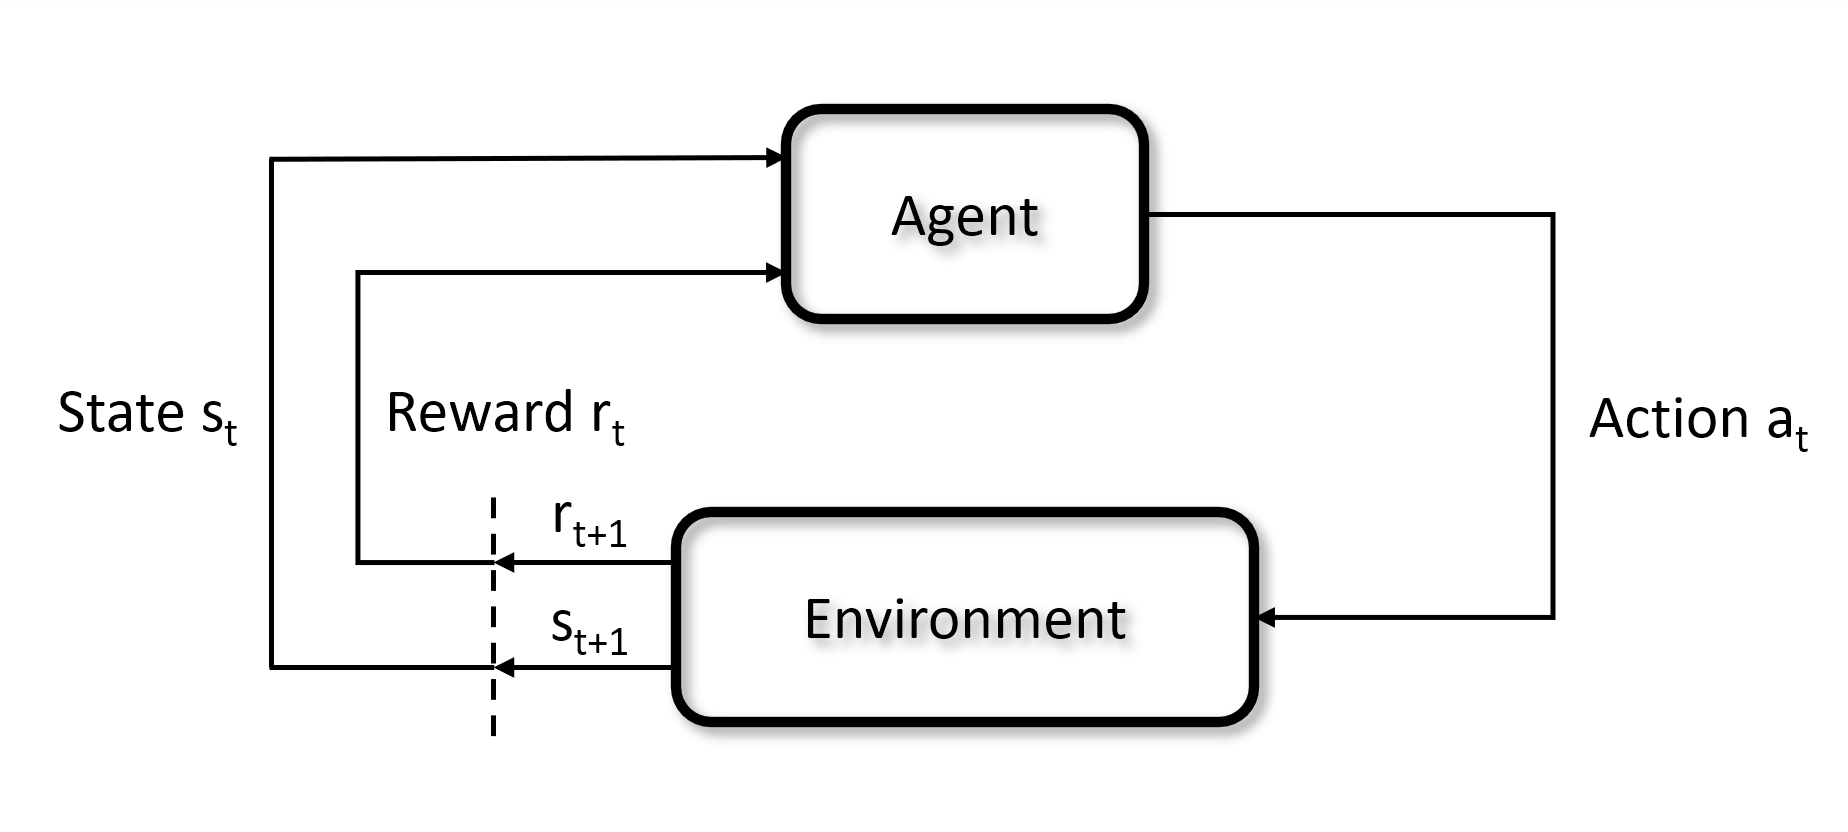
\includegraphics[width=14cm, keepaspectratio]{images/mdp/int_schema.png}
            \caption{A schema of the Agent-Environment Interaction.}
            \label{fig:mdp}
        \end{figure}
        
        \subsection{State, Action and Reward}
            \label{subs:sar}
            The interaction between the Agent and the Environment is articulated in a sequence of discrete time-steps. At each time-step \textit{t}, the Agent receives a representation of the Environment, called State ($s_t\in \mathbf{S}$). Then the Agent selects an Action ($a_t\in \mathbf{A}$)  to be executed in the Environment. As a consequence of the aforementioned Action $a_t$, at time-step \textit{t+1} the Agent receives a Reward ($r_{t+1}\in \mathbf{R}$) and perceives a new State $s_{t+1}$. The cyclic nature of this behavior can be observed in Figure \ref{fig:mdp}. 
            \\\\
            The interaction between the Agent and the Environment along the time-steps produces a trajectory: $s_0, a_0, r_1, s_1, a_1, r_2, s_2, ...$, which can be finite or infinite depending on the Time Horizon of the MDP.
            \\\\
            The set of all states $\mathbf{S}$ is called State Space, the set of all actions $\mathbf{A}$ is called Action Space. States and actions can be either Discrete or Continuous depending on the Environment properties. At last, $\mathbf{R}$ is the Reward Function, which returns a reward for each triple $(s, a, s')$ and thus can be defined as: $\mathbf{R}: \mathbf{S} \times \mathbf{A} \times \mathbf{S} \rightarrow \mathds{R} $. For the sake of completeness, collected rewards can be either negative or positive real values and depending on the sign they can be referred as costs. If the reward signal is formulated as a sequence of negative real values, the Reward function can also be called Cost Function.
            
        \subsection{Markov Property and State-Transition Probabilities}
            \label{subs:markov}
            A defining property of the Markov Decision Process is the Markov Property, which states: 
            
            \begin{definition}[Markov Property]
                \label{def:markov}
                A stochastic process $S_{t}$ is said to be Markovian if and only if:
                \[ P \left( S_{t+1} = s' | S_{t} = s, S_{t-1} = s_{t-1}, ..., S_{1} = s_1, S_{0} = s_0 \right) = P \left( S_{t+1} = s' | S_{t} = s \right)\]
                
                where the stochastic process $S_t$ is the trajectory the Agent follows in the environment. Therefore the State $s$ constitute a sufficient statistic for the future sequence of states.
            \end{definition}
            Intuitively, the Markov Property states that each state $s$ must include all necessary information and aspects of the interaction between the Agent and the Environment that occurred before the Agent reached the said state and previous history is not needed in order to plan future actions. \newline
            This property has fundamental consequences since it enables decision-making that relies only on the knowledge of the current state and reward and not on the full trajectory experienced by the Agent. Upon this property, the Dynamics of the MDP can be defined as: 
            
            \begin{definition}[Dynamics of the MDP]
                \label{def:dynamics}
                \[P : \mathbf{S} \times \mathbf{A} \times \mathbf{S} \times \mathbf{R} \rightarrow [0, 1] \]
                \[P(s', r | s, a) \doteq \mathbf{E} \left[S_{t+1}=s', R_{t+1}=r | S_t=s, A_t=a \right]\]
            \end{definition}
            
            Thus, the probability of the Agent reaching a new state $s_{t+1}$ receiving a reward $r_{t+1}$ only depends on the previous state $s_t$ and the following action $a_t$. The entire trajectory traversed by the Agent so far is not necessary. The dynamics of the MDP define the entire behaviour of the interaction.
            \\\\
            At last, derived from the Dynamics of the system, the State-Transition Probability Function defines the probability of reaching a certain new state $s_{t+1}$ knowing the current state $s_t$ and action $a_t$:
            
            \begin{definition}[State-Transition Probability Function]
                \label{def:transprob}
                \[p : \mathbf{S} \times \mathbf{A} \times \mathbf{S} \rightarrow [0, 1] \]
                \[ p(s' | s, a) \doteq \sum_{r\in \mathbf{R}} P(s', r | s, a) \]
            \end{definition}
            
            State transitions can be either Deterministic or Stochastic, depending on the values of the State-Transition Probability Function, and thus, ultimately, on the Dynamics of the system. Deterministic State-Transition Probability functions assigns to each triple $(s, a, s')$ either probability 0 or probability 1, denoting a rather simple Environment in which each action provides clear and repeatable results. Stochastic State-Transition Probability functions, instead, assigns continuous probability values to each triple $(s, a, s')$, denoting a more complex environment in which actions' consequences are variable in each state. \newline
            To shorten the notation, an Environment characterized by Deterministic State-Transition Probability function can be simply called Deterministic Environment and, analogously, Stochastic Environments can be defined. \newline
            Intuitively, learning in a Deterministic Environment is much simpler than in a Stochastic Environment, due to the fact that the decisions taken by the Agent will have fixed and repeatable consequences. In Stochastic Environment, instead, selecting the same action $a$ twice in the same state $s$ may lead to different next states $s'$ and, as a consequence, the Agent will need more experience in the Environment in order to correctly assess all possible outcomes.
            
        \subsection{Markov Decision Process}
            Now that all its components have been presented, a formalized definition of a Markov Decision Process can be given:
            
            \begin{definition}[Markov Decision Process (MDP)]
                \label{def:mdp}
                A Markov Decision Process (or MDP) is a 4-tuple:
                \[ \langle \mathbf{S}, \mathbf{A}, p, \mathbf{R} \rangle\]
                where:
                \begin{itemize}
                    \setlength\itemsep{0em}
                    \item $\mathbf{S}$ is the set of states, called State Space;
                    \item $\mathbf{A}$ is the set of actions, called Action Space;
                    \item $p$ is the State-Transition Probability function;
                    \item $\mathbf{R}$ is the Reward function.
                \end{itemize}
            \end{definition}
            
        \subsection{Policy, Value and Action-Value Functions}
            \label{subs:PVQ}
            
            \begin{figure}[t]
                \centering
                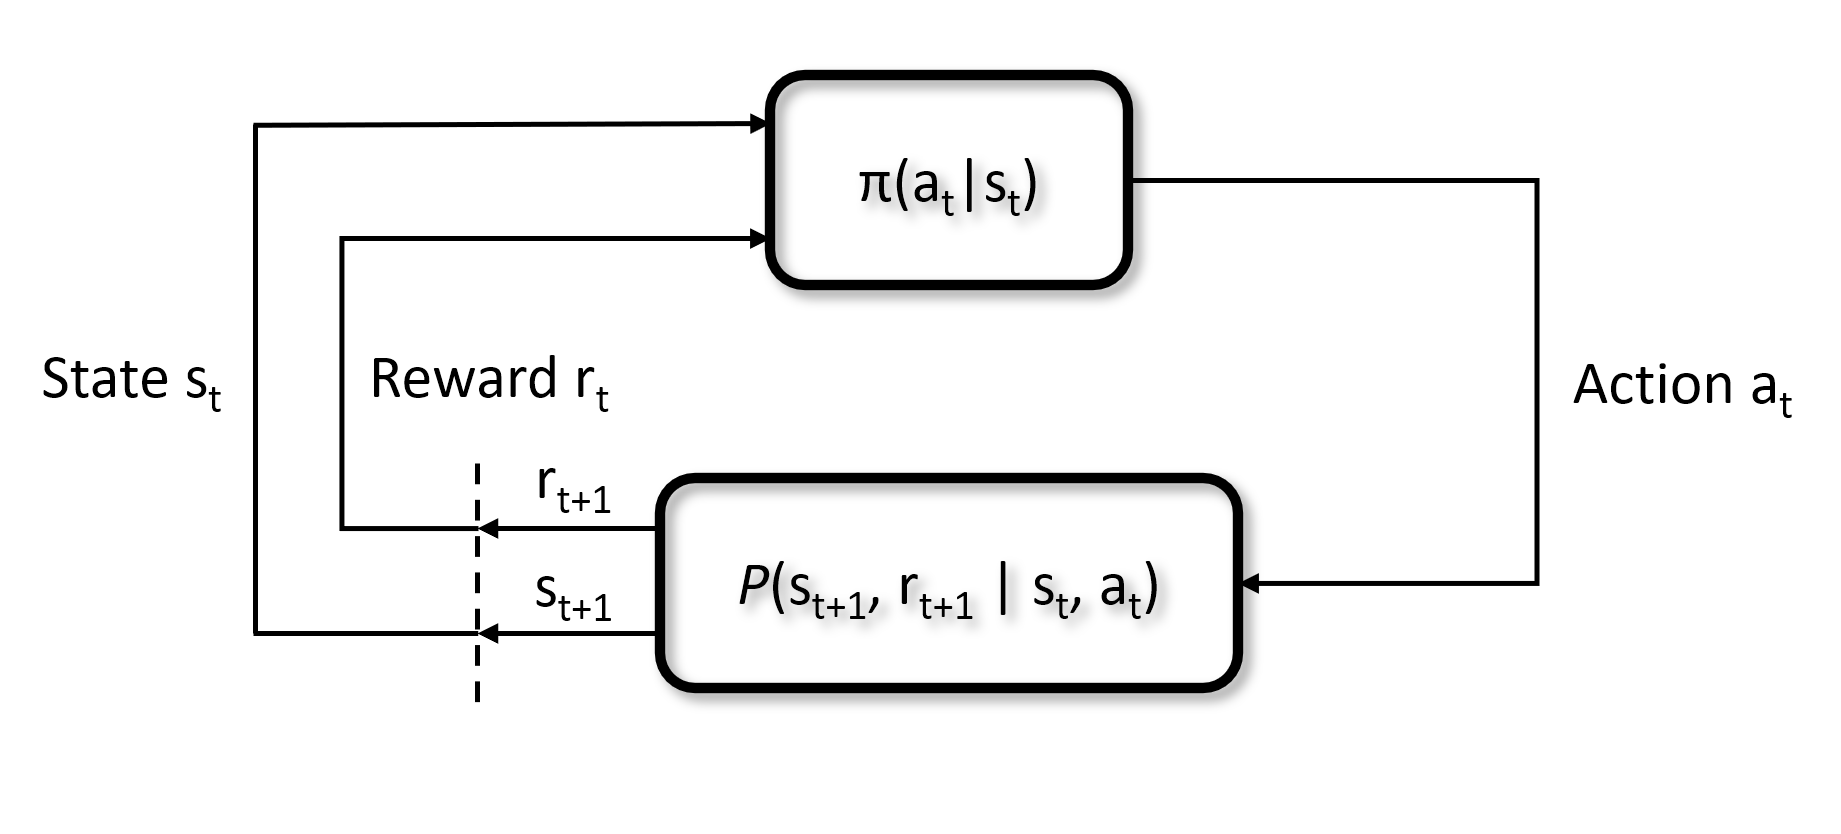
\includegraphics[width=14cm, keepaspectratio]{images/mdp/int_schema_def.png}
                \caption{A schema of the Agent-Environment Interaction denoting the purpose of the Policy Function $\pi$ and Dynamics of the System $P$.}
                \label{fig:int_schema_def}
            \end{figure}
            
            As described so far, the Environment evolution through time is guided by the Dynamics of the MDP, while the Agent is able to choose an action at each step of the trajectory, traversing different states in order to reach its goal, which is defined by the reward function. 
            
            \begin{definition}[Policy]
                \label{def:policy}
                A Policy is a function that returns the probability of selecting each available action $a$ when the Agent is in a state $s$. It is denoted as:
                \begin{align*}
                  \pi : \mathbf{S} \times \mathbf{A} &\rightarrow [0, 1]\\
                  (s,a) &\mapsto \pi(a|s).
                \end{align*}
            \end{definition}

            A Policy defines the behaviour of the Agent that follows it while interacting with the Environment. In figure \ref{fig:int_schema_def}, the interaction between the Agent and the Environment is updated, showing more precisely the role of the Policy function and the Dynamics of the System. Once the behaviour of the Agent has been defined through a Policy function, it is important to also be able to evaluate the goodness of the said behaviour. For this reason, it is important to define the following Discounted Return:
            
            \begin{definition}[Discounted Return]
                \label{def:return}
                The Discounted Return is the discounted sum of the rewards collected along the trajectory drawn by following a certain policy $\pi$:
                \[ \mathbf{R_{0}^{\pi}} \coloneqq \sum_{t=0}^{T} \gamma^{t} r_t,  \;\; 0 \leq \gamma \leq 1  \]
                where \textit{T} is the time horizon of the trajectory, $\gamma$ is the Discount Factor and $r_t$ is the reward collected by the Agent at time-step t.
            \end{definition}
            
            The purpose of the Agent is selecting the actions, hence the policy, that maximize the Discounted Return. As a consequence, the Agent needs to choose actions that enables future rewards as well as collecting good immediate rewards. The value of the Discount Factor $\gamma$ implicitly determines the importance within the Discounted Return of the future collected rewards.
            
            \begin{definition}[State-Value Function]
                \label{def:valuefun}
                The Value of a state $s$ following a policy $\pi$ is defined as the Expected Discounted Return of the Agent that starts at state $s$ and follows policy $\pi$ thereafter. 
                \[ v_{\pi}\left(s\right) \coloneqq \mathbf{E}_{\pi} \left[ \mathbf{R}_{t}^{\pi} | S_{t}=s\right] = \mathbf{E}_{\pi} \left[ \sum_{k=0}^T \gamma^k r_{t + k} | S_{t}=s\right] \]
                where the expectation is taken over all the possible trajectories that can be obtained by following $\pi$.
                Furthermore, the function $v_{\pi}$ is called State-Value function for policy $\pi$.
            \end{definition}
            
            By correctly estimating the Value of the states by experience, the Agent is able to determine the quality of being in each state, accordingly to the given policy. A further step can be taken in the direction of assessing the quality of a specific action chosen in a specific state:
            
            \begin{definition}[Action-Value Function]
                \label{def:actionvaluefun}
                The Value of choosing an action $a_t$ in a state $s_t$ following a policy $\pi$ is defined as the Expected Discounted Return of the Agent that starts at state $s_t$, selects the action $a_t$ and follows policy $\pi$ thereafter. 
                \[ q_{\pi}\left(s,a\right) \doteq \mathbf{E}_{\pi} \left[ \mathbf{R}_{t}^{\pi} | S_{t}=s, A_{t}=a\right] = \mathbf{E}_{\pi} \left[ \sum_{k=0}^T \gamma^k r_{t + k + 1} | S_{t}=s, A_{t}=a\right]\]
                where the expectation is taken over all the possible trajectories that can be drawn by following $\pi$.
                Furthermore, the function $q_{\pi}$ is called Action-Value function for policy $\pi$.
            \end{definition}
            
            Similarly to the Value Function, by correctly estimating the Action-Values the Agent can determine the quality of choosing an action in a state, accordingly to the given policy. 
            
        \subsection{Bellman Equations}
            \label{subs:bellman}
            From the definition of Discounted Return, a very important property arises:
            
            \begin{property}[Recursivity of the Discounted Return]
                \label{prop:recreturn}
                By unrolling the sum over the time-steps of the Discounted Return:
                \[ \mathbf{R}_{t}^{\pi} \doteq r_{t} + \gamma^{1} r_{t+1} + \gamma^{2} r_{t+2} + ... = r_{t} + \gamma \left( r_{t+1} + \gamma^{1} r_{t+2} + ... \right) = r_{t} + \gamma \mathbf{R}_{t+1}^{\pi}  \]
                This property is valid for each time-step $t \leq T$, where $\mathbf{R}_{T}^{\pi} = 0$.
            \end{property}
            
            This recursive relationship directly reflects on the properties of the Value Function, since its definition relies on the Discounted Return. From the definition of $v_{\pi}$:
            
            \begin{definition}[Bellman Equation for Value Functions]
                \label{def:bellmanvalue}
                \[ v_{\pi}(s) \doteq \mathbf{E}_{\pi} \left[ \mathbf{R}_{t}^{\pi} | S_{t} = s \right] =
                    \mathbf{E}_{\pi} \left[ r_{t} + \gamma \mathbf{R}_{t+1}^{\pi} | S_{t} = s \right] \]
                Then, by unrolling the expectation over all the possible trajectories drawn by following $\pi$:
                \begin{align*}
                    v_{\pi}(s) &= \sum_{a \in \mathbf{A}} \pi(a|s) 
                                \sum_{\substack{s' \in \mathbf{S}\\r \in \mathbf{R}}} P(s', r | s, a) 
                                \left[ r + \gamma \mathbf{E}_{\pi} \left[ \mathbf{R}_{t+1}^{\pi} | S_{t+1} = s' \right] \right] \\        
                                &= \sum_{a \in \mathbf{A}} \pi(a|s) 
                                \sum_{\substack{s' \in \mathbf{S}\\r \in \mathbf{R}}} P(s', r | s, a) 
                                \left[ r + \gamma v_{\pi}(s') \right]
                \end{align*}
                where $\pi(s|a)$ represents the probability of choosing action a being in state s when following policy $\pi$.
            \end{definition}
            
            The Bellman Equation directly relates the value of a certain state $s$ ($v_{\pi}(s)$) with the value of all its successor states $s'$ ($v_{\pi}(s')$). Starting from s, each possible triple $(a, r, s')$ is evaluated: the sum of the immediate reward $r$ collected by choosing action $a$ and the expected discounted future reward represented by $\gamma v_{\pi}(s')$ is weighted by its probability $\pi(a|s)P(s',r|s,a)$; and the results are summed together. The Value function $v_{\pi}$ is the only solution to the Bellman Equation and this property strongly reflects on the practical point of view. Infact, the Bellman Equation constitutes a basis for many ways of correctly estimating $v_{\pi}$, thus enabling policy comparison and improvement. \newline
            Similarly, the Bellman Equation for the Action-Value Function $q_{\pi}$ can be defined:
            \begin{definition}[Bellman Equation for Action-Value Functions]
                \label{def:bellmanaction}
                \[ q_{\pi}(s, a) \doteq \mathbf{E}_{\pi} \left[ \mathbf{R}_{t}^{\pi} | S_{t} = s, A_{t} = a\right] =
                    \mathbf{E}_{\pi} \left[ r + \gamma \mathbf{R}_{t+1}^{\pi} | S_{t} = s, A_{t} = a \right] \]
                Then, by unrolling the expectation over all the possible trajectories drawn by following $\pi$:
                \begin{align*}
                    q_{\pi}(s,a) &= \sum_{\substack{s' \in \mathbf{S}\\r \in \mathbf{R}}} P(s', r | s, a)
                                \left[ r + \gamma \mathbf{E}_{\pi} \left[ \mathbf{R}_{t+1}^{\pi} | S_{t+1} = s'\right] \right] \\        
                                 &= \sum_{\substack{s' \in \mathbf{S}\\r \in \mathbf{R}}} P(s', r | s, a)
                                \left[ r + \gamma v_{\pi}(s') \right]
                \end{align*} 
            \end{definition}
            The main difference is the lack of a summation over all the actions, since the action is fixed by the action-value function itself. Furthermore, the link between Value and Action-Value functions is now apparent:
            
            \begin{property}[Relationship between $v_{\pi}$ and $q_{\pi}$]
                \label{prop:linkvq}
                \[ v_{\pi}(s) = \sum_{a \in \mathbf{A}} \pi(s|a) q_{\pi}(s,a)\]
                Intuitively, the Value Function of a state $s$ is the weighted sum of the values of the actions $a$ available in $s$, whereas the weights are the probability assigned by policy $\pi$ to each action $a$.
            \end{property}
            
            
        \subsection{Optimal Policy, Value and Action-Value Functions}
            \label{subs:opt}
            Finally, the Optimal Policy w.r.t. the Environment's Dynamics can be defined. Each possible policy in the environment, along with the reward function, determines the values of each state of the said environment. Hence, the set of policies can be partially ordered by using the values they induce in each state.
            
            \begin{definition}[Optimal Policy]
                \label{def:opt}
                A policy $\pi^*$ is said to be optimal if and only if:
                \[ v_{\pi^*}(s) \geq v_{\pi}(s),\;\;\forall s: s \in \mathbf{S} \land \forall \pi\]
            \end{definition}
            
            The Optimal Policy $\pi^{*}$ may not be unique, but they all share the same Value Function, which is the Optimal Value Function:
            
            \begin{definition}[Optimal Value Function]
                \label{def:optvalue}
                Denoted as $v_{*}$, the Optimal Value Function is the value function related to the optimal policy and hence:
                \[ v_{*}(s) \doteq \max_{\pi} v_{\pi}(s),\;\;\forall s \in \mathbf{S}\]
            \end{definition}
            
            Similarly, the Optimal Action-Value Function is shared among all the optimal policy $\pi^{*}$ and it can be defined:
            
            \begin{definition}[Optimal Action-Value Function]
                \label{def:optactionvalue}
                Denoted as $q_{*}$, the Optimal Action-Value Function is the action-value function related to the optimal policy and hence:
                \[ q_{*}(s, a) \doteq \max_{\pi} q_{\pi}(s, a),\;\;\forall s \in \mathbf{S} \land \forall a \in \mathbf{A}\]
            \end{definition}
            
        \subsection{Bellman Optimality Equations}
            \label{subs:optbellman}
            Since $v_{*}(s)$ and $q_{*}(s,a)$ are respectively Value and Action-Value functions for a policy, they must satisfy the recursive requirements stated by the Bellman Equations.
            
            \begin{definition}[Bellman Optimality Equation for $v_{*}$]
                \label{def:bellmanoptvalue}
                \begin{align*}
                    v_{*}(s)    &= \max_{\pi} \sum_{a \in \mathbf{A}} \pi(a|s) 
                                \sum_{\substack{s' \in \mathbf{S}\\r \in \mathbf{R}}} P(s', r | s, a) 
                                \left[ r + \gamma v_{\pi}(s') \right] \\        
                                &= \max_{a} 
                                \sum_{\substack{s' \in \mathbf{S}\\r \in \mathbf{R}}} P(s', r | s, a) 
                                \left[ r
                                + \gamma v_{*}(s') \right]
                \end{align*}  
                where max operator over $\pi$ and the summation of $\pi(a|s)$ over all the actions have been condensed in the maximum over all the available actions.
            \end{definition}
            
            Intuitively, the Bellman Optimality Equation for $v_{*}$ states that $v_{*}$ represents the expected discounted return the agent can collect by choosing the best action available in each state. As usual, a similar equation is valid for $q_{*}(s,a)$:
            
            \begin{definition}[Bellman Optimality Equation for $q_{*}$]
                \label{def:bellmanoptaction}
                \begin{align*}
                    q_{*}(s,a)  &= \max_{\pi}
                                \sum_{\substack{s' \in \mathbf{S}\\r \in \mathbf{R}}} P(s', r | s, a) 
                                \left[ r + \gamma v_{\pi}(s') \right] \\        
                                &= \max_{\pi}
                                \sum_{\substack{s' \in \mathbf{S}\\r \in \mathbf{R}}} P(s', r | s, a) 
                                \left[ r + \gamma \sum_{a' \in \mathbf{A}} \pi(s'|a') q_{\pi}(s',a') \right]\\
                                &= \sum_{\substack{s' \in \mathbf{S}\\r \in \mathbf{R}}} P(s', r | s, a) 
                                \left[ r + \gamma \max_{a' \in \mathbf{A}} q_{*}(s', a') \right]
                \end{align*}
                where max operator over $\pi$ and the summation of $\pi(a|s)$ over all the actions have been condensed in the maximum over all the available future actions.
            \end{definition}
            
            At last, all the notions presented can be linked together. The optimal value function $v_{*}$ assigns to a state the expected return the agent is able to achieve by following the optimal policy $\pi_{*}$. Therefore, the Agent can behave greedily within respect to the optimal value function and expect to achieve the optimal policy: even if each action $a$ is chosen by evaluating immediate consequences in terms of the value function $v_{*}$, the definition of value function itself ensures that it is optimal in the long-term. Similar considerations can be made about the optimal action-value $q_{*}$, which also contains direct information regarding which action must be selected by the Agent, without explicitly knowing the next states. 
         

        % \subsection{Same objective, different technologies}
        %     During the history of research in the Reinforcement Learning field, numerous and various algorithms have been studied along with several demonstrations of convergence to the Optimal Value functions in order to ensure the possibility of reaching good performances in the Environment. In 1957, \pcite{dynamicprogramming} establishes the bases for \pcite{policyiteration}, in which Policy Iteration is presented. During the following decades, other famous and instructive algorithms such as Value Iteration (\pcite{valueiteration}), based on Policy Iteration; Q-Learning (\pcite{qlearning}) and SARSA (\pcite{sarsa}) have been constructed, along with numerous variations not mentioned for the sake of brevity, which are part of the Temporal-Difference Learning paradigm (\pcite{temporaldifference}). From those years to the beginning of this century, \pcite{REINFORCE}, \pcite{policygradient} and \pcite{kakade2002} pose the basis for a new paradigm: Policy-Gradient Methods and later on Natural-Gradient methods. Eventually, the explosion of Deep Learning in the last decade contaminated the field of Reinforcement Learning, leading to the revision of known methods and the construction of completely new algorithms. In 2014, Deep Q-Network was presented as a Deep Learning variant of Q-Learning (\pcite{dqn}) and short after Deep Deterministic Policy Gradient followed (\pcite{ddpg}) as a continuous control variant. At last, new algorithms such as Trust Region Policy Optimization (\pcite{trpo}, presented in Section \ref{sota:trpo}) and Proximal Policy Optimization have been presented in very recent years. 
        %     \\\\
        %     Regardless of the historical period, each one of the cited algorithms and many others relies on the Markov Decision Process framework and, as a consequence, they share a common objective: correctly and efficiently estimating the Expected Return, either in form of Value function or Action-Value function. Being able to quickly and precisely assess the quality of a Policy is a key aspect in order to tackle difficult task in complex environment within reasonable computational times. Thus, this is the main focus of the overall research.
    
    \newpage
    \section{Concepts on Delays in Reinforcement Learning}
    \label{defproblem:delays}
        The fundamental aspects and importance of the Markov Decision Process framework have been presented so far, highlighting the major definitions and concepts that enables further researches and studies in the Reinforcement Learning field. The simplicity of its concepts and structures allows for orderly defining complex Environments and structured Agents' behaviour. As the history of research testifies, Markov Decision Process has been proven to be a very useful and strong tool to rely on. \newline
        However, its simplicity also comes with a number of simplifications that do not hold in reality. Intuitively, whenever the model constructed by using the MDP framework is not fully aligned with reality, the Agent perceptions and decisions can not be fully precised and tailored for the actual environment. The effects of a mismatch between Agent perceptions and reality may affect the real-world performance of the Agent by a certain amount, that is proportional to how relevant the mismatch is within respect to the task of the Agent. \newline
        There is a number of precautions that can be taken to minimize the risk, relying on the broad definitions of State, Action and Reward that the MDP framework provides. Modeling states in such a way to hold correct and precise information and providing them in an appropriate format; defining Agent actions that are tailored for a precise interaction with the Environment and so on. However, there exists a number of concepts in reality that are simply not natively supported by the MDP framework. One such concept is the concept of Delay.
        
        \subsection{Observation, Action and Reward Delays}
            Within the MDP framework, there is a number of implicit assumptions that are in contrast with what really happens in reality. As \pcite{delay:dmdp} points out in its introduction, a group of three particular strong assumptions can be highlighted:
            \begin{itemize}[topsep=0.5em, partopsep=0.5em]
                \setlength\itemsep{0em}
                \item States are always immediately available to the Agent;
                \item Actions have immediate consequences on the Environment;
                \item Rewards are collected instantly after the action has been chosen.
            \end{itemize}
            These behaviours are seldom found in real-world application, where a number of complications exists, even only due to the Agent implementation. States are not always immediately available: the environment may not provide all the current information needed at all times, the Agent may need time in order to process state information or to transmit it to all its component (i.e. Multi-Agent Systems in which data needs to be transmitted and processed by different single-agents). Actions take a specific amount of time in order to be actuated in the Environment or they may need time in order to actually produce effects in the environment. Rewards may not be measurable instantaneously, in the sense that benefits or cost produced by the Agent's decision may not be accessible immediately, but rather need some time in order to be assessed, such in the case of medical assistance.
            \\\\
            From these intuitive presentation of the three assumptions, more precise definitions can be formulated:
            
            \begin{definition}[Observation Delay]
                \label{def:obsdelay}
                It is called \textit{Observation Delay}, $d_o$, the delay, represented in number of time-steps, between the time-step $t$ in which the Agent reaches a state $s$ and the time-step $t+d_o$ in which the Agent collects the information about this state.
            \end{definition}
            
            Figure \ref{fig:o_delay} shows how the Agent is affected by the presence of the Observation Delay $d_o$. The Agent perception of the current state is delayed by $d_o$ step: the selected action $a_t$ is executed on a currently unobserved state $s_{t}$ while observing a past state $s_{t-d_{o}}$ and the reward signal $r_t$ is associated to the transition $(s_{t-d_{o}-1}, a_{t-d_{o}-1}, s_{t-d_{o}})$ instead of the transition $(s_{t-1}, a_{t-1}, s_{t})$. This entails that the Agent's decisions are not based on up-to-date knowledge about the environment, which may prevent the Agent from reacting in time to certain events.
            
            \begin{definition}[Execution Delay]
                \label{def:execdelay}
                It is called \textit{Execution Delay}, $d_a$, the delay, represented in number of time-steps, between the time-step $t$ in which the Agent chooses action $a$ and the time-step $t+d_a$ in which the action $a$'s effects take place in the environment.
            \end{definition}
            
            Figure \ref{fig:a_delay} shows the effect of the Execution Delay $d_a$ on the Agent's perceptions. The chosen action $a_t$ will affect the future transition $(s_{t+d_{a}}, a_t, s_{t+d_{a}+1})$, while the next transition is the effect of the action $a_{t-d_{a}}$, chosen $d_a$ time-step before. This effectively disrupts the ability of the Agent of assessing correctly the nature of causality that exists in the environment. 
            
            \begin{definition}[Reward Delay]
                \label{def:rewdelay}
                It is called \textit{Reward Delay}, $d_r$, the delay, represented in number of time-steps, between the time-step $t$ in which the Agent chooses action $a$ and the time-step $t+d_r$ in which the Agent receives the reward $r$ as a consequence of $a$.
            \end{definition}
            
            Figure \ref{fig:r_delay} explains reward collection under the presence of a Reward Delay $d_r$. Reward collected as a result of the transition $(s_t, a_t, s_{t+1})$ is available $d_r$ time-step in the future $(r_{t+d_{r}})$, while the actually collected reward $r_{t+1}$ is the result of a past transition. This causes a misalignment between the decisions and the reward collected, which prevents correct assessment of the actions' quality.
            
            \begin{figure}
                \centering
                
                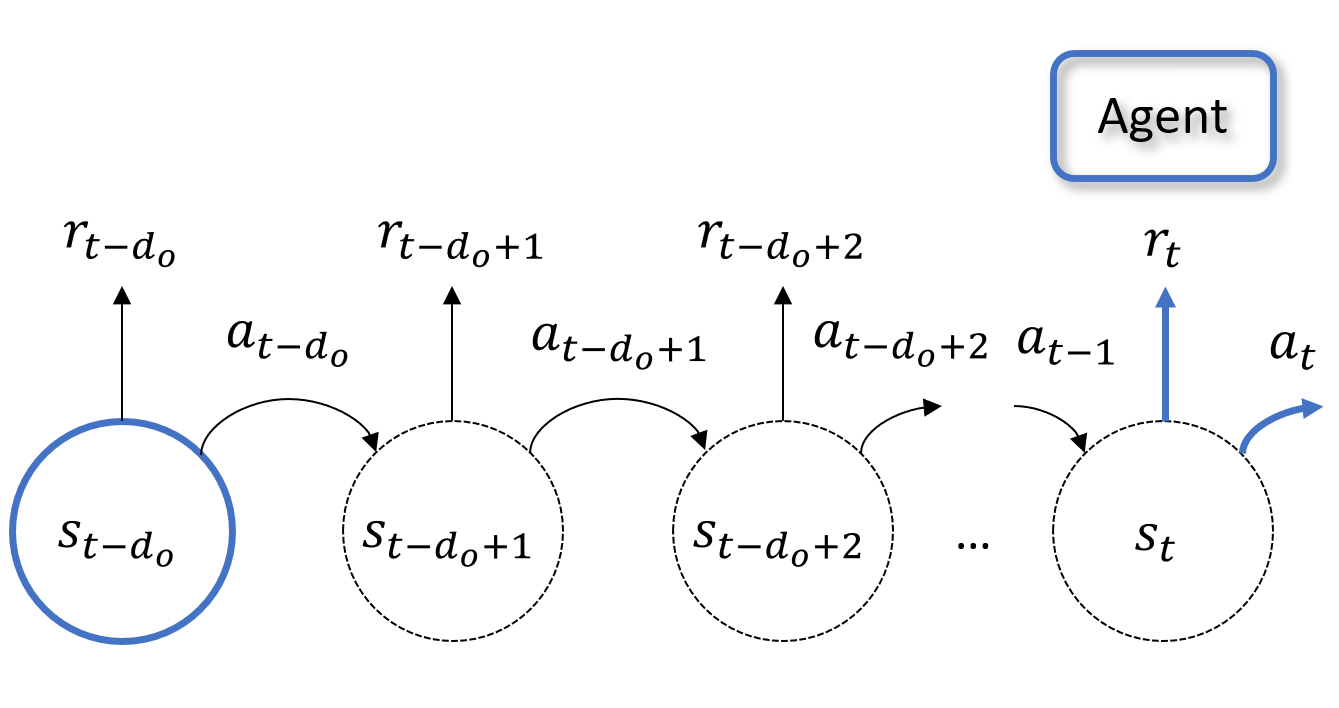
\includegraphics[width=11cm, keepaspectratio]{images/dmdp/o_delay.png}
                \caption{Observation Delay ($d_o$) effects. Agent's position is represented by the state aligned with it, while its perception is highlighted in light blue. The observed current state is $s_{t-d_{o}}$, but the actual current state is $s_{t}$.}
                \label{fig:o_delay}
                
                \vspace{0.5cm}
                
                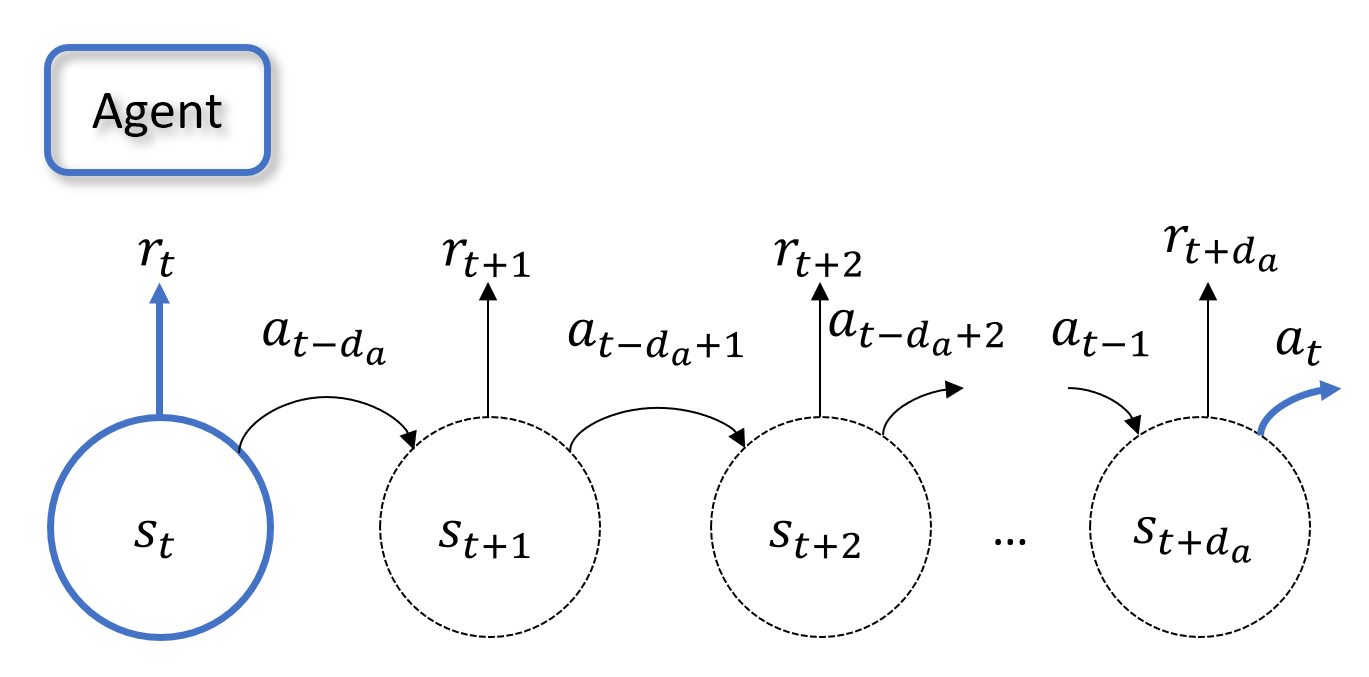
\includegraphics[width=11cm, keepaspectratio]{images/dmdp/a_delay.png}
                \caption{Execution Delay ($d_a$) effects. Agent's position is represented by the state aligned with it, while its perception is highlighted in light blue. The currently chosen action $a_t$ will actually take effect in $d_a$ steps, while the actual cause of the next transition is action $a_{t-d_{a}}$.}
                \label{fig:a_delay}
                
                \vspace{0.5cm}
                
                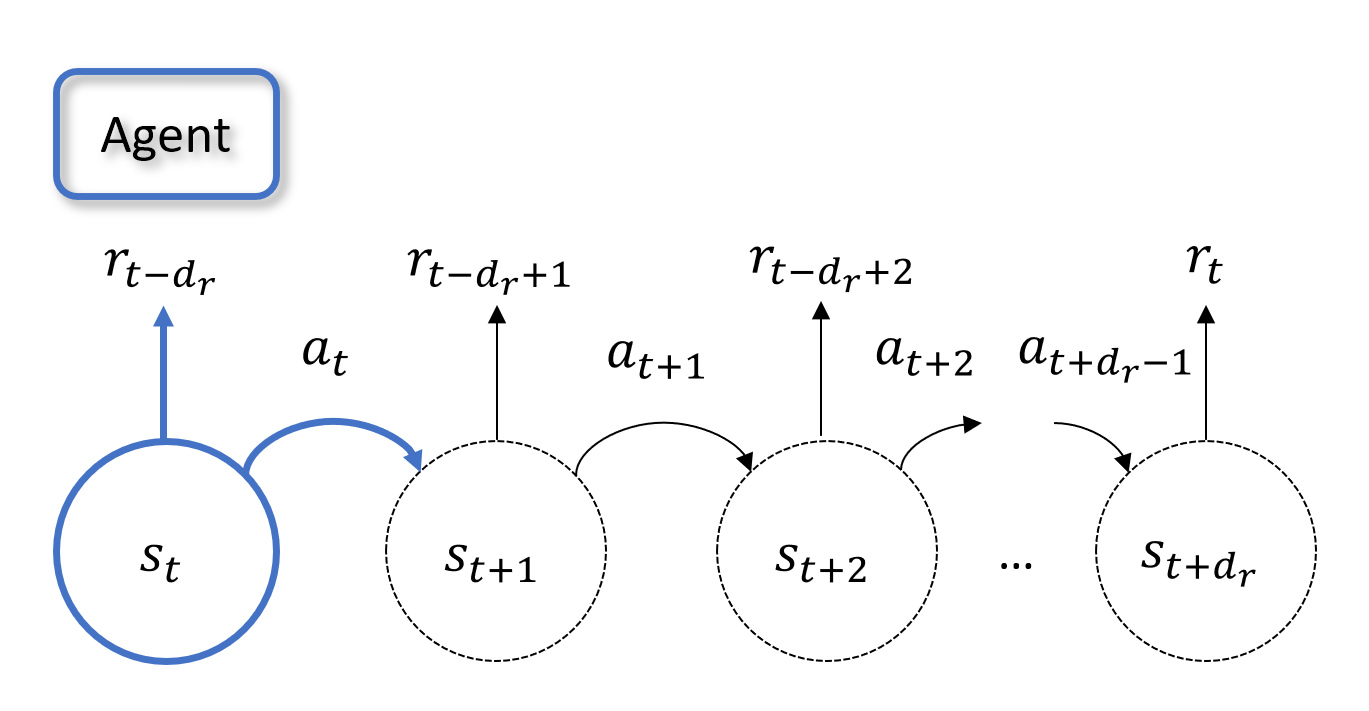
\includegraphics[width=11cm, keepaspectratio]{images/dmdp/r_delay.png}
                \caption{Reward Delay ($d_r$) effects. Agent's position is represented by the state aligned with it, while its perception is highlighted in light blue. The reward signal is collected $d_r$ time-step later w.r.t. the actual transition that generated it.}
                \label{fig:r_delay}
                
            \end{figure}
            
        \subsection{Delayed Markov Decision Process}
            Starting for the definitions of delays given the previous section, the MDP framework can be expanded in a straightforward manner, by including the delays:
            
            \begin{definition}[Observation Delayed MDP]
                \label{def:odmdp}
                An Observation Delayed MDP (or OD-MDP) is a 5-tuple:
                \[ \langle \mathbf{S}, \mathbf{A}, p, \mathbf{R}, d_o \rangle\]
                where $\mathbf{S}$ is the State Space, $\mathbf{A}$ is the Action Space, $p$ is the State-Transition Probability function, $\mathbf{R}$ is the Reward function and $d_o$ is the Observation Delay.
            \end{definition}
            
            In this definition, the term \textit{observation} is used as an alternative of the term state, although it may be more general in the sense that it also includes cases in which the state is not fully available to the Agent (i.e. Partially-Observed MDP).
            
            \begin{definition}[Execution Delayed MDP]
                \label{def:edmdp}
                An Execution Delayed MDP (or ED-MDP) is a 5-tuple:
                \[ \langle \mathbf{S}, \mathbf{A}, p, \mathbf{R}, d_a \rangle\]
                where $\mathbf{S}$ is the State Space, $\mathbf{A}$ is the Action Space, $p$ is the State-Transition Probability function, $\mathbf{R}$ is the Reward function and $d_a$ is the Execution Delay.
            \end{definition}
            
            \begin{definition}[Reward Delayed MDP]
                \label{def:rdmdp}
                A Reward Delayed MDP (or RD-MDP) is a 5-tuple:
                \[ \langle \mathbf{S}, \mathbf{A}, p, \mathbf{R}, d_r \rangle\]
                where $\mathbf{S}$ is the State Space, $\mathbf{A}$ is the Action Space, $p$ is the State-Transition Probability function, $\mathbf{R}$ is the Reward function and $d_a$ is the Reward Delay.
            \end{definition}
        
            Finally, the last three definitions can be combined in order to obtain a general definition that takes into account for every type of delay:
            
            \begin{definition}[Delayed MDP]
                \label{def:dmdp}
                A Delayed MDP (or DMDP) is a 7-tuple:
                \[ \langle \mathbf{S}, \mathbf{A}, p, \mathbf{R}, d_o, d_a, d_r \rangle\]
                where $\mathbf{S}$ is the State Space, $\mathbf{A}$ is the Action Space, $p$ is the State-Transition Probability function, $\mathbf{R}$ is the Reward function, $d_o$ is the Observation Delay, $d_a$ is the Execution Delay, $d_r$ is the Reward Delay.
            \end{definition}
            
            In general, the presence of delays can be represented by a mixture of the examples provided in Figures \ref{fig:o_delay}, \ref{fig:a_delay} and \ref{fig:r_delay}, showing a much more complex interaction between the Agent and the Environment than the MDP framework interaction. \newline
            The definition of Delayed MDP is the starting point in defining how the presence of delays can be modeled in order to fit within the already widely used MDP framework. However, it also brings with itself some significant simplification which will be addressed in the following sections.
            
            \subsubsection{Time-Discretization Assumption}
                As \pcite{delay:memoryless} observe, there is no guarantee that the amount of time delay is an integer multiple of the sampling time that regulates the time dicretization for the Agent. As such, delayed information and actuation may not be aligned with the ticks of time that the Agent is following. Infact, delays definitions (Definition \ref{def:obsdelay}, \ref{def:execdelay} and \ref{def:rewdelay}) measure the amount of delay in terms of an integer number of time-steps and they implicitly assume their alignment with the Agent discrete time. This assumption holds throughout this research and it allows for a stronger focus on other complications.
        
        \subsection{DMDP and Partially Observable MDP}
            \subsubsection{Markov Property in DMDP}
                \label{subs:markovmdp}
                As presented in Section \ref{subs:markov}, Markov Property (Definition \ref{def:markov}) represents the foundation upon which the entire MDP framework is based, along with all the collateral definitions. However, 
                Definitions \ref{def:odmdp} (OD-MDP) and \ref{def:edmdp} (ED-MDP) undermine the Markov Property implicitly. Infact, both OD-MDP and ED-MDP assume that the decision process taken by the Agent throughout its trajectories is based on a partial amount of information. \newline
                In an OD-MDP, the Agent is observing as current state $s_{t-d_{o}}$ which has been traversed a certain amount of time-step $d_o$ before and basing its decision-making process on it. This results in a violation of the Markov Property, because the past state $s_{t-d_{o}}$ does not constitute all necessary information regarding the previous interaction of the Agent with the Environment, but lacks of all the states traversed in the time-steps $t \in (t-d_{o}, t]$. Similarly, in an ED-MDP, the decision-maker is selecting actions which impact will take effect in a certain number of time-steps $d_a$ on an observed state $s_{t+d_{a}}$. Thus, the current state $s_t$ is not a sufficient to contain all necessary information in order to plan an action in $d_{a}$ time-steps, resulting again in a violation of the Markov Property. \newline
                Markov Property ensures that the Agent can plan its decisions using a sufficient amount of information, allowing a complete focus on the ability of the Agent of efficiently learning a well-performant policy. Introducing delays in the MDP formulation disrupts this assumption, introducing a new source of uncertainty and lack of knowledge, which in turn directly affects the performance of the Agent. This brings DMDPs close to Partially Observable MDP, which are also based on a decision-making process carried out upon incomplete information about the current state of the Agent.
        
            \subsubsection{Partially Observable MDP}
                \label{subs:pomdp}
                Partially Observable MDPs (POMDPs) are a special class of MDPs in which the Agent does not perceive the complete state $s_t$, but rather an observation $o_t$ resulting from it. The said observation $o_t$ is related to the actual state $s_t$ by an \textit{Observation Function}:
                
                \begin{definition}[Observation Function]
                    \label{def:pomdp-obsf}
                    An Observation Function is a function that assigns the probability of being in a certain state $s_t$ knowing a certain observation $o_t$. It is denoted as:
                    \[ O : \mathbf{S} \times \mathbf{O} \rightarrow [0, 1] \]
                    \[ O(s_t | o_t) \]
                    where $\mathbf{S}$ is the State Space and $\mathbf{O}$ is the Observation Space (i.e. the Set of all the possible Observations $o$). 
                \end{definition}
                
                This entails that the decision process carried out by an Agent in a POMDP is not based on the certainty of observing a state, but rather on the probability of being in a certain state, given the observation perceived. This concept is formalized in the definition of Belief State:
                
                \begin{definition}[Belief State]
                    \label{def:pomdp-belief}
                    A Belief State $\mathbf{B}$ is a probability distribution over all the possible states in the State Space $\mathbf{S}$, given the history of the observations $o_t$.
                \end{definition}
                
                The presentation of this concepts is actually interesting since they constitute a relationship with the DMDP class. In both frameworks, the Agent is planning its decisions using incomplete knowledge of the Environment and, for example, the concept of Belief State could be applicable to the current unobserved state $s_t$ in OD-DMDP or to the future state $s_{t+d_{a}}$ in ED-MDP. \newline
                Thus, several topics of research in the field of POMDP represents an interesting inspiration in order to formulate new solutions for the presence of delay in DMDP. Infact, some of this topics have been used as starting point for several concepts in future sections of this research and a more in-depth analysis is presented in Section \ref{sota:pomdp}.
            
        \subsection{Deterministic and Stochastic Delays}
        \label{sub:dmdp_stochdelays}
            The definition of DMDP provided in Definition \ref{def:dmdp} explicitly assumes that the different kinds of delay can be formulated as a constant integer number that counts the number of time-steps of delay experienced by the Agent. This assumption represents another simplification of the nature of real environments. Infact, there exists no guarantee that the amount of delay, for each of the three presented kinds, will remain constant throughout all the trajectories the Agent can experience. \newline
            A number of events can occur that has an impact on the amount of delays perceived by the Agent, which may be due to the complex environment properties that involves different mechanisms' interaction. For example, the effectiveness of a medical procedure can be assessed by observing the patient conditions, which in turn are governed by complex biological and chemical processes that require an almost per use-case basis amount of time. Data transmission's delays are governed by the rules of queues and traffics on the networks, which are seldom constant throughout time. Thus, it is important to take notice that delays are not constant and a proper, more complex, formulation may be necessary depending on the Environment. 
            \\\\
            For this purpose, Definition \ref{def:dmdp} of a DMDP can be divided in two more specific definitions:
            
            \begin{definition}[Constant Delayed MDP]
                \label{def:cdmdp}
                A Constant Delayed MDP (or CDMDP) is a 7-tuple:
                \[ \langle \mathbf{S}, \mathbf{A}, p, \mathbf{R}, d_o, d_a, d_r \rangle\]
                where $\mathbf{S}$ is the State Space, $\mathbf{A}$ is the Action Space, $p$ is the State-Transition Probability function, $\mathbf{R}$ is the Reward function, $d_o$ is the Observation Delay, $d_a$ is the Execution Delay, $d_r$ is the Reward Delay. Furthermore, $d_o$, $d_a$ and $d_r$ are constant integer values.
            \end{definition}
            
            \begin{definition}{Stochastic Delayed MDP: }
                \label{def:sdmdp}
                A Stochastic Delayed MDP (or SDMDP) is a 7-tuple:
                \[ \langle \mathbf{S}, \mathbf{A}, p, \mathbf{R}, d_o(t), d_a(t), d_r(t) \rangle\]
                where $\mathbf{S}$ is the State Space, $\mathbf{A}$ is the Action Space, $p$ is the State-Transition Probability function, $\mathbf{R}$ is the Reward function, $d_o(t)$ is the Observation Delay, $d_a(t)$ is the Execution Delay, $d_r(t)$ is the Reward Delay. Furthermore, $d_o(t)$, $d_a(t)$ and $d_r(t)$ represents discrete-time stochastic processes.
            \end{definition}
            
            
            \subsubsection{Impact of Delay's Stochasticity}
            Introducing stochastic delays in the MDP framework can have several tricky consequences to be handled. For each kind of delay, sequentiality is not guaranteed anymore. Observations may be perceived in a different order based on the sampled delay at each time-step: supposing $d_o(0) = 3$ and $d_o(1) = 1$, state $s_0$ will be observed at time-step $t=3$, while state $s_1$ will be observed at time-step $t=2$. The same issue is present with Execution Delay $d_a(t)$, which affects the order on which actions take effect on the environment, and Reward Delay $d_r(t)$, which affects the order of reward collection. It may happen that the Agent observes different states at the same time-step, different actions take effect in the same time-step or different rewards are collected together. Furthermore, it may also happen to collect a reward from an unobserved state, implicitly revealing information about it. \\\\
            Careful assumptions can be made in order to circumvent some of this problematic and difficult behaviours. For example, \pcite{delay:dmdp} assumes that, at each time-step, the Agent can either receive a new observation or experience one more step of delay and that the probability of collecting a reward from an unobserved state is zero. In turn, this assumption entails that the delay experienced by the Agent can only grow indefinitely with time, leading to an undesired scenario in which the Agent needs to wait for it to be reduced. Other works such as \pcite{delay:mbs} and \pcite{delay:memoryless} assume constant delays, respectively explicitly and implicitly, as a reasonable middle-ground and, at last, another viable option is formulating the stochastic delays as a well-known stochastic process, such as Poisson distribution (\pcite{delay:mmqm}). \newline
            Throughout this research, both Deterministic and Stochastic Delays are studied and tested and, similarly, a number of assumptions and a formulation are used for Stochastic Delays.
        
        \subsection{Known and Anonymous Delays}
            In Reinforcement Learning, there is no guaranteed that the Environment properties are fully disclosed to the Agent or to the researcher that is implementing the Agent. This is valid for the dynamics of the system as much as for the delays of the system. Infact, information about the amount of constant delay or about the stochastic process that produces the delay may not be available at all. In this case, the type of delay is said to be Anonymous and further steps must be taken in order to allow the Agent to learn the nature of the delay itself. Otherwise, if information about delays in the actual Environment is completely given or decided a priori for an Environment simulation, the delay is said to be Known. \newline
            For the purpose of this research, delays are known and simulated in the tested environments. This allows for a more focused study of the capability of the proposed method to act in presence of delay rather than of correctly assessing the amount and type of delay.
        
     \chapter{State of the Art}
    \label{chp:sota}
    In this Chapter, relevant State-of-the-Art algorithms, definitions and frameworks are presented. This Chapter is divided in two main sections. At first, Section \ref{sota:delay_approaches} is concerned with discussing the current existing approaches developed to tackle the problem of delays within the Reinforcement Learning framework and the most efficient algorithms that are used and have been proposed to cope with them. Afterwards, Section \ref{sota:pomdp} is dedicated to a branch of the Partially Observable MDP research and algorithms that have been instrumental for the formulation of the original proposed implementation.
    
    \section{State of the Art Approaches for Delays in RL}
        \label{sota:delay_approaches}
        In this section, three different approaches to the problem of delays are presented and their advantages and disadvantages are explained along with examples of new algorithms that have been developed using them as reference. Infact, they do not only constitute a practical mean of developing new and more efficient methods to cope with delays, but they are also instructive on a more broaded and conceptual way of tackling the problem of delays, which is why they are referred to as "approaches" and not as "algorithms". \newline
        In particular, Section \ref{subs:augmentedapproach} presents the Augmented-State approach, focused on including all available knowledge at each time-step in a new definition of state, denoted as extended state, which brings to the definition of a new MDP on top of the delayed one. Section \ref{subs:memorylessapproach} is instead dedicated to the Memoryless approach, based on developing Agents that learn only upon the last observed state, possibly modifying existing algorithm to align the sequence of delayed rewards; while Section \ref{subs:modelbasedapproach} is concerned with the Model-Based approach, which divides the action selection process into two steps, the first concerned on elaborating a representation of the current, unknown position of the Agent, the second provides action selection based on the aforementioned representation.
        
        \subsection{Augmented State Approach}
            \label{subs:augmentedapproach}
            The Augumented approach is the result of a combined effort to reduce the DMDP framework (Definition \ref{def:dmdp}) to the standard undelayed MDP framework (Definition \ref{def:mdp}) with a systematic process, which, in turn, would allow for the native application of existing state-of-the-art algorithms in delayed contexts.
            
            \subsubsection{State Augmentation for Execution Delay}
                At first, \pcite{delay:execaugment} shows that it is possible to refomulate a Constantly Delayed MDP with execution and reward delay as an undelayed MDP. This objective can be achieved by defining all the components of a new Markov Decision Process starting from the given delayed process.
                
                \begin{definition}[Augmented State Space $\mathbf{I_{a}}$]
                    \label{def:execaugmentstate}
                    Given a Constantly Delayed MDP with execution and reward delay $\langle \mathbf{S}, \mathbf{A}, p, \mathbf{R}, 0, d_a, d_r \rangle$,
                    a new \textit{augmented} state space $\mathbf{I_{a}}$ can be defined as follows:
                    \[ \mathbf{I_{a}} \doteq \mathbf{S} \times \mathbf{A}^{d_a} \]
                    and each state $i^a_t$ is built from the elements of $\mathbf{S}$ and $\mathbf{A}$ in the following way:
                    \[ i_t^a = \left( s_t, a_{t-d_{a}}, a_{t-d_{a}+1}, ..., a_{t-1} \right)\]
                \end{definition}
                
                In practice, the state space $\mathbf{I_{a}}$ of the new undelayed MDP is formulated in such a way that each state contains all the available information that the Agent can have in order to plan the next action: the last observed state $s_t$ and the sequence of actions ${a_{t-d_{a}}, a_{t-d_{a}+1}, ..., a_{t-1}}$ that have been executed from $s_t$ to the current unobserved state $s_{t+d_{a}}$. Figure \ref{fig:augmented_i_a} shows how the augmented state $i_t^a$ is built. 
                \\
                As a consequence of this definition, the Reward and State-Transition Probability functions need to be defined accordingly, in order to complete the MDP framework in a consistent manner.
                
                \begin{definition}[Augmented Reward function $\mathbf{R_a}$]
                    \label{def:execaugmentreward}
                    Given a Constantly Delayed MDP with execution and reward delay $ \langle \mathbf{S}, \mathbf{A}, p, \mathbf{R}, 0, d_a, d_r \rangle$,
                    a new reward function $\mathbf{R_{a}}$ can be defined as follows:
                    \[ \mathbf{R_{a}}: \mathbf{I_{a}} \times \mathbf{A} \times \mathbf{I_{a}} \rightarrow \mathds{R}\]
                    and the values assigned by $\mathbf{R_{a}}$ can be computed in the following way:
                    \[ \mathbf{R_{a}}\left( i_t, a_{t}, i_{t+1} \right) = \mathbf{R} \left( s_t, a_{t-d_{a}}, s_{t+1} \right)\]
                \end{definition}
                
                This means that the collected reward at each step is not consequence of the chosen action $a_t$, but the result of the actually executed action $a_{t-d_{a}}$. This ensures that the Agent is able to collect the entire sequence of reward of each observed trajectory in the Environment, allowing for complete knowledge about the reward signal.
                
                \begin{definition}(Augmented State-Transition Probability function $p_a$)
                    \label{def:execaugmenttrans}
                    Given a Constantly Delayed MDP with execution and reward delay $\langle \mathbf{S}, \mathbf{A}, p, \mathbf{R}, 0, d_a, d_r \rangle$,
                    a new State-Transition Probability function $p_a$ can be defined as follows:
                    \[ p_a :  \mathbf{I_{a}} \times \mathbf{I_{a}} \times \mathbf{A} \rightarrow [0, 1]\]
                    and the probability values assigned by $p_a$ can be computed in the following way:
                    \[ p_a \left( i_{t+1}^a | i_t^a , a_t  \right) = p ( s_{t+1} | s_t, a_{t-d_{a}} ) \]
                \end{definition}
                \begin{figure}[t]
                    \centering
                    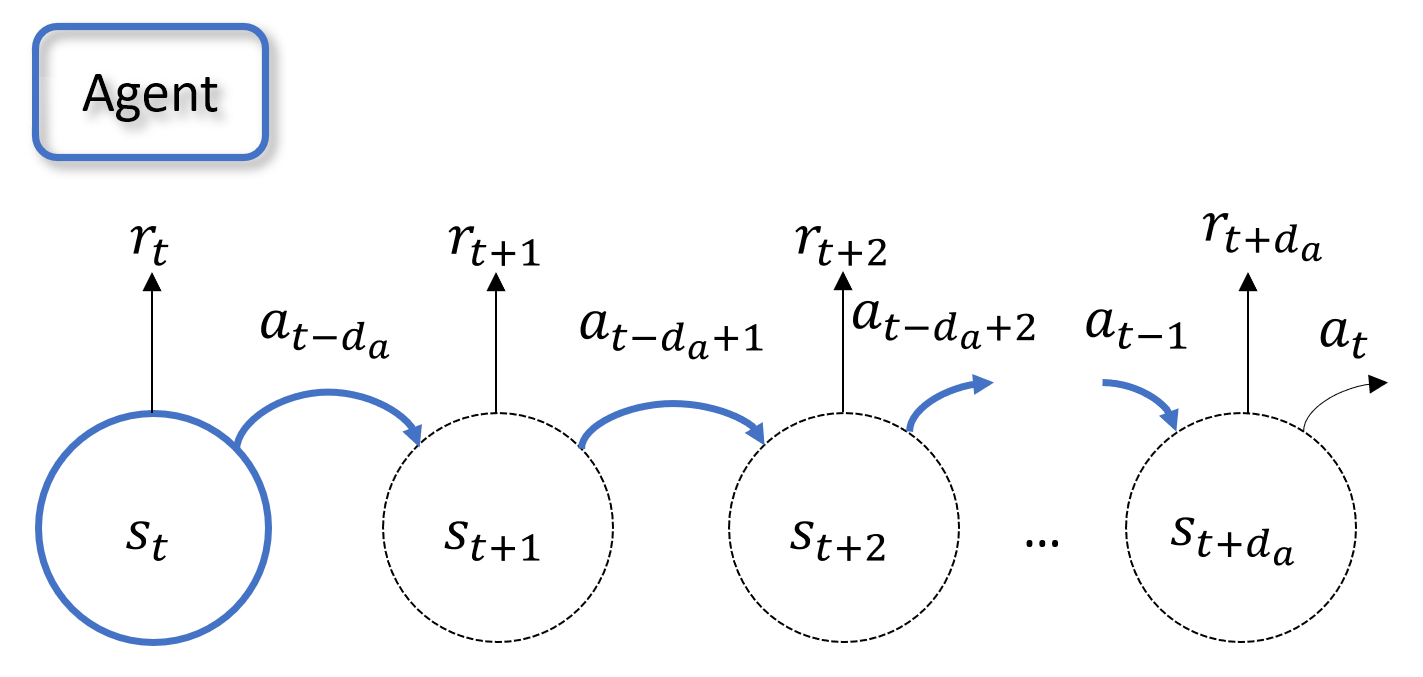
\includegraphics[width=11cm, keepaspectratio]{images/dmdp/augmented_i_a.png}
                    \caption{Augmented State $i_t^a$ is mapped onto the underlying DMDP process and it is highlighted in light blue. Reward delay is ignored for a clearer representation of the augmented state.}
                    \label{fig:augmented_i_a}
                \end{figure}
                \begin{figure}[t]
                    \centering
                    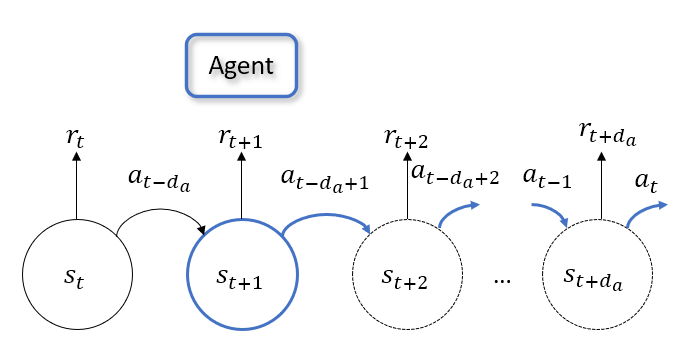
\includegraphics[width=11cm, keepaspectratio]{images/dmdp/augmented_i_a_next.png}
                    \caption{Augmented State $i_{t+1}^a$ is mapped onto the underlying DMDP and it is highlighted in light blue. Reward delay is ignored for a clearer representation of the augmented state.}
                    \label{fig:augmented_i_a_next}
                \end{figure}
                
                Again, the transition between augmented states is not the effect of the currently chosen action $a_t$, but rather of the action chosen $d_{a}$ steps before, $a_{t-d_{a}}$. This definition gives insight on how the newly formulated MDP works w.r.t. the previous DMDP framework. At a given timestep $t$, the Agent finds itself in an augmented state $i_t^{a} = \left( s_t, a_{t-d_{a}}, ..., a_{t-1} \right)$ and it chooses an action $a_t$. Action $a_{t-d_{a}}$ is then executed and as consequence  the Agent finds itself a new augmented state $i_{t+1}^{a} = \left( s_{t+1}, a_{t-d_{a}+1}, ..., a_{t-1}, a_{t} \right)$ with probability $p_a \left( i_{t+1}^a | i_t^a , a_t  \right)$ and collects a reward $r_t = \mathbf{R_{a}}\left( i_t, a_{t}, i_{t+1} \right)$. The new augmented state $i_{t+1}^{a}$ does not contain the executed action $a_{t-d{a}}$, since the information about it is already contained in $s_{t+1}$, and it adds the selected action $a_t$ at its "tail". From a pratical point of view, the sequence of actions contained in the augmented state are treated as a FIFO queue. Figure \ref{fig:augmented_i_a_next} shows the new augmented state $i_{t+1}^{a}$ as a comparison against $i_t^{a}$ shown in Figure \ref{fig:augmented_i_a}.
                With all the elements presented, the main result of \pcite{delay:execaugment} can now be stated in a complete and compact way in the following theorem:
            
                \begin{theorem}[DMDP Reduction for Execution Delay]
                    \label{th:dmdpexecred}
                    A Constantly Delayed MDP with execution and reward delay $\langle \mathbf{S}, \mathbf{A}, p, \mathbf{R}, 0, d_a, d_r \rangle$ is reducible to an undelayed augmented MDP $\langle \mathbf{I_a}, \mathbf{A}, p_a, \mathbf{R_a} \rangle$ with: 
                    \begin{itemize}[topsep=0.5em, partopsep=0.5em]
                        \setlength\itemsep{0em}
                        \item $\mathbf{I_{a}} \doteq \mathbf{S} \times \mathbf{A}^{d_a}$;
                        \item $p_a \left( i_{t+1}^a | i_t^a , a_t  \right) = p \left( s_{t+1} | s_t, a_{t-d_{a}} \right)$;
                        \item $\mathbf{R_{a}}\left( i_t, a_{t}, i_{t+1} \right) = \mathbf{R} \left( s_t, a_{t-d_{a}}, s_{t+1} \right)$.
                    \end{itemize}
                \end{theorem}
                
            \subsubsection{State Augmentation for Observation Delay}
                A similar result to Theoreom \ref{th:dmdpexecred} has been achieved in a different setting. Infact, \pcite{delay:obsaugment} showed that it is possible to reduce a Constantly Delayed MDP with observation and reward delay to an undelayed MDP. This objective can be achieved by definining all the elements of the undelayed MDP starting from the ones provided by the DMDP and it is a parallel derivation to the one presented in the last section. 
                
                \begin{figure}[t]
                    \centering
                    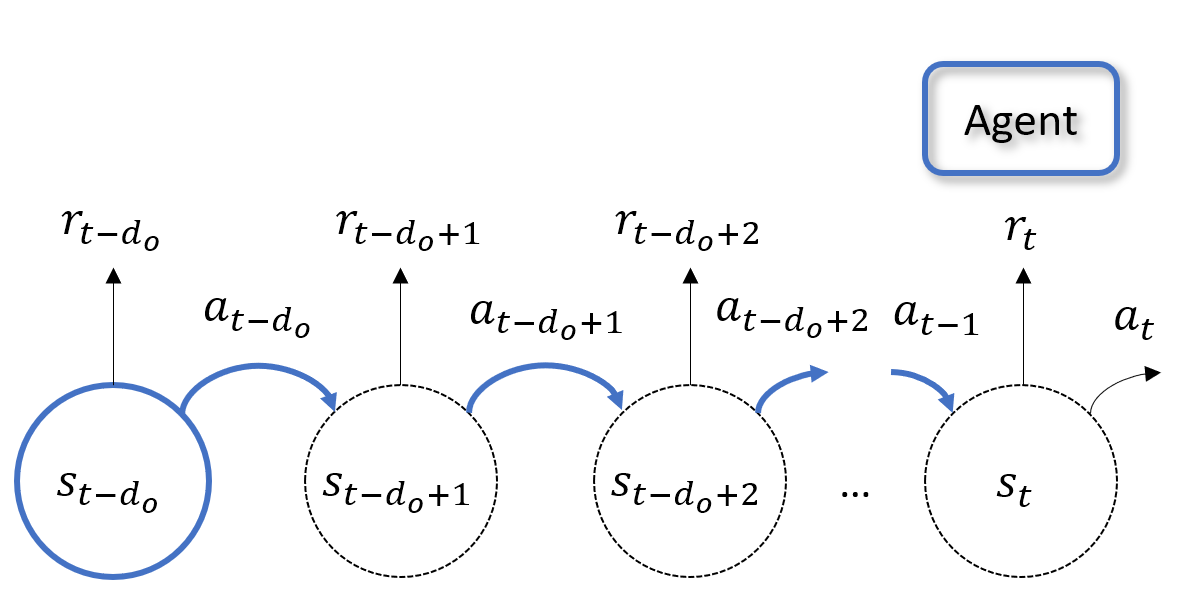
\includegraphics[width=11cm, keepaspectratio]{images/dmdp/augmented_i_o.png}
                    \caption{Augmented State $i_t^o$ is mapped onto the underlying DMDP process and it is highlighted in light blue. Reward delay is ignored for a clearer representation of the augmented state.}
                    \label{fig:augmented_i_o}
                \end{figure}
                \begin{figure}[t]
                    \centering
                    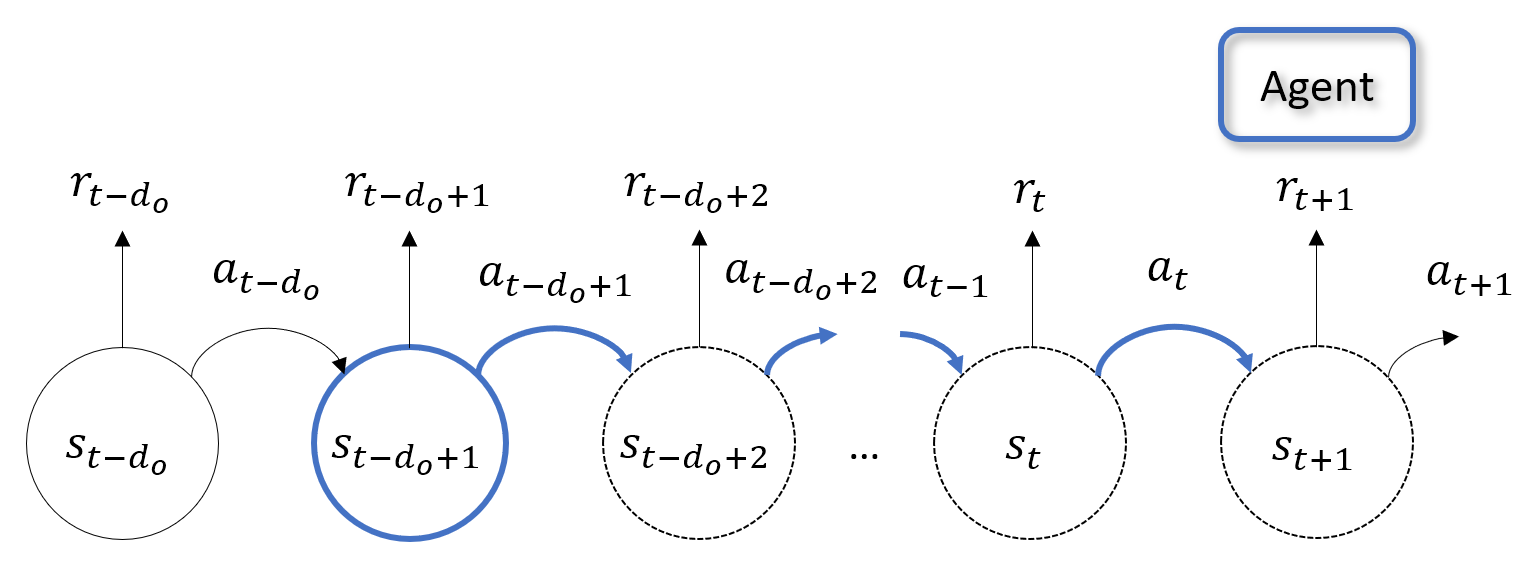
\includegraphics[width=13cm, keepaspectratio]{images/dmdp/augmented_i_o_next.png}
                    \caption{Augmented State $i_{t+1}^o$ is mapped onto the underlying DMDP and it is highlighted in light blue. Reward delay is ignored for a clearer representation of the augmented state.}
                    \label{fig:augmented_i_o_next}
                \end{figure}
                
                \begin{definition}[Augmented State Space $\mathbf{I_{o}}$]
                    \label{def:obsaugmentstate}
                    Given a Constantly Delayed MDP with observation and reward delay $\langle \mathbf{S}, \mathbf{A}, p, \mathbf{R}, d_o, 0, d_r \rangle$,
                    a new \textit{augmented} state space $\mathbf{I_{o}}$ can be defined as follows:
                    \[ \mathbf{I_{o}} \doteq \mathbf{S} \times \mathbf{A}^{d_o} \]
                    and each state $i^o_t$ is built from the elements of $\mathbf{S}$ and $\mathbf{A}$ in the following way:
                    \[ i_t^o= \left( s_{t-d_{o}}, a_{t-d_{o}}, a_{t-d_{o}+1}, ..., a_{t-1} \right)\]
                \end{definition}
                
                Figure \ref{fig:augmented_i_o} shows the augmented state $i_t^o$ is built starting from the DMDP elements. As in the previous section, the new augmented state space is built in such a way that each state contains all the information that can be available to the Agent.
                
                \begin{definition}[Augmented Reward function $\mathbf{R_o}$]
                    \label{def:obsaugmentreward}
                    Given a Constantly Delayed MDP with observation and reward delay $ \langle \mathbf{S}, \mathbf{A}, p, \mathbf{R}, d_o, 0, d_r \rangle$,
                    a new reward function $\mathbf{R_{o}}$ can be defined as follows:
                    \[ \mathbf{R_{o}}: \mathbf{I_{o}} \times \mathbf{A} \times \mathbf{I_{o}} \rightarrow \mathds{R}\]
                    and the values assigned by $\mathbf{R_{o}}$ can be computed in the following way:
                    \[ \mathbf{R_{o}}\left( i_t, a_{t}, i_{t+1} \right) = \mathbf{E} \left[ \mathbf{R} \left( s_t, a_t, s_{t+1} | i_t \right) \right] \]
                \end{definition}
                
                Differently from the previous section, the new augmented Reward function $\mathbf{R_o}$ is defined as the expected reward over all the possible current unobserved states $s_t$ knowing the current augmented state $i^o_t$, since the currently observed state $s_{t-d_{o}}$ is outdated and not involved in the current transition. 
                
                \begin{definition}(Augmented State-Transition Probability function $p_o$)
                    \label{def:obsaugmenttrans}
                    Given a Constantly Delayed MDP with execution and reward delay $\langle \mathbf{S}, \mathbf{A}, p, \mathbf{R}, d_o, 0, d_r \rangle$,
                    a new State-Transition Probability function $p_o$ can be defined as follows:
                    \[ p_o :  \mathbf{I_{o}} \times \mathbf{I_{o}} \times \mathbf{A} \rightarrow [0, 1]\]
                    and the probability values assigned by $p_o$ can be computed in the following way:
                    \[ p_o \left( i_{t+1}^o | i_t^o , a_t  \right) = p ( s_{t-d_{o}+1} | s_{t-d_{o}}, a_{t-d_{o}} ) \]
                \end{definition}                
                
                The process of transition between one augmented state $i^o_t$ and its successor $i^o_{t+1}$ is completely analogous to the process presented in the last section. The Agent starts from an augmented state $i^o_t = \left( s_{t-d_{o}}, a_{t-d_{o}}, a_{t-d_{o}+1}, ...,  a_{t-1}\right)$ and selects an action $a_t$. Then action $a_t$ is executed and the Agent finds itself in a new augmented state $i^o_{t+1} = \left( s_{t-d_{o}+1}, a_{t-d_{o}+1}, a_{t-d_{o}+2}, ...,  a_{t-1}, a_{t}\right)$ with probability $p_o \left( i_{t+1}^o | i_t^o , a_t  \right)$ and collects a new reward $\mathbf{R_{o}}\left( i_t, a_{t}, i_{t+1} \right)$. It is important to notice that in this case, the action chosen and the action that is actually executed are the same action, but the transition that the Agent experiences is consequence of the old action, $a_{t-d_{o}}$. The actions in the augmented state are treated as in a FIFO queue and the state is updated with the latest observed state. Figure \ref{fig:augmented_i_o_next} shows the next augmented state $i^o_{t+1}$ as a comparison against $i^o_t$ (Figure \ref{fig:augmented_i_o}).
                As in the previous section, with all the elements presented, \pcite{delay:obsaugment} result can be stated in a complete and more compact way in the following theorem:
                
                \begin{theorem}[DMDP Reduction for Observation Delay]
                    \label{th:dmdpobsred_v1}
                    A Constantly Delayed MDP with observation and reward delay $\langle \mathbf{S}, \mathbf{A}, p, \mathbf{R}, d_o, 0, d_r \rangle$ with $d_r \geq d_o$ is reducible to an undelayed augmented MDP $\langle \mathbf{I_o}, \mathbf{A}, p_o, \mathbf{R_o} \rangle$ with: 
                    \begin{itemize}[topsep=0.5em, partopsep=0.5em]
                        \setlength\itemsep{0em}
                        \item $\mathbf{I_{o}} \doteq \mathbf{S} \times \mathbf{A}^{d_o}$;
                        \item $p_o \left( i_{t+1}^o | i_t^o , a_t  \right) = p ( s_{t-d_{o}+1} | s_{t-d_{o}}, a_{t-d_{o}})$;
                        \item $\mathbf{R_{o}}\left( i_t, a_{t}, i_{t+1} \right) = \mathbf{E} \left[ \mathbf{R} \left( s_t, a_t, s_{t+1} | i_t \right) \right]$.
                    \end{itemize}
                \end{theorem}
                
                In this theorem, it is also expressed as an assumption that $d_r \geq d_o$. This is necessary due to the fact that the reward signal constitutes partial information about the transition that generated it and thus about the states that the transition involves. As stated in \pcite{delay:dmdp}, this assumption is sufficient to avoid that information about the reward signal does not reflects on the information about the augmented state, which would create a more complex interaction between delays.
                
            \subsubsection{Asynchronous Reward Collection}
                Before diving further into the Augmented Approach, an important intermediate result must be established in order to align the two augmentation processes presented in the last two sections. \pcite{delay:dmdp} refines the work of \pcite{delay:obsaugment} by introducing the concept of \textit{asynchronous reward collection}. It is shown and proved that a different and easier reward function can be used in the process of creating the Augmented MDP:
                \[ \mathbf{R_{o}}\left( i^o_t, a_{t}, i^o_{t+1} \right) = \mathbf{R}\left(s_{t-d_{o}}, a_{t-d_{o}}, s_{t-d_{o}+1} \right)\]
                For a more intuitive understanding, in Figure \ref{fig:augmented_i_o}, the next collected reward would be $r_{t-d_{o}+1}$. Thus, the reward signal perceived by the Agent is the actual delayed reward signal of the original DMDP. This allows for collecting each reward exactly once and in the correct order, albeit delayed, and given that distance in time-steps between two collected rewards is the same as the distance in time-steps between the two transitions that produced them, they are also discounted properly. This property is due to the constant nature of the delays in the original CDMDP. \color{red} Insert Proof? \color{black} \newline
                In light of this step forward, Theorem \ref{th:dmdpobsred_v1} can be reformulated including this additional result:
                
                \begin{theorem}[DMDP Reduction for Observation Delay]
                    \label{th:dmdpobsred_v2}
                    A Constantly Delayed MDP with observation and reward delay $\langle \mathbf{S}, \mathbf{A}, p, \mathbf{R}, d_o, 0, d_r \rangle$ with $d_r \geq d_o$ is reducible to an undelayed augmented MDP $\langle \mathbf{I_o}, \mathbf{A}, p_o, \mathbf{R_o} \rangle$ with: 
                    \begin{itemize}[topsep=0.5em, partopsep=0.5em]
                        \setlength\itemsep{0em}
                        \item $\mathbf{I_{o}} \doteq \mathbf{S} \times \mathbf{A}^{d_o}$;
                        \item $p_o \left( i_{t+1}^o | i_t^o , a_t  \right) = p ( s_{t-d_{o}+1} | s_{t-d_{o}}, a_{t-d_{o}})$;
                        \item $\mathbf{R_{o}}\left( i_t, a_{t}, i_{t+1} \right) = \mathbf{R}\left(s_{t-d_{o}}, a_{t-d_{o}}, s_{t-d_{o}+1} \right)$.
                    \end{itemize}
                \end{theorem}
                
                Thanks to this last addition, the augmentation process of a CDMDP affected by observation delay is completely aligned to the augmentation process of a CDMDP affected by execution delay. This allows for the derivation of the next results for the Augmented Approach.
            
            \subsubsection{Observation and Execution Delay Equivalency}
                \label{subsubs:delayeq}
                Further important steps towards unifying the Augmented Approach have been taken by \pcite{delay:dmdp}. It is stated and proved that Observation delays and Execution delays are equivalent from the perspective of the Agent and that their effect on the Augmented MDP are additive in such a way that it is possible to formulate an augmented MDP able to express the presence of both.
                \\\\
                The equivalence of observation and execution delay can be intuitively understood by observing Figure \ref{fig:augmented_i_a} and Figure \ref{fig:augmented_i_o}. In both situations, the augmented states $i^o_t$ and $i^a_t$ are constructed by using the same knowledge about the original DMDP and thus the Agent's decision-making process is based on the same notions about the Environment. The only difference between the two situations is the actual location of the Agent and thus the indexes that denotes states and actions, which is actually irrelevant to the Agent precisely because of the presence of delays. The same considerations can be made observing Figure \ref{fig:augmented_i_a_next} and Figure \ref{fig:augmented_i_o_next} and for all the pairs of future augmented states.
                \\\\
                Infact, it is easy to observe that Theorem \ref{th:dmdpexecred} and \ref{th:dmdpobsred_v2} are formally equivalent for $d_o = d_a$. CDMDPs $\langle \mathbf{S}, \mathbf{A}, p, \mathbf{R}, 0, d_a, d_r \rangle$ and $\langle \mathbf{S}, \mathbf{A}, p, \mathbf{R}, d_o, 0, d_r \rangle$ are also formally equivalent for $d_o = d_a$. Thus, even the resulting Augmented MDPs $\langle \mathbf{I_o}, \mathbf{A}, p_o, \mathbf{R_o} \rangle$ and $\langle \mathbf{I_a}, \mathbf{A}, p_a, \mathbf{R_a} \rangle$ are formally equivalent. While observation and execution delays may be consequence of different real world processes and entities, this means that they are actually perceived as the same concept, with the same consequences, for the MDP Agent that interacts in the Augumented MDP framework.
                \\\\
                \begin{figure}[t]
                    \centering
                    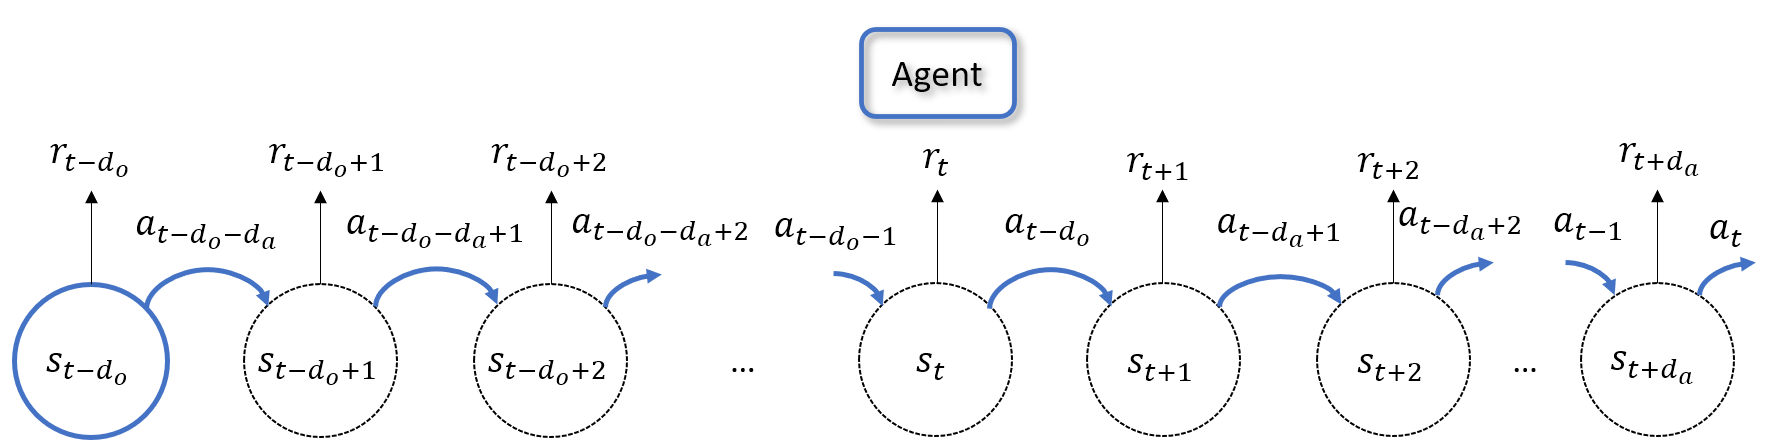
\includegraphics[width=15cm, keepaspectratio]{images/dmdp/augmented_i_ao.png}
                    \caption{Augmented State $i_t^{ao}$ is mapped onto the underlying DMDP process and it is highlighted in light blue. Reward delay is ignored for a clearer representation of the augmented state.}
                    \label{fig:augmented_i_ao}
                \end{figure}
                \begin{figure}[t]
                    \centering
                    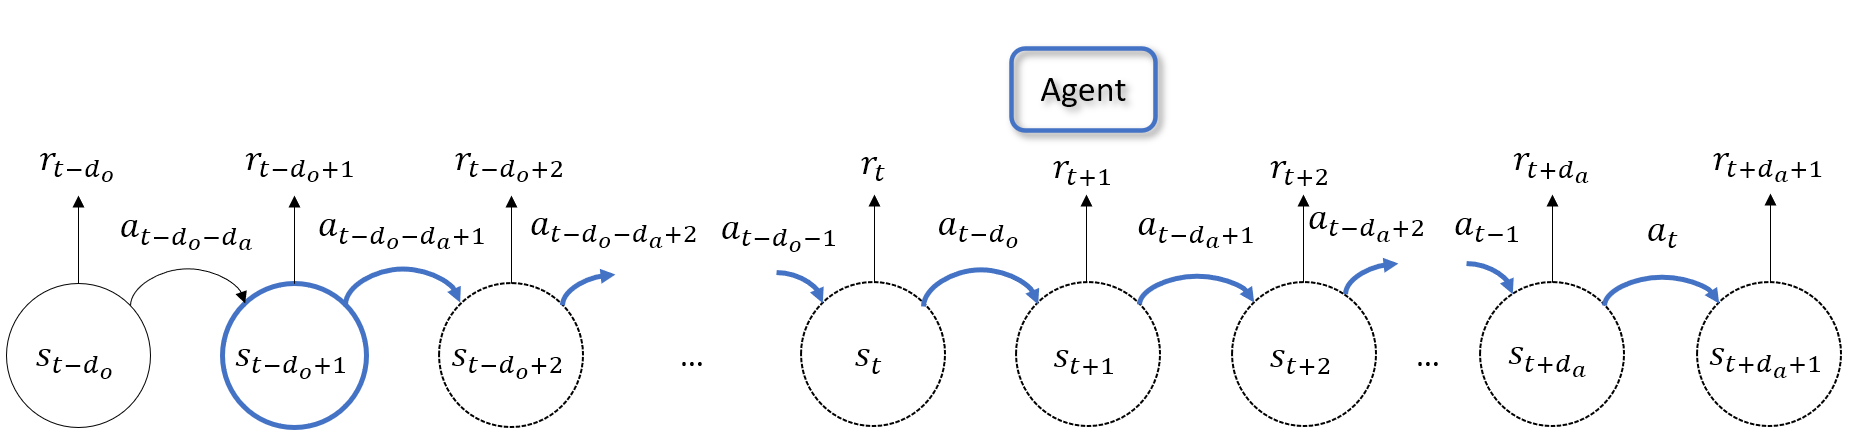
\includegraphics[width=15cm, keepaspectratio]{images/dmdp/augmented_i_ao_next.png}
                    \caption{Augmented State $i_{t+1}^{ao}$ is mapped onto the underlying DMDP and it is highlighted in light blue. Reward delay is ignored for a clearer representation of the augmented state.}
                    \label{fig:augmented_i_ao_next}
                \end{figure}
                Furthermore, from the equivalency of Observation and Execution delays it results that their combined effects on the Augmented MDP are additive when both are present. Supposing the presence of both observation $d_o \neq 0$ and execution delay $d_a \neq 0$, at each timestep $t$, the necessary information for optimal action selection is contained in 
                \[i_t = \left( a_{t-d_{o}-d_{a}}, a_{t-d_{o}-d_{a} +1}, ..., a_{t-d_{o}-1}, s_{t-d_{o}}, a_{t-d_{o}}, a_{t-d_{o}+1}, ..., a_{t-1} \right)\] Afterwards, the Agent selects the action $a_t$ and finds itself in a new augmented state: \[i_{t+1} = \left( a_{t-d_{o}-d_{a}+1}, a_{t-d_{o}-d_{a}+2}, ..., a_{t-d_{o}}, s_{t-d_{o}+1}, a_{t-d_{o}+1}, a_{t-d_{o}+2}, ..., a_{t-1}, a_{t}\right)\] with probability: \[p_{ao} \left( i_{t+1} | i_t, a_{t} \right) = p \left( s_{t-d_o+1} | s_{t-d_o}, a_{t-d_o-d_a} \right)\] and collecting a reward: \[\mathbf{R_{ao}}(i_t,a_t, i_{t+1}) = \mathbf{R}(s_{t-d_{o}}, a_{t-d_o-d_a}, s_{t-d_{o}+1})\] Figure \ref{fig:augmented_i_ao} and Figure \ref{fig:augmented_i_ao_next} shows augmented states $i_t$ and $i_{t+1}$ over the underlying Constantly Delayed MDP in the case where $d_o = d_a$. At last, in light of this result, the following complete theoreom can be stated:
                
                \begin{theorem}[CDMDP Reduction]
                    \label{th:dmdpred}
                    A Constantly Delayed MDP $\langle \mathbf{S}, \mathbf{A}, p, \mathbf{R}, d_o, d_a, d_r \rangle$ with $d_r \geq d_o$ is reducible to an undelayed augmented MDP $\langle \mathbf{I_d}, \mathbf{A}, p_d, \mathbf{R_d} \rangle$ with: 
                    \begin{itemize}[topsep=0.5em, partopsep=0.5em]
                        \setlength\itemsep{0em}
                        \item $\mathbf{I_d} \doteq \mathbf{S} \times \mathbf{A}^{d_o+d_a}$;
                        \item $p_d \left( i_{t+1} | i_t, a_{t} \right) = p \left( s_{t-d_o+1} | s_{t-d_o}, a_{t-d_o-d_a} \right)$;
                        \item $\mathbf{R_d}(i_t,a_t, i_{t+1}) = \mathbf{R}(s_{t-d_{o}}, a_{t-d_o-d_a}, s_{t-d_{o}+1})$.
                    \end{itemize}
                \end{theorem}
                
                As in theorem \ref{th:dmdpobsred_v2}, the assumption $d_r \geq d_0$ is used in order to avoid situations in which the reward signal provides information about yet unobserved states. 
            
                
            \subsubsection{Approach Advantages: Markov Property and wide Applicability}
                In Section \ref{subs:markovmdp}, it is stated that the presence of delay actively hinders the Markov Property (Definition \ref{def:markov}). While the state itself still represents a sufficient statistic for the trajectory drawn before it, the fact that the Agent must plan its actions using outdated states w.r.t the actions consists in a direct violation of the Markov Property, which in turn is the foundation of the MDP framework itself, allowing for optimal action planning at each time-step. \newline
                One of the strongest advantages of the Augmented Approach is that the augmented MDP that is formulated from the original CDMDP retains the Markov Property. Infact, the Agent that interacts in the augmented MDP framework is reasoning upon augmented states that are built by joining together all the information that is available for optimal action planning. Furthermore, from the point of view of the Agent interacting with an augmented MDP, there is no notion of delay. \newline
                Even further, the Agent is interacting with a standard MDP framework: the Agent is not interested in how the augmented state is built and each action inserted along with the last observed state is seen as new dimensions for each augmented state. Thus, any algorithm developed for interacting in the MDP framework can be used to learn the augmented MDP without any restriction. This allows state of the art algorithm to be tested directly on a delay setting without further modification to the algorithms themselves, resulting in a very large applicability of the approach. However, these benefits also comes with substantial costs.
                
            \subsubsection{Approach Disadvantages: Computational Complexity}
                While the Augmented Approach leads to a sound and complete framework that enables the possibility of acting optimally in a delayed environment, it also implies a major change in the state space in order to retain the Markov assumption. Infact, augmented states are not only containing information about the environment itself, but in order to recover lost information due to delay, a sequence of actions chosen by the Agent is also added. \newline
                From the implementation point of view, the added actions function just as new dimensions for the vector or tensor that represents the augmented state, which will be larger than the original state and grows larger linearly in the number of delay time-steps. Larger states usually indicate an inherently more difficult setting to learn, leading to higher variance and thus a less clear cause-effect transition. From the theoretical complexity point of view, the Augumented State Space $\mathbf{I_d}$ is much larger than the correspective State Space $\mathbf{S}$. Infact, for each state $s_t$ belonging to the original state space $\mathbf{S}$, there exist a set of augmented states $i_t$ that are built from $s_t$ as a last observed state and all the possible sequences of actions of lenghts $d_o+d_a$ that are planned to be executed afterwards. This is also evident from the definition of the augmented state space: $\mathbf{I_d} \doteq \mathbf{S} \times \mathbf{A}^{d_o+d_a} \doteq \mathbf{S} \times \mathbf{A}_{1} \times \mathbf{A}_{2} \times ... \times \mathbf{A}_{d_o+d_a}$. Intuitively, the need of taking into consideration all the possible sequences of actions leads to an exponential growth in the number of delay time-steps. This intuition is taken into action in \pcite{delay:mbs}, in which a formal proof of the following theorem is provided:
                
                \begin{theorem}[Augmented State Space Complexity]
                    \label{th:dmdpobscomplexity}
                    The Augmented State Space $\mathbf{I_d}$'s cardinality of an Augmented MDP $\langle \mathbf{I_d}, \mathbf{A}, p_d, \mathbf{R_d} \rangle$ derived from a Constantly Delayed MDP $\langle \mathbf{S}, \mathbf{A}, p, \mathbf{R}, d_o, d_a, d_r \rangle$ has a lower bound of \[ | \mathbf{I_d} | = \Omega \left( | \mathbf{A}^{d_o + d_a} | \right) \]
                \end{theorem}
                
                The symbol $\Omega$ denotes the Big O notation. This result needs to be coupled with a more classical theorem that states that a MDP with fixed discount factor is solvable in polynomial time w.r.t. the State Space cardinality $| \mathbf{I_d} |$. Thus, being the State Space cardinality exponential in the length of delay $d = d_o + d_a$, the Augmented MDP can be solved in exponential time w.r.t. the length of delay $d = d_o + d_a$. This is inherently due to how the Augmented State Space $\mathbf{I_d}$ is built and it has a strong effect on applicability, since CDMDPs with relatively small delays may already be intractable in practice with the Augmented Approach.
                
            \subsubsection{Stochastically Delayed MDP Augmentation}
                \label{subsubs:sdmdpaug}
                In the previous paragraphs of this section, the attention is posed on the CDMDP framework due to its more intuitive and less convoluted structure, that allows for presenting results in a straightforward approach. Nonetheless, equivalently important results have been derived on the Stochastically Delayed MDP framework. Infact, \pcite{delay:dmdp} also provides completely parallel results which allows for applying the Augmented Approach also to SDMDP, with some minor but important differences.
                \\\\
                \textbf{State Space Augmentation} needs to take into account the fact that the Agent does not receive an observation at each time-step due to the randomness of the delay. Thus the number of dimensions of each augmented state cannot be fixed: the number of actions that occurs between one state observation and the next is not fixed, but they all must be included in order to retain the Markov Property and optimal action selection. Each augmented state is built as follows from the original SDMDP states:
                \[ i_t = \left( s_{t-d_o}, t-r, a_{t-o}, ..., a_{t-1} \right) \]
                where the execution delay $d_a$ is equal to 0 for simplicity of representation and r is the number of timesteps from the last observation. Note that in this context, $d_o$ is not the constant delay but the delay sampled by the stochastic process $d_o(t)$ at time-step $t-d_o$. 
                \\\\
                It is important to highlight that a variable-length augmented state $i_t$ also constitutes a challenge from the algorithm's implementation perspective, since most of the algorithms that have been design to solve MDPs have also been design to exploit fixed-length states.
                \\\\
                An important assumption made in \pcite{delay:dmdp} is that state $s_{t+1}$ can be observed only after the observation of state $s_t$, which is coupled with the usual constraint $d_o > d_r$ to ensure that the reward result of the $t+1$ timestep can be collected only after the observation of the state $s_{t+1}$, in order not to reveal any conflicting information about the state itself. These assumptions have substantial consequences upon the \textbf{Augmented State-Transition probability function}, which forces the augmented state to grow indefinitely large with time.
                \begin{definition}(Augmented State-Transition function $p_d$ (SDMDP))
                    \label{def:sdmdpaugtrans}
                    \[ p_d \left( i_{t+1} | i_t, a_t \right) =  
                        \begin{cases} 
                            p \left( s_{t-d_o+1} | s_{t-d_o}, a_{t-d_o} \right) q\left(r\right) & if \; i_{t+1} = i \\
                            1 - q\left(r\right) & if \; i_{t+1} = i'\\
                        \end{cases}
                    \]
                    where:
                \end{definition}
                \begin{itemize}[topsep=0.5em, partopsep=0.5em]
                    \setlength\itemsep{0em}
                    \item $q(r) = \mathds{P}\left( d_o(t) = r \right) /\; \mathds{P}\left( d_o(t) \geq r \right) $ represents the probability that the new state $s_{t-d_o+1}$ is observed in the next timestep $t+1$, given that currently observed state $s_{t-d_o}$ has been first observed $t-r$ timesteps before.
                    \item $i = \left( s_{t-d_o+1}, t+1, a_{t-d_o+1}, ..., a_{t}\right)$ is the augmented state the Agent will find itself in if $s_{t-d_o+1}$ is observed at timestep $t+1$.
                    \item $i' = \left( s_{t-d_o}, t-r+1, a_{t-o}, ..., a_{t-1}, a_{t} \right)$  is the augmented state the Agent will find itself in if no new state is observed at timestep $t+1$.
                \end{itemize}
                This definition of State-Transition Probability function implies that, at each timestep, the augmented state's dimensions can either remain constant or grow exactly by 1. In turn, this means that the augmented state will grow indefinitely with time if the Agent is not halted in order to wait for new observations without acting further, so to shrink the Augmented State to an acceptable size.
                \\\\
                The \textbf{Augmented Reward Function} also needs to take into account that the number of steps between observations is not constant and thus the reward signal needs to be assigned to a transition happened a variable number of steps before and avoid repeating the last reward signal at each timestep in which no new state is observed. Suppose the current augmented state is $i_t = \left( s_{t-d_o}, t-r, a_{t-o}, ..., a_{t-1} \right)$ and that state $s_{t-d_o+1}$ is the next observed state, then the Reward function is defined as:
                \begin{definition}(Augmented Reward Function $\mathbf{R_d}$ (SDMDP))
                    \label{def:sdmdpaugrew}
                    \[ \mathbf{R_d} \left( i_t, a_t, i_{t+1} \right) =  
                        \begin{cases} 
                            \mathbf{R} \left( s_{t-d_o}, a_{t-d_o}, s_{t-d_o+1} \right) & if \; i_{t+1} = i \\
                            0 & if \; i_{t+1} = i'\\ 
                        \end{cases}
                    \]
                where $i$ and $i'$ are defined as in Definition \ref{def:sdmdpaugtrans}.
                \end{definition}
                
                At last, the effect of the presence of Execution Delay $d_a(t)$ is completely analogous to the CDMDP framework: 
                \begin{itemize}[topsep=0.5em, partopsep=0.5em]
                    \setlength\itemsep{0em}
                    \item Execution and Observation delays are equivalent from the point of view of the Agent that is interacting in the Environment.
                    \item Execution and Observation delays have an additive effect on the when present together (as explained in Section \ref{subsubs:delayeq}).
                \end{itemize}
                Taking into account all the definition given so far, a complete theorem on SDMDP reduction to an undelayed Augmented MDP can be stated as a last result:
                \begin{theorem}[SDMDP Reduction]
                    \label{th:sdmdpred}
                    A Stochastically Delayed MDP $\langle \mathbf{S}, \mathbf{A}, p, \mathbf{R}, d_o(t), d_a(t), d_r(t) \rangle$ is reducible to an undelayed augmented MDP $\langle \mathbf{I_d}, \mathbf{A}, p_d, \mathbf{R_d} \rangle$ with: 
                    \begin{itemize}[topsep=0.5em, partopsep=0.5em]
                        \setlength\itemsep{0em}
                        \item $\mathbf{I_{d}} \doteq \Big\{ i_t = \left( a_{t-d_{o}(t)-d_{a}(t)}, ..., s_{t-d_{o}(t)}, t-r(t), a_{t-d_{o}(t)}, ..., a_{t-1} \right), \; \forall t \in \mathbf{T} \Big\}$
                        \item $p_d \left( i_{t+1} | i_t, a_t \right) \doteq  
                                    \begin{cases} 
                                        p \left( s_{t-d_o+1} | s_{t-d_o}, a_{t-d_o-d_a} \right) q\left(r\right) & if \; i_{t+1} = i \\
                                        1 - q\left(r\right) & if \; i_{t+1} = i'\\
                                    \end{cases}$
                        \item $\mathbf{R_d} \left( i_t, a_t, i_{t+1} \right) \doteq  
                                    \begin{cases} 
                                        \mathbf{R} \left( s_{t-d_o}, a_{t-d_o-d_a}, s_{t-d_o+1} \right) & if \; i_{t+1} = i \\
                                        0 & if \; i_{t+1} = i'\\ 
                                    \end{cases}$
                    \end{itemize}
                    where:
                    \begin{itemize}[topsep=0.5em, partopsep=0.5em]
                        \setlength\itemsep{0em}
                        \item $i = \left( a_{t-d_{o}-d_{a}+1}, ..., s_{t-d_o+1}, t+1, a_{t-d_o+1}, ..., a_{t}\right)$, in which $d_o$ and $d_a$ are delays sampled by the stochastic processes $d_o(t)$ and $d_a(t)$;
                        \item $i' = \left( a_{t-d_{o}-d_{a}}, ..., s_{t-d_o}, t-r+1, a_{t-o}, ..., a_{t-1}, a_{t} \right)$, in which $d_o$ and $d_a$ are delays sampled by the stochastic processes $d_o(t)$ and $d_a(t)$;
                    \end{itemize}
                \end{theorem}
        
        \newpage
        \subsection{Memoryless Policy Approach}
            \label{subs:memorylessapproach}
            The Memoryless Policy approach aims to cope with the presence of delays without incurring into excessive computional complexity, by not including or by partially including the notion of delays during the learning process of the Agent, thus aiming to suboptimal performances unless specific proofs about the possibility to reach optimal behaviour are stated.
            
            \subsubsection{Basic Approach}
                The basic approach is constituted by applying already existing algorithms to a CDMDP, ignoring the presence of delays. This entails that the CDMDP $\langle \mathbf{S}, \mathbf{A}, p, \mathbf{R}, d_o, d_a, d_r \rangle$ is treated by the Agent as an undelayed MDP $\langle \mathbf{S}, \mathbf{A}, p, \mathbf{R} \rangle$. At each timestep $t$, the Agent find itself in a state $s_t$, selects an action $a_t$ and observes a new state $s_{t+1}$ receiving a reward $r_t$, without being aware of the following facts:
                \begin{itemize}[topsep=0.5em, partopsep=0.5em]
                        \setlength\itemsep{0em}
                        \item $s_t$ is the old state $s_{t-d_o}$;
                        \item $a_t$ is executed in $d_a$ steps;
                        \item $r_t$ is the old reward $r_{t-d_r}$;
                        \item the current transition from $s_t$ to $s_{t+1}$ is not consequence of action $a_t$, but of action $a_t-d_a$.
                \end{itemize}
                
                In practice, this means that the decision-maker is basing the action selection only on the most recent observation. Even if the Environment could provide an augmented state $i_t = \left( a_{t-d_{o}-d_{a}}, ..., a_{t-d_{o}-1}, s_{t-d_{o}}, a_{t-d_{o}}, ..., a_{t-1} \right)$, which comprises all the needed information for optimal decision-making, the Agent's policy $\pi$ is a function only of the state $s_{t-d_{o}}$:
                
                \[ \pi'(i_t) = \pi(s_{t-d_o}) \]
                
                Infact, the term "Memoryless" is borrowed from the POMDP research, where it is used to describe policies that are functions of the observation $o_t$ the Agent perceives and not of some learnt representation of the hidden state (see Section \ref{sota:pomdp}).
                \\\\
                While the Agent is void of information about the effect of delays on its interaction with the Environment, it does not need to cope with an exponential state space such in the case of the Augmented approach (Theorem \ref{th:dmdpobscomplexity}) or to learn a model representation of the CDMDP (\color{red}insert reference on ModelBased Approach\color{black}), resulting in a much simpler and faster approach. As explained in the Introduction, computational time is an unavoidable source of delays in a real world application, thus the Memoryless approach could provide a benefit in cases in which fast computations are a strong requirement.
                \\\\
                In order to properly introduce an important result for the Memoryless approach in the next section, two classic algorithms for solving MDPs presented here: SARSA (\pcite{sarsa}) and Q-Learning (\pcite{qlearning}). They are both contained in the larger set of algorithms called Temporal Difference (TD) learning methods and they both aims at estimating the action-value function $q(s,a)$, also called q-function, in an online learning setting. After the conclusion of each time-step $t$, the Agent updates its values of $q(s,a)$ by exploiting knowledge on the concluded transition $s_t, a_t, r_{t+1}, s_{t+1}, a_{t+1}$ with the following update rules:
                \begin{align*}
                    q(s_t, a_t) &\leftarrow q(s_t, a_t) + \alpha \delta_{TD, t}\\
                    \delta_{SARSA, t}    &= r_{t+1} + \gamma q(s_{t+1}, a_{t+1}) - q(s_t, a_t)\\
                    \delta_{Q, t}        &= r_{t+1} + \gamma \max_{a'} q(s_{t+1}, a') - q(s_t, a_t)\\
                \end{align*}
                where $\leftarrow$ denotes the update over the same value $q(s_t, a_t)$; $\gamma$ is the discount factor and $0 \leq \alpha \leq 1$ is the learning rate, which determines the strength of each single update. The update rule makes SARSA an on-policy learning algorithm, since the q-function is updated using the currently learnt q-function values and thus denoting the same policy that is being used for drawing the trajectory; while Q-Learning is an off-policy learning algorithm, since its updates are based on the optimal q-function and thus on the optimal policy, which is different from the policy used to draw trajectories. \newline
                At each step $t$, action $a_t$ is usually chosen by either following the greedy policy or an $\epsilon$-greedy policy:
                \begin{align*}
                    \pi_{greedy}(s_t) &= \argmax_{a'}q(s_t, a')\\
                    \pi_{\epsilon -greedy}(s_t) &= 
                                    \begin{cases} 
                                        \argmax_{a'}q(s_t, a') & with \; probability \; 1 - \epsilon \\
                                        random & with \; probability \; \epsilon \\ 
                                    \end{cases}
                \end{align*}
                where $\pi_{\epsilon -greedy}$ ensures a certain degree of exploration while drawing trajectories in the environment, which can be tuned by changing the \textit{exploration rate} $0 \leq \epsilon \leq 1$, lowering or increasing the chances to act randomly and thus not exploiting the knowledge learnt so far.
                \\\\
                Substantial improvements have been reached by applying \textit{Eligility Traces} (\pcite{temporaldifference}) to the Temporal Difference learning set of methods, bringing the development of new versions of the presented algorithms: SARSA($\lambda$) (\pcite{sarsalambda}) and Q($\lambda$)(\pcite{qlearning}). These methods differ from their predecessors in their update rule, which includes the eligibility traces in order to keep track of the contributions of recent transitions w.r.t. the current one:
                \begin{align*}
                    q_{t+1}(s, a) &\leftarrow q_{t}(s, a) + \alpha \delta_{TD, t} e_t(s, a)\\
                    \delta_{SARSA, t}    &= r_{t+1} + \gamma q(s_{t+1}, a_{t+1}) - q(s_t, a_t)\\
                    \delta_{Q, t}        &= r_{t+1} + \gamma \max_{a'} q(s_{t+1}, a') - q(s_t, a_t)\\
                    e_{t}(s,a) &= 
                            \begin{cases} 
                                1 & if \; s = s_t \; \wedge \; a = a_t \\
                                \gamma \lambda e_{t-1}(s, a) & otherwise \\ 
                            \end{cases}
                \end{align*}
                where the update is now involving all $s \in \mathbf{S}$ and all $a \in \mathbf{A}$ and with $ 0 \leq \lambda \leq 1$, usually treated as an hyperparameter of the method to be tuned. At the beginning of each episode, the eligibility trace vector $e_t$ is initialized at 0. At each step $t$, the action-value function $q$ is updated for all possible couples $(s, a)$. If $(s, a) = (s_t, a_t)$, the update is "full", as for SARSA or Q-Learning, since the eligiblity trace is set at 1. Otherwise, the eligibility traces is set to its previous value $e_{t-1}$ weighted by the $\gamma \lambda$ factor, causing the updates to fade in time. This ensures that the benefits or drawbacks of choosing action $a_t$ in state $s_t$ are propagated back "in time" to the previous transitions. SARSA($\lambda$) and Q($\lambda$) have been shown to converge faster than SARSA and Q-Learning, thus constituting overall better methods.
                \\\\
                As pointed out at the beginning of this section, the Memoryless approach can be applied to any existing algorithm, which will produce an Agent that acts unaware of the delay. Both SARSA($\lambda$) and Q($\lambda$) can be used to test this approach against the others and, infact, SARSA($\lambda$) has been chosen as one of the performance basilines for this research and its results are shown in Chapter \ref{chp:results}. The complete algorithm is presented in Algorithm \ref{algo:sarsalambda}.
                
                \begin{algorithm}[t]
                    \SetAlgoLined
                    \KwResult{Optimal Action-value function: $q_{*}(s,a)$ }
                    Initialize the action-value function $q(s,a)$ arbitrarility or at 0\;
                    Initialize the values of the Discount factor $\gamma$ and eligibility traces $\lambda$\;
                    Initialize the eligibility traces $e(s,a)=0$\;
                    Initialize number of episodes, $N$, and $n=0$\;
                    \While{$n \leq N$}{
                        Initialize the first state of the episode, $s_0$\;
                        Initialize the first action of the episode, $a_0$\;
                        Initialize the number of steps of the episode, $T$, and $t=0$\;
                        \While{$t \leq T$}{
                            Agent executes action $a_t$\;
                            Agent observes state $s_{t+1}$\;
                            Agent receives reward $r_{t+1}$\;
                            Agent selects the next action $a_{t+1} = \pi_{\epsilon -greedy}(s_{t+1})$\;
                            Compute: $\delta \leftarrow r_{t+1} + \gamma q(s_{t+1},a_{t+1}) - q(s_t, a_t)$\;
                            Set Eligibility Traces: $e(s_t, a_t) \leftarrow e(s_t, a_t) + 1$\;
                            \For{$s \in \mathbf{S} \wedge a \in \mathbf{A}$}{
                                $q(s, a) \leftarrow q(s, a) + \alpha \delta e(s, a)$\;
                                $e(s, a) \leftarrow \gamma \lambda e(s, a) $\;
                            }
                            Update $t=t+1$\;
                        }
                        Update $n=n+1$\;
                    }
                    \caption{SARSA($\lambda$)}
                    \label{algo:sarsalambda}
                \end{algorithm}
            
            
            
            \subsubsection{DSARSA and DQ-Learning}
                \pcite{delay:memoryless} propose a step forward for SARSA($\lambda$) and Q($\lambda$), developing two new algorithms in order to apply Temporal Difference learning to the setting of Execution Delay. As stated in Section \ref{subsubs:delayeq}, Observation and Execution delays are functionally equivalent for the Agent and thus the Execution delay setting does not incur into loss of generality w.r.t. the complete delay setting. 
                \\\\
                The new algorithms are called dSARSA($\lambda$) and dQ($\lambda$) and constitute an evolution of SARSA($\lambda$) and Q($\lambda$) respectively, by incorporating partial knowledge on the presence of the delay within the action-value function's update while retaining the advantages of the application of eligibility traces. Assuming constant delay of $d = d_a$ timesteps, the new algorithms apply the following update rule:
                \begin{align*}
                    q_{t+1}(s_t, a_{t-d}) &\leftarrow q_{t}(s_t, a_{t-d}) + \alpha \delta_{TD, t} e_t(s_t, a_{t-d})\\
                    \delta_{SARSA, t}    &= r_{t+1} + \gamma q(s_{t+1}, a_{t-d+1}) - q(s_t, a_{t-d})\\
                    \delta_{Q, t}        &= r_{t+1} + \gamma \max_{a'} q(s_{t+1}, a') - q(s_t, a_{t-d})\\
                    e_{t}(s,a) &= 
                            \begin{cases} 
                                1 & if \; s = s_t \; \wedge \; a = a_{t-d} \\
                                \gamma \lambda e_{t-1}(s, a) & otherwise \\ 
                            \end{cases}
                \end{align*}
                
                \begin{algorithm}[t]
                    \SetAlgoLined
                    \KwResult{Action-value function: $q_{\pi}(s,a)$}
                    Initialize the action-value function $q(s,a)$ arbitrarility or at 0\;
                    Initialize the values of the Discount factor $\gamma$ and eligibility traces $\lambda$\;
                    Initialize the eligibility traces $e(s,a)=0$\;
                    Initialize number of episodes, $N$, and $n=0$\;
                    \While{$n \leq N$}{
                        Initialize the first state of the episode, $s_0$\;
                        Initialize the first actions of the episode, $a_0, ..., a_d-1$\;
                        Initialize the number of steps of the episode, $T$, and $t=0$\;
                        \While{$t \leq T$}{
                            Agent executes action $a_{t+d}$\;
                            Agent observes state $s_{t+1}$\;
                            Agent receives reward $r_{t+1}$\;
                            Agent selects the next action $a_{t+d+1} = \pi_{\epsilon -greedy}(s_{t+1})$\;
                            Compute: $\delta \leftarrow r_{t+1} + \gamma q(s_{t+1},a_{t-d+1}) - q(s_t, a_{t-d})$\;
                            Set Eligibility Traces: $e(s_t, a_{t-d}) \leftarrow e(s_t, a_{t-d}) + 1$\;
                            \For{$s \in \mathbf{S} \wedge a \in \mathbf{A}$}{
                                $q(s, a) \leftarrow q(s, a) + \alpha \delta e(s, a)$\;
                                $e(s, a) \leftarrow \gamma \lambda e(s, a) $\;
                            }
                            Update $t = t + 1$\;
                        }
                        Update $n=n+1$\;
                    }
                    \caption{dSARSA($\lambda$)}
                    \label{algo:dsarsalambda}
                \end{algorithm}                
                
                The major difference with the classic algorithms is the presence of the "shifted" action within the update. In SARSA($\lambda$) and Q($\lambda$) the reward collected in a transition $(s_t, a_t, r_{t+1}, s_{t+1}, a_{t+1})$ is implicitly assigned to the tuple $(s_t, a_t, s_{t+1})$, but in presence of delays this constitutes a credit-assignment issue, since the Agent is never able to assign the reward to the correct tuple. dSARSA($\lambda$) and dQ($\lambda$) aim to solve this issue by assuming the delay is known and applying the action-value function update using the $d-step$ old action $a_{t-d}$ rather than the last chosen action $a_t$.\newline
                However, when the Agent selects action $a_t$, the execution is still delayed by $d$ steps and this is the reason why knowledge about delay is only partially considered from the point of view of the Agent. Furthermore, the delayed execution of actions is the main reason that cause convergence proofs about SARSA($\lambda$) and Q($\lambda$) not to hold anymore in the case of dSARSA($\lambda$) and dQ($\lambda$), since the delayed execution forbids the policy from being greedy in the limit of infinite exploration (GLIE): the action $a_t$ can be chosen greedily by the agent, but the state $s_{t+d}$ in which it will be actually executed is different from the state $s_t$ used to select them greedily. 
                \\\\
                DSARSA($\lambda$) has been chosen as a memoryless approach's algorithm to provide a baseline for this research: its results are presented in Chapter \ref{chp:results} and its complete algorithm is presented in Algorithm \ref{algo:dsarsalambda}.
                
            \subsubsection{Eligibility Traces and Partial Observability}
                In Section \ref{subs:pomdp}, a first conceptual point of contact between the POMDP and DMDP frameworks is established. Here, a more practical similarity between the two framework is discussed: the use of Eligibility Traces as a mitigation for partial observability or delayed observation/execution. \newline
                Similarly to \pcite{delay:memoryless}, \pcite{pomdp:eligibilitytraces} supports the use of memoryless algorithm such as SARSA($\lambda$) in partially observable environment as a decent, less computationally expensive, alternative to other model based approaches, which are inherently more expensive due to the burden of learning a representation of the current unobserved state. In particular, the presence of the eligibility traces enables a more correct credit-assignment process during the Agent training, which would not be possible otherwise. Infact, the major challenge in learning POMDP is that a given observation $o_t$ can result from several hidden states $s_t$ and choosing the same action $a_t$ may yield very different consequences, i.e. collecting different rewards $r_t$ from the same pair $(o_t, a_t)$. This ambiguity is unexplainable by the Agent which has only access to the same observation $o_t$ each time. With eligibility traces, this issue is mitigated: each pair $(o_t, a_t)$ is not only evaluated using the immediate reward $r_t$, but also by the sum of weighted future updates due to the rest of the pairs that characterize the trajectory. The evaluation of each pair $(o_t, a_t)$ is linked to the trajectory the follows it rather than the immediate reward $r_t$, reducing the "amount" of ambiguity from the point of view of the Agent. \newline
                In case of DMDP, the benefits from applying eligibility traces are similar. For example, in case of execution delay $d_a$, the major challenge is the immediate reward $r_t$ is assigned to the pair $(s_t, a_t)$, while it is actually the consequence of the pair $(s_t, a_{t-d_a})$. With eligibility traces, the immediate reward $r_t$ also have a direct impact in the action-value function update of the past trajectory, which also contains the correct action $a_{t-d_a}$. This is the reason why such a classical algorithm like SARSA($\lambda$) is interesting to be used as a baseline for research in DMDP.
        
            \subsubsection{Memoryless Approach for Stochastic Delays}
                Since the Memoryless approach is based on learning memoryless policies, it does not provide a specific general formalization for the presence stochastic delays. Thus, the limitations about learning in a stochastically delayed environment are completely algorithm-dependent. For example, SARSA($\lambda$) is "natively" compatible with learning in an environment with stochastic delays, since the Agent is aware only of the last observed state, which is always available no matter the kind and amount of delay at each step. Instead, dSARSA($\lambda$) has been designed to cope with constant delays and the Agent expects to know a fixed time-steps amount in order to re-align the delayed actions with the correspondent state. Thus, this algorithm would need to be adapted to re-align states and actions dinamically, expecting a different amount of delay steps at each time-step of the trajectory. \newline
            
        \newpage
        \subsection{Model-Based Approach}
            
            % Section Structure:
            %   - General Approach:
            %       - Keep already done general explanation
            %       - Model Based Simulation
            %       - Two Papers on Methods 
            %   - POMDP Literature:
            %       - First Paper
            %       - Second Paper
            %   - Advantages and Disadvantages + Stochastic Delays
        
            \label{subs:modelbasedapproach}
            The Model-Based approach searches for a middle ground approach between Memoryless Policies and Augmented MDPs, dividing the learning process in two different steps: learning the underlying MDP transition function, thus being able to provide a representation of the current unobserved state, and learning how to act optimally upon this knowledge. This approach allows for a more balanced computational complexity, where part of the algorithm is specifically designed to cope with the delayed state-transition probability function, while the Policy and Value Functions are solely focused on learning how to act regardless of the delay.
            
            \subsubsection{General Approach}
                \label{subsubs:mbapproach:general}
                \begin{figure}[b]
                    \centering
                    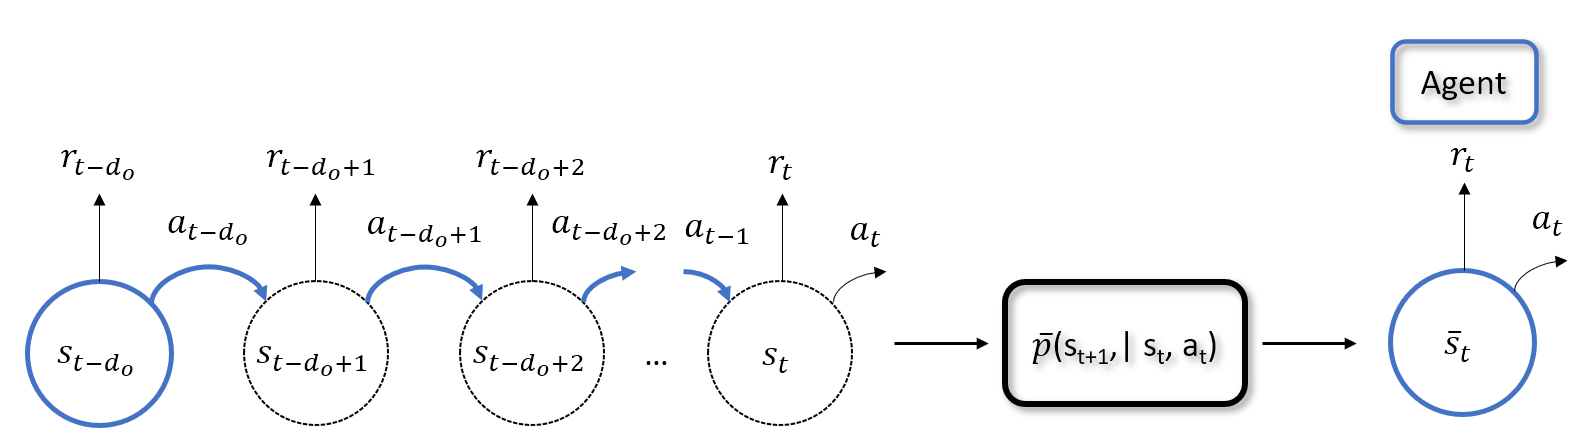
\includegraphics[width=15cm, keepaspectratio]{images/dmdp/modelbased_i_t.png}
                    \caption{Extended State $i_{t}$ is used as source of information to produce a representation $\bar{s}_t$ of the current unobserved state $s_t$, which is considered by the Agent as the current state.}
                    \label{fig:modelbased_i_t}
                \end{figure}
                
                Consider a CDMDP $\langle \mathbf{S}, \mathbf{A}, p, \mathbf{R}, d_o\rangle$. In general, at a certain time-step $t$ the Agent finds itself in an unknown state $s_t$, having available the knowledge contained in the extended state $i_t = \left( s_{t-d_{o}}, a_{t-d_{o}}, ..., a_{t-1}\right)$ and having learnt from some past trajectories an approximation $\bar{p}$ of the state-transition probability function $p$. The term \textit{extended state} is used as a synonym of the term \textit{augmented state}, outside the context of the Augmented approach. The information contained in the extended state $i_t$ is then used to infer the current state $\bar{s}_t$ (or a representation of the current state, such as a probability distribution over all possible current states) through the approximation $\bar{p}$. The specific details of the process of computing $\bar{s}_t$ and $\bar{p}$ are the subject of the specific implementation of a Model-Based algorithm, but it is important to notice that $\bar{s}_t$ may not be an element of the State Space $\mathbf{S}$. Infact, it will be referred to only as state \textit{representation}, in light of the fact that in more complex situation, such as stochastic environments or stochastic delays, it is impossible to predict an exact state. Thus Model-Based algorithm may instead rely on different concepts such as a Belief distribution over all the possible current states. Once the current state representation $\bar{s}_t$ is available, the Agent is able to select an action $a_t$ based on $\bar{s}_t$ (i.e. $a_t = \pi\left(\bar{s}\right)$) and to execute it. The Agent then finds itself in a new unknown state $s_{t+1}$, it perceives the observation of the old state $s_{t-d_{o}+1}$ and reward $r_t$ and the extended state $i_{t+1} = \left( s_{t-d_{o}+1}, a_{t-d_{o}+1}, ..., a_{t}\right)$ is available to the Agent. Figure \ref{fig:modelbased_i_t} shows the relationship between the extended state $i_t$ and the representation of the current state $\bar{s}_t$.
                \\\\
                As shown in Figure \ref{fig:modelbased_i_t}, Model-Based approach requires the decision making process to be split in two different steps:
                \begin{enumerate}
                    \item\textbf{State Representation:} at first, the knowledge available to the Agent is used to produce representation $\bar{s}_t$ of the current unobserved state $s_t$, possibly with a delay-independent size; 
                    \item\textbf{Action Selection:} then the "usual" action selection and decision-making process is carried out upon the result of the first step, selecting an action $a_t = \pi(\bar{s}_t)$ and executing it.
                \end{enumerate}
                This distinction is very important to describe this approach, because it allows for highlighting the main differences and similarities between Augmented and Memoryless approaches. As in the Augmented approach, Model-Based approach aims to use all the available information at each given time-step $t$: the extended state contains the same information contained in the augmented state. However, this information is not used as-is for learning a Policy function or a Value function, instead a current state representation $\bar{s}_t$ is produced. This first step is tackling directly the presence of delays by predicting, possibly meaningful, information about the current state $s_t$. This information is then the input for the second step, which is the usual decision-making with the fundamental difference of being carried out on some representation of $s_t$, possibly not even an actual state of the State Space. As in the Memoryless approach, the decision-making process is void of information about the delay, which is only implicitly expressed in $\bar{s}_t$, at the cost of learning how to produce a meaningful $\bar{s}_t$ from the available knowledge at each time-step $t$.
                \\\\
                The term \textit{Model-Based} stems from the peculiarities of the State Representation step: in order to produce the current state representation $\bar{s}_t$, the algorithm is forced to learn the dynamics of the environment is some way, thus basing its decisions on a model of the environment. This is in contrast to \textit{Model-Free} algorithm, where the knowledge of the dynamics of the environment are only implicitly learnt through the set of trajectories that are exploited to find the optimal policy.
                \\\\
                At last, it is important to highlight that developing a new Model-Based algorithm means developing a new method in order to carry out the State Representation step. Once the State Representation process is defined and working, the Action Selection step can be carried out by any of the state-of-the-art algorithm that already have been presented in the past. Infact, the studies presented in this section are focused on designing a new and more efficient way to produce the state representation, rather than the action selection process. In the same way, the focus of this research work is to define a new structured network (which will be referred to as \textit{module} in Chapter \ref{chp:ow}), that is able to produce a state representation in different environmental settings. In this research, the Action Selection step is handled by an already defined and presented state-of-the-art algorithm (Section \ref{sota:trpo}).
                
                
            \subsubsection{Model-Based Simulation (MBS)}
                \begin{algorithm}[t]
                    \SetAlgoLined
                    \KwData{CDMDP $M = \langle \mathbf{S}, \mathbf{A}, p, \mathbf{R}, d_o\rangle$; \newline Augmented State $i_t = \left( s_{t-d_{o}}, a_{t-d_{o}}, a_{t-d_{o}+1}, ...,  a_{t-1}\right)$.}
                    \KwResult{Optimal Action for current (unobserved) State: $\pi^{*}(\bar{s}_t)$}
                    Construct a regular undelayed MDP $\bar{M} = \langle \mathbf{S}, \mathbf{A}, \bar{p}, \mathbf{R}\rangle$ where $\bar{p}(s' | s, a) = 1$ for each triple $(s, a, s')$ in which the state $s'$ is the most likely state visited as a consequence of executing action $a$ in state $s$ in deterministic Environments or the correspondent expected state in mildly stochastic Environments, in the original CDMDP\;
                    Find the optimal Value function $\bar{v}_{*}$ and the optimal Policy function $\bar{\pi}_{*}$ for $\bar{M}$\;
                    Compute the current unobserved state $\bar{s}_t$ by applying the action sequence contained in the augmented state $i_t$ $\left(a_{t-d_{o}}, a_{t-d_{o}+1}, ...,  a_{t-1} \right)$ starting from $s_{t-d_{o}}$ according to $\bar{p}$\;
                    Compute the optimal action to be executed in $\bar{s}_t$ according to $\bar{\pi}_{*}$: $\pi^{*}(\bar{s}_t)$, which is interpreted by the Agent as $\pi^{*}(\bar{s}_t)$.
                    \caption{Model-Based Simulation}
                    \label{algo:mbs}
                \end{algorithm}
                A significant contribution to this approach is given by \pcite{delay:mbs}, which presents Model-Based Simulation (MBS), a planning algorithm that exploits all the relevant concepts along with important theoretical results. \newline
                Given a CDMDP $\langle \mathbf{S}, \mathbf{A}, p, \mathbf{R}, d_o\rangle$, Model-Based Simulation idea is that the information available to the Agent at a given time-step $t$, which is usually summarized in the extended state $i_t = \left( s_{t-d_{o}}, a_{t-d_{o}},..., a_{t-1}\right)$, can be exploited to retrieve an approximation of the current unknown state $s_t$, which will be denoted by $\bar{s}_t$. In order to compute $\bar{s}_t$, MBS constructs a standard MDP $\langle \mathbf{S}, \mathbf{A}, \bar{p}, \mathbf{R}\rangle$, where $\bar{p}$ is an approximation of the original state-transition function $p$ and it is defined in the following way:
                \[  \bar{p}(s_t, a_t, s_{t+1}) = 1 \] 
                
                \begin{itemize}
                    \item if $s_{t+1}$ is the most likely outcome of executing $a_t$ in $s_t$ in case of a discrete State Space $\mathbf{S}$, or
                    \item if $s_{t+1}$ is the expected outcome in case of a continuous State Space $\mathbf{S}$.
                \end{itemize}
                
                Once $\bar{p}$ is available, the Agent can recursively apply it to the extended state $i_t = \left( s_{t-d_{o}}, a_{t-d_{o}},..., a_{t-1}\right)$ in order to compute the sequence of approximated states $(\bar{s}_{t-d_{o}+1}, \bar{s}_{t-d_{o}+2}, ..., \bar{s}_{t-1}, \bar{s}_{t})$. Finally, the Agent is able to select the next action by assuming that the current state is $\bar{s}_{t}$. The complete algorithm is detailed in Algorithm \ref{algo:mbs}.
                \\\\
                In order to relate to the terminology used in the section \ref{subsubs:mbapproach:general}, the approximation of the current state $\bar{s}_t$ can be considered as a pratical example and implementation of state representation, while $\bar{p}$ is exactly the approximation of the state-transition function $p$. Thus, in the case of Model-Based Simulation, the process that computes the state representation of the current unknown state $s_t$ directly involves an approximation of the state-transition $\bar{p}$ function and it outputs an element of the State Space $\mathbf{S}$.
                \\\\
                Another important contribution given by \pcite{delay:mbs} is the theoretical study about the consequences of the presented approximation. Introducing an approximation also implies introducing a certain amount of error within the discussed algorithm. In practice, the Agent will always act "as if" the current unknown state $s_t$ is exactly its state representation $\bar{s}_{t}$, which is false in general. As a consequence, the optimal action selection cannot be carried out precisely, which in turn results in a loss of performances w.r.t. the undelayed process. However, it is proven that the loss of performances is bounded in case the underlying undelayed dynamics of the environment has the following properties:
                
                \begin{itemize}
                    \item Deterministic and Finite: the undelayed MDP $\langle \mathbf{S}, \mathbf{A}, p, \mathbf{R}\rangle$ is such that $|\mathbf{S}| < \infty$ and $\forall s \in \mathbf{S} \; \exists s' \in \mathbf{S}: \; p(s,a,s') = 1$;
                    \item Deterministic and Continuous: the undelayed MDP $\langle \mathbf{S}, \mathbf{A}, p, \mathbf{R}\rangle$ is such that $\mathbf{S}$ and $\mathbf{A}$ are continuous and $\forall s \in \mathbf{S} \; \exists s' \in \mathbf{S}: \; p(s,a,s') = 1$;
                    \item Mildly Stochastic and Finite: the undelayed MDP $\langle \mathbf{S}, \mathbf{A}, p, \mathbf{R}\rangle$ is such that $|\mathbf{S}| \leq \infty$ and $\exists \delta \leq 0$ such that $\forall s \in \mathbf{S} \; \exists s' \in \mathbf{S}: \; p(s,a,s') \geq 1 - \delta$.
                \end{itemize}
                
                This result is very important because it avoids arbitrarily worse performances w.r.t. the undelayed counterpart, which would greatly impact the applicability of the approach.
            
            \subsubsection{A Recurrent Network Algorithm}
                \label{subsub:modelbased_recurrent}            
                \pcite{delay:ssbm} present a Model-Based algorithm in order to cope with the presence of execution delay, using as environment a famous competitive videogame in which the notion of delay is identified as the reaction time an average player is able to express. The approach taken in this study is inspired by the experimental psychology explanation of how the human brain tackles its continuous interaction with physical environments: constantly predicting the immediate future, so that the body is able to react in time regardless of the natural latency that movements require. \newline
                The proposed algorithm makes use of a Recurrent network based on Gated Recurrent Unit (\pcite{dl:gru}) in order to iteratively predict the sequence of unknown states that are not yet known to the Agent. Given a CDMDP $\langle \mathbf{S}, \mathbf{A}, p, \mathbf{R}, d_a\rangle$, at each time-step $t$ the knowledge contained in the extended state $i_t = \left( s_{t}, a_{t-d_a},..., a_{t-1}\right)$ is available to the Agent. The currently known state $s_t$, denoted from now on as $s_{t, 0}$, is used as input to a GRU along with the core hidden state $h_t$, denoted from now on as $h_{t, 0}$ which is the result of the last iteration of the recurrent network, in order to produce the next core hidden state $h_{t, 1}$ and the core output $o_{t, 0}$. At this point, the triple $(s_{t, 0}, a_{t-d_a}, o_{t, 0})$ is used as input to a learnt state-transition function $\bar{p}$ in order to produce the prediction for the next state, $s_{t, 1}$:
                \[ s_{t, 1} = \bar{p}(s_{t, 0}, a_{t-d_a}, o_{t, 0}) \]
                Once $s_{t, 1}$ is available, it can be used along with $h_{t, 1}$ as input to a GRU in order to produce the next core hidden state $h_{t, 2}$ and the next core output $o_{t, 2}$. The new triple $(s_{t, 1}, a_{t-d_a+1}, o_{t, 1})$ is used to produce $s_{t, 2}$ thorugh $\bar{p}$ and the iteration is repeated. Each step $i$ can be summarized as follows:
                
                \begin{align*}
                    h_{t, i+1}, o_{t, i} &= GRU(s_{t, i}, h_{t, i})\\
                    s_{t, i+1} &= \bar{p}(s_{t, 1}, a_{t-d_a+1}, o_{t, 1})
                \end{align*}
                
                This iterative process is carried out $p$ times, with $p \leq d_a$ being an hyperparameter of the model. In the last iteration, the core $o_{t, p}$ is produced and used as input to the policy $\pi$ in order to select action $a_t$. As usual, the effect of action $a_{t-d_a+1}$ is observed and the Agent will find itself in the extended state $i_t = \left( s_{t+1}, a_{t-d_a+1},..., a_{t}\right)$. Figure \ref{fig:modelbased_ssbm} provides a visualization of the iterative process that produces the core outputs.
                \\\\
                As it can be observed, the state representation proposed by \pcite{delay:ssbm} is the core output $o_{t,p}$, which is not an element of the State Space $\mathbf{S}$, but rather a vector built by the p-th Gated Recurrent Unit. The idea behind the choice of not using a predicted element of the state space, which is also already available as $s_{t,p}$ in this algorithm, is that it is possible to compress useful information about the current state (or current state distribution, in case of stochasticity involved) in a finite vector used as input to the policy $\pi$. In this way, the input space of the policy function is not the State Space $\mathbf{S}$. \newline
                It is important to highlight this concept because it is closely related to the scope of this research, which also tries to compress information about the current state distribution in a finite vector, as it is presented in Chapter \ref{chp:ow}. 
                \\\\
                In order for the core output $o_{t,p}$ to represent useful information, the whole network describe needs to be trained accordingly. Infact, the predictive model constituted by GRUs and the learnt state-transition probability function $\bar{p}$ is trained against the actual dynamics of the environment: the sequence of predicted states $(s_{t, 1}, s_{t, 2}, ..., s_{t, p})$ is compared to the actually experienced sequence of state $(s_{t+1}, s_{t+2}, ..., s_{t+p}$ in a Regression fashion. In this way, the core hidden state $h$ and core output $o$ are driven towards compressing useful information about the current unknown state $s_{t+d_a}$ in which the Agent will execute the chosen action $a_t$. In this regards, experiments have highlighted how the best choice of the hyperparameter $p$ is exactly the execution delay $d_a$. This is also intuitively reasonable: in the case in which $p = d_a$, at each time-step, the Agent is trained on the entire sequence of states that separates it from the state in which it will execute action $a_t$, thus resulting in a more accurate prediction $s_{t, p}$, which in turn is translated in a more meaningful core output $o_{t, p}$. The other two possible cases are: $p < d_a$, the Agent never learns to predict the current state $s_t$ and its estimates refers to an earlier, different, state $s_{t,p}$; $p > d_a$, the Agent learns to predict more states than necessary, making the overall network more complex and the $s_{t, d_a}$ prediction less accurate. These conclusions are also confirmed by the results of this research (Chapter \ref{chp:results}).
                
                \begin{figure}
                    \centering
                    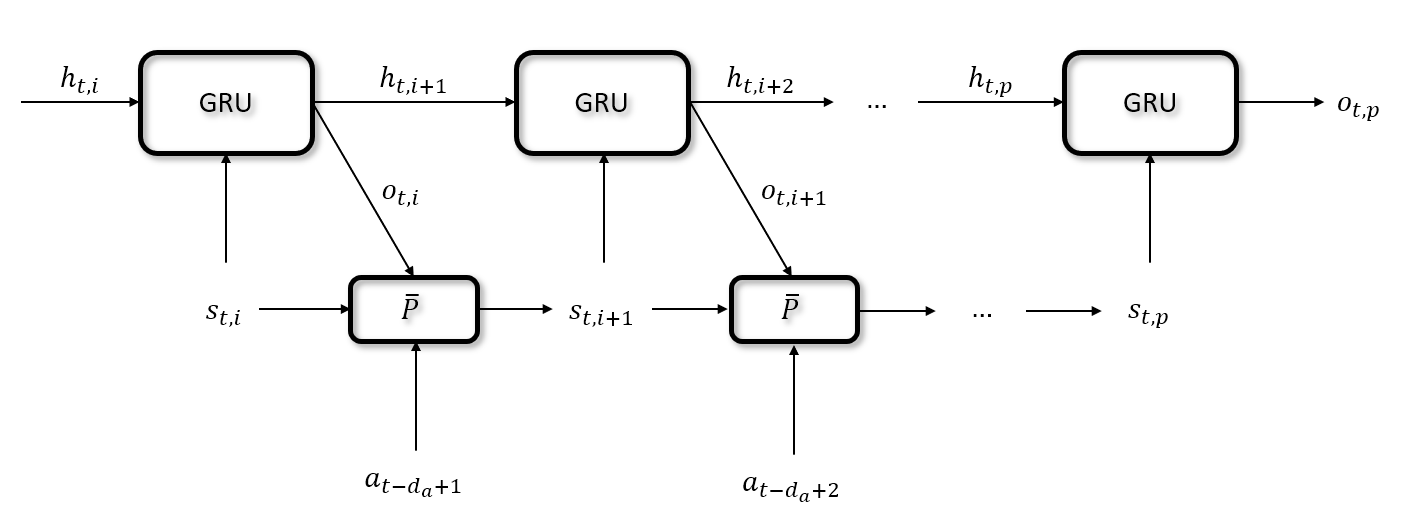
\includegraphics[width=15cm, keepaspectratio]{images/dmdp/modelbased_ssbm.png}
                    \caption{The iterative process of predicting the sequence of states $s_{t, i}$ that will occur in the next $p$ steps along with producing the correspondent core outputs $o_{t, i}$.}
                    \label{fig:modelbased_ssbm}
                \end{figure}
                
            \subsubsection{Model-Based Approach for Stochastic Delays} 
                \begin{figure}[t]
                    \centering
                    
                    \begin{subfigure}[b]{.45\textwidth}
                        \centering
                        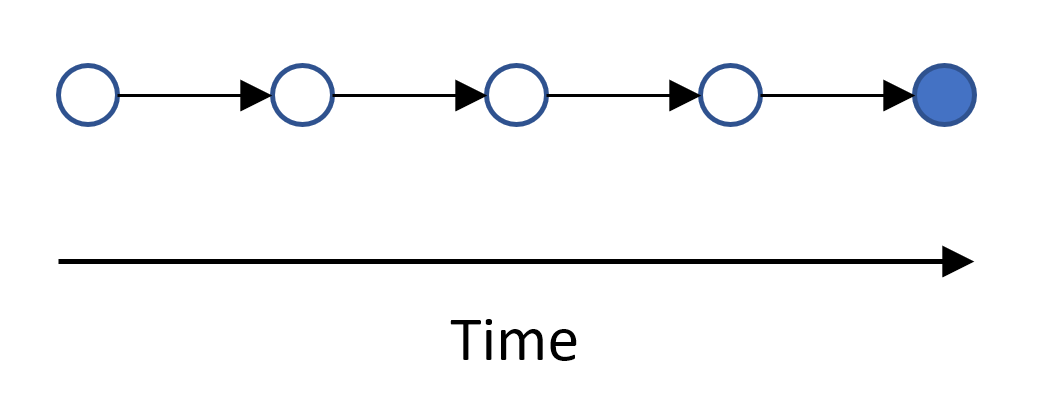
\includegraphics[width=\textwidth]{images/dmdp/modelbased_stochastic_1.png}
                        \caption{Deterministic delay in a deterministic environment.}
                        \label{fig:modelbased_stochastic_1}
                    \end{subfigure}
                    \hfill
                    \begin{subfigure}[b]{.45\textwidth}
                        \centering
                        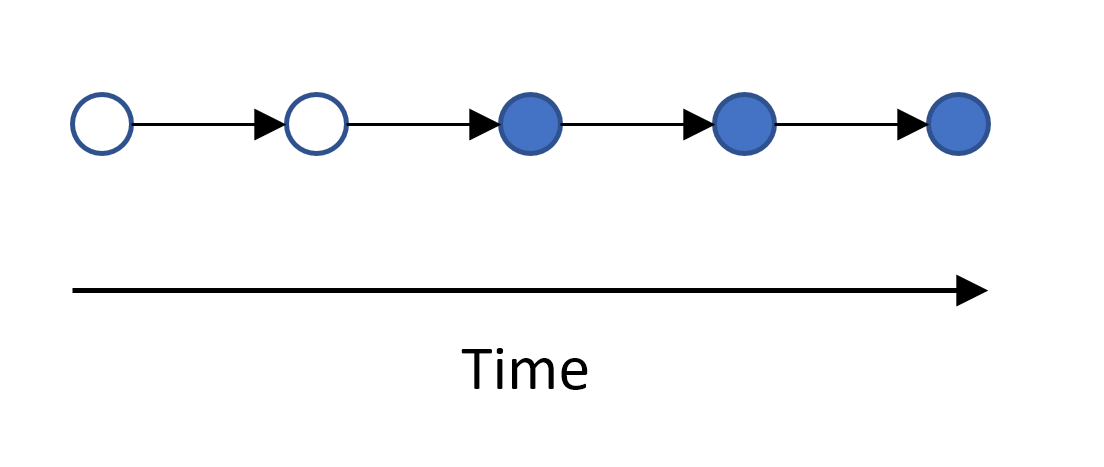
\includegraphics[width=\textwidth]{images/dmdp/modelbased_stochastic_2.png}
                        \caption{Stochastic delay in a deterministic environment.}
                        \label{fig:modelbased_stochastic_2}
                    \end{subfigure}
                    
                    \begin{subfigure}[b]{.45\textwidth}
                        \centering
                        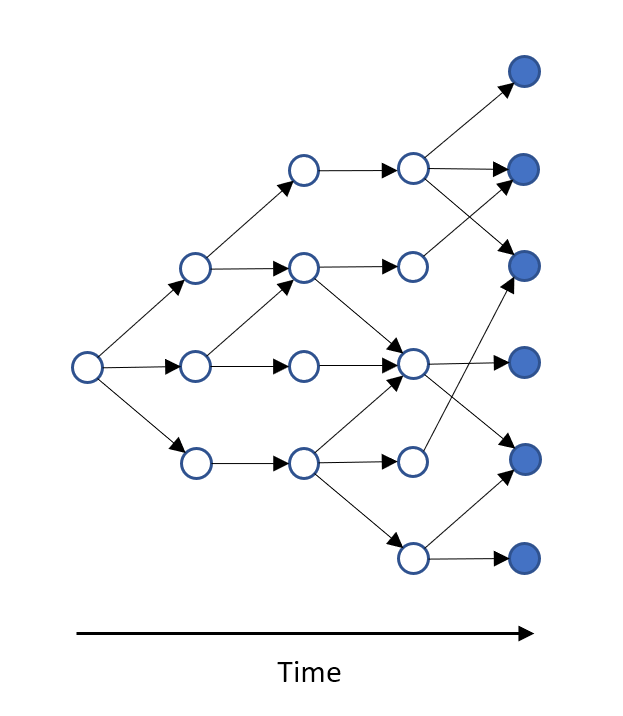
\includegraphics[width=\textwidth]{images/dmdp/modelbased_stochastic_3.png}
                        \caption{Deterministic delay in a stochastic environment.}
                        \label{fig:modelbased_stochastic_3}
                    \end{subfigure}
                    \hfill
                    \begin{subfigure}[b]{.45\textwidth}
                        \centering
                        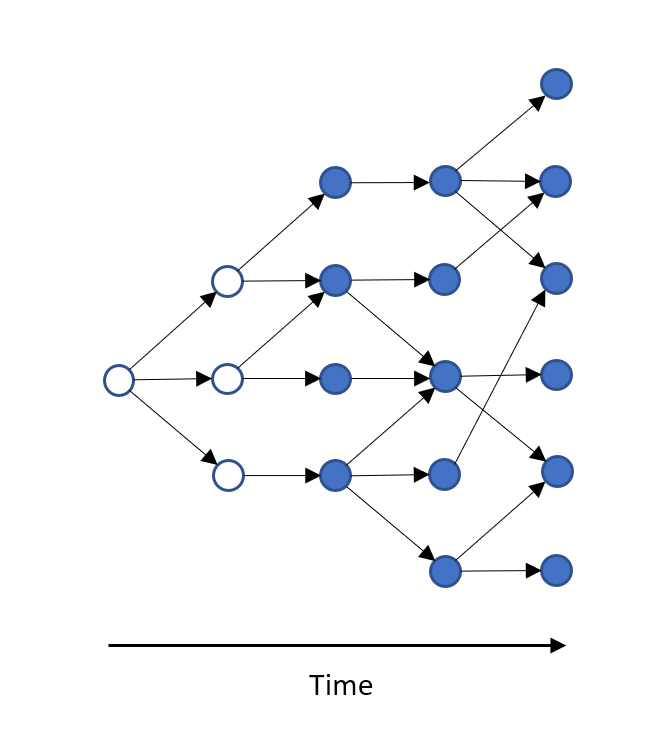
\includegraphics[width=\textwidth]{images/dmdp/modelbased_stochastic_4.png}
                        \caption{Stochastic delay in a stochastic environment.}
                        \label{fig:modelbased_stochastic_4}
                    \end{subfigure}
                    
                    \caption{An example of how stochasticity impact the current unknown state distribution. In each figure, each circle represents a state and each arrows an action. The Agent last known state is the left-most state. The other white states are states that could have been reached by the Agent, while the blue states are states in which the Agent could be now. Both white states and blue states are unknown because the presence of delays.}
                    \label{fig:modelbased_stochastic}
                \end{figure}
            
                Throughout the previous paragraphs delays is assumed constant so to focus on other relevant aspects of the approach. Nevertheless, important observations can be made for the case of stochastic delays. Given the definition of Model-Based approach presented in Section \ref{subsubs:mbapproach:general}, the impact of stochasticity in the delay process $d_o(t)$ affects only the State Representation step, since the extended state $i_t$ will contain a variable number of actions depending on the sampled delay at time-step $t$. The fact that $i_t$ has a variable number of actions actually has a huge impact from different point of views, especially in the design of the algorithm. \newline
                The structured component that implements the State Representation step needs to be able to cope with a variable length input in some way. From the basic computational point of view, the network needs to be able to accept inputs of different lengths at each step, which is not a trivial task: for example, standard neural networks are not able to manage such inputs, while recurrent networks such as GRU or Long-Short Term Memory (LSTM, \pcite{dl:lstm}) are capable of handling them, but with a computational cost that increase in the length of the input. From the learning difficulty point of view, the context of stochastic delays is much more complex: the model needs to be able to output relevant state representations not only for fixed amount of steps in the future, but for different amounts, at once. \newline
                The State Representation $\bar{s}_t$ is directly used as input for the Action Selection step. In the case of stochastic delays, it is not trivial to design the size of $\bar{s}_t$: if the structured network that computes it  mantains its variable length, then the variable length issue is propagated to the Action Selection step, thus to the policy function. On the other hand, having a fixed length $\bar{s}_t$ means that information about the current state distribution is compressed on a fixed length vector, which still needs to be able to contain a relevant amount of information so that the Action Selection step can achieve good performances overall. \newline
                At last, Figure \ref{fig:modelbased_stochastic} shows the differences between the deterministic delay and the stochastic delay cases, along with deterministic and stochastic environment. Intuitively, the case of deterministic delays in a deterministic environment is the easiest to solve and, theoretically speaking, knowing the dynamics of the environment perfectly leads to solving the State Representation step in a closed form: applying each action recursively to the last known state would always generate the exact sequence of states that will be perceived by the agent in the future. In practice, there is no other state in which the Agent could be. The presence of stochasticity can greatly complicate this setting, since the currently unknown state could greatly vary both in the Stace Space $\mathbf{S}$ and in the time-step $t$, leading to a more elaborated probability distribution and, in turn, to a much more complex state-transition probability function which needs to be learnt by the Agent. 
                
            \subsubsection{Advantages and Disadvantages}
                Advantages and disadvantages of the Model-Based approach stem from the comparison against the other two approaches presented so far. Infact, as said in the introduction, the Model-Based approach represents a middle ground between the Augmented and Memoryless approach, focusing on escaping the inherent complexity of the first while incorporating more knowledge of the delay w.r.t. the second. 
                \\\\
                As stated in Theorem \ref{th:dmdpobscomplexity}, the Augmented approach heavily suffers from the computational complexity point of view: incorporating the knowledge of the delay directly within the state of the new, augmented MDP to be learnt has the side effect of making it solvable in exponential time w.r.t. the amount of delay, as proven by \pcite{delay:mbs}. Instead, the Model-Based approach is able to incorporate knowledge about delays escaping the exponential time complexity: the Agent learns upon a representation of the current state $\bar{s}_t$, which can be designed to be of fixed size regardless of the amount of delay present. Thus, this class of algorithms is able to solve the original DMDP in polynomial time, as demonstrated by \pcite{delay:mbs}. As usual, this advantage does not come for free: the Model-Based approach needs to learn the dynamics of the underlying DMDP and the higher the amount of delay, the more difficult is the task, as shown in Figure \ref{fig:modelbased_stochastic}. From an intuitive point of view, the Augmented approach can be seen as a Model-Based approach in which the representation $\bar{s}_t$ of the current state $s_t$ is the extended state $i_t$, thus the State Representation step highlighted in Section \textit{General Approach} is the identity function. Figure \ref{fig:modelbased_appr_augmented} shows this concept from a visual perspective. 
                \\\\
                At the same time, Model-Based approach cannot be as fast as Memoryless approach in general, exactly because of its need of learning the dynamics of the underlying MDP. In fact, Memoryless Approach is almost completely neglecting knowledge about delays, leaning towards solutions that may be not even converge to the optimal solution, as \pcite{delay:memoryless} observes, but can be found by using traditional algorithms with little or any modifications. As the result of this research will show, also Model-Based algorithms suffer from optimizing towards suboptimal solutions, but the underlying hypothesis is that they offer a better trade-off between computational complexity and integrating knowledge about delays, thus leading to better solutions. From an intuitive point of view, Memoryless Approach can be seen as a Model-Based approach in which the State Representation $\bar{s}_t$ of the current state $s_t$ is the first component of the extended state, $s_{t-d_o}$. Thus, any State Representation $\bar{s}_t$ that requires more complex computation will result in a more complex approach. Figure \ref{fig:modelbased_appr_memoryless} shows this concept from a visual perspective.
                \\\\
                Aside from the computational complexity analysis, Model-Based approach offers a wider range of possibilities, with Augmented and Memoryless approaches at its extremes. For this reason, Model-Based approach aims to provide a better trade-off between the completeness of the Augmented approach and the lightness of the Memoryless approach, hopefully towards better performances overall. As explained in previous sections, designing a Model-Based algorithm requires important decision-making towards the State Representation step, specifically about which kind of networks are suitable for the scope of the algorithm and thus which are the delay and environment properties that can be handled by the algorithm. In other words, the State Representation step answers to the question of how can the information available to the Agent be used efficiently in order to produce a meaningful information vector that is then used as input for the Action Selection step. This approach allows for improving or changing the State Representation step without affecting the Action Selection step, which can be carried out by past, current or even future state-of-the-art algorithms. Thus, another important advantage of the Model-Based approach is the wide applicability with existent or future RL algorithms.
                
                \begin{figure}
                    \centering
                    
                    \vspace{1.0cm}
                    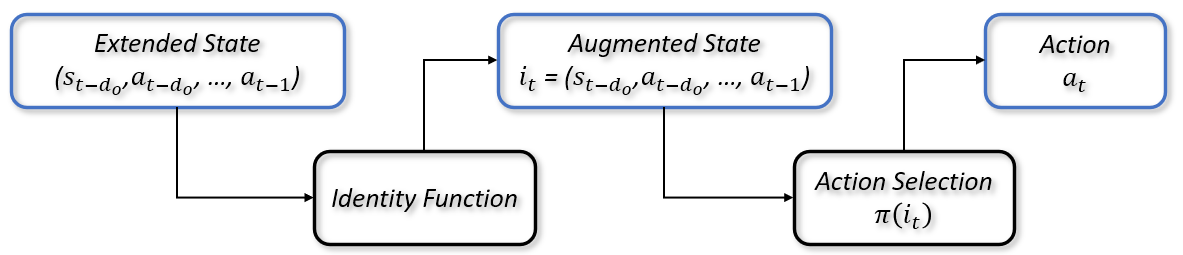
\includegraphics[width=15cm, keepaspectratio]{images/dmdp/modelbased_appr_augmented_2.png}
                    \caption{Augmented Approach presented as a particular case of Model-Based Approach. Knowledge available or inferred by the Agent is highlighted in light blue and computational steps are highlighted in black. State Representation's black box is an identity function, while Action Selection is the usual decision-making choice.}
                    \label{fig:modelbased_appr_augmented}
                    
                    \vspace{2.5cm}
                    
                    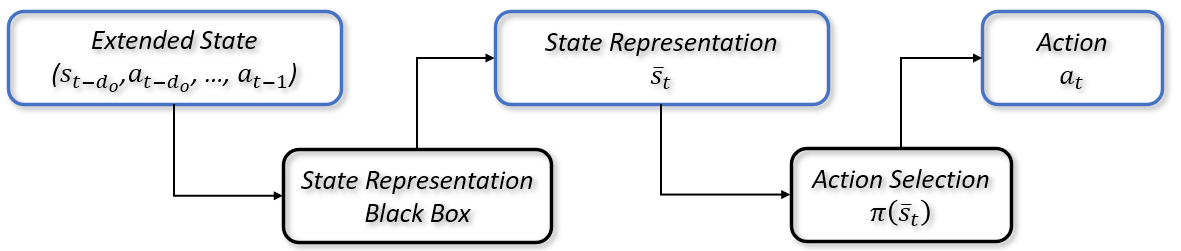
\includegraphics[width=15cm, keepaspectratio]{images/dmdp/modelbased_appr_modelbased_2.png}
                    \caption{Model-Based Approach presented as sequence of steps, knowledge available or inferred by the Agent is highlighted in light blue, while computational steps are highlighted in black. State Representation is described as a black box, while Action Selection is the usual decision-making choice.}
                    \label{fig:modelbased_appr_modelbased}
                    
                    \vspace{2.5cm}
                    
                    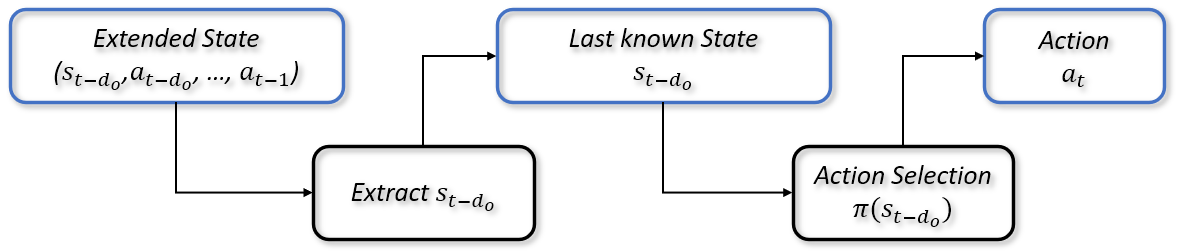
\includegraphics[width=15cm, keepaspectratio]{images/dmdp/modelbased_appr_memoryless_2.png}
                    \caption{Memoryless Approach presented as a particular case of Model-Based Approach. Knowledge available or inferred by the Agent is highlighted in light blue and computational steps are highlighted in black. State Representation's black box only extracts the last known observation from the extended state, while Action Selection is the usual decision-making choice.}
                    \label{fig:modelbased_appr_memoryless}
                    \vspace{1.0cm}
                \end{figure}
        
    \newpage
    \section{Partially Observable MDP}
        \label{sota:pomdp}
        % Section Schema
        % Introduction on POMDP citing Chapter 2 Section on Belief
        %   - Subsection: Link between DMDP and POMDP (extendedstate as observation)
        %   - Subsection: PSD
        %   - Subsection: RPSP
        %   - Subsection: Link between RPSP and Model-Based Approach + Advantages
        
        This section is dedicated to present the similarities between the Delay MDP framework and the Partially Observable MDP framework. Establishing a link between the two frameworks allows for also establishing a connection between the correspondent literatures. Since DMDP research is far less explored than POMDP research, this process is especially beneficial for first: approaches, theorems and concepts established for POMDP framework can be translated into the DMDP framework and they may be useful as a starting point to advance research and develop new solutions. Infact, two specific studies in POMDP research are presented as they have been important in the process of developing this research original work: Section \ref{subs:psd} is focused on Predictive-State Decoder (PSR) architecture, which introduces the idea of evaluating the network using a second performance measure to drive the internal state of the network towards a meaningful quantity; while Section \ref{subs:rpsp} presents Recurrent Predictive-State Policy networks, an direct application of the PSR paradigm.
        
        \subsection{Connection between DMDP and POMDP}
            In Section \ref{subs:pomdp}, the concepts of Observation function and Belief have been presented and they can be expanded further now, after having presented the different DMDP approaches in Section \ref{sota:delay_approaches}. The core issue of POMDP framework is that, at each time-step $t$, the Agent perceives an observation $o_t$ of the current state $s_t$ and the relationship between observations and states is not one-to-one: observing $o_t$ may be resulting from several states $s_t$. Thus the Agent needs to plan its actions not only according to the dynamics of the environment, but also understanding them through incomplete observations. The concept of observation is generic in the literature, since it may represent any information that the Agent is able to perceive from the current state of the environment.
            \\\\
            While the terminology is different, the class of DMDP Agents is actually working under the same assumption of POMDP Agents: at each time-step $t$, the Agent perceives the information contained in the extended state $i_t = (s_{t-d_o}, a_{t-d_o}, ..., a_{t-1})$ which may be correspondent to several currently unknown states $s_t$, more specifically the set of states that are reachable from $s_{t-d_o}$ by executing the sequence of actions $(a_{t-d_o}, ..., a_{t-1})$. The differences lie in how the Agent makes use of the extended state $i_t$, i.e. which information is extracted and reasoned upon, thus in which approach is taken by the agent.
            
            \subsubsection{Augmented Approach as POMDP}
                As presented in Section \ref{subs:augmentedapproach}, the Augmented approach makes direct use of the entire extended state $i_t$ at each time-step $t$. In this sense, when translated in the POMDP framework, the entire extended state is the Agent's observation at each time-step: $o_t = i_t$. In this way, it is also possible to specifically define the Observation function $O$ for the Augmented approach:
                
                \[ O(s_t|o_t) = O(s_t|i_t) = \sum_{i = t - d_o}^{t-1} p(s_{i+1}|s_{i}, a_{i}) \]
                
                where $p$ is the state-transition probability function of the environment. Thus it is possible to construct a Belief of the current unknown state $s_t$ and act accordingly.
            
            \subsubsection{Memoryless Approach as POMDP}
                Memoryless approach does not fully utilize the extended state $i_t$, as explained in Section \ref{subs:memorylessapproach}. Regardless of the fact that other mechanism in the algorithm may be able to use information about the presence of delay, the Agent's observation is the last known state: $o_t = s_{t-d_o}$. As in the previous section, it is possible to specifically define the Observation function $O$ for the Memoryless approach:
                
                \[ O(s_t|o_t) = O(s_t|s_{t-d_o}) = \sum_{i = t - d_o}^{t-1} \sum_{a \in \mathbf{A}} p(s_{i+1}|s_{i}, a)\]
                
                where $p$ is the state-transition probability function of the environment. As in the previous section, it is possible to define a Belief of the current unknown state $s_t$. \newline
                Furthermore, it is possible to observe that Memoryless approach is actually a solution directly borrowed from the POMDP literature, where Memoryless algorithms are algorithms that makes only use of the last known observation $o_t$ in order to plan the next action. In the same way, Memoryless policy makes only used of the last known state $s_{t-d_o}$ in order to plan the next action.
            
            \subsubsection{Model-Based Approach as POMDP}
                Model-Based approach can not be immediately represented as POMDP, since the process of extracting information from the extended state $i_t$ is not trivial and thus implies several design choices which alter the final result. As explained in Section \ref{subs:modelbasedapproach}, the Agent's decision-making process is split into two different steps: the result of the first step, the State Representation step, is the observation $o_t$, which is then used by the Action Selection step to effectively select the next action $a_t$. \newline
                Thus, it is of interest for Model-Based approach research to look into the POMDP research for new solutions and concepts that may help to develop new and more efficient algorithms and for this reason the next sections are focused on presenting results from the POMDP literature that have been helpful towards the development of this research's original work.
        
        \newpage
        \subsection{Predictive-State Decoders}
            \label{subs:psd}
            \pcite{pomdp:psd} expands on the existing solution of using Recurrent Neural Networks (RNN) for dealing with POMDP framework, presenting a new architecture called Predictive-State Decoder, which is specifically designed to cope with the main issues of the Recurrent models. 
            
            \subsubsection{Recurrent Models}
                
                \begin{figure}[t]
                    \centering
                    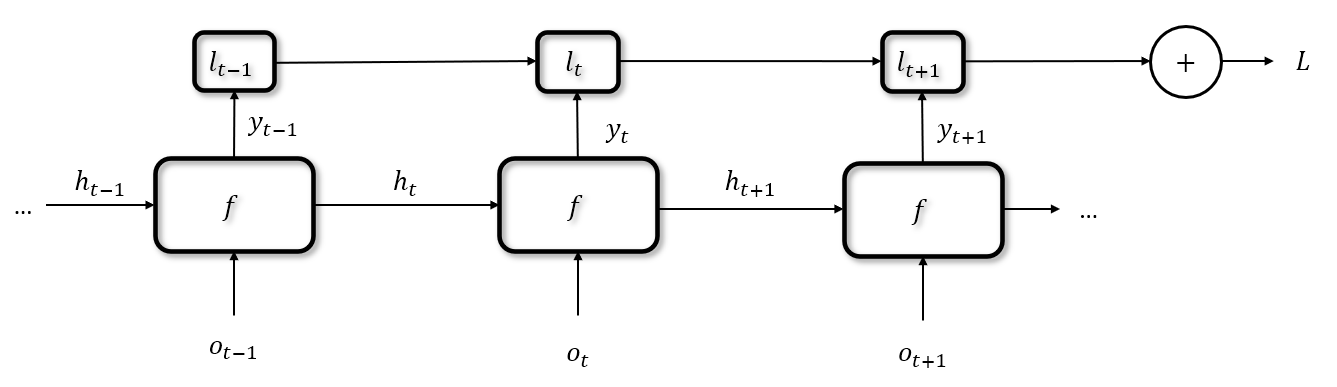
\includegraphics[width=15cm, keepaspectratio]{images/pomdp/pomdp_rnn.png}
                    \caption{Recurrent model. At each time-step $t$, the model $f$ receives as input the previous internal state $h_{t-1}$ and the latest observation $o_{t-1}$ in order compute the next internal state $h_{t}$ and the prediction $y_{t}$. The prediction $y_t$ is then used to compute the current loss $l_t$. All losses $l_t$ are summed together to retrieve Loss function $L$.}
                    \label{fig:pomdp_rnn}
                \end{figure}
                
                Recurrent Neural Networks have been proposed as a solution to Partially Observable MDP due to their ability of maintaining and updating an internal state, denoted $h_t$, at each time-step $t$. In general, the main objective of Recurrent models is to find a model $f$ that receives as input the last observation $o_t$ and it is able to recursively update its internal state $h_t$ while predicting a target variable $y_t$. The sequence of target variables is then collected and used to compute the Loss Function $L$, through which the recurrent network is optimized:
                
                \[ \min_{f} L = \min_{f} \sum_{t} l(f(h_t, o_t)) \]
                
                \noindent
                This process is illustrated in Figure \ref{fig:pomdp_rnn}. In POMDP framework, Recurrent models have the objective of selecting the next action $y_t = a_t$ while updating the current internal states $h_t$ and the underlying assumption is that by optimizing the whole network towards the optimal performance w.r.t. the collected rewards, the internal state updates will eventually lead $h_t$ to a meaningful representation of the current unknown state. In practice, as \pcite{pomdp:psd} observe, the absence of a loss function directly specified over $h_t$ makes this task very difficult to achieve and a Recurrent model that does not encode meaningful information within its internal state is bound to perform poorly.
                
            \subsubsection{Predictive-State Decoders}
            
                \begin{figure}[t]
                    \centering
                    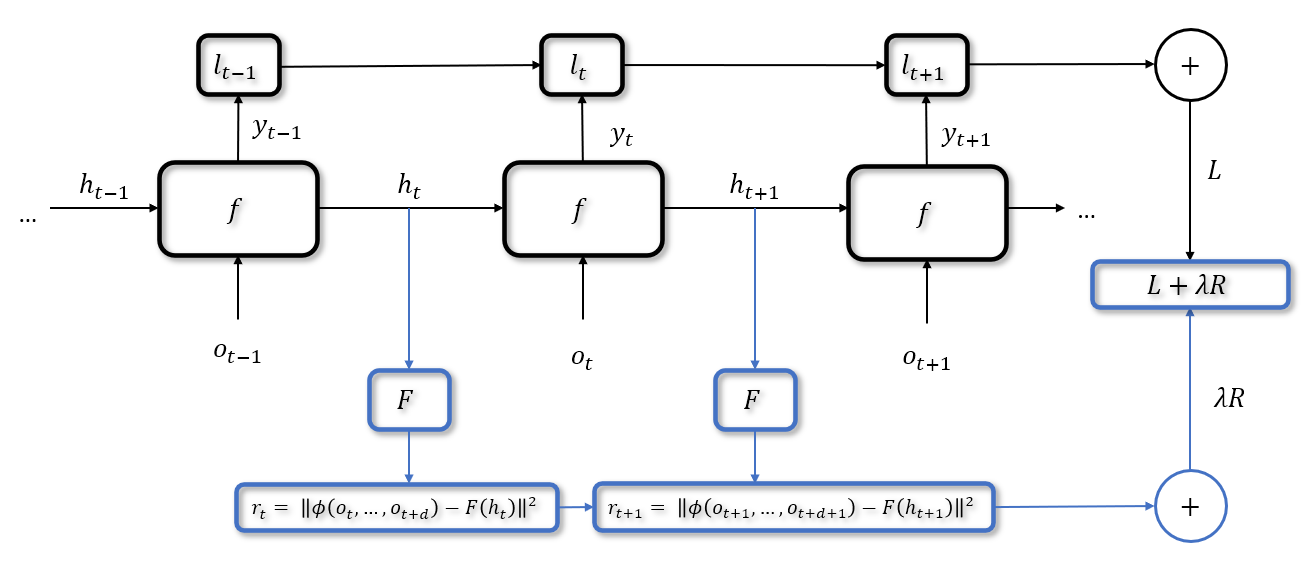
\includegraphics[width=15cm, keepaspectratio]{images/pomdp/pomdp_psd.png}
                    \caption{Predictive-State Decoder, the differences with the Recurrent model are highlighted in light blue. In addition to the Recurrent model, at each time-step $t$, the internal state $h_t$ is first encoded through $F$ and then used to compute the current Predictive-State loss $r_t$. All Predictive-State losses $r_t$ are summed together to retrieve the Predictive-State loss $R$, which is then weigthed by $\lambda$ and added to $L$.}
                    \label{fig:pomdp_psd}
                \end{figure}
            
                The solution proposed by \pcite{pomdp:psd} is to add a new portion to the recurrent architecture that is dedicated to evaluate the internal states during the training process. Its purpose is to assess how much the internal state is close to a meaningful target variable: the sequence of future observations $(o_{t+1}, o_{t+2}, ...)$. This evaluation is then added to the Loss function through which the entire architecture is optimized. This allows for finding an internal state $h_t$ only by means of quantities observed by the Agent during its interaction with the environments- The class of methods that allows for this behavious is called Predictive-State Representations (PSR). \newline
                In practice, at each time-step $t$, the L2-Norm between $h_t$ and the sequence of future observation $(o_{t+1}, o_{t+2}, ..., o_{t+d})$ is computed. In order to be able to compute the L2-Norm starting from arbitrary sizes of $h_t$, an encoder $F$ is added. The sequence of L2-Norm computed at each time-step $t$ is then collected to form a new loss Function, the Predictive-State loss function:
                
                \begin{definition}[Predictive-State Loss function $R$]
                    \[ R = \sum_{t=0}^{T} \| F(h_t) - \phi([o_{t+1}, o_{t+2}, ..., o_{t+d}])\|^{2}\]
                    
                    where $\phi$ denotes some feature functions chosen for the future observations.
                \end{definition}
                
                \noindent
                The Predictive-State loss function $R$ is then weigthed by a factor $\lambda$ and added to the previously defined loss function:
                
                \[ \mathbb{L} = L + \lambda R\]
                
                where $\lambda$ is used to tune the importance of $R$ within the entire loss function. This architecture is called Predictive-State Decoder (PSD) and it is shown in Figure \ref{fig:pomdp_psd}. 
            
            \subsubsection{Multi-Task Learning}
                Predictive-State Encoder architecture can be interpreted as an example of Multi-Task Learning (MTL, \pcite{ml:mtl}). Multi-Task Learning is a particular instance of Machine Learning methods that are able to learn upon different tasks at the same time, with the purpose of improving the overall performances of algorithm by letting the different tasks interact together. In the Predictive-State Decoder example, the Agent is both learning how to optimize the action selection process towards higher rewards and a meaningful internal state $h_t$. This two tasks are not completely independent, infact the underlying hypothesis is that driving $h_t$ towards the representation of meaningful information will lead to a better action selection. This type of Multi-Task Learning is important for the scope of this research, since its concepts provided guidance for part of the design or the original work.
        
        \newpage
        \subsection{Recurrent Predictive State Policy Networks}
        \label{subs:rpsp}
            A step forward in the research on Predictive-State Representations and Multi-Task Learning for POMDP is taken by \pcite{pomdp:rpsp}, who present a complete and structured network called Recurrent Predictive State Policy (RPSP). \newline
            RPSP network is divided into two main components with their distinct set of parameters that interact together: the first component is a Recurrent Predictive-State Representation network that is able to produce predictions of the next observations and to update its internal states; the second component is a stochastic parameterized policy that is able to map the internal states to a distribution over the actions. Both these components are described in the following sections.
            
            \subsubsection{Predictive-State Representation}
                The Predictive-State Representation component is the recurrent component of the architecture. Its purpose is to update the internal state $q_t$ and to output a prediction of the next observation $\bar{o}_t$, which is then used to compute the Predictive loss upon which the component is optimized. In order to achieve both objectives, the set of parameters of the PSR component $\theta_{PSR}$ is divided in two sets, $\theta_{ext}$ for updating the internal state and $\theta_{pred}$ for computing the predicted observation. \newline
                The purpose of updating the internal state $q_t$ is to encode a precise quantity: the conditional distribution of future observations conditioned on the correspondent future actions. For this reason, $q_t$ is also denoted as Predictive State. Its update is composed of two steps:
                \begin{itemize}
                    \item State Extension step: the set of parameters $\theta_{exp}$ is used to compute the extension of $q_t$, denoted as $p_t$, which contains the conditional distribution of the future observations over and extended window of one step ahead w.r.t. $q_t$:
                    \[ p_t = \theta_{ext} q_t\]
                    \item Conditioning step: given the action chosen by the policy $a_t$ and the new observation perceived $o_t$, the new internal state $q_{t+1}$ is computed through a known conditioning function $f_{cond}$:
                    \[ q_{t+1} = f_{cond}(p_t, a_t, o_t)\]
                \end{itemize}
                
                Both the number of steps that are included in $q_t$ and the known conditioning function $f_{cond}$ are chosen before hand. In their work, \pcite{pomdp:rpsp} also provides a sound procedure to initialize $\theta_{ext}$ and update it during the learning process.
                \\\\
                In order to compute the prediction of the future observation $\bar{o}_t$, the other set of parameters $\theta_{pred}$ is used along with the action chosen by the policy $a_t$ and the current predictive state $q_t$:
                \[ \bar{o}_t = \theta_{pred} (q_t \times a_t)\]
                The purpose of computing $\bar{o}_t$ is that it is possible to define a loss function $l_2$ over the estimation error w.r.t. the actual $o_t$. Including this loss function as a component of the complete loss function $L$ allows for driving the predictive state $q_t$ towards the interpretation of the conditional future observations. The loss function $l_2$ is defined as follows:
                \[ l_2 = \sum_{t=0}^{T} \mathbf{E}_{\rho(\tau|\theta_\pi)} \left[ \| \bar{o}_t - o_t \|^2 \right]\]
                where the expectation is taken over the probability distribution of the trajectories under the current policy.
            
            \subsubsection{Recurrent Predictive State Policy (RPSP)}
                The structure of the parameterized policy $\pi$ is strictly dependent on the Predictive-State Representation component. At each timestep $t$, the policy input is the internal state $q_t$ which is recursively updated by PSR. Under the assumption of a Gaussian distribution $\mathcal{N}(\mu_{t}, \sigma_{t}^{2})$ for the actions, the structure of the network is composed of a feedforward neural network $\varphi$ (with a set of parameters denoted as $\theta_{mean}$), which computes the mean of the distribution, and a learnable parameter $\theta_{var}$, upon which the variance of the distribution is computed. These two sets of parameters are combined to form the set of policy parameters $\theta_\pi$. Once $\mu_{t}$ and $\sigma_{t}^{2}$ are available, the policy can sample the gaussian distribution $\mathcal{N}$ in order to provide the next action $a_t$. To summarize the process:
                
                \begin{align*}
                    \mu_{t} &= \varphi(\theta_{mean}, q_t)\\ \sigma_{t}^{2} &= \text{diag}(\text{exp}(\theta_{var}))^{2}\\
                    a_t &= \text{Sample}(\mathcal{N}(\mu_{t}, \sigma_{t}^{2}))
                \end{align*}
                
                where $q_t$ is the internal state of the PSR component, $diag$ and $exp$ represent respectively the usual diagonal and exponential operators. \newline
                The loss function defined over the policy parameters $\theta_\pi$ is denoted as $l_1$ is the usual expected returns for an Agent that follows a policy with parameters $\theta_\pi$:
                \[ l_1 = -J(\theta_\pi)\]
            
            \subsubsection{RPSP Network}
                At last, it is now possible to present the schema of the entire architecture, illustrated in Figure \ref{fig:pomdp_rpsp}. In order to learn the RPSP $\pi_\theta$, the proposed algorithm seeks to minimize the following objective function:
                \[ L(\theta) = \alpha_{1} l_1 + \alpha_{2} l_2 = - \alpha_1 J(\theta_\pi) + \alpha_2 \sum_{t=0}^{T} \mathbf{E}_{\rho(\tau|\theta_\pi)} \left[ \| \bar{o}_t - o_t \|^2 \right]\]
                where $\alpha_1, \alpha_2 \in \mathbb{R}$ are hyperparameters used to tune the relative importance of the $l_1$ and $l_2$. Given that the loss function $L$ is divided into two distinct component by design, \pcite{pomdp:rpsp} proposes two different optimization algorithms for each of them, in order to retrieve the estimate of their gradient w.r.t. the parameter vector $\theta$ and compute the overall update through a gradient descent update. In practice:
                \begin{itemize}
                    \item Loss function $l_1$: the gradient of $l_1$ w.r.t. $\theta$ can be retrieved by means of Policy Gradient methods or Actor-Critic methods (Section \ref{subs:policygrad_actorcritic}), such as REINFORCE (\pcite{REINFORCE}) or Trust Region Policy Optimization (Section \ref{sota:trpo}).
                    \item Loss function $l_2$: the gradient of $l_2$ w.r.t. $\theta$ can be retrieved by means of Backpropagation Through Time.
                \end{itemize}
                
                The contribution of \pcite{pomdp:rpsp} is important to the scope of this research because it defines a complete and implementable algorithm that solves POMDP problems through Multi-Task Learning and exploiting recent algorithms of interest such as Trust Region Policy Optimization. As it will be explained in Chapter \ref{chp:ow}, these characteristics have been an inspiration for the development of the original work.
                
                \begin{figure}[t]
                    \centering
                    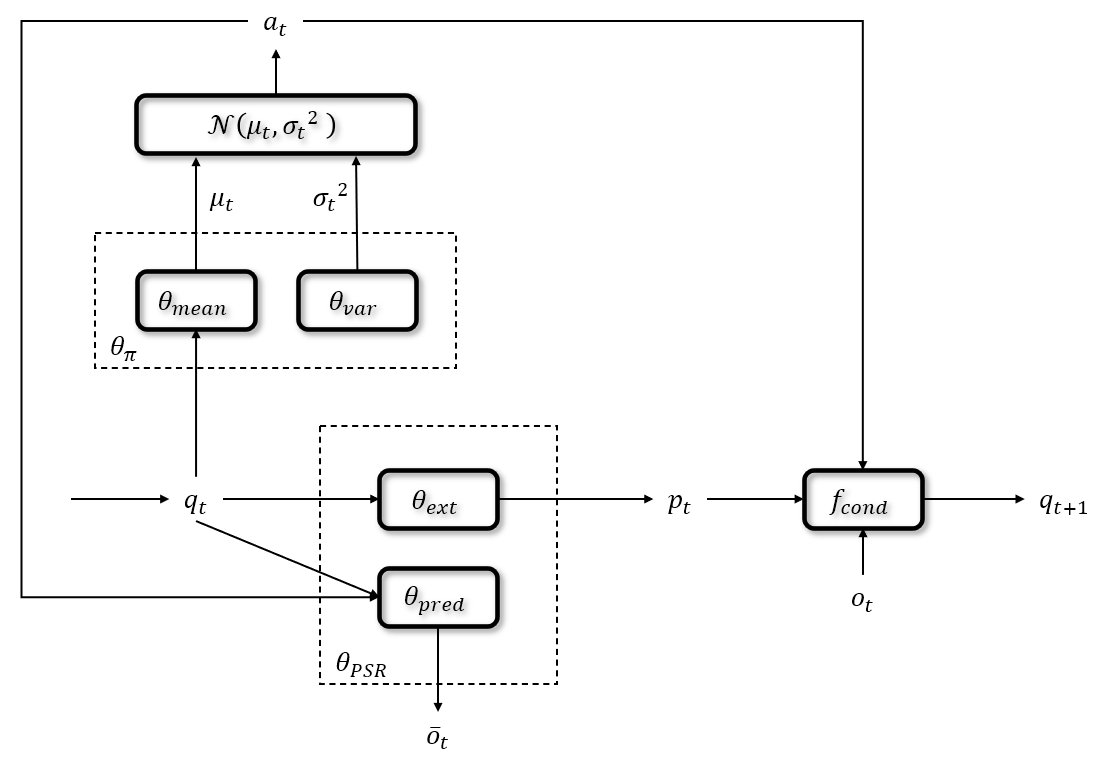
\includegraphics[width=15cm, keepaspectratio]{images/pomdp/pomdp_rpsp.png}
                    \caption{Recurrent Predictive State Policy network schema.}
                    \label{fig:pomdp_rpsp}
                \end{figure}
                
        \newpage        
        \subsection{DMDP Advantages over POMDP}
            In this section, the similarities between DMDP and POMDP frameworks have been highlighted, along with two architectures and two algorithms that aims to overcome the primary issues of exploiting Recurrent networks to solve POMDP problems. The fact that DMDPs can be seen as a particular case of POMDPs is very helpful towards the DMDP research field: POMDP research becomes a source of concepts, ideas and algorithms that could improve the DMDP state-of-the-art algorithms, while DMDP research remains scarce in general. At the same time, it highlights how DMDP problems may be as complex as POMDP problems in general. \newline
            However, DMDP framework has one significant advantage. While POMDP algorithms that are based on Predictive-State Representation models are forced to predict observations $o$ rather than states, due to the fact that usually in the POMDP framework states of the environment are not available, DMDP algorithms have access to the exact state $s$ after a certain number of steps, decided by the amount of delay present. At training time, Model-Based DMDP algorithms are able to optimize their state representations $\bar{s}$ by using the exact knowledge of the actually visited states $s$, rather than an inexact observation: it suffices to draw some trajectories using the currently learnt policy, collect the actually visited states and realign them with their correspondent prediction states. This procedure has already been tested by other researches such as \pcite{delay:ssbm} (Section \ref{subsub:modelbased_recurrent}) and the current research is based on the hypothesis that it is worth investigating in this direction in order to formulate new and better algorithms to solve the DMDP problems.
            
    \chapter{Preliminaries of the Research}
    \label{chap:prel}
    After having presented the advanced state-of-the-art knowledge upon which this research thesis is based, Chapter \ref{chap:prel} serves the purpose of discussing algorithms, architectures and techniques that have been used to implement the original network or that have been deployed alongside it. Section \ref{sota:trpo} is focused on the state-of-the-art RL algorithm that is deployed alonside the original network to carry out the action selection process, Trust Region Policy Optimization. In Section \ref{sota:selfan} the Transformer's architecture is presented, since its core mechanism, Self-Attention, has been adopted for the original implementation. At last, Section \ref{prel:maf} is focused on presenting Masked Autoregressive Flow, a density estimation technique that is used to train the original network, in such a way that makes it able to provide a belief distribution estimation of the current but unobserved state of the Agent.
    
    \section{Trust Region Policy Optimization}
        \label{sota:trpo}
        This section is dedicated to the presentation of the Trust Region Policy Optimization (TRPO) algorithm. As explained in Section \ref{subs:modelbasedapproach}, the goal of this research work is to define a module that is able to produce an efficient and meaningful state representation starting from the knowledge available to the Agent. However, the module needs to be coupled with a Reinforcement Learning algorithm in order to be deployed. In this regard, TRPO algorithm has been chosen as Reinforcement Learning algorithm due to its remarkable performances in a wide range of Environments. \newline
        TRPO is a gradient-based actor-critic Reinforcement Learning algorithm, presented by \pcite{trpo} with the goal of providing an efficient method to optimize nonlinear policies composed by a very high number of parameters, thus naturally including neural networks. The algorithm is based on theoretical results, which will be presented first, and it is build by approximating these results in order to reach a practical and implementable procedure, which is presented later as the actual algorithm.
        
        \subsection{Policy Gradient and Actor-Critic Methods}
        \label{subs:policygrad_actorcritic}
            \subsubsection{Policy Gradient Methods}
                % Policy Gradient explanation
                % Action-Value Method comparison
                Policy Gradient methods are a particular class of Reinforcement Learning algorithms that are focused on learning a parameterized policy, rather than an action-value or value function. Given a MDP $\langle \mathbf{S}, \mathbf{A}, p, \mathbf{R}\rangle$, a parameterized policy is defined as follows:
                
                \begin{definition}[Parameterized Policy $\pi_\theta$]
                    \label{def:parameterizedpi}
                    A Policy function $\pi$ is said to be parameterized w.r.t. a parameter vector $\theta \in \mathbb{R}^d$, where $d$ is the number of parameters, if $\pi$ is differentiable w.r.t. $\theta$. The parameterized policy function is denoted by $\pi(a|s, \theta)$ or simply $\pi_\theta$.
                \end{definition}
                
                As a result, $\pi(a|s, \theta)$ denotes the probability that action $a \in \mathbf{A}$ is selected in the environment state $s \in \mathbf{S}$ by policy $\pi$ with parameters $\theta$. The specific property that characterizes Policy Gradient methods is that, given a set of parameters $\theta$, the policy function $\pi$ does not need a value function $v_\pi$ or an action-value function $q_\pi$ in order to carry out the action selection. In practice, this means that given a state $s$, the $\pi$ is alone able to output an action $a$, without the need of "looking-up" to $v_\pi$ or $q_\pi$ in order to select it and only using  $\theta$ during the computation. In general $v_\pi$ or $q_\pi$ may be still used during the learning process in order to select a meaningful parameter vector $\theta$. \newline
                This is opposed to all methods and algorithms presented so far in previous chapters and sections, which aim at estimating an action-value function $q_\pi$ or a value function $v_\pi$ whose evaluations provide direct guidance for the action selection. Without them, the policy is unable to provide the next action. This class of algorithm is instead called Value-based methods.
                \\\\
                In general, a performance measure $J$ of the Agent in the Environment is defined as a function of the parameter vector $\theta$. The Agent's task is to find the parameter vector $\theta^*$ such that the performance of $J(\theta)$ is maximized when $\theta = \theta^*$. This task is directly mapped to a mathematical optimization problem such as the following:
                
                \begin{align*}  
                    \theta^{*} =    &\max_{\theta} J(\theta) \\
                \end{align*}
                
                which solution $\theta^*$ is the set of parameters such that the Agent that follows policy $\pi_{\theta^*}$ behaves optimally w.r.t. $J(\theta)$. In order to solve the previous optimization problem, Policy Gradient algorithms iteratively update the parameter vector $\theta$ through a gradient ascent update in $J$:
                
                \[ \theta_{t+1} = \theta_{t} + \alpha * \widehat{\nabla J(\theta_{t})} \]
                
                where $\widehat{\nabla J(\theta_{t})}$ is an estimation whose expectation approximates the gradient of the performance measure $J$ w.r.t. the parameter vector $\theta$ and $\alpha$ is the learning rate. \newline
                As an historical and meaningful example, for their REINFORCE algorithm, \pcite{REINFORCE} proposed as a performance measure $J$ the expected return of a parameterized policy $\pi_\theta$ written as the expectation over all possible trajectories $\mathbb{T}$:
                
                \[ J(\theta) = \int_{\mathbb{T}} p_{\theta}(\tau) R(\tau) d\tau \]
                
                where $\tau$ is a single possible trajectory, $p_{\theta}(\tau) = p(\tau|\theta)$ is the probability of trajectory $\tau$ to be drawn from a policy $\pi_{\theta}$ and $R(\tau)$ is the discounted reward collected in trajectory $\tau$. As a consequence, the $J(\theta)$ gradient is defined as follows:
                \[ \nabla_{\theta} J(\theta) = \int_{\mathbb{T}} \nabla_{\theta} p_{\theta} (\tau) R(\tau) d\tau = E \left[ \nabla_{\theta} \log p_{\theta}(\tau) R(\tau) \right]\]
                By further observing and proving that:
                \[ \nabla_{\theta} \log p_{\theta}(\tau) = \sum_{t=0}^{T} \nabla_{\theta} \log \pi_\theta (a_t | s_t) \]
                where T is the Time Horizon of trajectory $\tau$, \pcite{REINFORCE} also avoid the computational burden of estimating $p_{\theta}$ for each trajectory in order to compute $\nabla_{\theta} \log p_{\theta}$. Thus, the gradient $\nabla_{\theta} J(\theta)$ can be estimated without bias through collecting trajectories interacting in the environment and used to update $\theta$ with the foremention gradient ascent update.
                \\\\
                In general, proper optimization algorithms can be used to solve the defined problem, such as Conjugate Gradient or BFGS. The specific definitions of the performance measure $J$, the problem's constraints and the optimization algorithm chosen to solve this problem are properties of the specific algorithms that belongs to the Policy Gradient category. However, even when applied to examples where the gradient can be estimated accurately, Policy Gradient methods have demonstrated to be unsuccessful to reach good performances. The reason of this unsatisfying behaviour lies in both the high variance in the gradient estimate and in the greedy approach that Policy Gradient methods have shown, reducing the exploration rate very quickly to favor immediate reward gains, which in turn causes a very slow convergence to the optimum. 
                
            \subsubsection{Actor-Critic Methods}    
                In order to overcome the issues of Policy Gradient methods, several solutions and improvements have been proposed during the years. Important examples of this solutions are the following:
                \begin{itemize}
                    \item The adoption of a constant baseline $b$ in the policy gradient estimate (\pcite{REINFORCE}) in order to reduce its variance:
                    \[ \nabla_{\theta} J(\theta) = E \left[ \nabla_{\theta} \log p_{\theta}(\tau) R(\tau) \right] \]
                    \item  A different method to estimate the update step of the parameter vector $\theta$ in order to allow larger and safe updates to avoid the slow convergence of classical methods. This method is based on forcing the difference between the old trajectory distribution $p_{\theta}(\tau)$ and the new trajectory distribution $p_{\theta + \Delta\theta}(\tau)$ to be equal to an arbitrary value $\epsilon$, which leads to the definition of a different optimization problem:
                    \begin{align*}  
                        \max_{\Delta\theta} J(\theta + \Delta\theta) \approx J (\theta) + \Delta\theta^{T}\nabla_{\theta}J\\
                        \text{s. t. } \epsilon = D_{KL} \left( p_{\theta}(\tau)||p_{\theta + \Delta\theta}(\tau)\right) \\
                    \end{align*}
                    where $D_{KL}$ is the Kullback-Leibler divergence distance.
                \end{itemize}
                Subsequent research and studies around the problem of overcoming the inefficiency of Policy Gradient method eventually lead to a new class of Reinforcement Learning algorithms, Actor-Critic Methods. This class of methods inherits the properties of Policy Gradient methods, while adding a well-defined guidance procedure for the policy parameters $\theta$ improvements. \newline
                In Actor-Critic methods, the Actor is represented by the policy $\pi_\theta$, which inherits all properties from Policy Gradient methods. In addition, a Critic is chosen to evaluate the current policy $\pi_\theta$ and provide a basis for its improvement, i.e. it is directly involved in the computation of $\Delta\theta$. A common example of Critic is the state-value function $v_{\pi_{\theta}}$, which is updated along-side the policy function $\pi_\theta$ through bootstrapping during the learning process. The introduction of bootstrapping is a particularly important difference w.r.t. the Policy Gradient methods, since it introduces bias within the estimation of the gradient $\nabla_{\theta}J$. Infact, the bias introduced in Actor-Critic methods has been proved beneficial for the overall performances of the algorithms w.r.t. Policy Gradient methods, lowering the amount of variance in the estimate and accelerating the learning process. \newline
                
        \newpage
        \subsection{Theoretical Background}
        \label{subs:theoretical_background}
            \subsubsection{Theoretical Results}
                A few useful definition can be given to support the rest of the presentation. Consider a Markov Decision Process $\langle \mathbf{S}, \mathbf{A}, p, \mathbf{R}\rangle$ and a stochastic policy $\pi : \mathbf{S} \times \mathbf{A} \rightarrow [0, 1]$.
                
                \begin{definition}[Policy Expected Discounted Return $\mathbf{R^{\pi}}$]
                    \label{def:policyreturn}
                    The Policy Expected Discount Return $\mathbf{R^{\pi}}$ is defined as follows:
                    \[ \mathbf{R^{\pi}} =  \mathbf{E}_{\pi} \left[ \sum_{t=0}^\infty \gamma^t r_{t} \right] \]
                    where the expectation is taken w.r.t. all the possible trajectories that can be produced by an Agent that follows the policy $\pi$, $\gamma$ is the discount factor associated to the MDP and $r_t$ is the reward perceived at time-step $t$.
                \end{definition}
                
                Policy Expected Discounted Return $\mathbf{R^{\pi}}$ can be seen as the expectation over all possible Discounted Return $\mathbf{R_{0}^{\pi}}$ (Definition \ref{def:return}) and it is a key measure to define the performance of a given policy and to compare two different given policies, since it acts as an index for its global performance in the environment.
                
                \begin{definition}[Advantage Function $A_{\pi}$]
                    \label{def:advantagefunction}
                    The Advantage Function $A_{\pi}$ is defined as follows:
                    \[ A_{\pi}\left(s, a\right) = q_{\pi}\left(s, a\right) - v_{\pi}\left(s\right) \]
                    for each couple $(s, a)$ where $s \in \mathbf{S}$ and $a \in \mathbf{A}$, $q_{\pi}$ is the Action-Value function and $v_{\pi}$ is the Value Function related to policy $\pi$.
                \end{definition}
                
                The Advantage Function $A_{\pi}$ expresses the difference between the expected return of choosing a particular action $a$ in state $s$, $q_{\pi}(s, a)$, and the expected return of following $\pi$, thus choosing action $\pi(s)$ in state $s$, $v_{\pi}(s)$. In particular, the generic action $a$ may be provided by another policy $\pi'$, which implies that $a = \pi'(s)$. Intuitively speaking, the Advantage Function evaluated using action chosen by another policy $\pi'$ is a practical mean of comparison between the two policies, in order to establish which of the two policies behaves better in which states of the State Space and, in general, which policy is better than the other. This intuition is taken into action by \pcite{kakade2002}, which provides proof of the following identity:
                
                \[ \mathbf{R^{\pi'}} = \mathbf{R^{\pi}} + \mathbf{E}_{\pi'} \left[ \sum_{t=0}^\infty \gamma^t A_{\pi}\left(s_t, a_t\right) \right] \]
                
                where the expectation is taken over all the possible trajectories drawn by policy $\pi'$, meaning that the sequence of actions is chosen by $\pi'$, but the advantage function is computed w.r.t. policy $\pi$. Thus each evaluation of the advantage function indicates whether action $a_t = \pi'(s_t)$ is a better alternative to $\pi(s_t)$ or not and the whole expectation component of the identity can be considered as a delta of performance between $\pi$ and $\pi'$. By "unrolling" the expectation, the same identity can be rewritten as: 
                
                \[ \mathbf{R^{\pi'}} = \mathbf{R^{\pi}} + \sum_{s \in \mathbf{S}} \rho_{\pi'}(s) \sum_{a \in \mathbf{A}} \pi'(a|s) A_{\pi}(s,a) \]
            
                \[ where \; \;\rho_{\pi'}(s) = \sum_{t=0}^{\infty} \gamma^t P(s_t = s)\]
                
                In theory, starting from a given $\pi$ and optimizing $\mathbf{R^{\pi'}}$ as a function of $\pi'$ will yield a better policy as a result, but the complex dependency between $\pi'$ and $\rho_{\pi'}(s)$ makes it inaccessible from the optimization point of view. The next theoretical results aim at defining an approximation of $\mathbf{R^{\pi'}}$ that is tractable and at coping with the consequences of using an approximation instead of the actual measure.
                \\\\
                % Second theoretical results from Kakade
                Another important result presented and proved by \pcite{kakade2002} allows for simplifying the problem to a point in which it is tractable in practice. Infact, consider a parameterized policy $\pi_\theta$ and the following local approximation of $\mathbf{R^{\pi'}}$:
                
                \begin{definition}[Local Approximation of $\mathbf{R^{\pi'}}$]
                    \label{def:r_approximated}
                    \[ \mathbf{L^{\pi}(\pi')} = \mathbf{R^{\pi}} + \sum_{s \in \mathbf{S}} \rho_{\pi}(s) \sum_{a \in \mathbf{A}} \pi'(a|s) A_{\pi}(s,a) \]
                \end{definition}
                
                in which $\rho_{\pi'}(s)$ has been substituted with $\rho_{\pi}(s)$, thus ignoring the change in the visitation frequency of the states between $\pi'$ and $\pi$. Then, it holds:
                
                \begin{align}
                    \mathbf{L^{\pi_\theta}(\pi_{\theta_0})} &= \mathbf{R^{\pi_{\theta_0}}}\\
                    \nabla_\theta \mathbf{L^{\pi_\theta}(\pi_\theta)} \biggr\rvert_{\theta = \theta_0} &= \nabla_\theta \mathbf{R^{\pi_\theta}} \biggr\rvert_{\theta = \theta_0}\nonumber
                \end{align}
                
                for any parameter vector values $\theta_0$. This result is extremely remarkable: the approximation function $\mathbf{L^{\pi}}$ is equivalent to the approximated function $\mathbf{R^{\pi}}$ in first order derivation. Thus, for any sufficiently small step in the Policy Space such that $\mathbf{L^{\pi}}$ improves, improvement for $\mathbf{R^{\pi}}$ is guaranteed. Even more, $\mathbf{L^{\pi}}$ has been built by removing the complex dependence between $\pi$ and $\rho_{\pi}(s)$ that characterizes the definition of $\mathbf{R^{\pi}}$.
                \\\\
                % Theoretical Results from Schulman
                Thus the following step is to define a lower bound in order to describe how the actual performance measure $\mathbf{R^{\pi}}$ is linked to its approximation $\mathbf{L^{\pi}}$. This is provided and proved by \pcite{trpo} in the following theorem:
                
                \begin{theorem}[$D_{TV}$ Lower Bound on $\mathbf{R^{\pi}}$]
                    \label{th:trpo_dtvbound}
                    The following lower bounds holds for any couple of stochastic policies $\pi_{old}$ and $\pi_{new}$:
                    
                    \[ \mathbf{R^{\pi_{new}}} \geq \mathbf{L^{\pi_{old}}}(\pi_{new}) - \frac{4 \epsilon \gamma}{\left( 1 - \gamma \right)^2} D_{TV}^{max}(\pi_{old}, \pi_{new})^2\]
                    %
                    where:
                    \begin{itemize}
                        \item $\epsilon = \max_{s, a} | A_{\pi_{old}}(s, a) |$;
                        \item $\gamma \text{ is the discount factor associated to the MDP}$;
                        \item $D_{TV}^{max}(\pi_{old}, \pi_{new}) = \max_{s} D_{TV} (\pi_{old}(\cdot | s) || \pi_{new}(\cdot | s))$;
                    \end{itemize}
                    %
                    $D_{TV}$ is the usual definition of Total Variation Divergence between two probability distributions $p, q$: $D_{TV} (p,q) = \frac{1}{2} \sum_{i} | p_i - q_i |$.
                \end{theorem}
                
                Notice that the two policies $\pi$ and $\pi'$ are now denoted as $\pi_{old}$ and $\pi_{new}$ respectively, since it is of interest to apply the theoretical results presented so far in a context in which an optimization algorithm is able to find a new and better policy starting from a known, old one. Infact, the next and final theorem provided by \pcite{trpo} aim at defining an algorithm that is guaranteed to provide monotonic improvement at each iteration w.r.t. policy performance $\mathbf{R^{\pi}}$. \newline
                In order to proceed, the next well-known result is borrowed. Given two different probability distribution $p$ and $q$, it holds:
                
                \[ D_{TV} (p || q)^2 \leq D_{KL} (p || q)\]
                
                where $D_{KL}$ is the Kullback-Leibler Divergence between two probability distribution. Thus the following theorem becomes immediately available as a consequence of Theorem \ref{th:trpo_dtvbound}:
                
                \begin{theorem}[$D_{KL}$ Lower Bound on $\mathbf{R^{\pi}}$]
                    \label{th:trpo_dklbound}
                    The following lower bounds holds for any couple of stochastic policies $\pi_{old}$ and $\pi_{new}$:
                    
                    \[ \mathbf{R^{\pi_{new}}} \geq \mathbf{L^{\pi_{old}}}(\pi_{new}) - \frac{4 \epsilon \gamma}{\left( 1 - \gamma \right)^2} D_{KL}^{max}(\pi_{old}, \pi_{new})\]
                    %
                    where:
                    \begin{itemize}
                        \item $\epsilon = \max_{s, a} | A_{\pi_{old}}(s, a) |$;
                        \item $\gamma \text{ is the discount factor associated to the MDP}$;
                        \item $D_{KL}^{max}(\pi_{old}, \pi_{new}) = \max_{s} D_{KL} (\pi_{old}(\cdot | s) || \pi_{new} (\cdot||s))$;
                    \end{itemize}
                \end{theorem}
                \noindent
                Therefore the lower bound between the actual performance of the new policy $\pi_{new}$ and the approximated performance of the current policy $\pi_{old}$ is proportional to two main factors:
                
                \begin{itemize}
                    \item $\max_{s, a} | A_{\pi_{old}}(s, a) |$, which represents the maximum possible difference in expected return between $\pi_{old}$ and any other policy that chooses action $a$ in state $s$, with $(s,a) = \argmax_{s,a} | A_{\pi_{old}}(s, a) |$ while being equivalent to $\pi_{old}$ in other action selection;
                    \item $D_{KL}^{max}(\pi_{old}, \pi_{new})$, which represents the maximum difference in action selection probability distributions between the new policy $\pi_{new}$ and the old one $\pi_{old}$ between all states $s$.
                \end{itemize}
                \noindent
                Notice that the first term of the two becomes a constant in the context in which $\pi_{old}$ is given, for example as a result of the previous iteration of an algorithm, thus the lower bound becomes dependent only on $D_{KL}^{max}$, which infact will have a key role in the final TRPO algorithm.
                
            \subsubsection{Theoretical Algorithm}
            \begin{algorithm}[t]
                \SetAlgoLined
                \KwResult{Optimal Policy $\pi^{*}$}
                Initialize a random policy $\pi_{0}$\;
                Initialize converged = False\;
                \While{ \textbf{not} converged}{
                    Compute the Advantage Function $A_{\pi_{i}}$ for each couple $(s, a)$\;
                    Compute $\pi_{i+1}$ by solving the following Optimization Problem:
                    \begin{equation} 
                        \label{eq:trpo_opt}
                        \pi_{i+1} = \argmax_{\pi} \left[ \mathbf{L^{\pi_{i}}}(\pi)- \frac{4 \epsilon \gamma}{\left( 1 - \gamma \right)^2} D_{KL}^{max}(\pi_{i}, \pi)\right]
                    \end{equation}
                    \uIf{$\pi_{i+1} == \pi_{i}$} {
                        converged = True \;
                    }
                    
                }
                \caption{Policy Iteration based on Theorem \ref{th:trpo_dklbound}}
                \label{algo:trpo_dklbound}
            \end{algorithm}
                
                At last, it is now possible to define a theoretical algorithm that exploits Theorem \ref{th:trpo_dklbound} and it can be proven that it provides monotonic improvements w.r.t. the performance measure $\mathbf{R^{\pi}}$. The algorithm is presented in Algorithm \ref{algo:trpo_dklbound} and it consists of a Policy Iteration algorithm that bases the policy update upon the mentioned theorem. Consider an iteration $i$ of Algorithm \ref{algo:trpo_dklbound}, it is easy to observe that:

                \begin{equation}
                \label{eq:trpo_dklalgo_0}
                    D_{KL}^{max}(\pi_{i}, \pi_{i}) = 0
                \end{equation}
                \begin{equation} 
                    \label{eq:trpo_dklalgo_1}
                    \mathbf{R^{\pi_{i}}} = \mathbf{L^{\pi_{i}}}(\pi_{i})
                \end{equation}
                %
                The first result follows from the definition of $D_{KL}$, while the second is a direct consequence of the definition of $\mathbf{L^{\pi}}$ (Definition \ref{def:r_approximated}). Applying Theorem \ref{th:trpo_dklbound} to policies $\pi_{i}$ and $\pi_{i+1}$, with $\pi_{i+1}$ obtained from $\pi_{i}$ after one iteration of the algorithm:
                
                \begin{equation}
                    \label{eq:trpo_dklalgo_2}
                    \mathbf{R^{\pi_{i+1}}} \geq \mathbf{L^{\pi_{i}}}(\pi_{i+1}) - \frac{4 \epsilon \gamma}{\left( 1 - \gamma \right)^2} D_{KL}^{max}(\pi_{i}, \pi_{i+1})
                \end{equation}
                
                Subtracting Equation \ref{eq:trpo_dklalgo_1} to Disequation \ref{eq:trpo_dklalgo_2}, the following disequation is immediately obtained:
                
                \begin{equation}
                    \label{eq:trpo_dklalgo_3}
                    \mathbf{R^{\pi_{i+1}}} - \mathbf{R^{\pi_{i}}} \geq \left[ \mathbf{L^{\pi_{i}}}(\pi_{i+1}) - \frac{4 \epsilon \gamma}{\left( 1 - \gamma \right)^2} D_{KL}^{max}(\pi_{i}, \pi_{i+1}) \right] - \mathbf{L^{\pi_{i}}}(\pi_{i})
                \end{equation}
                
                The right-hand side of this disequation is always non-negative, infact $\pi_{i+1}$ is the policy that maximizes the quantity between the square brackets, thus by definition it is greater than $\mathbf{L^{\pi_{i}}}(\pi_{i})$. Therefore also $\mathbf{R^{\pi_{i+1}}} - \mathbf{R^{\pi_{i}}}$ is always a non-negative quantity, which proves that each iteration of Algorithm \ref{algo:trpo_dklbound} produces a policy $\pi_{i+1}$ that is better than or equal to $\pi_{i}$ w.r.t. the performance measure $\mathbf{R}$. In general, Algorithm \ref{algo:trpo_dklbound} produces a sequence of policies $(\pi_{0}, \pi_{1}, ..., \pi_{i}, ...)$ such that:
                
                \begin{equation}
                    \label{eq:trpo_dklalgo_4}
                    \mathbf{R^{\pi_{0}}} \leq \mathbf{R^{\pi_{1}}} \leq ... \leq \mathbf{R^{\pi_{i}}} \leq ...
                \end{equation}
                %
                until convergence to the optimal policy $\pi^*$ is reached. \newline
                The results presented so far, including the proof of  monotonic improvement of policy performances, are key aspects of the theoretical grounds for Trust Region Policy Optimization, which is designed to be a practical and meaningful approximation of Algorithm \ref{algo:trpo_dklbound}.
        
        \subsection{Formulation of the Algorithm}
        \label{subs:trpo_algorithm}
            In Section \ref{subs:theoretical_background}, a Policy Iteration algorithm (Algorithm \ref{algo:trpo_dklbound}) with the property of monotonic improvement at each iteration for a policy $\pi$ w.r.t. the performance measure $\mathbf{R^{\pi}}$. However, this algorithm serves as a theoretical background rather than an actual, implementable procedure, due to the fact that computationally infeasible assumption are implied:
            
            \begin{itemize}
                \item Policy Function $\pi$ is assumed evaluable at each state of the State Space, without further describing how the evaluation is carried out.
                \item Advantage Function $A_{\pi}$ is assumed known and available to be computed at each iteration for each couple $(s, a)$, while in practice it must be estimated from a finite number of samples gathered during the learning process;
                \item Optimization Problem \ref{eq:trpo_opt} is assumed to be solvable exactly at each iteration, while in practice approximations and heuristics must be applied in order to reduce its complexity and make it tractable.
            \end{itemize}
            
            In the next sections, practical solutions to these infeasible assumptions are presented, leading to the implementation of the TRPO algorithm proposed by \pcite{trpo}.
                
            \subsubsection{Theoretical and Heuristical Approximation}
                The definition of $\mathbf{L^{\pi}}$ and its properties (Definition \ref{def:r_approximated}) assume that policy $\pi$ is parameterized w.r.t. a certain vector $\theta \in \mathbb{R}^d$.  Thus, considering a parameterized policy $\pi_{\theta}$, the Optimization Problem \ref{eq:trpo_opt} can be rewritten in the space of the parameters vector $\theta$, rather than in the space of policies $\pi$:
                
                \begin{equation}
                    \label{eq:trpo_opt_theta}
                    \max_{\theta} \left[ \mathbf{L^{\pi_{\theta_{old}}}}(\pi_{\theta}) - C*D_{KL}^{max}(\pi_{\theta_{old}}, \pi_{\theta}\right)]
                \end{equation}
                %
                where the constants have been collapsed as follows:
                %
                \begin{itemize}
                    \item $C = \frac{4 \epsilon \gamma}{\left( 1 - \gamma \right)^2}$
                    \item $\epsilon = \max_{s, a} | A_{\pi_{\theta_{old}}}(s, a) |$
                \end{itemize}
                %
                However, the optimization problem prescribed by the theory still present some convergence speed issues: using the penalty coefficient $C$ as defined above, the step made by the policy parameter $\theta$ would be very small. Thus, in order to enlarge each steps while mantaining robusticity, the penalization on $\mathbf{L^{\pi_{\theta_{old}}}}(\pi_{\theta})$ can be trasformed into a constraint on the Kullback-Leibler divergence between the new and the old policy, which is called a Trust Region constraint. In practice, the optimization problem is reformulated as follows:
                
                \begin{align}
                    \label{eq:trpo_opt_theta_constraint}
                    &\max_{\theta} \mathbf{L^{\pi_{\theta_{old}}}}(\pi_{\theta}) \\
                    &\text{s. t. } D_{KL}^{max}(\pi_{\theta_{old}}, \pi_{\theta}) \leq \delta \nonumber
                \end{align}
                
                where $\delta$ is a hyper-parameter of the final algorithm. The next step towards a feasible optimization problem concerns the new constraint. Evaluating $D_{KL}^{max}(\pi_{\theta_{old}}, \pi_{\theta}) \leq \delta$ implies evaluating the constraint for each state in the state space $\mathbf{S}$, thus the constraint actually comprises a very large number of constraints, so large that it is actually infeasible in practice. A heuristic approximation is used to make the optimization problem tractable by substituting $D_{KL}^{max}$ with the average Kullback-Leibler divergence, $\bar{D}^{\rho_{old}}_{KL}$, defined as follows:
                
                \begin{definition}[Average KL Divergence $\bar{D}^{\rho}_{KL}$]
                    \label{def:avg_kl_div}
                    \[ \bar{D}^{\rho_{old}}_{KL} (\pi_{\theta_{old}}, \pi_{\theta_{new}}) = \mathbf{E}_{s\sim\rho_{old}} \left[ D_{KL} (\pi_{\theta_{old}}, \pi_{\theta_{new}}) \right]\]
                \end{definition}
                
                Optimization problem \ref{eq:trpo_opt_theta_constraint} is then reformulated accordingly with this definition as follows:
                
                \begin{align}
                    \label{eq:trpo_opt_theta_avgkl}
                    &\max_{\theta} \mathbf{L^{\pi_{\theta_{old}}}}(\pi_{\theta}) \\
                    &\text{s. t. } \bar{D}^{\rho_{old}}_{KL} (\pi_{\theta_{old}}, \pi_{\theta_{new}}) \leq \delta \nonumber
                \end{align}
                
                which represents a tractable optimization problem. Infact, this is the optimization problem that the Trust Region Policy Optimization algorithm aims to solve in order to learn a good parameter vector $\theta$. However, in order to actually solve it, the algorithm needs to take into account the fact that the advantage function $A_\pi$ is not given and must be estimated through samples gathered while interacting with the environment. The next section is concerned with solving this issue.
                
            \subsubsection{Sample-Based Estimation}
                % Formulating the actual maximization problem
                At first, it is possible to expand $\mathbf{L^{\pi_{\theta_{old}}}}(\pi_{\theta})$ accordingly to definition \ref{def:r_approximated}, rewriting the optimization problem as follows:
                
                \begin{align}
                    \label{eq:trpo_opt_L_expanded}
                    &\max_{\theta} \sum_{s \in \mathbf{S}} \rho_{\pi_{\theta_{old}}}(s) \sum_{a \in \mathbf{A}} \pi_{\theta}(a|s) A_{\pi_{old}}(s, a) \\
                    &\text{s. t. } \bar{D}^{\rho_{\pi_{\theta_{old}}}}_{KL} (\pi_{\theta_{old}}, \pi_{\theta_{new}}) \leq \delta \nonumber
                \end{align}
                
                where the $\mathbf{R}^{\pi_{\theta_{old}}}$ component has been removed, since it is constant w.r.t. the optimization variable $\theta$. Subsiquently, $\sum_{s \in \mathbf{S}} \rho_{\pi_{\theta_{old}}}(s)$ can be replaced with the expectation over the states drawn by policy $\pi_{old}$, as the sampling distribution, and $A_{\pi_{old}}(s, a)$ can be simplified with $q_{\pi_{old}}(s, a)$ by observing that $v_{\pi_{old}}(s)$ is a constant w.r.t. $\theta$:
                
                \begin{align}
                    \label{eq:trpo_opt_expectation}
                    &\max_{\theta} \mathbf{E}_{s\sim\rho_{\pi_{old}},\;a\sim\pi_{old}} \left[ \frac{\pi_{\theta}(a|s)}{\pi_{\theta_{old}}(s|a)} q_{\pi_{\theta_{old}}}(s,a)\right] \\
                    &\text{s. t. } \mathbf{E}_{s\sim\rho_{\pi_{\theta_{old}}}} \left[ D_{KL} ( \pi_{\theta_{old}}(\cdot|s) || \pi_{\theta} (\cdot|s) ) \right] \leq \delta \nonumber
                \end{align}
                
                where the objective function of the optimization problem and the action-value function $q_{\pi_{\theta_{old}}}$ can be approximated using Monte Carlo simulation. Furthermore, the objective function is named Surrogate Advantage function and it will be denoted as $\mathbf{\bar{L}^{\pi_{\theta_{old}}}}$. \newline
                In practice, a sequence of trajectories $(s_0, a_0, s_1, a_1, ..., s_T, a_T)$ drawn by policy $\pi_{\theta_{old}}$ is collected and $q_{\pi_{\theta_{old}}}$ is estimated at each pair $(s_t, a_t)$ with $t \in [0, T]$ by computing the discounted sum of future rewards collected along the trajectory. At the same time, expectations are approximated through sample averages.
                
            \subsubsection{Trust Region Policy Optimization Algorithm}
                % Actual Algorithm
                Finally, it is possible to enter in the details of how the algorithm is implemented, i.e. how Optimization Problem \ref{eq:trpo_opt_expectation} is iteratively solved. At each iteration of the algorithm, the gradient of the Surrogate Advantage function $\mathbf{\bar{L}^{\pi_{\theta_{old}}}}$ is approximated and an update is performed over the parameter vector $\theta$. In order to be able to iterate in an optimized and robust way, both the Surrogate Advantage function and the Trust Region constrain are Taylor expanded, respectively at the first and second order:
                
                \begin{align}
                    \mathbf{\bar{L}^{\pi_{\theta_{t}}}} &\approx g^{T}(\theta - \theta_{t})\\
                    D_{KL} ( \pi_{\theta_{t}}(\cdot|s) || \pi_{\theta} (\cdot|s) ) &\approx \frac{1}{2} (\theta - \theta_{t})^{T}H(\theta - \theta_{t})
                \end{align}
                
                where $g$ represents the $\mathbf{\bar{L}^{\pi_{\theta_{t}}}}$ gradient w.r.t. $\theta$ and likewise $H$ is its Hessian matrix. Observe that the subscript $old$ has been replaced by $t$, in light of the fact that subsequent optimization iterations are now taken into consideration. The optimization problem is again trasformed as follows:
                
                \begin{align}
                    \label{eq:trpo_opt_taylor}
                    \theta_{t+1} &= \argmax_{\theta} g^{T}(\theta - \theta_{t}) \\
                    & \text{s. t. } \frac{1}{2} (\theta - \theta_{t})^{T}H(\theta - \theta_{t}) \leq \delta \nonumber
                \end{align}
                
                Optimization Problem \ref{eq:trpo_opt_taylor} can be analytically solved using Lagrangian Duality methods, which bring to the following solution:
                
                \[ \theta_{t+1} = \theta_{t} + \sqrt{\frac{2\delta}{g^{T}H^{-1}g}} H^{-1}g\]
                
                However, this solution may not satisfy the original Trust Region constraint or even lead to a positive Surrogate Advantage due to the approximation introduced by the Taylor expansion. Thus, TRPO solves this issue by adding a Backtracking Line Search as follows:
                
                \[ \theta_{t+1} = \theta_{t} + \alpha^{j} \sqrt{\frac{2\delta}{g^{T}H^{-1}g}} H^{-1}g\]
                
                with $\alpha \in (0, 1)$ as backtracking coefficient and $j \geq 0 \in \mathbb{N}$ as the smallest nonnegative integer such that the solution produced is both satisfying the Trust Region constraint and resulting in a positive Surrogate Advantage. \newline
                The last step towards the final algorithm is defining an optimized way to compute the inverse matrix $H^{-1}$, which dimensions can easily become intractable when the parameter vector $\theta$ is large, as in the case of neural networks used as policy functions. The solution adopted by TRPO algorithm is to actually compute the quantity $H^{-1}g$ alltogether, which can be done in a relatively fast way by solving the optimization problem $Hx = g$ using Conjugate Gradient optimization method. The TRPO algorihm is presented in Algorithm \ref{algo:trpo}.
                
                \newpage
                \begin{algorithm}[h]
                    \SetAlgoLined
                    \KwResult{Optimal Policy $\pi_{\theta^*}$}
                    Initialize policy parameter vector $\theta_0$\;
                    Initialize value function parameter vector $\phi_0$\;
                    Initialize the following hyperparameters: Trust Region contraint $\delta$, backtracking coefficiency $\alpha$ and max number of backtracking step $\bar{j}$\;
                    Initialize number of epochs, $T$, the current epoch $t=0$  and the maximum number of steps of each episode $I$\;
                    \While{$t \leq T$}{
                        Retrieve a set of trajectories $\mathbb{T}_{t}$ by letting the current policy $\pi_{\theta_{t}}$ interact with the environment\;
                        Compute the rewards-to-go $\bar{R}_i$ for each step of each trajectory\;
                        Compute the Advantage Function estimate $\bar{A}_t$ for each step of each trajectory, based on the current value function $V_{\phi_{t}}$\;
                        Policy Gradient estimation:
                        \[ \bar{g}_t = \frac{1}{|\mathbb{T}_{t}|} \sum_{\tau \in \mathbb{T}_{t}} \sum^{I}_{i=0} \nabla_{\theta_{t}} \log \pi_{\theta_{t}} (a_i|s_i) \bar{A}_t; \;\]
                        Gradient and inverse Hessian matrix product by conjugate gradient:
                        \[ \bar{x}_{t} \approx \bar{H}^{-1}_{t} \bar{g}_t; \;\] 
                        Policy parameter update through backtracking line search:
                        \[ \theta_{t+1} = \theta_{t} + \alpha^{j} \sqrt{\frac{2\delta}{\bar{g}_{t}^{T} \bar{x}_{t}}} \bar{x}_{t} \]
                        where $j$ is chosen accordingly with the backtracking line search \;
                        Value function regression against the computed rewards-to-go:
                        \[ \phi_{t+1} = \argmin_{\phi} \frac{1}{|\mathbb{T_{t}}| T} \sum_{\tau \in \mathbb{T}_{t}} \sum_{i=0}^{I} \left( v_{\phi}(s_i) - \bar{R}_i \right)^{2}; \;\]
                        Update $t=t+1$\;
                    }
                    \caption{Trust Region Policy Optimization}
                    \label{algo:trpo}
                \end{algorithm}
    
    \newpage
    \section{Attention Network: Transformer}
    \label{sota:selfan}
        In this section, a fairly recent kind of neural networks is presented, the Transformer. Proposed by \pcite{an:transformer}, the Transformer network represents a new architecture which exploits self-attention mechanism alone in order to learn upon sequences of inputs, other than also relying on Recurrent or Convolutional mechanisms. The Transformer is able to cope with variable-length sequences of inputs without sacrificing potential parallel computing, as in the case of Recurrent models. For this reasons and given its ability to compete with other state-of-the-art models, it makes a suitable candidate in order to implement a network that is able to maintain internal state while being natively compatible with stochastic delays, that are bound to generate variable-length extended states.
        
        \subsection{Sequence-to-Sequence Models}
        \label{sub:seq2seq}
            \begin{figure}[b]
                    \centering
                    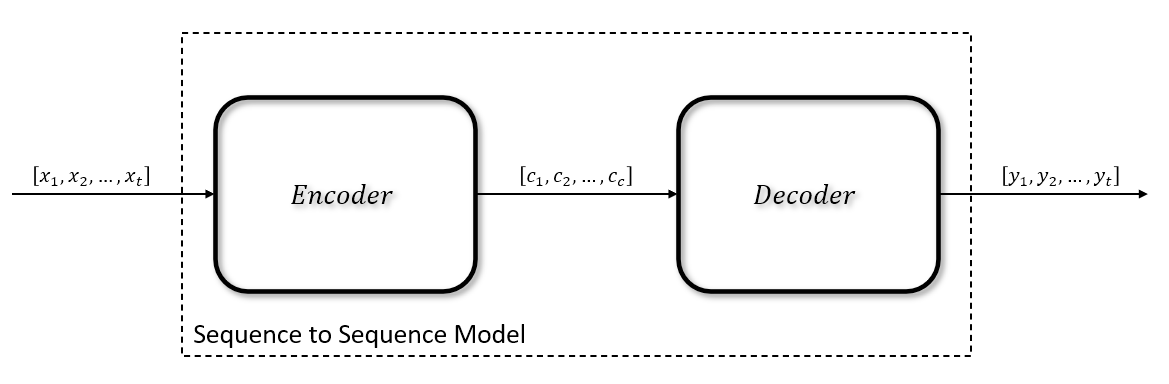
\includegraphics[width=15cm, keepaspectratio]{images/an/seq2seq.png}
                    \caption{High-level representation of a Sequence-to-Sequence model. The input sequence $\mathbf{x} = \left[x_1, x_2, ..., x_t \right]$ is encoded into a Context Vector $\mathbf{c} = \left[c_1, c_2, ..., c_d \right]$ which, in turn, is decoded into the output sequence $\mathbf{y} = \left[y_1, y_2, ..., y_t \right]$.}
                    \label{fig:an_seq2seq}
            \end{figure}
        
            Transformer's architecture is based on sequence-to-sequence model. Sequence-to-sequence models, often abbreviated as seq2seq, have been first presented by \pcite{an:seq2seq} and are specifically designed to process sequences of inputs in order to produce sequences of outputs. The overall model is composed of two main component: an Encoder, which elaborates the input sequences and encodes them into a Context Vector; and a Decoder, which elaborates the Context Vector and computes the output sequences. Figure \ref{fig:an_seq2seq} illustrates the architecture from a high-level perspective.\newline
            More precisely, Encoder and Decoder interact between each other in a sequential fashion, each of them is dedicated to one step of the translation from the input sequence $\mathbf{x} = [x_1, x_2, ..., x_t]$ to the output sequence $\mathbf{y} = \left[y_1, y_2, ..., y_t \right]$:
            \begin{itemize}[topsep=0.5em, partopsep=0.5em]
                \setlength\itemsep{0em}
                \item The Encoder $E$ takes as input the sequence $\mathbf{x} = [x_1, x_2, ..., x_i]$ and encodes it in an intermediate representation, the Context vector $\mathbf{c} = [ c_1, c_2, ..., c_c]$, which length is fixed and decided at the initialization of the overall model;
                \item The Decoder $D$ takes as input the Context vector $\mathbf{c} = [ c_1, c_2, ..., c_c]$ and decodes it into the output sequence $\mathbf{y} = \left[y_1, y_2, ..., y_{i'} \right]$.
            \end{itemize}
            
            Thus, the sequence produced by the model $\mathbf{y}$ can be compared to the actual output sequence $\mathbf{\tilde{y}}$ to compute a loss function upon which the entire model can be trained upon. \newline
            It is important to note that the lengths of input and output sequences are not fixed and may change from one sequence to the other in the same dataset. Similarly, correspondent input and output sequences may not have the same length. This properties imposes some constraints one which kind of networks can be used to implement Decoders and Encoders.
            
            \subsubsection{Recurrent Mechanism}
            \label{subsub:seq2seq_rnn}
                Sequence-to-sequence model have found applications in the context of Neural Machine Translation, the process of translating word and phrases from one language to another, and Image Captioning, the process of generating textual descriptions of images. Given the need of processing sequences of data, Recurrent neural networks are the prime candidate networks for effectively implementing Encoders and Decoders, along with Convolutional networks in order to deal with image representation. Infact, the original work on Sequence-to-Sequence models (\pcite{an:seq2seq}) refers to a Recurrent implementation for Encoders and Decoders, while another pioneer work such as \pcite{an:rnn} proposes an implementation by means of Long-Short Term Memories (LSTM, \pcite{dl:lstm}). \newline
                In general, exploiting Recurrent networks to implement Encoder and Decoder means that each element of the input and output sequences, respectively, is processed one at each time-step for the Recurrent network. If the input sequence contains $e$ elements, the Encoder needs $e$ time-steps to process them: at each time-step, it processes one element of the sequence and updates its internal state, $enc$. The last internal state is the context vector $\mathbf{c}$. If the output sequence contains $d$ elements, the Decoder needs $d$ time-step to produce them: at each-time step, it outputs one element of the output sequence $\mathbf{y}$ and updates its internal state, $dec$. Thus, the entire model needs $e+d$ time-step to process the input sequence and compute the correspondent output sequence.
                \\\\
                More specifically, details on how to update the internal states of Encoder and Decoders and how to condition the output of each Decoder timestep over the Context vector $\mathbf{c}$, previous internal state $enc$ or previous generated output element $y$ fall to the specific implementation design choices of a Sequence-to-sequence model. However, this particular Sequence-to-sequence model has shown two specific issues:
                \begin{itemize}[topsep=0.5em, partopsep=0.5em]
                    \setlength\itemsep{0em}
                    \item Systematic performance losses against longer input/output sequences, for example against longer sentences to be translated;
                    \item The sequential nature of the computation across Encoder and Decoder layers does not allow for efficient parallel computation, thus making the entire model hard to optimize.
                \end{itemize}
                
                        
            \subsubsection{Attention Mechanism}
            \label{subsub:attention_mechanism}
                In order to cope with performance issues regarding long sequences, \pcite{an:attention} propose a new mechanism, Attention, to be integrated within the current Sequence-to-sequence Recurrent models. \newline
                The Attention mechanism stems from the idea that having a fixed-length Context vector $\mathbf{c}$ can represent an important bottleneck for the network performances. Infact, regardless of the lengths of input and output sequences, the dimension of the Context vector and thus the amount of information that it can encode is limited and fixed. The introduction of Attention mechanism allows for modifying the interaction between the Encoder and the Decoder, towards a more complex and complete passage of information. In practice, the following modifications are applied to the Sequence-to-sequence model:
                
                \begin{itemize}[topsep=0.5em, partopsep=0.5em]
                    \setlength\itemsep{0em}
                    \item Attention Recurrent Encoder $E$: instead of passing only the last internal state $\mathbf{c}$, the Encoder keeps in memory the internal states $enc_i$ related to each element of the input sequence $\mathbf{x}$ and passes them along with the last one. The set of internal states is denoted as $\mathbf{enc}$. Thus the amount of encoded information that is available to the Decoder is larger;
                    \item Attention Recurrent Decoder $D$: At each time-step $i$, the Decoder network takes as input $\mathbf{enc}$, its own internal state $dec_i$ and the previous generated element of the output sequence $\mathbf{y}$ with the purpose of generating the next element, while updating $dec_i$.
                \end{itemize}
                
                The Attention mechanism relies in how the Decoder exploits the knowledge contained in the set of Encoder internal states $\mathbf{enc}$. At each time-step $i$, the Decoder executes the following steps:
                
                \begin{enumerate}[topsep=0.5em, partopsep=0.5em]
                    \setlength\itemsep{0em}
                    \item Scoring Function: each encoder internal state in $\mathbf{enc}$ is evaluated against the decoder internal state $dec_i$ in order to produce a score.
                    \item Softmax: the score results of the previous step are then passed through a Softmax layer to normalize the values;
                    \item Weighted average of the internal states in $\mathbf{enc}$ by their scores, the result of this passage represents the Context vector for time-step $i$, $\mathbf{c_i}$.
                \end{enumerate}
                
                The Context vector $\mathbf{c_i}$ along with the decoder internal state $dec_i$ is then passed through a Feedforward neural network to generate the actual output element. 
                \\\\
                The concept behind the Attention mechanism is simple: the Decoder has access to the full encoded information of the Decoder and autonomously decides on which part of information is worth "paying attention" to and when. This is done through scoring the encoder internal states against the decoder internal state. In this way, the Decoder is able to look for useful information also in other encoder internal states rather than in a fixed Context vector, which in turn means that it is able to relate information coming from different input elements at once, in order to generate the next output element. \newline
                This process revealed to be very beneficial in the context of Neural Machine Translation (NMT) as shown by \pcite{an:attention}, where paying attention to different words in different positions of the input sentence is a key factor in understanding which is the correct output word.
        
        \newpage      
        \subsection{Transformer Architecture}
        \label{sub:transformer}
        \begin{figure}[!t]
                \centering
                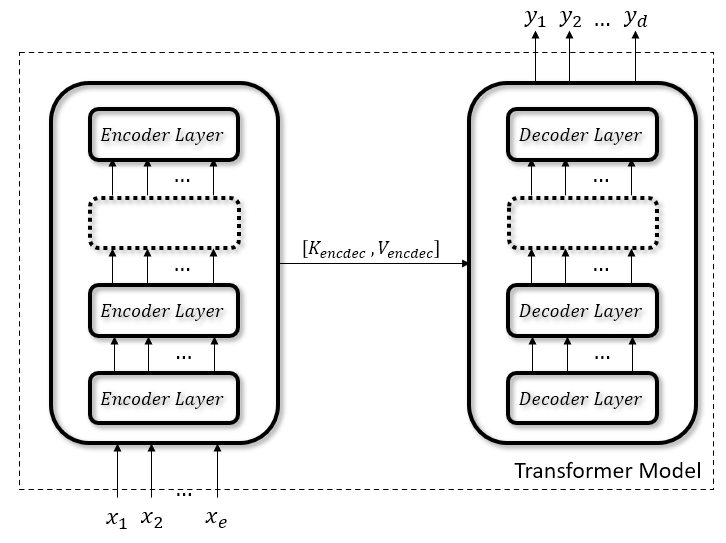
\includegraphics[width=15cm, keepaspectratio]{images/an/transformer.png}
                \caption{High-level representation of a Transformer model.}
                \label{fig:an_transformer}
        \end{figure}
        
            Transformer's architecture design choices stem from observing that while the application of the Attention mechanism on Sequence-to-sequence model has been beneficial performance-wise, the problem of having limited possibilities towards exploiting parallel computing still persists, since the core implementation of Encoders and Decoders remains the Recurrent mechanism. For this reason, Transformer's architecture aims at implementing an Attention mechanism only, called Self-Attention mechanism.\newline
            At first, it is important to highlight that the Encoder's and Decoder's structures of the Transformer is composed of several layer, respectively called Encoder layers and Decoder layers, instead of a single Recurrent network. The first Encoder layer takes as input the input sequence $\mathbf{x}$ and, sequentially, the following Encoder layers take as input the output of the previous layer. The last Encoder layer's output is used as input for each Decoder layer along with the previous Decoder's output. The last Decoder layer's output is the output sequence $\mathbf{y}$. Figure \ref{fig:an_transformer} illustrated the architecture from a high-level perspective. In order to further detail the structure of the Transformer, it is important to present how Encoder and Decoder layers function.
            
            \subsubsection{Positional Encoding}
        %       - Positional Encoding (Position in the sequence matters)
                Before processing the input sequence $\mathbf{x}$, the Transformer architecture allows for embedding information about the position of each element in the sequence, through a technique called Positional Encoding, presented by \pcite{an:transformer}.\newline
                For each position $i$ in the sequence $\mathbf{x}$, a positional vector $p_i$ of the same dimensions as $x_{i}$ is defined as follows:
                
                \begin{equation}
                    \label{eq:pos_enc}
                    p_{i}^{d} \coloneqq \begin{cases}
                                            \sin(\omega_k * t) & \text{if } d = 2k\\
                                            \cos(\omega_k * t) & \text{if } d = 2k + 1\\ 
                                        \end{cases}
                \end{equation}
                where $d$ represents each single dimension within the $p_i$ vector and $\omega_k$ is so defined:
                \[ \omega_k = \frac{1}{10000^{2k/d}} \]
                This definition leads to a $p_i$ vector built in the following way:
                
                \[ p_i \coloneqq \left[ \sin(\omega_1 * i), \cos(\omega_1 * i), \sin(\omega_2 * i), \cos(\omega_2 * i), ..., \sin(\omega_{d/2} * i), \cos(\omega_{d/2} * i)\right] \]
                \noindent
                Given the definition of $\omega_k$, $p_i$ represents a geometric progression from $2\pi$ to $10000*2\pi$ with decreasing frequencies along $p_i$ dimensions. In order to embed Positional Encoding into each element $x_{i}$, the sum of the two is computed: 
                
                \[ x_{i}^{pos} = x_{i} + p_i \]
                \noindent
                For simplicity of notation, $x_{i}^{pos}$ will still be denoted by $x_{i}$ in the rest of the section. 
            
            \subsubsection{Transformer Encoder}
            \label{subsub:trans_encoder}
                \begin{figure}[!t]
                    \centering
                    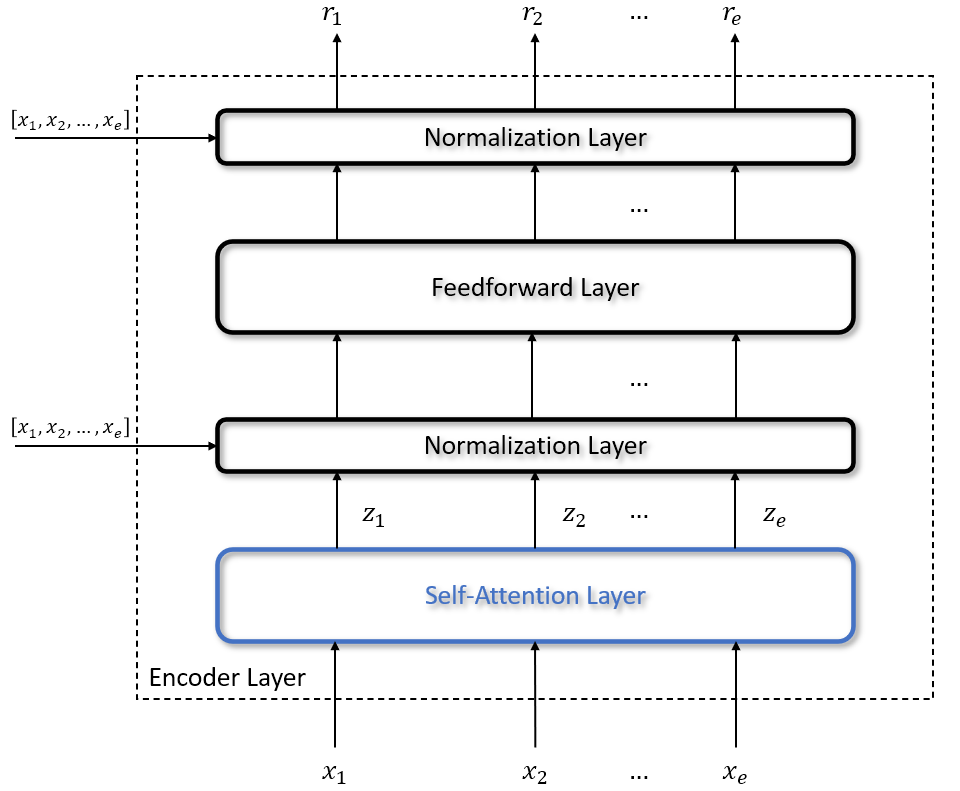
\includegraphics[width=15cm, keepaspectratio]{images/an/transformer_encoder.png}
                    \caption{High-level representation of a Transformer Encoder Layer model.}
                    \label{fig:an_transformer_encoder}
                \end{figure}
                
                Each Encoder layer presents the same structure composed of two subsequent sublayers: a Self-Attention layer and a Feedforward neural network. Thus, it is possible to analyze the behaviour of the first Encoder layer in order to generalize it later. \newline
                The Self-Attention layer is composed of three learnt parameters matrices: a Query Matrix $W_q$, a Key Matrix $W_k$ and a Value Matrix $W_v$. Each element of the input sequence $\mathbf{x} = [x_1, x_2, ..., x_e]$ is processed separately by the Self-Attention layer in the following sequence of computation:
                \begin{enumerate}
                    \item \textbf{Query, key and value projection}: each element $x_i$ is multiplied by $W_q$, $W_k$ and $W_v$ separately in order to produce the query vector $q_i$, the key vector $k_i$ and the value vector $v_i$.
                    \begin{align*} 
                        q_i &= x_i W_q\\
                        k_i &= x_i W_k\\
                        v_i &= x_i W_v\\
                    \end{align*}
                    Note that this computation requires each $x_i$ to have the same dimensions, otherwise the vector matrix product wouldn't be possible. In applications where this requisite is not available, such as Neural Machine Translation where each word cannot have the same length, techniques to reduce its element to a vector of fixed-size are exploit, such as Word Embedding techniques.
                    
                    \item \textbf{Score computation}: A score $s_{i, j}$ for each element in the input sequence $x_j$ is computed. The query vector $q_i$ is multiplied to each key vector $k_j$. The result is divided by the root square of the length of key vectors $l_k$ in order to normalized the values and all the scores are softmaxed so to retrieve values that add up to 1:
                    \[ s_{i,j} = \text{softmax} \left( \frac{q_i * k_j}{\sqrt{l_k}} \right) \]
                    
                    The meaning of this computation is to understand "how much attention" needs to be payed at all the elements of the sequence while processing $x_i$, allowing to keep track of possibly different elements $x_j$.
                    
                    \item \textbf{Value weighted average}: In order to compute the attention result vector $z_i$, the sum of each value vector $v_j$ weighted by the score $s_{i,j}$ is computed:
                    \[ z_i = \sum_{j=0}^e s_{i,j} * v_j \]
                    
                    Each value vector $v_j$ represents the encoded knowledge of the correspondend element $x_j$, thus the average weighted by the score represents a compact way of encoding the values of each element of the input sequence.
                    
                \end{enumerate}
                \noindent
                At this point, the Encoder layer has computed a sequence of Attention vectors $\mathbf{z} = [z_1, z_2, ..., z_e]$, which is then normalized through a Normalization Layer. Each element of $\mathbf{z}$ is then passed through the the Feedforward network, which parameters are learnt, and the results of the Encoder layer are produced, denoted as $\mathbf{r} = [r_1, r_2, ..., r_e]$. Figure \ref{fig:an_transformer_encoder} illustrates the architecture of one Encoder layer.\newline
                Since the Encoder layers structure remains the same throughout all layers, it is straightforward to generalize this behaviour to the entirety of the Encoder: the sequence of results $\mathbf{r_1}$ of the first layer is taken as input by the second layer, which in turn will produce a second sequence of results $\mathbf{r_2}$ taken as input by the third layer, and so on, until the last layer. \newline
                At last, the sequence of Encoder results $\mathbf{r_e}$ is used to produce a Key Matrix and a Value Matrix, respectively denoted as $K_{encdec}$ and $V_{encdec}$ which will be delivered to the Decoder of the Transformer.
            
            \subsubsection{Layer Normalization}
                Layer Normalization is a normalization technique that has been proposed by \pcite{dl:layernorm} with the purpose of reducing the training time of the network. In practice, the following computation is carried out on each element $x_{i}$ input to the Normalization layer:
                
                \begin{align}
                \label{eq:layer_norm}
                    x^{norm}_{i} = \frac{x_{i} - \mathbf{E} \left[ x_{i} \right]}{\sqrt{\mathbf{Var} \left[ x_{i} \right] + \epsilon}} * \gamma + \beta
                \end{align}
                
                where $\mathbf{E} \left[ x_{i} \right]$ and $\mathbf{Var} \left[ x_{i} \right]$ are estimated element-wise on the input batch the module is supplied with at each training process; $\epsilon$ represents a low value for numerical stability, usually set to $10^{-5}$, while $\gamma$ and $\beta$ represents learnable parameters of the Normalization Layer. \newline
                In the Transformer architecture, the Layer Normalization is computed on the summation between the input sequence $\mathbf{x}$ and the output sequence of the previous layer, for example the sequence of attention vectors $\mathbf{z}$. Denoting as $\mathbf{\tilde{z}}$ the sequence of normalized attention vectors:
                
                \begin{align*}
                    \tilde{z}_{i} = \frac{ (x_{i} + z_{i}) - \mathbf{E} \left[ (x_{i} + z_{i}) \right]}{\sqrt{\mathbf{Var} \left[ (x_{i} + z_{i}) \right] + \epsilon}} * \gamma + \beta
                \end{align*}
            
            \subsubsection{Input Sequence Mask}
                Before processing the sequence $\mathbf{x}$ through each Encoder layers, an optional computation within the network is provided: masking the input sequence. A mask is a matrix handled by the Encoder layer's implementation that masks out certain positions during the Self-Attention computation of each element $x_{i}$. In practice, for each element $x_{i}$, the mask specifies which elements of $\mathbf{x}$ are relevant by adding 0 to the Attention score computation within the $Softmax$ operator and which elements are not by adding $-\infty$. \newline
                The construction of the mask is handled specifically for each implementation of the Transformer and it can be used to embed specific information within the Self-Attention computation. For example, it is possible to embed temporal causality by masking out future positions elements in the self-attention computation of each input element, thus relating each element to its previous ones.
            
            \subsubsection{Transformer Decoder}
            \label{subsub:trans_decoder}
                Similarly to the Encoder's structure, the Decoder is composed of several layer with identical structure. In turn, each Decoder layer is composed of three subsequent sublayers: a Self-Attention layer, an Encoder-Decoder Attention layer and a Feedforward neural network. However, the Decoder does not process its input sequentially at once like the Encoder does: for each element in the output sequence $\mathbf{y}$, the Decoder processes only the output sequence produced so far, thus taking as input the sequence $\mathbf{\tilde{y}} = [y_1, y_2, ..., y_i-1]$ along with the matrices already produced by the Encoder, $K_{encdec}$ and $V_{encdec}$. This is achieved by masking "future" positions in the softmax operation within the Self-Attention layer. Once the Decoder has generated a specific output element that is used to signal the end of the sequence, the output sequence $\mathbf{y}$ is complete. \newline
                In practice, each Decoder layer functions in a similar way to an Encoder one, except for the presence of an Encoder-Decoder Attention layer:
                \begin{enumerate}
                    \item \textbf{Self-Attention layer:} it takes as input a sequence of elements, whether it is the sequence of output elements produced so far or an sequence of intermediate elements produced by the previous Decoder layer, and computes the correspondent sequence of Attention vectors $\mathbf{z}$.
                    \item \textbf{Encoder-Decoder Attention Layer:} it takes as input the sequence $\mathbf{z}$ and implements a Self-Attention mechanism that relies on query vectors $q_i$ computed from $z_i$ while key vectors $k_i$ and value vectors $v_i$ are extracted from $K_{encdec}$ and $V_{encdec}$. This allows for a stronger focus on some elements of the input sequence $\mathbf{x}$. The output is a sequence of Attention vectors $\mathbf{\tilde{z}}$.
                    \item \textbf{Feedforward neural network:} taking as input $\mathbf{\tilde{z}}$, it generates the layer output sequence $\mathbf{r}$.
                \end{enumerate}
                
                \begin{figure}[!t]
                    \centering
                    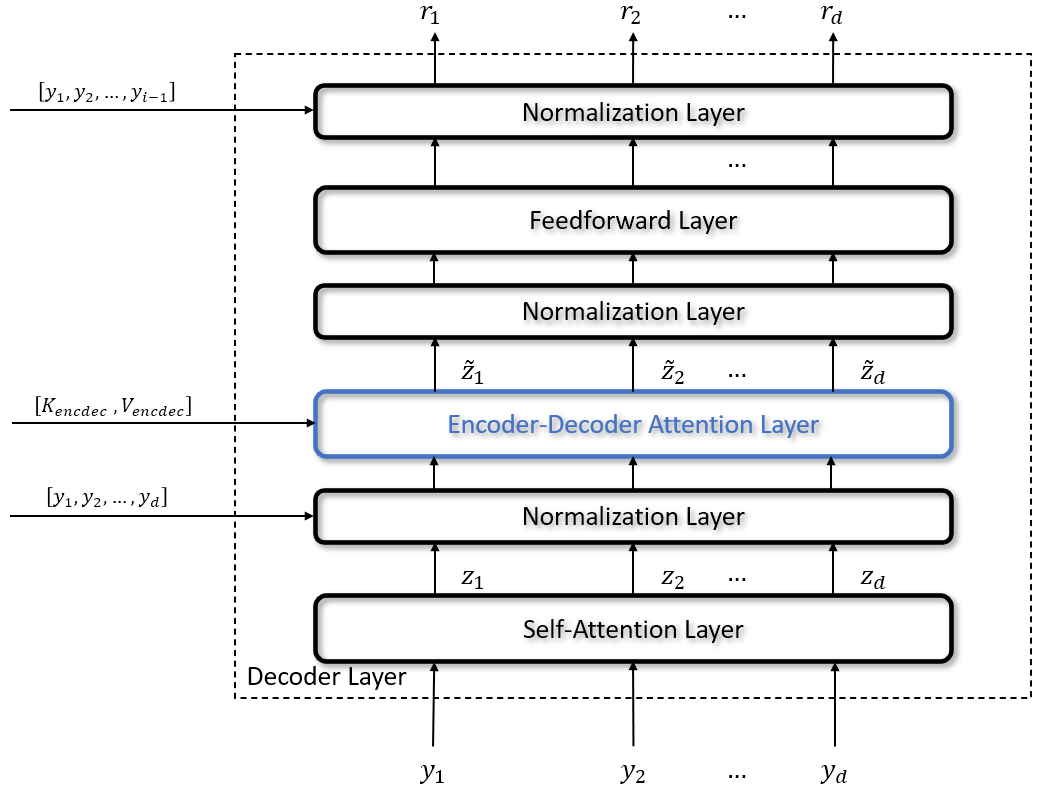
\includegraphics[width=15cm, keepaspectratio]{images/an/transformer_decoder.png}
                    \caption{High-level representation of a Transformer Decoder Layer model.}
                    \label{fig:an_transformer_decoder}
                \end{figure}
                
                At the end of each step, a Layer Normalization is used to normalize each intermediate output against each Decoder layer input. Figure \ref{fig:an_transformer_decoder} illustrates the architecture of one Decoder layer. \newline
                At the end, a combination of a Linear layer and a Softmax layer computes a probability distribution over all the possible next element of the output sequence $p_{dec}$, starting from the last result sequence $\mathbf{r_d}$. In the case of Neural Machine Translation, this final computation outputs the probability distribution over all the possible next words to be chosen, where the set of all possible words is called Vocabulary, which is fixed and decided before-hand. \newline
                The distribution $p_{dec}$ can be used both to train the network against the actual distribution, which will represent a dirac distribution on the correct next element of the output sequence of the dataset, and to predict the next element of the output sequence so to let the Decoder continue predicting other output elements.
                
        \subsection{Advantages over Recurrent Networks}
        \label{selfan:adv_recur}
            In their work, \pcite{an:transformer} highlight the advantages of the Transformer architecture against a "classic" Recurrent Sequence-to-sequence model. \newline
            The most significant improvement is found in the amount of computation that can be parallelized, which is one of the worst aspect of the Recurrent Sequence-to-sequence models. Infact, in order to coherently maintan their internal states, Recurrent models need to process each element of the input sequence sequentially, leaving little room to parallel computation. Instead, the Transformer can accept all elements of the input sequence at once and in practice it only needs key vector and value vectors to be ready for the score and attention computation for each element. Self-Attention computations and the Feedforward network computations for each element are not dependent on other elements of the sequence, except for key vectors and value vectors. This difference translates into Recurrent models requiring $O\left(e\right)$ sequential operations, where $e$ is the length of the input sequence, while the Transformer only needs $O(1)$, a constant amount of sequential operations. \newline
            Another significant improvement concerns the path length between long-range dependencies in the architecture, where the length is measured in term of sequential operations. Shorter path lengths allows for an easier understanding of the dependencies between any two elements of the input and output sequences, especially of the longer ones. In this regard, for the same reason as before, the Recurrent models requires to have a maximum path length between any two elements of the input and output sequence that is $O\left(e\right)$, while the Transformer maximum path length is still constant. \newline
            These advantages are supported by results provided by \pcite{an:transformer}, which shows how the Transformer is able to outperform other sequence-to-sequence models, also requiring lower computation costs for training the model.
    
    \newpage
    \section{Masked Autoregressive Flow}
        \label{prel:maf}
        % Introduction -> Why it's important & Autoregressive + Normalizing flows
        This section is dedicated to the presentation of Masked Autoregressive Flow (MAF), a density estimation technique based on neural networks proposed by \pcite{de:maf}, which stems from the combination of Neural Autoregressive Density Estimation (NADE) and Normalizing Flows. Its purpose is the estimation of a joint density $p(\mathbf{x})$, where $\mathbf{x}$ is a set of variables, from a set of given samples $\{ \mathbf{x}_n \}$. At first, NADE and Normalizing Flows are presented in Section \ref{subs:nade} and Section \ref{subs:norm_flows} respectively, since they are instrumental for the presentation of MAF, which is discussed in Section \ref{sub:maf}. \newline
        MAF has been adopted as a density estimation technique for the proposed network, thanks to its flexibility and ability to also estimate densities conditioned upon another set of variables $\mathbf{y}$. Infact, MAF constitutes the network through which the original network Module is optimized to drive its internal state towards the representation of a belief distribution of the current, yet unobserved, state of the environment. The specific details of the implementation are presented in Section \ref{ow:beliefmodule}.
        
        % Neural Autoregressive Density Estimation
        \subsection{Neural Autoregressive Density Estimation}
        \label{subs:nade}
            NADE is a density estimation technique presented by \pcite{de:nade}, which relies on the chain rule of probability in order to decompose a density $p(\mathbf{x})$ in the product of several mono-dimensional conditional densities as follows:
            
            \[ p(\mathbf{x}) = \prod_{i} p(x_i | \mathbf{x}_{-i} ) \]
            
            where $x_i$ represents i-th dimension in $\mathbf{x}$ and $\mathbf{x}_{-i}$ represents the subset of dimensions  $(x_j)_{j\in[1,\dots,i+1]}$. As a consequence, NADE is sensible to the order of the dimensions. In practice, each monodimensional density $p(x_i | \mathbf{x}_{-i} )$ is modeled as a parametric density, whose parameters are function of an internal state $h_i$. Thus, Recurrent networks such as LSTM or GRU can be deployed to recursively update the internal state $h_i$ while taking as input each single dimensions of $\mathbf{x}$.
            
            \subsubsection{Masked Autoencoder for Distribution Estimation}
                As it happens for Sequence-to-sequence models, relying on Recurrent mechanisms severely hinders parallel computation possibilities (see Section \ref{sota:selfan}). Infact, a Recurrent model for NADE would require to sequentially update its internal state a number of times equal to the number of variables contained in $\mathbf{x}$. In order to overcome this limitation, a fully-connected model can be exploited to receive all $x_i$ as input and producing the same amount of outputs at once, along with a mask that drop the connections of each variable $x_i$ with its "successors" in the variable order. The result of this approach is Masked Autoencoder for Distribution Estimation, presented by \pcite{de:made}, upon which MAF implementation is based.
                
        % Normalizing Flows
        \subsection{Normalizing Flows}
        \label{subs:norm_flows}
            Normalizing Flows is another kind of neural density estimator that relies on modeling density $p(\mathbf{x})$ as a base density $q(\mathbf{u})$ transformed through an invertible and differentiable function $f$:
            
            \begin{align}
                \mathbf{x} = f \left( \mathbf{u} \right) \label{eq:normflow}
            \end{align}
            Given $f$ and $q$, the target density $p(\mathbf{x})$ can be recovered as:
            
            \[ p(\mathbf{x}) = q(f^{-1}(\mathbf{x})) \abs*{ det \left( \frac{\partial f^{-1}}{\partial \mathbf{x}} \right) } \]
            
            Thus, for the implementation to be tractable the following requirements need to be met:
            \begin{itemize}
                \setlength\itemsep{0.05em}
                \item The base density $q$ needs to be easily evaluated from the computational point of view, which usually leads to the choice of a standard Gaussian distribution;
                \item The transformation function $f$ must be easily invertible and its Jacobian fast to compute.
            \end{itemize}
            At last, it is important to mention the following property: if two given  transformation functions $f_1$ and $f_2$ meet the aforementioned requirements, their composition $f \coloneqq f_1 \circ f_2$ still meets the requirements. This allows for stacking up different "layers" of transformation without compromising the overall tractability of the Normalizing flow, which is one of the property upon which MAF is based.
            
        % Masked Autoregressive Flows
        \subsection{Masked Autoregressive Flows}
        \label{sub:maf}
            As explained in the introduction to this section, MAF is a neural density estimator that is based on both NADE, more specifically MADE approach, and Normalizing Flows. Specifically, MAF relies on the chain rule of probability in order to split the target density $p(\mathbf{x})$ in several monodimensional conditional densities, each of which is then modeled as a Normalizing Flow.
            \\\\
            At first, each monodimensional conditional density is parameterized as a standard Gaussian density:
            \begin{align}
                p(x_i | \mathbf{x}_{-i} ) &= \mathcal{N} \left(x_i | \mu_i, (e^{\alpha_i})^2 \right)\label{eq:maf_gauss_1}\\
                \mu_i &\coloneqq f_{\mu_i}(\mathbf{x}_{-i})\nonumber\\
                \alpha_i &\coloneqq f_{\alpha_i}(\mathbf{x}_{-i})\nonumber
            \end{align}
            where $f_{\mu_i}$ and $f_{\alpha_i}$ are functions dedicated to compute respectively the mean and log standard deviation of the i-th variable in $\mathbf{x}$.
            \\\\
            It is possible to observe that, given a random variable $u_i$ sampled from $\mathcal{N}(0,1)$, each variable $x_i$ can also be expressed in the following way:
            \begin{align}
            \label{eq:maf_gauss_2}
                x_i = u_i e^{\alpha_i} + \mu_i
            \end{align}
            which represents the transformation function $f_i$  for each variable $x_i$. Each $f_i$ is easily invertible, given $x_i$ it is possible to retrieve the $u_i$ that generated it in Equation \ref{eq:maf_gauss_1} as follows:
            \begin{align}
                u_i = (x_i - \mu_i)e^{-\alpha_i}
            \end{align}
            At this point, the model can be represented using vectors to comprise the entire set of variables, retrieving a Normalizing Flow representation: $\mathbf{x} = f(\mathbf{u})$, where $\mathbf{u} = (u_1, u_2, ..., u_I)$ is the set of random variables that generated variables in $\mathbf{x}$, with $I$ being the total number of variables. Specifically, $\mathbf{u}$ is a random variable sampled from a Gaussian distribution $\mathcal{N}(\mathbf{0},\mathbf{I})$, where $\mathbf{0}$ is an $I \times I$ null matrix and $\mathbf{I}$ is the $I \times I$ identity matrix.
            \\\\
            At last, given the definition of $f$, its Jacobian is triangular by construction, which in turn means that it is easily retrieved as follows:
            \begin{align}
                \abs*{ det \left( \frac{\partial f^{-1}}{\partial \mathbf{x}} \right) } = e^{-\sum_{i}^{I} \alpha_i}
            \end{align}
            
            \subsubsection{Stacking Multiple Models}
                The flow described so far between $\mathbf{x}$ and $\mathbf{u}$ represents a single layer in the entire MAF architecture. Infact, MAF is based on stacking up several flows, each of which models the output of the previous flow and handle out variables to be modeled by the next flow. The possibility of stacking different models on one another is a key aspect of MAF architecture, since it provides it with powerful and precise density estimations: \pcite{de:maf} shows that their model is able to learn multimodal conditionals, even if MAF is only using unimodal conditionals. \newline
                In practice, each function $f = \{ f_{\mu_i}, f_{\alpha_i} \}$ is has a MADE structure: a fully connected model that accepts $I$ inputs in order to provide $I$ outputs, which is then masked by using a suitable binary matrix in order to zero out connections that would disrupt the autoregressive property. Specifically, the $i$-th input is only connected to previous ones. As previously explained, this particular technique allows for exploiting a more efficient parallel computation w.r.t. a recurrent implementation.
                
            \subsubsection{Conditional MAF}
                The autoregressive property makes MAF easy to be extended to conditional density estimation, the task of estimating the density $p(\mathbf{x}\vert\mathbf{y})$ given a set of examples $\{ \mathbf{x}_n, \mathbf{y}_n\}$, with $\mathbf{x} = (x_1, x_2, ..., x_I)$ and $\mathbf{y} = (y_1, y_2, ..., y_J)$. In practice, the vector $\mathbf{y}$ is simply appended to the conditional variables in each of the unimodal densities that follows the chain rule of probability:
                \begin{align}
                    p(\mathbf{x}\vert\mathbf{y}) = \prod_{i} p(x_i \vert \mathbf{x}_{-i}, \mathbf{y})
                \end{align}
                The approach of appending $\mathbf{y}$ carries over to the MADE implementation: each MAF layer takes as input the previous layer variables and $\mathbf{y}$ in addition. Since each variable $x_i$ is conditioned on the entire set of variables $y_j$, the binary mask will not drop their connections in each layer.
    
    
    \chapter{Original Work}
    \label{chp:ow}
    Finally, this Chapter is dedicated to the presentation and discussion of the original work and implementation of this research thesis. It is divided in four main sections. At first, Section \ref{ow:purposethesis} is concerned with the objective of the research, detailing a high-level model of the final proposed network and explaining which concepts, architectures and ideas have been borrowed from the State-of-the-Art research. Section \ref{ow:beliefmodule} presents the original module, called Belief-Estimation module, in all its components, mechanisms and design choices, by detailing step-by-step the operations that are involved and the loss function upon which it is. Afterwards, Section \ref{ow:deterministic_module} is concerned with the presentation of an intermediate step of our research, the State-Prediction module, which represents a simpler but meaningful network developed during the research that has been used as a baseline in Chapter \ref{chp:results}. At last, Section \ref{ow:application_sota} explains the range of applicability of the proposed Modules along with the actual implementation alongside a State-of-the-Art Reinforcement Learning algorithm, TRPO.
    
    \section{Original Implementation Objective}
    \label{ow:purposethesis}
        % Which of the State-of-the-Art topics have been used, when and why.
        %   - Delay Approaches: Model-Based Approach
        %   - POMDP Literature: Predictive-State Representation Approach
        %   - Deep Learning Literature: Attention Networks over Recurrent Networks
        As stated in the Introduction, the presence of delays does not represent a rare and particular case for MDP problems. Delays are present in the real world, they stem from many different sources, such as computational time or data transmission time, which are present exactly due to the physical implementation of the Agent. Thus, it is important to embed the presence of delays in the MDP framework, so to train agents that are capable to carry out a meaningful and precise decision-making process. However, literature specific to the DMDP framework is still scarce and wide-applicable solutions are yet to be found. \newline
        This thesis strive for the definition of a new implementation in the Model-Based approach for DMDP that is able to deal with both deterministic and stochastic delays in the context of both deterministic and stochastic environments. We would like to tackle the problem of delays with a heuristic approach: we provide to the RL algorithm a belief distribution of the current state in the form of a learnt vector representation.\newline
        Within this section, the design choices that lead to the definition of the Module's architecture are explained, detailing its structure in a step-by-step fashion in order to highlight how its design choices affected the final result. 
        
        \subsubsection{Assumptions of the Research}
            Before the presentation of the research development and results, it is important to highlight which assumptions and properties are taken. Throughout the rest of this chapter, the following statements and properties are assumed true:
            \begin{itemize}
                \setlength\itemsep{0.05em}
                \item Known delays: at each time-step, the Agent is aware of the amount of delay present, $d_t$, which is either constant or sampled from a stochastic process $d(t)$.
                \item Observation delays: we leverage the equivalency between observation delays and execution delays stated in Theorem \ref{th:dmdpred} by only referring to observation delays.
                \item Reward delays: reward delay is assumed equal to observation delay at each time-step, in order to avoid receiving information about an unobserved state.
                \item Time-Discretization: we assume that the amount of delay at each time-step is a multiple of the time-step unit of the environment. This is ensured through the simulation of the delay implemented. Further details are given in Section \ref{sub:simulated_delays}.
            \end{itemize}
            At last, we mention the fact that not all component of the module and the environments are originally implemented. The entire research is coded in Python 3.7 and we referred to known and trusted libraries such as PyTorch (\pcite{python:pytorch}) for network layers implementation and OpenAI Gym (\pcite{python:gym}) for environments implementation and OpenAI SpinningUp (\pcite{python:spinningup}) for RL algorithm implementation. The final implementation of modules and algorithms presented in this Chapter is available in this GitHub \href{https://github.com/Povaz/dmdp.git}{public repository}\footnote{Repository URL: \url{https://github.com/Povaz/dmdp.git}}.
            
        \subsection{Model-Based Approach}
            % Why Model-Based over Augmented and Memoryless
            In Section \ref{sota:delay_approaches}, three different approaches to the problem of delays are presented, each one with its own advantages and disadvantages. Among these three, Model-Based reveals to be the most flexible and applicable approach, giving room for experimenting different solutions for different environment and delay contexts. \newline
            The clear separation between the State Representation step and the Action Selection step, both presented in Section \ref{subs:modelbasedapproach}, allows for dividing the design process of a new architecture in the two correspondent tasks. Our implementation is focused on solving the State Representation step, while the Action Selection step is solved through an existing RL algorithm, TRPO in our case. Both other two approaches do not offer this freedom of design choice. \newline
            As explained in Sections \ref{subs:augmentedapproach} and \ref{subs:memorylessapproach}, Augmented State approach is characterized by an exponential State Space $\mathbf{I_d}$ and Memoryless approach requires ad-hoc solution to inject knowledge of delays. They both rely on the network structure of the RL algorithm, which in general does not support variable-size inputs, making unclear how to tackle stochastic delays. Model-Based approach addresses all these aspects within the State Representation step. \newline
            At last, the fact that the State Representation step has a specific observable objective makes it easier to evaluate the module's performances, since we do not need to always deploy a RL algorithm, train the whole architecture and inspect the Agent's final performances. Each design choice can be implemented and tested directly on the module by comparing its performances with previous iterations, inspecting their loss functions, for example. \newline
            For these reasons, the proposed new modules represent a new and original implementation of the State Representation step in the context of Model-Based approach for Delayed Reinforcement Learning problems. The Action Selection step is addressed by TRPO. Figure \ref{fig:module_modelbased_view} illustrates the entire architecture from the Model-Based approach point of view.
            \begin{figure}[!t]
                    \centering
                    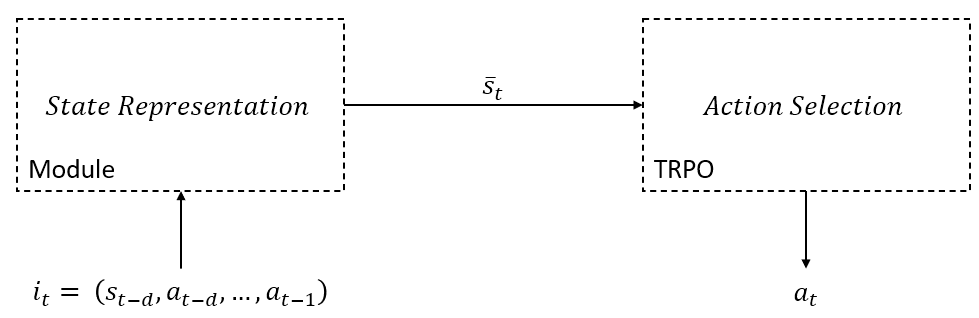
\includegraphics[width=15cm, keepaspectratio]{images/module/modelbased_view.png}
                    \caption{Model-Based approach view of the Modules architecture.}
                    \label{fig:module_modelbased_view}
            \end{figure}
            
        \subsection{Predictive-State Representation Approach}
            % What does the Module do in practice, which paradigms are applied
            Up until now, the original module has been pictured as a black box that implements the State Representation step in a Model-Based approach context. In order to further explain the details of the implementation, the main paradigm that leads the implementation must be defined. In this regard, POMDP literature have been useful to define the general approach. As explained in Section \ref{sota:pomdp}, DMDP framework is closely related to POMDP framework: DMDPs that are tackled with a Memoryless approach or by letting the Agent observe a belief can be formulated as a particular case of POMDP where the knowledge available to the Agent represents the observation perceived from the Environment. Predictive-State Representation (PSR) is a successful paradigm exploited by POMDP algorithms that is closely related to the Model-Based approach for DMDPs. For this reason, it has been adopted for guiding the practical implementation of the original modules.
            
            % - Learning a State Representation 
            \subsubsection{State Representation Learning}
                As presented in Section \ref{subs:psd}, Predictive-State Representation is applicable to architectures or networks that are able to maintain an internal state $h$ in addition to the usual output $y$, from processing their input. While $y$ is used by the Policy function to carry out action selection, the internal state $h$ is used to predict an observable quantity, $\bar{s}_t$. In addition to the usual performance measure $J$ that evaluates the Agent's decision-making process, a second loss function is defined to evaluate the ability of predicting $\bar{s}_t$, comparing it to the observed quantity, either the exact state $s_t$ or its belief distribution, for example. The observability of the said quantity is a key property, since its information needs to be available to the Agent at training time. The rest of this section is dedicated to a parallel comparison between the PSR architecture and the new developed modules, with the purpose of further detailing how they function.
                \\\\
                % - Takes as input available knowledge (observation/extended state)
                At each time-step $t$, PSR implementations take as input the current observation $o_t$, while our modules take as input the correspondent quantity in the context of the DMDP framework: the extended state $i_t$. In fact, both the current observation $o_t$ and the extended state $i_t$ represent the most updated information the Agent has available at each time-step. \newline
                % - Maintain an internal state h_t to predict future observation/states upon which a new Loss function is defined
                In both cases, the input is used to maintain the internal state $h$ by updating it through a mechanism implemented, denoted by a function $f$:
                \begin{align*}
                    h_t &= f_{PSR}(h_{t-1}, o_t)\\
                    h_t &= f_{Module}(h_{t-1}, i_t)
                \end{align*}
                where $f$ can be a Recurrent mechanism, implemented by means of LSTM or GRU network, or an Attention mechanism. In the POMDP case, the internal state $h_t$ is then used to predict the sequence of next observations $\mathbf{s_t} = (o_{t+1}, o_{t+2}, ..., o_{t+d})$ through another component of the network, called encoder in \pcite{pomdp:psd} or through $\theta_{pred}$ in \pcite{pomdp:rpsp}, for example. In our modules, the internal state $h_t$ is used to predict the sequence of yet unobserved states of the environment $\mathbf{s_t} = (s_{t-d+1}, s_{t-d+2}, ..., s_t)$ or their belief distributions. This representes the main advantage of our modules against their POMDP counterparts: since the information about the sequence of the exact states visited in the trajectory is available at training time, although delayed, it is possible to predict them or their distribution. In turn, this allows for defining a predictive loss function $L$ upon exact quantities, rather than partial observations, which is able to drive the modules towards a more meaningful internal state w.r.t. their POMDP counterparts. \newline
                % - Output the prediction (y/knowledgeaboutcurrentposition)
                At last, the output $y$ is produced from the internal state $h$. In the POMDP case, the internal state $h$ is directly provided to the Policy network $\pi$ as input. In the DMDP case, our modules can be designed to handle out to the Policy network $\pi$ a quantity that is most suitable given the properties of the environment: the current state prediction in deterministic environments or the internal state $h_t$, trained to represent the belief distribution of the current unknown state, in stochastic environments.
                
            % - MultiTask Learning Algorithm
            \subsubsection{Multi-Task Learning}
                The adoption of the PSR paradigm for the Modules also implies that, when coupled with a Reinforcement Algorithm, the entire network becomes an instance of Multi-Task Learning (MTL). In practice, the modules can also be used in a stand-alone fashion for the purpose of predicting current information, whether the exact state or a belief distribution, about the Agent unknown state $s_t$. \newline
                This also allows for highlight the main advantage of the modular approach: since the training is separated from the rest of the network, they can be considered as an interface between the extended state $i_t$ and the state representation $\bar{s}_t$. This process is invisible to the RL algorithm deployed and as a consequence any RL algorithm can be deployed. Hence the name of modules to denote the proposed networks. 
                %Figure \ref{fig:module_psr_view} illustrates the entire architecture from the Predictive State Representation point of view.
                
            % \begin{figure}[!t]
            %             \centering
            %             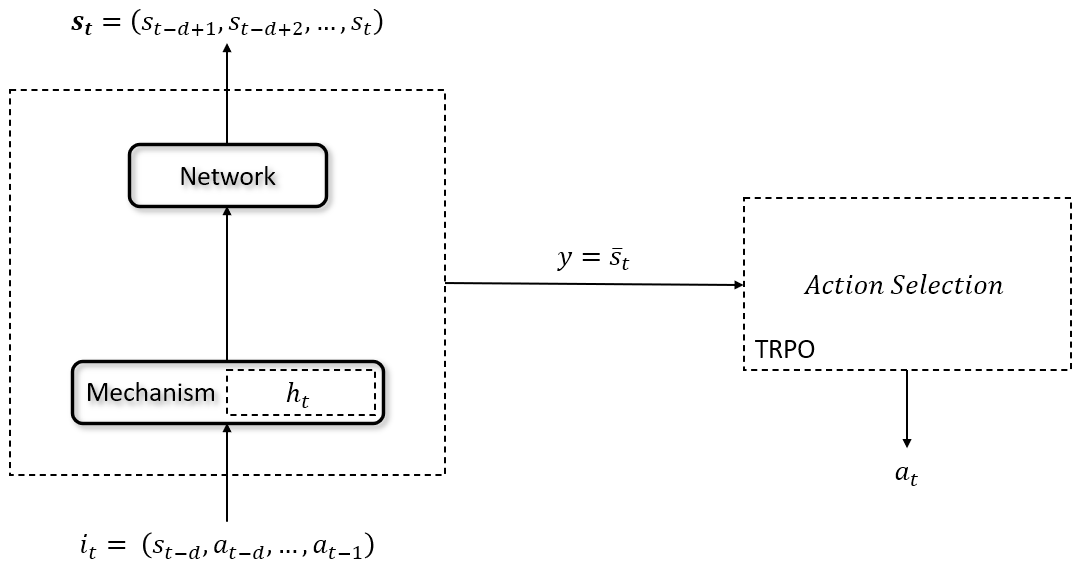
\includegraphics[width=15cm, keepaspectratio]{images/module/psr_view.png}
            %             \caption{Predictive-State Representation view of the Modules architecture.}
            %             \label{fig:module_psr_view}
            % \end{figure}
            
        \subsection{Self-Attention Mechanism}
            % - The modular property comes with a cost: computing the prediction for each extended state
            The modular property explained in the previous section is one of the strengths of the design of the Module. However, it also comes with the cost of passing each single extended state $i_t$ also through the module. This means that the computational overhead the Module introduces w.r.t. the Reinforcement Learning algorithm it is coupled with grows linearly with the total number of samples the entire network is trained upon. In the context of Reinforcement Learning, the total number of samples can easily reach millions, as shown in Chapter \ref{chp:results}. Thus, having an efficient mechanism that is able to maintain a meaningful internal state is a strong requirement. Otherwise, the risk is to lose the advantage introduced by the module because of the tremendous computational complexity the overall network requires. \newline
            
            % - Sequence-to-Sequence Models
            \subsubsection{Sequence-to-sequence Model}
                The modules' task can be seen as a translation from the extended state $i_t = (s_{t-d}, a_{t-d}, ..., a_{t-1})$ to the sequence of either unobserved states $(s_{t-d+1}, s_{t-d+2}, ..., s_t)$ or their belief distribution, which means that it is possible to model it through a Sequence-to-sequence model. In practice, this means that Recurrent and Attention mechanisms can be exploited to implement and mantain the internal state $h$, as explained in Section \ref{sota:selfan}. Attention is the chosen mechanism, given the optimization complexity that Recurrent implies: non-convex optimization and a number of sequential step that strictly depends on the length of the sequences involved, which in this case is dictated by the length of the delay.
            
            \begin{figure}[!t]
                    \centering
                    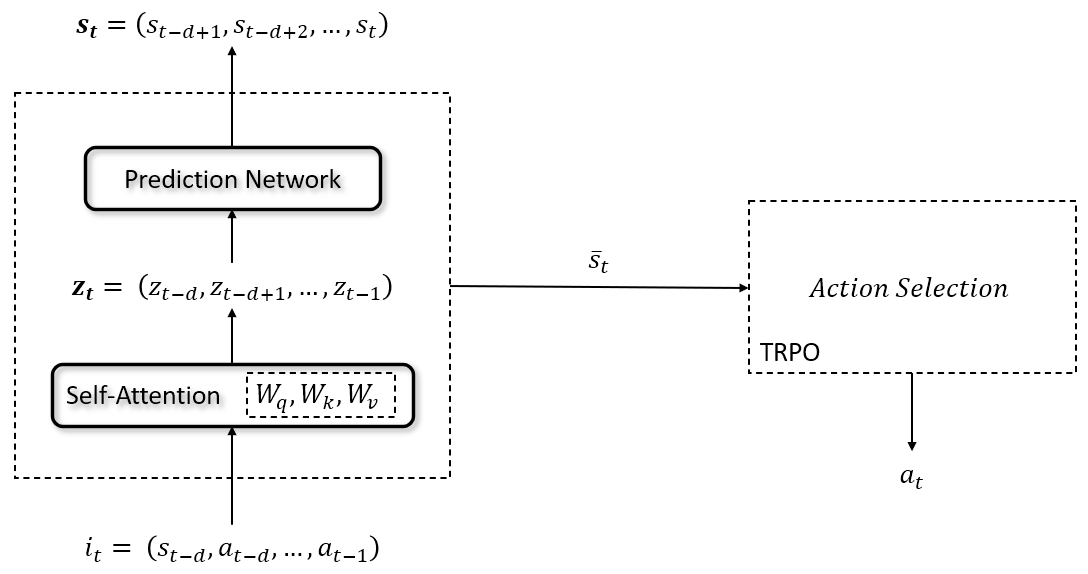
\includegraphics[width=15cm, keepaspectratio]{images/module/selfattention_view.png}
                    \caption{Self-Attention mechanism view of the Modules architecture.}
                    \label{fig:module_selfattention_view}
            \end{figure}
            
            % - Attention Mechanism provides a way to maintain a meaningful internal state, (W_q, W_k, W_v), also gives 
            \subsubsection{Self-Attention mechanism}
                In particular, Self-Attention provides a concrete implementation of the attention mechanism that is also free from Recurrent components while being able to compete with other state-of-the-art implementations, as illustrated in Section \ref{sub:transformer}. Thus the Modules' core components are represented by a sequence of Transformer's Encoder layers and a Prediction network. In practice, at each time-step $t$, the extended state $i_t$ is taken as input by the Self-Attention network, which produces the sequence of Attention vectors $\mathbf{z_t}$. Then, the Prediction network takes as input $\mathbf{z_t}$ and produces the state representation $\bar{s_t}$. The Prediction network remains generically defined at the moment because the two modules will present two different Prediction networks, which will be described in their correspondent Sections. Figure \ref{fig:module_selfattention_view} illustrates the entire architecture from the Self-Attention mechanism point of view.
                
    
    \newpage
    \section{Belief-Estimation Module}
        \label{ow:beliefmodule}
        % Introduction of the Belief-Estimation module
        In Section \ref{ow:purposethesis}, the overview of the module’s architecture is explained and illustrated. However, specific implementation details still need to be defined, along with the training and testing routine of the modules coupled with TRPO algorithm. \newline
        This section is dedicated to the Belief-Estimation module, designed to deal with stochastic environments, also supporting deterministic ones as a special case. Being able to cope with both deterministic and stochastic delays by construction, the Belief-Estimation module represents the final goal of this research thesis. In particular, we look for exploiting the Self-Attention mechanism provided by the Transformer's Encoders (Section \ref{sub:selfan}) to compute a fixed-length attention vector from a variable-length input sequence (Section \ref{sub:shape_input}), where the variability is present due to stochastic delays, which is then trained to represent the belief distribution of the current unobserved state through a MAF network (Section \ref{sub:maf_network}). At last, the belief representation is handled to a RL algorithm, TRPO in our case, in order to carry out action selection. The rest of the section is dedicated to present the sequence of components and operations that occur within them and to define the module's loss function.
        
        % Deterministic Module Structure:
        %   - From Extended State to (State, Action) couples (--> Words in NLT)
        \subsection{Shaping the Input}
            \label{sub:shape_input}
            The first issue encountered is the shape of the Module's input. Deciding to model the architecture as a Sequence-to-Sequence model means that the input shape must be a sequence, but the extended state $i_t = (s_{t-d}, a_{t-d}, ..., a_{t-1})$ does not immediately fit the needs. In fact, in Sequence-to-Sequence models each element of the sequence is an atomic element semantically equivalent to the others: in Neural Machine Translation, sequences are phrases and each element represents a word of the sequence, which are by definition equivalent to each other. In contrast, the extended state elements are not equivalent to each other: the first element is a state of the environment, while all the others are actions chosen by the Agent. In order to solve this issue, we decided to reshape the extended state in a sequence of couples $\mathbf{i_t}$ defined as follows:
            \[ i_t = (s_{t-d}, a_{t-d}, ..., a_{t-1}) \rightarrow \mathbf{i_t} =  \left[ (s_{t-d}, a_{t-d});  (s_{t-d}, a_{t-d+1}); ... ; (s_{t-d}, a_{t-1}) \right] \]
            Each couple $(s_{t-d}, a_{t-d+i})$ encapsulates the information of having observed state $s_{t-d}$ and decided to execute action $a_{t-d+i}$ a number of time-step $i$ later, with $0 \leq i \leq d - 1$. Also, reshaping makes each input element of the same size. This information is equivalent for each couple, exactly like words represents equivalent information in sentence.
            
        %   - Encoder (Transformer Architecture)
        \subsection{Self-Attention Network}
            \label{sub:selfan}
            After being reshaped into a sequence of couples, the input sequence is ready to be processed by the Self-Attention network. Similarly to the Transformer architecture, the main objective of this network is to produce a sequence of Attention vectors $\mathbf{z_t} = (z_{t-d}, z_{t-d+1}, ..., z_{t-1})$. Each Attention vector $z_{t-d+i}$, with $0 \leq i \leq d-1$, represents knowledge about the couple $(s_{t-d}, a_{t-d+i})$ and its correlation with the other couples according to the Self-Attention mechanism, explained in Section \ref{sub:transformer}. In fact, we believe that it is beneficial, if not crucial, to relate each couple to the others. In the undelayed MDP framework, each action selection is treated as independent from each other, thanks to the Markov Property (Property \ref{def:markov}). In the DMDP framework, this property does not hold for the sequence of actions chosen after the last observed state $s_{t-d}$. This means that looking only at the last observed states, thus considering each couple $(s_{t-d}, a_{t-d+i})$ independently from one another, is not sufficient to capture enough knowledge for a precise belief estimation.
            
            \subsubsection{Input Mapping}
        %       - Input Mapping (from Couples to intermediate representation --> Embedding in NLT)
                At first, each couple $(s_{t-d}, a_{t-d+i})$ of the input sequence $\mathbf{i_t}$ is translated through a Linear Input Mapping layer, which parameters needs to be learnt throughout the training process. In practice, each couple is treated as a vector and the following operation occurs in the Input Mapping layer:
                \[ x_{t-d+i} = ReLu \left( \theta_{input}^{T} * [s_{t-d}, a_{t-d+i}] + b_{input} \right)\]
                with $0 \leq i \leq d - 1$. The sequence of mapped couples is denoted by $\mathbf{x_t} = (x_{t-d}, x_{t-d+1}, $ $..., x_{t-1})$. This step of the process can be seen as an embedding of each couple, with the same conceptual meaning that Word Embedding holds in the case of Neural Machine Translation. Thus, the couples are translated from a vector of dimension $State Dimension + Action Dimension$ to a vector of dimension $enc_{dim}$, which represents an hyperparameter of the Module. At last, the result of the Input Mapping is passed through a ReLu activation function, which is so defined:
                \[ ReLu(x) = x^{+} = max(0, x) \]
                \noindent
                Optionally, we inserted the possibility to rescale the couples before the Input Mapping takes place. Each element of each couple $(s_{t-d}, a_{t-d+i})$ is normalized in the interval $[-1,1]$. We believe this option is necessary because the couples vectors $(s_{t-d}, a_{t-d+i})$ holds elements with very different physical meaning: $s_{t-d}$ represents the state dimensions while $a_{t-d+i}$ represents the action dimensions, which means that, in general, they may assume values of different order of magnitude. Thus, rescaling them to match the same interval $[-1,1]$ avoids implicitly assigning a greater importance to dimensions that holds the largest values, as it would happen otherwise, due to numerical operations within the network. Whether rescaling the couples or not is an hyperparameter of the Module.
                
            \subsubsection{Positional Encoding}
        %       - Positional Encoding (Position in the sequence matters)
                As explained in Section \ref{sub:transformer}, the Transfomer architecture allows for encoding positional information within each element of the input sequence. In fact, as it happens for words in a sentence, the order and position of each elements matters, since the sequence of actions in the original extended state $i_t$ represents the sequence of decisions made by the Agent. Following Equation \ref{eq:pos_enc}, a vector $p_i$ encoding positional information is computed and added to each element of the input sequence $x_{t-d+i}$:
                
                \[ x_{t-d+i}^{pos} = x_{t-d+i} + p_i \]
                \noindent
                In order to correctly implement Positional Encoding, the hyperparameter $enc_{dim}$, which defines $x_{t-d+i}$ dimension in the Input Mapping, must be equal to $p_i$ dimension. For simplicity of notation, $x_{t-d+i}^{pos}$ will still be denoted by $x_{t-d+i}$.
                
            \subsubsection{Layer Normalization}
        %       - Layer Normalization
                After the Positional Encoding is embedded in the sequence $\mathbf{x_t}$, a Layer Normalization is used to normalize values of each element $x_{t-d+i}$. Following Equation \ref{eq:layer_norm}, the following computation is carried out on each element $x_{t-d+i}$:
                
                \[ x^{norm}_{t-d+i} = \frac{x_{t-d+i} - \mathbf{E} \left[ x_{t-d+i} \right]}{\sqrt{\mathbf{Var} \left[ x_{t-d+i} \right] + \epsilon}} * \gamma + \beta\]
                
                where $\mathbf{E} \left[ x_{t-d+i} \right]$ and $\mathbf{Var} \left[ x_{t-d+i} \right]$ are estimated element-wise on the input batch the module is supplied with at each training process; $\epsilon$ represents a low value for numerical stability, usually set to $10^{-5}$, while $\gamma$ and $\beta$ represents learnable parameters of the layer and thus for the module. Again, for simplicity of notation, $x^{norm}_{t-d+i}$ will still be denoted as $x_{t-d+i}$.
                
            \subsubsection{Causal Mask}
        %       - Optional: Causal Mask (True for Deteministic in our results)
                Before processing the sequence $\mathbf{x_t}$ through the Encoder layers, we adopt the Input Sequence Mask option, presented in seciton \ref{sub:transformer}, in order to embed temporal causality within the model. Thus, we construct a Causal mask to be supplied to the Encoder Layer's implementation. A Causal mask is a mask that zeroes out all elements' score that come after the currently processed element, thus letting it relate only to previous elements. The idea behind the implementation of the causal mask is that each action in the extended state $i_t$, and thus each element in $\mathbf{x_t}$, is only affected by previous actions and not the following ones. Thus, avoiding to relate each element $x_{t-d+i}$ with the future ones represents an optimization of the module learning process: while we expect the module could reach the same performances, it would require a higher number of parameters, possibly hindering the training process, by not applying a Casual mask. Whether applying the Causal mask or not is an hyperparameter of the Module.
                
            \subsubsection{Encoder Layers}
            %   - Encoder Layers
                After Normalization Layer, a Transformer Encoder is implemented in order to carry out the Attention mechanism in the Module. As explained in Section \ref{sub:transformer}, the Transformer Encoder stacks one or more Encoder layers sequentially. Each one of them takes as input either the sequence $\mathbf{x_t}$ or their previous layer' output sequence $\mathbf{z_{t}^{j}}$, where $j$ denotes the outputs of the $j$-th Encoder layer along with the Causal mask, if it is enabled for the module. Encoder layer's attention computation is not modified from the Transformer's original implementation. However, our Module is based on the PyTorch implementation of a Transformer Encoder layer and the precise details of its implementation can be found in PyTorch documentation. \newline
                The result obtained is the sequence of Attention vectors, $\mathbf{z_t} = (z_{t-d}, z_{t-d+1}, ..., z_{t-1})$, where each element contains the information regarding the correspondent $x_{t-d+i}$ element and its attention relation with other elements of $\mathbf{x_t}$. The number of Encoder layers $e$, the dimension of the encoder vectors $q$, $k$ and $v$, denoted as $enc_{dim}$ and the dimensions of the Feedforward layers $enc_{ff}$ represent hyperparameters of the Module.
                
            \subsubsection{Encoder Output Mapping}
            %   - Encoder Output Mapping (from Encoder Layers Dimension to Attention Vectors Dimension)
                The last step of the Self-Attention network is a Linear Output Mapping, which serves the purpose to match Attention vectors dimension $enc_{dim}$ to the dimension expected by the Prediction network, $pred_{dim}$. The computation is analogous to the Linear Input Mapping, for each element in the sequence $\mathbf{z_t}$:
                \[ z^{pred}_{t-d+i} = ReLu \left( \theta_{output}^{T} * z_{t-d+i} + b_{output} \right)\]
                where $\theta_{output}$ and $b_{output}$ represents learnable parameters and the dimension $pred_{dim}$ a hyperparameter of the State-Prediction Module. As done previously, the elements $z^{pred}_{t-d+i}$ will still be denoted as $z_{t-d+i}$ for simplicity of notation.
        
        % MAF Implementation as Prediction Network
        \subsection{Masked Autoregressive Flow Network}
            \label{sub:maf_network}
            As explained in Section \ref{prel:maf}, Masked Autoregressive Flow is a neural density estimation technique: it allows for estimating a conditional density $p(\mathbf{x}\vert\mathbf{y})$ given a set of examples $\{\mathbf{x}_n, \mathbf{y}_n \}$, where $n$ represents the number of total examples. Our objective is to use MAF network to estimate the density of the unobserved states $s_{t-d+i}$ conditioned on the extended state $i_t = (s_{t-d}, a_{t-d}, ..., a_{t-1})$, thus $p(s_{t-d+i} \vert i_t)$ with $1 \leq i \leq d$.
            \\\\
            In order to achieve our objective, we need to represent the learnt density $p_{pred}$ as a transformation by an invertible and differentiable function $f_{pred}$ of a base Gaussian density $q$. In practice, $f_{pred}$ is composed by a number of function couples $(f_{\mu_j}, f_{\alpha_j})$ equal to the state dimensions, denoted as $sdim$, since each couple is specifically tasked to build each dimension of the unobserved state $s_{t-d+i}$ as follows:
            
            \begin{align}
                s_{t-d+i}^{j} &= u_j e^{\alpha_j} + \mu_j\label{eq:beliefmod_normflow}\\
                \mu_j &\coloneqq f_{\mu_j} (\mathbf{u_{-j}}, z_{t-d+(i-1)})\nonumber\\
                \alpha_j &\coloneqq f_{\alpha_j}(\mathbf{u_{-j}}, z_{t-d+(i-1)})\nonumber
            \end{align}
           
            where $\mathbf{u} = (u_1, u_2, ..., u_{sdim}) \sim q$, its elements are denoted as $u_j$ and the subscript $-j$ denotes all elements in $\mathbf{u}$ before the $j$-th; $z_{t-d+(i-1)}$ is the Attention vector produced by the Self-Attention network correspondend to the state $s_{t-d+i}$, note that the additional -$1$ in the subscript is used to align the sequence of Attention vector $\mathbf{z_t}$ to the sequence of unobserved states. At last, the function couples $(f_{\mu_j}, f_{\alpha_j})$ are parametric functions, which parameters represents the set of learnable parameters of the MAF network. To be more specific w.r.t. the MAF original implementation, the set of equation and definitions \ref{eq:beliefmod_normflow} correspondes directly to the set of equations and definitions \ref{eq:maf_gauss_1} and \ref{eq:maf_gauss_2}. \newline
            In practice, we are conditioning density $p_{pred}$ by appending the Attention vectors $z_{t-d+(i-1)}$ produced by the Self-Attention network to the samples $\mathbf{u_{-j}}$ from the base density $q$, as explained in Section \ref{sub:maf}. This allows for expressing $p_{pred}$ through the following representation:
            \begin{align}
                \label{eq:beliefmod_ppred}
                p_{pred} (s_{t-d+i} \vert z_{t-d+(i-1)}) = q \left( f_{pred}^{-1} \left(s_{t-d+i}, z_{t-d+(i-1)} \right) \right) \abs*{det \left( \frac{\partial f_{pred}^{-1}}{\partial s_{t-d+i}} \right)}
            \end{align}
            which is a direct application of Equation \ref{eq:normflow}. Given the recursive nature of the network, which produces each state dimension at each recursion, the right-hand side determinant is easily computed, because $f_{pred}$'s Jacobian is a triangular matrix.
            
            % Explain how the Module is optimized --> Loss Function and Gradient-Based
            \subsubsection{Loss Function}
            Up to this point, we have explained how it is possible to compute the estimated density $p_{pred}$. To quickly recap, each extended state $i_t = (s_{t-d}, a_{t-d}, ..., a_{t-1})$ is first reshaped into couples $(s_{t-d}, a_{t-d+i})$ with $0 \leq i \leq d-1$. Each couple is then processed throughout the Self-Attention network, which produces the sequence of attention vectors $\mathbf{z_t} = (z_{t-d}, z_{t-d+1}, ..., z_{t-1})$. Each attention vector $z_{t-d+(i-1)}$ is then used with its correspondent unobserved state $s_{t-d+i}$, with $1 \leq i \leq d$, to compute the conditional density $p_{pred} (s_{t-d+i} \vert z_{t-d+(i-1)})$ through Equation \ref{eq:beliefmod_ppred}. \newline
            Then Belief-Estimation module is trained upon the following loss function $L_{belief}$: 
            
            \begin{align}
                L_{belief}(\mathbf{z_{t}}, \mathbf{s_t}) \coloneqq \sum_{i}^{d} D_{KL} \left( p(s_{t-d+i} \vert i_t) || p_{pred}(s_{t-d+i} \vert z_{t-d+(i-1)}) \right)
            \end{align}
            
            where $\mathbf{s_t}$ is the sequence of unobserved states related to the extended state $i_t$ and $D_{KL}$ represents the Kullback-Leibler divergence. A replay buffer is implemented to retrieve a set of samples to compute $L_{belief}$, details are given in Section \ref{sub:dtrpo_buffers}. In practice, $L_{belief}$ computes the distance between the true state distribution conditioned on the extended state $i_t$ and the predicted state distribution conditioned on the attention vectors $\mathbf{z_t}$. The idea behind this design decision is that we would like to enforce the attention vectors to comprise all the available knowledge about the Agent's current, but unobserved, position by driving it towards a finite vector representation of the current belief distribution which is then handled out to the RL algorithm, as a State Representation according to the Model-based approach. Hence the name of the module: Belief-Estimation module. \newline
            For the actual implementation, $L_{belief}$ is substituted by using the following log-likelihood approximation:
            
            \begin{align}
                L_{belief}(\mathbf{z_t}, \mathbf{s_t}) \coloneqq \sum_{i=1}^{d} \log p_{pred} \left(s_{t-d+i} \vert z_{t-d+(i-1)} \right)
            \end{align}
            \noindent
            By construction, $p_{pred}$ is differentiable w.r.t. its set of learnable parameters, thus we can exploit any gradient-based optimization algorithm to optimize the entire network. We decided to exploit ADAM, an algorithm for first-order gradient-based optimization proposed by \pcite{opt:adam}, to optimize the module. In practice, we exploited two different instances of ADAM algorithm: the first optimizes the MAF network parameters, backpropagating until the conditional $\mathbf{z_t}$, while the second optimizes the Self-Attention network, backpropagating from $\mathbf{z_t}$ to the start of the module.
        
    \newpage
    \section{State-Prediction Module}
    \label{ow:deterministic_module}
        During the development of the research, we focused first on deterministic environments given their reduced complexity w.r.t. stochastic environments, in order to test our approach. Thus, before the complete definition of the Belief-Estimation module was reached, we developed an intermediate result, designed to solve the delay problem in deterministic environments: the State-Prediction module. Its structure is similar to the final design, in fact it exploits the same input shaping process (Section \ref{sub:shape_input}) and Self-Attention network (Section \ref{sub:selfan}). However, instead of providing a belief estimation through a MAF network, it provides a direct prediction of the current, unobserved Agent's position through a Linear layer. The entire network is trained upon a mean-squared error loss, or L2 loss, computed between the state prediction $\tilde{s}_t$ and the observed delayed state $s_t$. The state prediction is then handled out to the RL algorithm. This section is dedicated to detailing the Prediction network.
        
        \subsection{Prediction Network}
        \label{sub:pred_network}
        %   - Output Mapping (from Attention Vectors to Predicted States)
            As introduced, the last step of the State-Prediction Module is concerned with deriving the sequence of state prediction $\mathbf{s_t}$ from the sequence of Attention vectors $\mathbf{z_t}$. A Linear layer is implemented for the task and the computation is analogous to the one previously presented:
            
            \[ \tilde{s}_{t-d+i+1} = ReLu \left( \theta_{pred}^{T} * z_{t-d+i} + b_{pred} \right)\]
            
            where $\theta_{pred}$ and $b_{pred}$ are learnable parameter for the Module. Note that the dimension of the output vectors $\tilde{s}_{t-d+i+1}$ is not a parameter, since it is the state dimension, dictated by the Environment. We denote by $\mathbf{\tilde{s}_t} = (\tilde{s}_{t-d+1}, \tilde{s}_{t-d+2}, ..., \tilde{s}_t)$ the output sequence of the State-Prediction module. 
            \\\\
            At last, it is important to specify that in the case of rescaling the input during the Input Mapping explained in the previous section, the output could be rescaled back to match the actual state dimensions values, by multiplying each dimension for the scaling factor used at the beginning. 
            
            % Explain how the Module is optimized --> Loss Function and Gradient-Based
            \subsubsection{Loss Function}
                Now that the output sequence of the module has been defined, it is also possible to specify how the State Prediction module is optimized. We define a mean-squared error loss function, denoted as $L_{pred}$, over the output sequence $\mathbf{\tilde{s}_t}$ and the sequence of actually, delayed observed states $\mathbf{s_t} = (s_{t-d+1}, s_{t-d+2}, ..., s_t)$:
                \begin{align}
                    L_{pred} (\mathbf{\tilde{s}_t}, \mathbf{s_t}) \coloneqq \frac{1}{d} \sum_{i}^{d} \left( s_{t-d+i} - \tilde{s}_{t-d+i}\right)^{2}
                \end{align}
                after which any gradient based optimization algorithm can be exploited to update the module's parameters, since by construction the State-Prediction module is differentiable w.r.t. its set of learnable parameters. As for the Belief-Estimation module, we exploit the ADAM optimization algorithm to optimize the module. A replay buffer is implemented to retrieve a set of samples to compute $L_{pred}$, details are given in Section \ref{sub:dtrpo_buffers}. In practice, by optimizing the State-Prediction module using $L_{pred}$, we drive the entire network towards the prediction of the current, unobserved state, which is handled out to the RL algorithm as a State Representation according to the Model-based approach. Hence the name of the module: State-Prediction Module.
                
    \newpage
    \section{Applications with State of the Art Algorithms}
    \label{ow:application_sota}
        % Introduction:
        %   - Seq2Seq usually trained in ML context (data set)...
        %   - ...we needed a RL context (trajectories)
        %   - Thus Module trained along with Policies/Values
        %   - Thus a Prediction Buffer 
        In the previous sections, both modules have been presented along with their loss functions, which they are trained upon. At this point, it is important to define the details about its deployment: how we sample the environment to populate the buffer and the module interaction with the RL algorithm. In this section, we first describe the functioning of the buffers (Section \ref{sub:dtrpo_buffers}) and then we detail the implemented application alongside TRPO algorithm (Section \ref{sub:dtrpo}). The implementation of the new algorithms can be found in the following GitHub public repository: 
        
        % Training Loop in RL + Prediction Buffers
        \subsection{Training and Prediction Buffers}
        \label{sub:dtrpo_buffers}
            The main issue in designing the training procedure is concerned with the fact that, usually, Sequence-to-sequence models training is based on a fixed dataset of examples the model is trained upon, while RL algorithms rely on drawing a certain number of new trajectories at each epoch, which are then used to update its policy and value functions. Given the policy and value function updates, the distribution of the trajectories $p_{\tau}$ is not stationary through the epochs and it may change considerably: the final purpose is to retrieve an optimal policy, which will draw trajectories that are very different from the initial, randomly initialized, policy.
            The fact that the trajectory distribution $p_{\tau}$ is not stationary during training poses serious constraints on the training procedure:
            \begin{itemize}
                \setlength\itemsep{0.05em}
                \item Supervised Learning approach: While it is feasible to gather an unlimited number of trajectories before training policy and value function, thus building a dataset of state representation $\bar{s}_t$, computed from the extended states observed, and correspondent unobserved states $s_t$, the policy function that would draw them is necessarily a poor randomly initialized one. Thus, in general, the policy would not be able to properly explore the environment and the built dataset cannot be considered reliable. In practice, we expect the module's performances to decrease whenever the policy starts drawing trajectories that visits new extended states w.r.t. the ones used to build the datasets. Furthermore, we should also consider the fact that building a better dataset from the environment implies gathering more samples from the environment. The time spent on building this dataset is directly subtracted from the time spent on training the policy, thus potentially reducing the overall final performances.
                \item Reinforcement Learning approach: At the same time, training the module upon the state representations $\bar{s}_t$ resulting from set of extended states visited at each epoch can be a limiting factor. The module would learn upon a different trajectory distribution at each epoch, thus potentially creating instability during the module's updates. In turn, the policy would be affected by a low quality state or belief representations as input.
            \end{itemize}
            \noindent
            In order to design a robust training algorithm for the modules, we need to find a middle-ground between this two extremes approaches.
            
            \subsubsection{Prediction Buffer}
                We decided to implement a Replay Buffer for the module, called Prediction Buffer, in order to bridge the gap between Reinforcement Learning and Supervised Learning. The introduction of a Replay Buffer has been proven to be very beneficial for the overall training process by \pcite{dql}.
                The Prediction Buffer allows for storing experienced trajectories: at each time-step $t$, the current extended state $i_t$ and the state contained in it, $s_{t-d}$ are stored in the Prediction Buffer. Due to delay presence, the two stored vectors are disaligned time-wise: the currently observed extended state $i_t$ is used to produce the sequence $(\bar{s}_{t-d+1}, \bar{s}_{t-d+2}, ..., \bar{s}_t)$, but provides the exact visited state $s_{t-d}$, which refers to $\bar{s}_{t-d}$. Since $\bar{s}_{t-d}$ has been produced by the previous $d$ extended states $(i_{t-d}, i_{t-d+1}, ..., i_{t-1})$, $s_{t-d}$ is actually used for each one them. Thus, the Prediction Buffer implementation needs to be able to handle the re-alignment between them. At the end of each epoch, the Prediction Buffer is sampled: the sequence of extended states selected are used to produce their correspondent sequences of state or belief predictions $(\bar{s}_{t-d+1}, \bar{s}_{t-d+2}, ..., \bar{s}_t)$ and along with the sequence of selected visited states $(s_{t-d+1}, s_{t-d+2}, ..., s_t)$ they are used to compute the loss function.
                \\\\
                Due to the re-alignment procedure, two different Prediction Buffers are implemented. The first is tasked with handling deterministic delays, which presents a fixed-length disalignment between $i_t$ and $s_{t-d}$, and it is denoted as Deterministic Prediction Buffer. The second is developed to specifically handle the presence of stochastic delays, hence denoted as Stochastic Prediction Buffer. As explained in Section \ref{sub:dmdp_stochdelays}, the presence of stochastic delays creates a complex interaction between the Agent and the environment, where the time disalignment between $\bar{s}_t$ and $s_t$ is not fixed and the sequence of experienced states may not follow the same order of the visited states. Thus, a separate implementation have been developed to specifically handle this situations. Thanks to the known delays assumption, both Prediction Buffer are aware of the amount of delay at each time-step, which makes the re-alignment task feasible.
                \\\\
                Prediction Buffers are characterized by their size, i.e. the number of samples it can contain, and by their batch size, i.e. the number of samples that are used to train the module at the end of each epoch. Whenever the Prediction Buffer is full, older samples are removed in favor of the newer ones. Both size and batch size are considered hyperparameters of the module, given their impact in the learning process. As a result, the module is trained with experience replay, learning upon both new and old samples in order to smooth the trajectory distribution changes throughout the epochs with the purpose of stabilizing the training process, overcoming the two critical issue described above.
                
        \subsection{Delay Trust Region Policy Optimization}
        \label{sub:dtrpo}
            
            % Better Explain the interaction between Modules and TRPO
            We decided to deploy both modules alongside TRPO algorithm, defining two variants of the same algorithm. We refer to the State-Prediction module deployment as L2-TRPO, given the nature of its loss function, while the Belief-Estimation module deployment has been called Delay TRPO or D-TRPO, in light of the fact that it represents our goal implementation. In practice, the modules presence is invisible to TRPO, which action selection is carried out unaltered from the original implementation upon a state space provided by the module. Thus, policy and value functions updates are implemented following Algorithm \ref{algo:trpo} specifications. Algorithm \ref{algo:dtrpo_l2trpo} illustrates both L2-TRPO and D-TRPO complete training algorithm: the differences between the two algorithms are contained within the module update and its Prediction Buffer routine. At last, we present the options implemented within L2-TRPO and D-TRPO designed to optimize the training procedure of the algorithms.
            
            \subsubsection{Pre-train Epochs}
            %   - Pretrain option for the Module
                Given the fact that all networks are randomly initialized at the start of the training process, the first epochs of training are characterized by low quality state or belief representation, which distribution is rapidly changing due to the gradient-based optimization method. As a consequence, policy and value networks updates during this first part of the training process are based on low quality information about the current position of the Agent in the environment, regardless of the type of module used and amount of delay present: the direction of optimization taken by their parameter vectors is not well-defined until the module is able to produce a better quality predictions. \newline
                In order to avoid wasting computational time and potentially lower the training quality of policy and value function, we believe it is useful to also have a way to decide to pre-train the module for a certain number of epochs before starting the Agent's training. We call this epochs Pre-train epochs and we consider the amount of pre-train epoch a hyperparameters of the algorithm, to be decided along the usual total number of training epochs. This allows for policy and value functions to be trained already upon meaningful state or belief representations.
                
            \subsubsection{Stopping the Module Training}
            %   - Stoptrain option for the Module
                On the other hand, it may be possible that the module is able to learn meaningful state or belief representation before the end of the whole training process. If this happens, continuing to update the module would be a waste of time and computational resources, which could be re-directed towards the policy and value function networks: the same time spent updating the module could be instead used to update TRPO for longer. At the same time, given the fact that the module is not updated anymore, its belief representation does not change over time. Distribution changes in the input for the policy and value networks can be a source of instability in the learning process, which is avoided during this last epochs of training, resulting in more robust updates. \newline
                For this reason, we inserted the possibility to choose at which epoch the module's training is stopped, which is considered a hyperparameter of the trianing algorithm and it needs to be decided along with the total number of epochs and the number of pretrain epochs.
                
                \begin{algorithm}[t]
                    \SetAlgoLined
                    \DontPrintSemicolon
                    \KwResult{Trained Policy $\pi_{\theta^*}$, Trained Module $mod_{\varepsilon^*}$}
                    Initialize module $mod$ parameters, $\varepsilon_0$ randomly and its hyperparameters\;
                    Initialize policy $\pi$ parameters, $\theta_0$\;
                    Initialize value function $v$ parameters, $\phi_0$\;
                    Initialize Prediction Buffer $size$ and $batch$\;
                    Initialize TRPO hyperparameters\;
                    Initialize number of training epochs $E$, the number of pre-train epochs $P_e$ and the stop epoch $S_e$, such that $P_e \leq S_e$\;
                    Set the maximum number of steps of each epoch $T$\;
                    \While{$e \leq E$}{
                        Set current time-step $t=0$\;
                        Initialize the environment, retrieving the first extended state, $i_0$\;
                        \While{$t \leq T$}{
                            Compute the current State/Belief Representation $\bar{s}_t = mod_{\varepsilon}(i_t)$\;
                            Select action $a_t = \pi_{\theta} (\bar{s}_t)$\;
                            Observe the next extended state $i_{t+1}$\;
                            Receive the reward signal $r_t$\;
                            Store current information in the Prediction Buffer:\;
                            \ \ \ \ \ Extract $s_{t-d}$ from extended state $i_t$\;
                            \ \ \ \ \ Store $s_{t-d}$ and $i_t$\;
                            \ \ \ \ \ Align $s_{t-d}$ with $(i_{t-d}, i_{t-d+1}, ..., i_{t-1})$\;
                            Update time-step $t=t+1$\;
                            \If{Episode is terminated}{
                                Initialize the environment, retrieving the first extended state, $i_{t+2}$\;
                                Update time-step $t=t+1$\;
                            }
                        }
                        \If{$e \leq S_e$}{
                            Update module $mod$ parameters, $\varepsilon_e$:\;
                            \ \ \ \ \ Sample the Prediction Buffer: $\{s_t, i_t\}_{batch}$\;
                            \ \ \ \ \ Compute $\bar{s}_t$ for each $i_t$: $\{s_t, \bar{s}_t\}_{batch}$\;
                            \ \ \ \ \ Compute the Loss Function $L_{pred}$/$L_{belief}$ using $\{s_t, \bar{s}_t \}_{batch}$\;
                            \ \ \ \ \ Optimize the module via ADAM algorithm\;
                        }
                        \If{$e \geq P_e$}{
                            Update policy $\pi$ parameters, $\theta_e$, via TRPO algorithm\;
                            Update value function $v$ parameters, $\phi_e$, via TRPO algorithm\;
                        }
                    }
                    \caption{D-TRPO and L2-TRPO Training Algorithms.}
                    \label{algo:dtrpo_l2trpo}
                \end{algorithm}
        
    \chapter{Results}
\label{chp:results}
    % Introduction
    This chapter is dedicated to the experiments done and results collected by training and testing the original proposed implementations along with a series of baseline algorithms. Section \ref{results:context} is concerned with presenting all the information regarding the context of the experiments, the simulated delay implementations and baseline algorithms choices. Section \ref{results:module_tuning} presents the process of parameters tuning for the modules' parameters and explains the roles and importance of each parameter in terms of concepts and performances. At last, within Sections \ref{results:deterministic} and \ref{results:stochastic} L2-TRPO and D-TRPO performances are evaluated and compared against the chosen baselines, drawing the conclusions about the original implementations' capabilities. All results and plots presented in this Chapter are also available in this GitHub \href{https://github.com/Povaz/dmdp.git}{public repository}\footnote{Repository URL: \url{https://github.com/Povaz/dmdp.git}}.
    
    \section{Experiments Context}
    \label{results:context}
    % Section dedicated to present the context of all tests/results
        Before diving into the experiments, it is important to establish the set of rules that have been followed during the whole process. At first, we will define how the environment tested works and which are its difficulties. Then, the delay implementation will be discussed: the presence of delay is simulated upon the environment, for both deterministic and stochastic delays. At last, the baseline algorithms used for comparison are presented and the choice motivations explained with them. All the assumptions and details exposed here will hold for the rest of the chapter, unless specified.
        
        \subsection{Inverted Pendulum}
        % Dedicated to explain how Inverted Pendulum works
            \begin{figure}[!b]
                        \centering
                        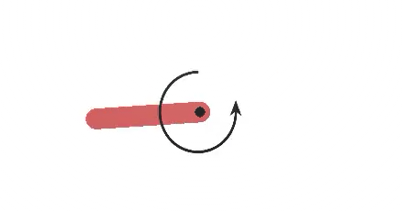
\includegraphics[width=13cm, keepaspectratio]{images/results/pendulum.png}
                        \caption{A representation of the Inverted Pendulum environment. The arc arrow represents the torque applied by the Agent.}
                        \label{fig:results_pendulum}
            \end{figure}
            The chosen environment is Inverted Pendulum. In this environment, a pole is hooked up to a fixed torque at one of its extremities and it is able to rotate using the torque as center of the rotation, describing a full circle. Gravity is applied to the pole at any istant, thus in absence of other forces the pole is drawn to the down-vertical position, at $\frac{3}{2}\pi$. At each time-step, the Agent is able to express a torque force to the pole, allowing it to swing around its rotation center, with the goal of bringing it to the up-vertical position, at $\frac{1}{2}\pi$. \newline
            At each time-step $t$, the state of the environment $s_t$ is represented by a 3-dimensional vector containing the cosine of the pole, the sin of the pole angle and its angular velocity. The Agent is able to express the torque force by controlling a scalar continuous action $a_t$, which values ranges between $-2$ and $2$. Negative action values indicates a torque in the opposite rotation direction. The Agent also receives a negative reward signal $r_t$ which is computed as a function of both pole position and the absolute value of the action chosen by the Agent, in such a way that position distant to up-vertical and higher intensity actions are penalized. Thus, the Agent objective is to swing the pole to bring it to the up-vertical position with a low intensity action, which in turn can be translated in the ability to reach the unstable equilibrium of the up-vertical position and mantain it. The Inverted Pendulum implementation has been provided by the Python OpenAI Gym Library and it has been used without any modifications. \newline
           There are two the main reasons for chosing this environment. The first is concerned with the precision of action selections it requires: the goal position is an unstable equilibrium, thus the agent not only must understand how to apply the torque to reach the position, but it also needs to be precised enough to maintain it until the end of the episode. Slight errors in the action selection may bring the pole down lowering the Agent performances significantly and the presence of delay is enhancing this property. The second reason resolves on the fact that the Agent is able to observe states that are composed by sin and cosine values, resulting from the same angle: the module needs to be able to output sufficiently precise state or belief representation to identify the Agent position, if not so, a given predicted state may not even be part of the State Space of the environment, hindering the policy learning process.
            
        \subsection{Simulated Delay Implementation}
        \label{sub:simulated_delays}
        % Dedicated to explain the Delay implementation
        %   - Deterministic Delay
        %   - Stochastic Delay
            As explained in Chapter \ref{chp:ow}, the presence of delays is simulated upon the environment. In practice, a wrapper is implemented around the environment and, at each-time step, it samples the amount of delay $d_t$, or simply $d$ in the case of deterministic delays, and manages the construction of the current extended state $i_t$ as well as the computation of the delayed reward signal $r_t$. Furthermore, it also manages the initialization of the environment: with the presence of delay, the Agent cannot have immediate access to the extended state at the first time-step of the episode, due to the fact that first state is not yet observed. Thus, we need to simulate the first $d$ steps by selecting $d$ random actions, until the first state is observed and the first extended state can be built unifying it to the sequence of actions. During this process, the delay is always assumed a integer multiple of the single time-step.
            
            \subsubsection{Deterministic Delays}
                Deterministic delays implementation is straightforward. The delay wrapper initialize the environment by selecting $d$ random actions for $d$ time-steps, storing the sequence of $d$ states $(s_0, s_1, ..., s_{d-1})$ that the Agent can not observe yet and the correspondent sequence of rewards $(r_0, r_1, ..., r_{d-1})$. At time-step $d$, the wrapper is able to build the first extended state $i_0 = (s_0, a_0, ..., a_{d-1})$, which is observed by the Agent as the first observation, along with the delayed reward signal $r_0 = \mathbf{R}(s_0, a_0)$. After the initialization, at each time-step $t$, the delay wrapper manages the extended states by continuously updating the observed states, managing the actions and rewards queues. The number of time-step of delay $d$ simulated by the delay wrapper is considered as a parameter of the environment.
            
            \subsubsection{Stochastic Delays}
                Stochastic delays are implemented by mean of a jump process, a stochastic process characterized by discrete steps, called jumps. The process is defined by a positive initial delay value $d_0$, a maximum delay value $d_{max}$ and the probability of having a negative jump $p$, reducing the amount of delay. At each time-step $t$, the jump process is sampled by computing the jump and adding it to the current value, thus retrieving the new delay value. The jump also dictates the number of observation the Agent at each time-step: $1-jump$; creating three possible scenarios:
                \begin{itemize}
                    \item If the jump is equal to 0, the Agent will receive only one new observation, thus shifting the extended state as if the delay was deterministic.
                    \item If the jump is greater than zero, the Agent will receive a "negative" amount of observations, meaning that the Agent will not get new observations for a certain number of time-steps, thus enlarging the current extended state.
                    \item If the jump is less than zero, the Agent will receive a set of observations at once. The latest observation of the set will be used to build the next extended state, which dimension will be reduced. 
                \end{itemize}
                Regardless of the entity of the jump, observations are always perceived with their original order. In order to control the behaviour of the stochastic delay process, we use $p$ as a parameter of the environment. The range of possible values for $p$ lies between 0.51 and 0.99. In fact, with $p \leq 0.50$, the process would not compute enough negative jumps on average leading it to converge to $d_{max}$; while with $p = 1.00$, the process would constantly compute negative jumps, converging to an undelayed process. 
                
                \begin{figure}[hbtp]
                    \centering
                    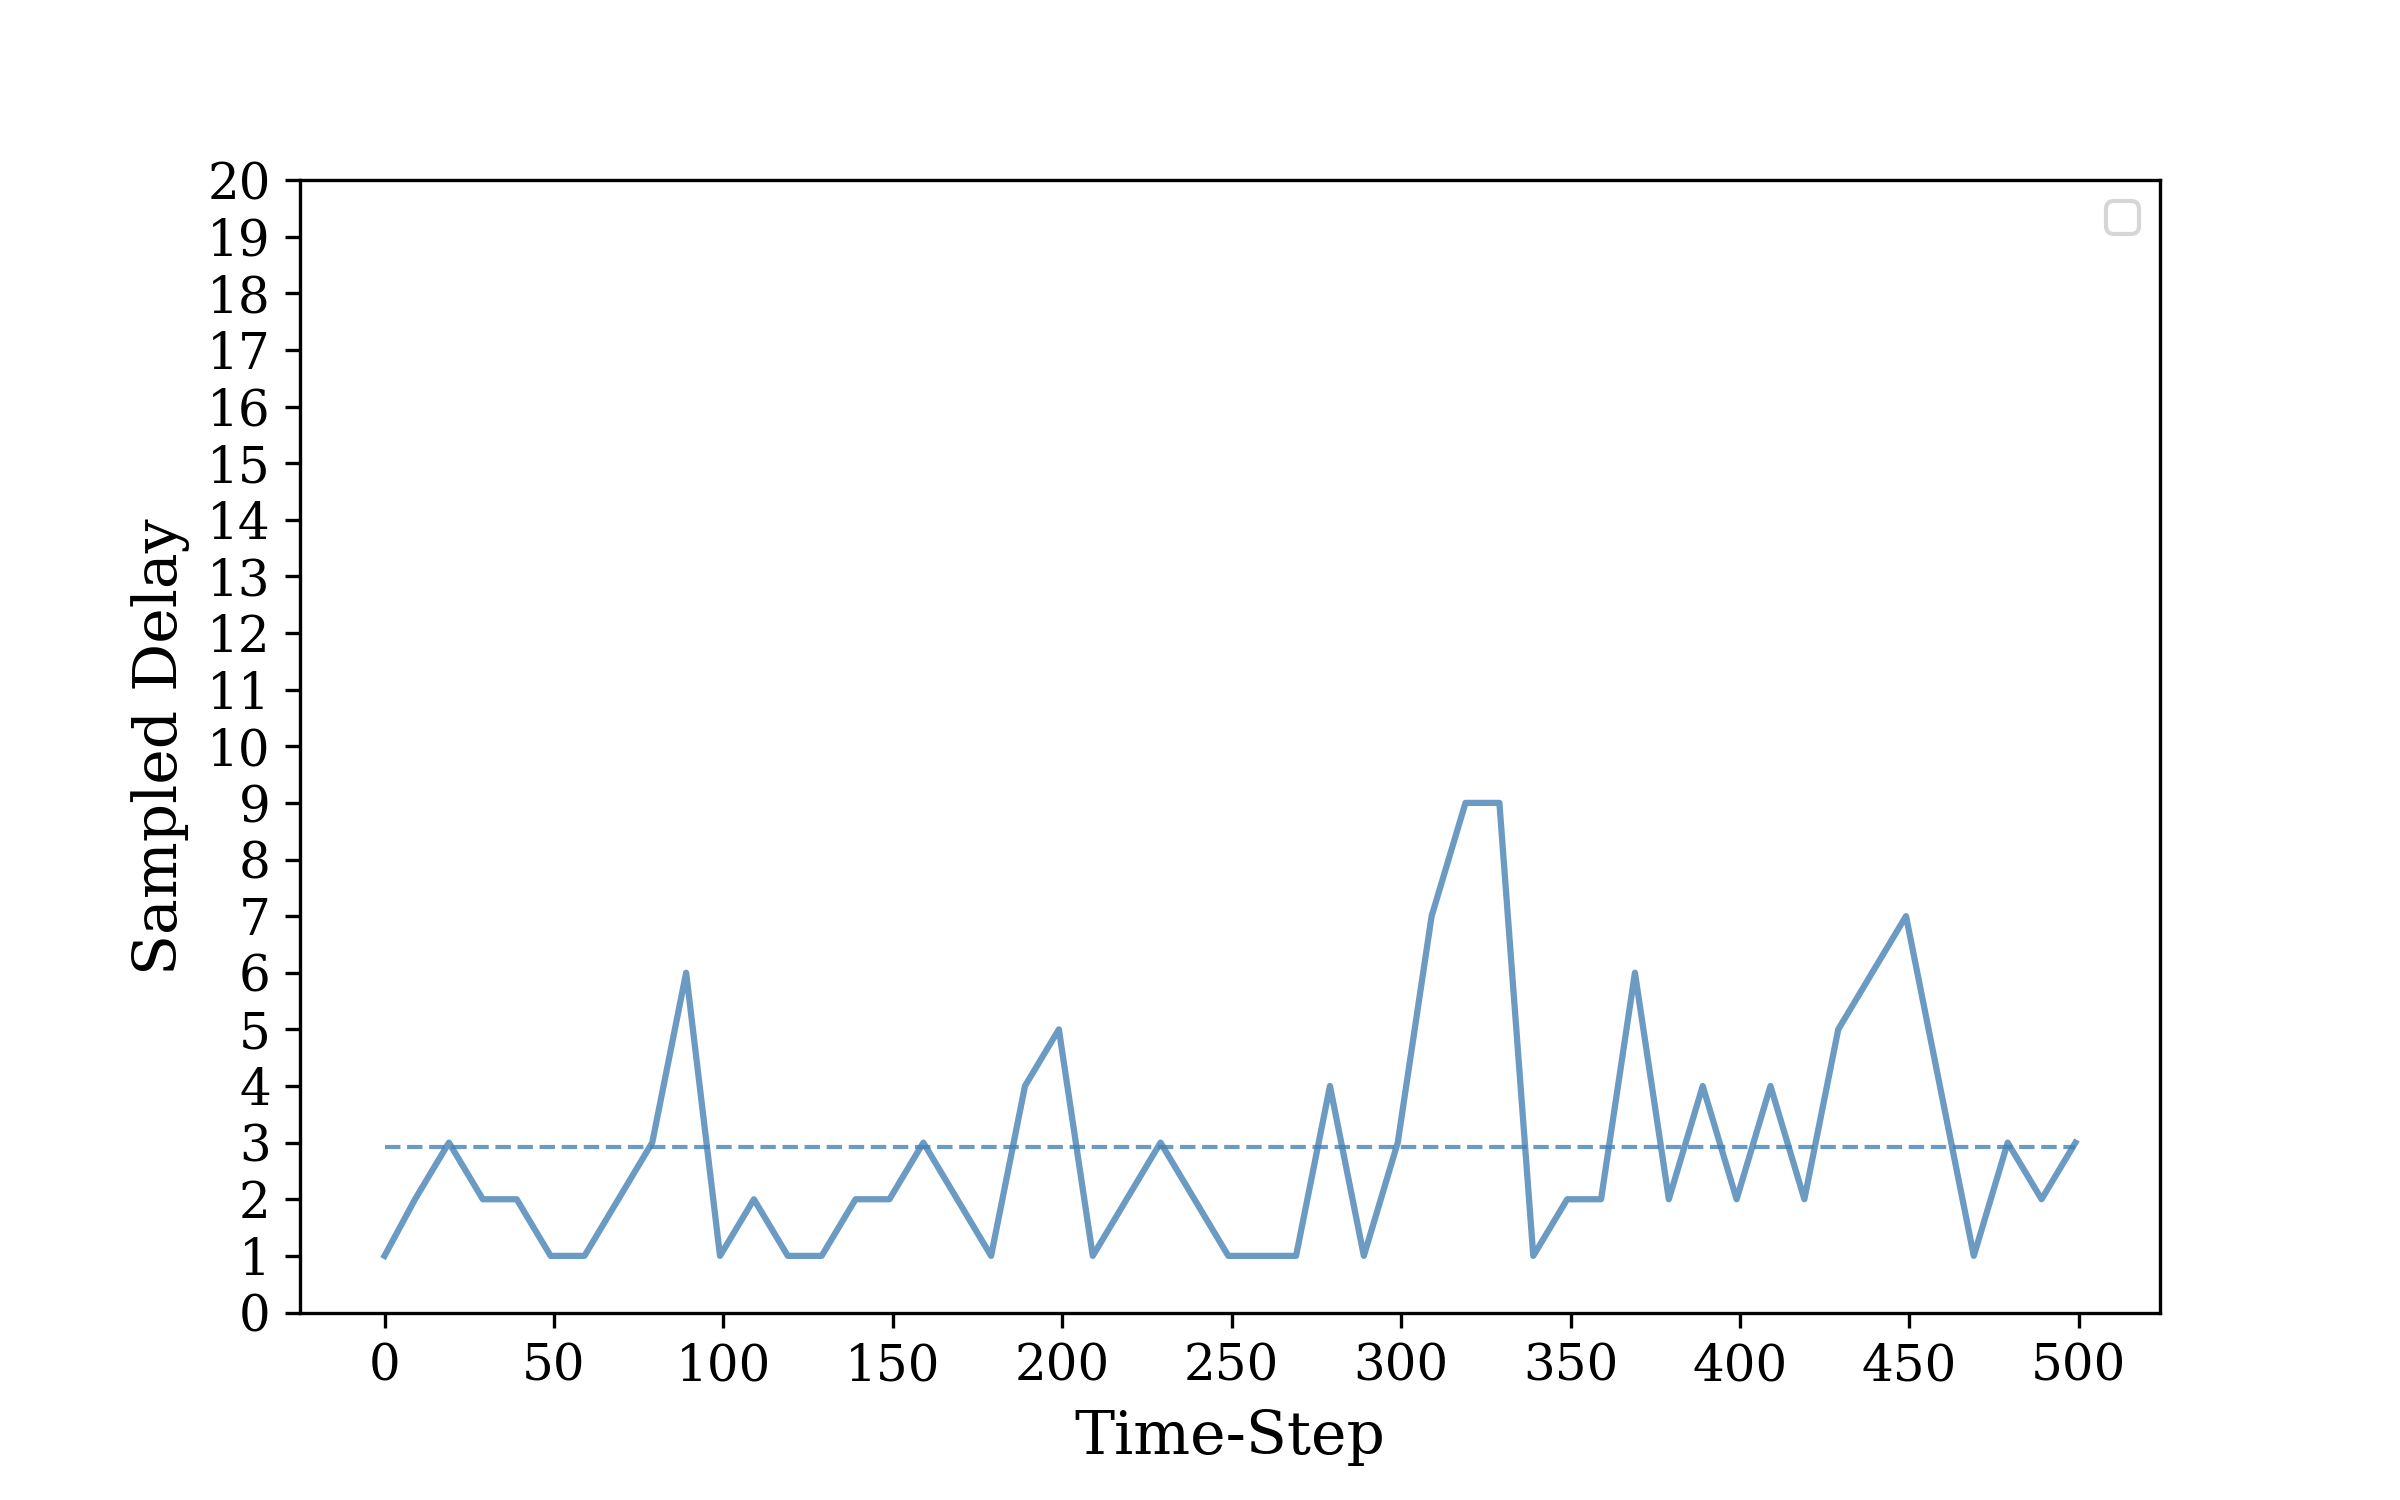
\includegraphics[width=11cm]{images/results/delayp07_sampledelay_1.png}
                    \caption{An instance of the stochastic jump process that generates the amount of delay with $p = 0.7$. The average delay sampled is highlighted by the dashed line.}
                    \label{fig:delayp07_sampledelay}
                    
                    \centering 
                    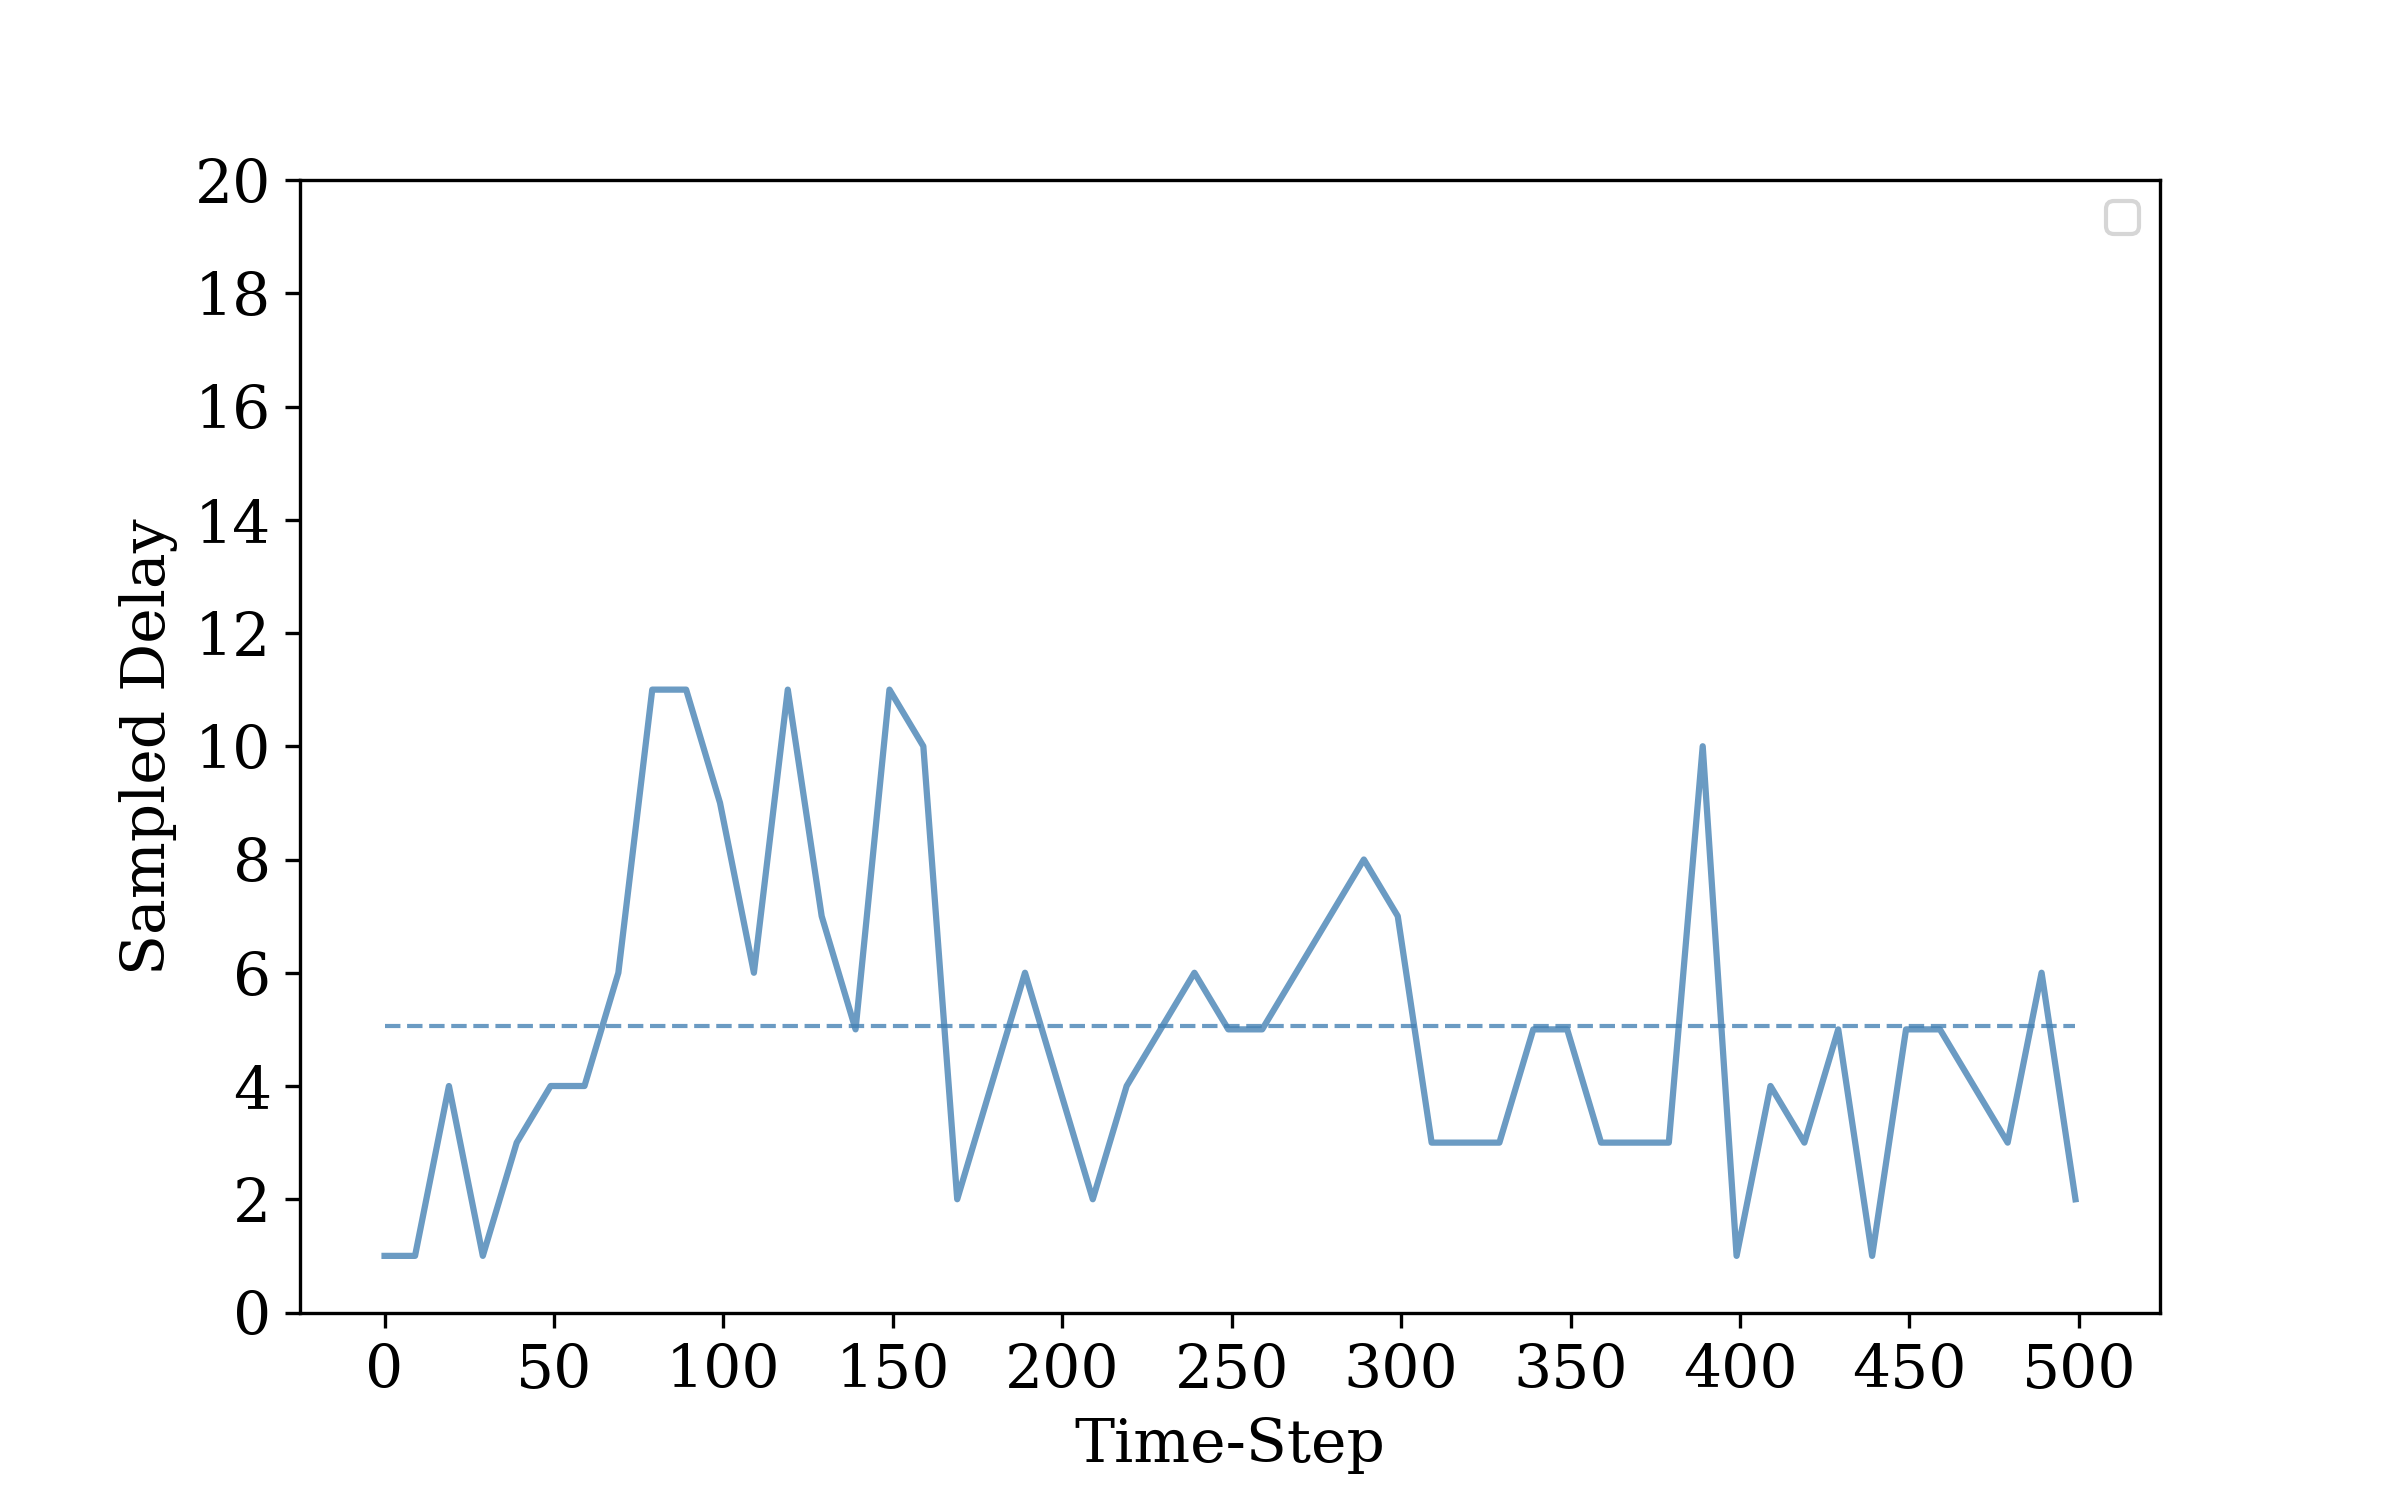
\includegraphics[width=11cm]{images/results/delayp06_sampledelay_1.png}
                    \caption{An instance of the stochastic jump process that generates the amount of delay with $p = 0.6$. The average delay sampled is highlighted by the dashed line.}
                    \label{fig:delayp06_sampledelay}
                    
                    \centering
                    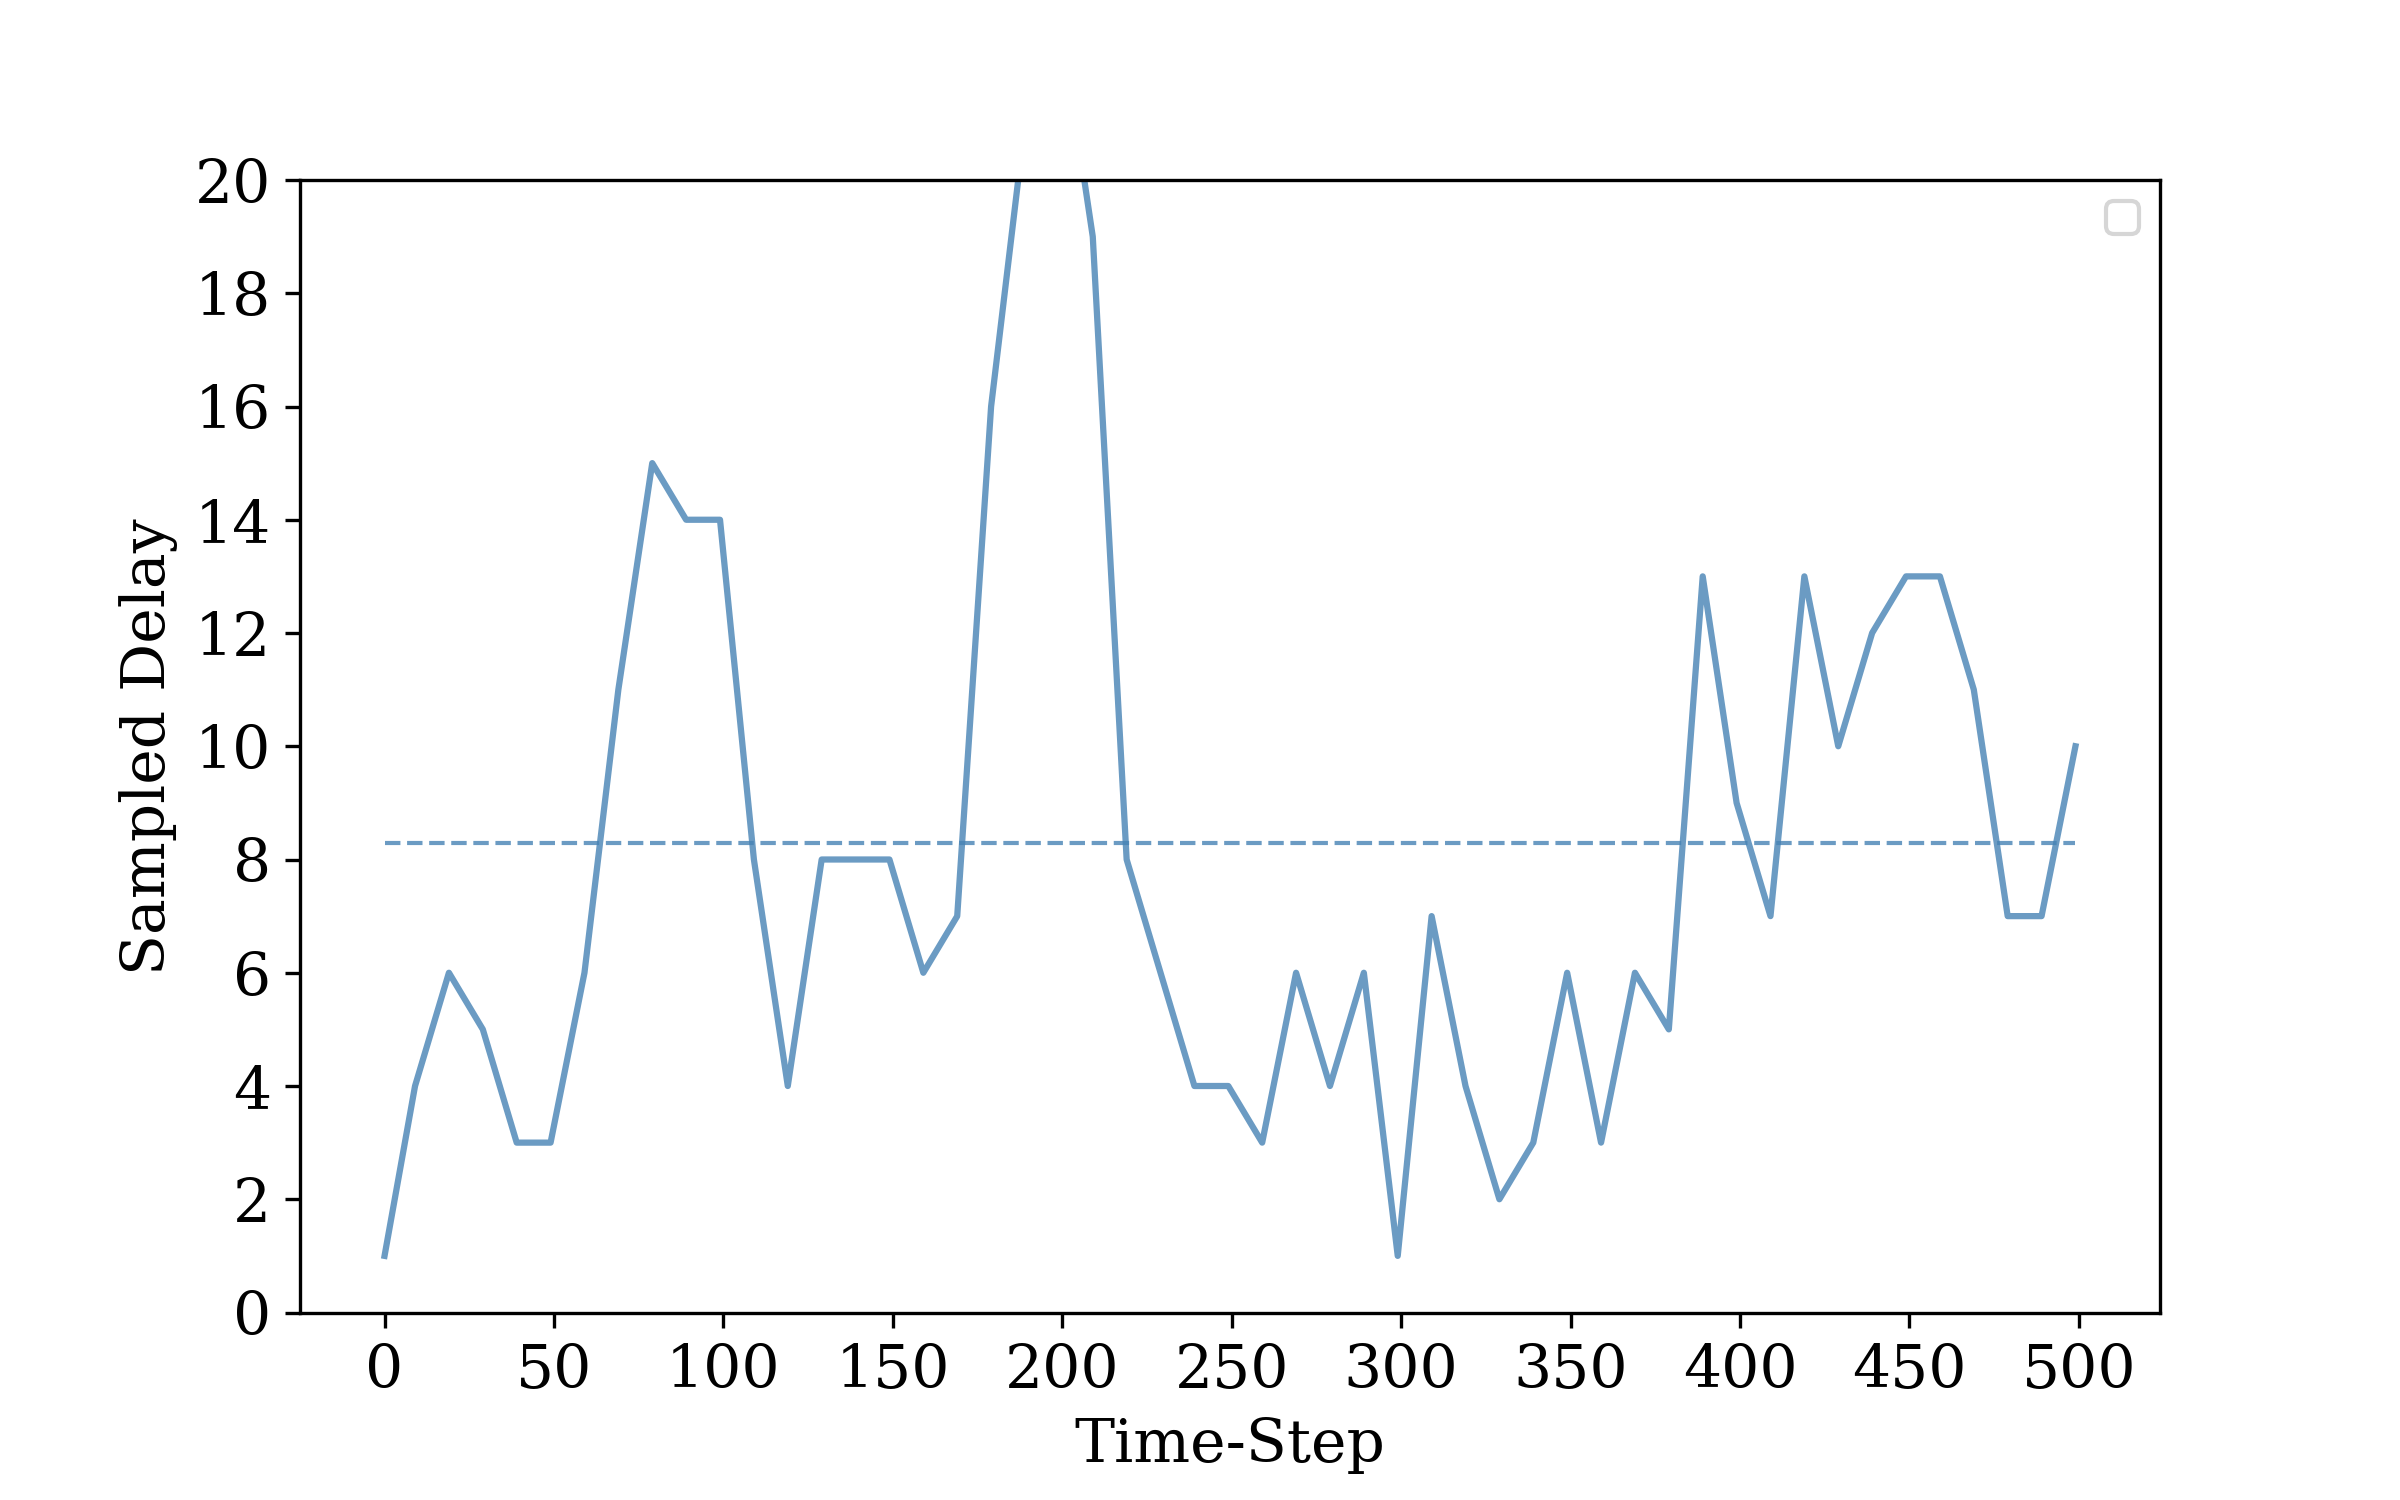
\includegraphics[width=11cm]{images/results/delayp05_sampledelay_1.png}
                    \caption{An instance of the stochastic jump process that generates the amount of delay with $p = 0.5$. The average delay sampled is highlighted by the dashed line.}
                    \label{fig:delayp05_sampledelay}
                \end{figure}
                
        \subsection{Baselines}
        \label{sub:baselines}
        % Dedicated to explain the baseline algorithms used through all tests
            In order to properly estimated the proposed algorithms' performances, we need to define baseline algorithms and evaluate their performance in the same context. However, given the presence of delays, standard state-of-the-art Reinforcement Learning algorithm cannot be directly deployed as baselines. They need to be adapted through one of the approaches dedicated to the DMDP framework, presented in Section \ref{sota:delay_approaches}. We decided to adapt TRPO algorithm to the augmented and memoryless approach to have a direct comparison with our model-based approach of L2-TRPO and D-TRPO. We also implemented SARSA and d-SARSA as additional memoryless approach baselines. \newline
            It is important to mention that A-TRPO and d-SARSA are not able to cope with stochastic delays, due to the structure of the feedforward networks that implements Policy and Value functions, which is not able to handle variable-size inputs. For this reason, experiments involving stochastic delays are only concerned with L2-TRPO and D-TRPO performances.
            
            \subsubsection{Augmented Approach: A-TRPO}
                We refer to TRPO adaptation to the augmented approach as Augmented TRPO or A-TRPO. At each time-step $t$, the Agent observes the extended state $i_t$, selects an action $a_t$, action $a_{t-d}$ is executed and the Agent receives the delayed reward $r_t = \mathbf{R}(s_{t-d}, a_{t-d})$. In practice, TRPO algorithm is deployed to learn upon the augmented MDP resulting from the original DMDP, as explained in Section \ref{subs:augmentedapproach}. TRPO implementation is the same used for L2-TRPO and D-TRPO.
                
            \subsubsection{Memoryless Approach: M-TRPO}
                We refer to TRPO adaptation to the memoryless approach as Memoryless TRPO or M-TRPO. At each time-step $t$, the Agent observes the state $s_{t-d}$, selects an action $a_t$, action $a_{t-d}$ is executed and the Agent receives the delayed reward $r_t = \mathbf{R}(s_{t-d}, a_{t-d})$. Thus, TRPO is deployed to learn action selection in the environment observing only the last known state, ignoring the presence of delay, as explained in Section \ref{subs:memorylessapproach}. TRPO implementation is the same used for L2-TRPO and D-TRPO.
                
                
            \subsubsection{Memoryless Approach: SARSA and d-SARSA}
            % Note: Discretized State Space
                At last, we wanted to compare our original algorithms against a specific algorithm from the literature. We chose d-SARSA, presented in Section \ref{subs:memorylessapproach}, as a memoryless algorithm that achieved good results. Along with it, given its easy implementation, we also decided to test the original SARSA algorithm in the context of memoryless approach. \newline
                In order to deploy SARSA and d-SARSA with environments characterized by continuous state and/or action space, such as Inverted Pendulum, it is necessary to discretize them. In our tests, both SARSA and d-SARSA learns upon a grid-discretized State Space of 15x15x15 and a discretized Action Space of 3 values.
                
                
    \newpage
    \section{Module Parameters Tuning}
    \label{results:module_tuning}
    % Section dedicated to the process of finding which parameters influences Module's performances and most affect the total number of parameter. We want to find the best trade-off, given the fact that each sample will be processed through the Encoder.
    %   - Tests on older version of the Module
    %   - Encoder Dim vs Encoder FF Dim vs Encoder Layers
    %   - Select only relevant plots for the comparison
        The first step in the process of evaluating the original implementation is assessing the module's properties: which are the hyperparameters that affect performances and total number of parameters the most. The goal of this section is to understand which hyperparameters offer the best trade-off between performance gains and number of additional parameters in the module. Given the fact that the module is involved in computing the state or belief representation at each time-step, optimizing the total number of parameters is a key factor in order not to slow down the training process to a point in which the modules' benefits are sinked by long training times. \newline
        The following tests are performed on the State-Prediction module, which is trained for 200 epochs, each composed by 100 trajectories of 250 steps, for a total of 5 million steps. Each module has been trained 3 times with 3 different seeds, the results are presented as averages between them. In order to concisely refer to each of the modules tested, we set up a bit of nomenclature: each module will be referred to as [$enc_{ff}$, $enc_{dim}$, $e$], which are the Transformer Encoder's feedforward dimension, internal dimension and number of encoder layers respectively. 
        
        \subsection{Cross-Validation}
        % Describe the first test with all Encoders between [16, 16, 1] and [32, 32, 2]
            In this test, we start with two reference modules [32, 32, 2] and [16, 16, 1] and we evaluate the performance difference between them and the sequence of modules obtained by lowering one hyperparameter at a time: [16, 32, 2]; [32, 16, 2] and [32, 32, 1]. Figure \ref{fig:results_parametertuning_1} shows the results of the test and Figure \ref{fig:results_parametertuning_2} focuses on the last epochs of training for a better illustration of the differences between the modules. \newline
            As expected, modules [16, 16, 1] and [32, 32, 2] are respectively the worst and best modules performance-wise, but [32, 32, 2] also has approximately 7 times the number of parameters. As for the other tested modules, we can break down conclusions for each of them:
            \begin{itemize}
                \item Module [16, 32, 2] with 12227 parameters: lowering $enc_{ff}$ from 32 to 16 does not affect the module performance-wise and results in a loss of 14.5\% parameters, possibly indicating that $enc_{ff}$ is not crucial for the module capabilities.
                \item Module [32, 16, 2] with 4483 parameters: lowering $enc_{dim}$ from 32 to 16 hugely affects the module's performances, which become closer to [16, 16, 1] then any other module, possibly indicating that the parameter plays a very important role in the module capabilities. As expected, since $enc_{dim}$ directly affect the matrices' dimensions in the Self-Attention network, the number of total parameter is greatly reduced by 65.9\%.
                \item Module [32, 32, 1] with 7843 parameters: lowering the number of encoder layers has a mild effect on module's performances, with a loss of 45.2\% of the parameters, possibly indicating an intermediate importance between the other two parameters.
            \end{itemize}
            \noindent
            From the results of these tests, we can state that $enc_{dim}$ and $e$ are influencing both module's performances and total number of parameters significantly, while $enc_{ff}$ is not as influential and it may be decresed in favor of less total parameters. Looking at the module design, this result is reasonable: $enc_{dim}$ directly affects the number of parameters used to compute the attention scores, while $e$ determines how many encoder layers are used on top of each other. However, even if lowering $enc_{dim}$ has impacted performances more, we also need to observe that the total number of parameters has also diminished drastically. The next Section is concerned with a test to properly assess which of the two parameters offer the best trade-off between computational complexity and performances.
        
        \subsection{Performance Scaling Test}
        % Describe the second test between [8, 192, 2] - 343507; [8, 256, 1] - 336907 and [8, 512, 1] - 1329163
            This second test is aimed at establishing which parameter offers the best trade-off between $enc_{dim}$ and $e$ as well as observing how the module's performances scale with them. For this reason, we test three new modules: [8, 192, 2] with 343507 parameters; [8, 256, 1] with 336907 and [8, 512, 1] with 1329163 parameters. Figures \ref{fig:results_scalability_1} and \ref{fig:results_scalability_2} illustrate the result of this test. \newline
            At first, we focus on [8, 192, 2] and [8, 256, 1]: both modules offer almost the same number of parameters in contrast to the previous test. However, [8, 256, 1] is clearly faster to learn and it can reach a slightly better loss value. Even if the difference is not great, we decide to give priority to $enc_{dim}$, also given its meaning within the module's architecture. Also, we can observe that lowering $enc_{ff}$ to 8 hasn't impacted the module's performances in both cases. \newline
            At last, it is possible to observe that module [8, 512, 1] is showing increased speed to convergence and a slightly better loss value, indicating that it is possible to enlarge $enc_{dim}$ to 512 without encountering significant diminishing return effects.
        
        \subsection{ADAM Learning Rate}
            As explained in Section \ref{ow:deterministic_module} and \ref{ow:beliefmodule}, the module is trained using ADAM optimization algorithm. All tests shown so far are executed with a conservative learning rate of $10^{-4}$. After having established the most important parameters performance-wise, we want to decrease the total number of parameters required possibly maintaining the same level of performances, in order to speed up the learning process. For this reason, we want to test the module [8, 128, 1] with 86539 parameters trained with ADAM with larger learning rates: $10^{-1}$, $10^{-2}$ and $10^{-3}$; and we compare it to the previous trained module [8, 512, 1], trained with learning rate $10^{-4}$. Figures \ref{fig:results_lr_2} and \ref{fig:results_lr_1} show the results of the test. \newline
            In practice, the test shows that we are able to increase ADAM learning rate safely until a value of $10^{-2}$, since $10^{-1}$ shows lower and unstable performances. Furthermore, [8, 128, 1] is able to outperform [8, 512, 1] significantly with a proper learning rate value, while having a fraction of the total number of parameters.
            
        \subsection{Causal Option}
            As a last test, we want to establish the effects of the causal mask applied to the Self-Attention network of the module. To this purpose, we compare a new module [8, 128, 1] trained with the causal mask to [8, 128, 1] and [8, 512, 1]. Figures \ref{fig:results_causal_1} and \ref{fig:results_causal_2} illustrates the results of the test. \newline We conjecture that the causal mask allows the module to "concentrate" only on the correct portion of the input sequence while computing the attention vectors for each input element, thus avoiding a waste of time and resources by looking at the future elements that are not relevant. Results seems to confirm the hypothesis: the module trained with the causal mask is faster to converge and reaches a slightly better loss value overall.
        
        \begin{figure}[hbtp]
                \centering
                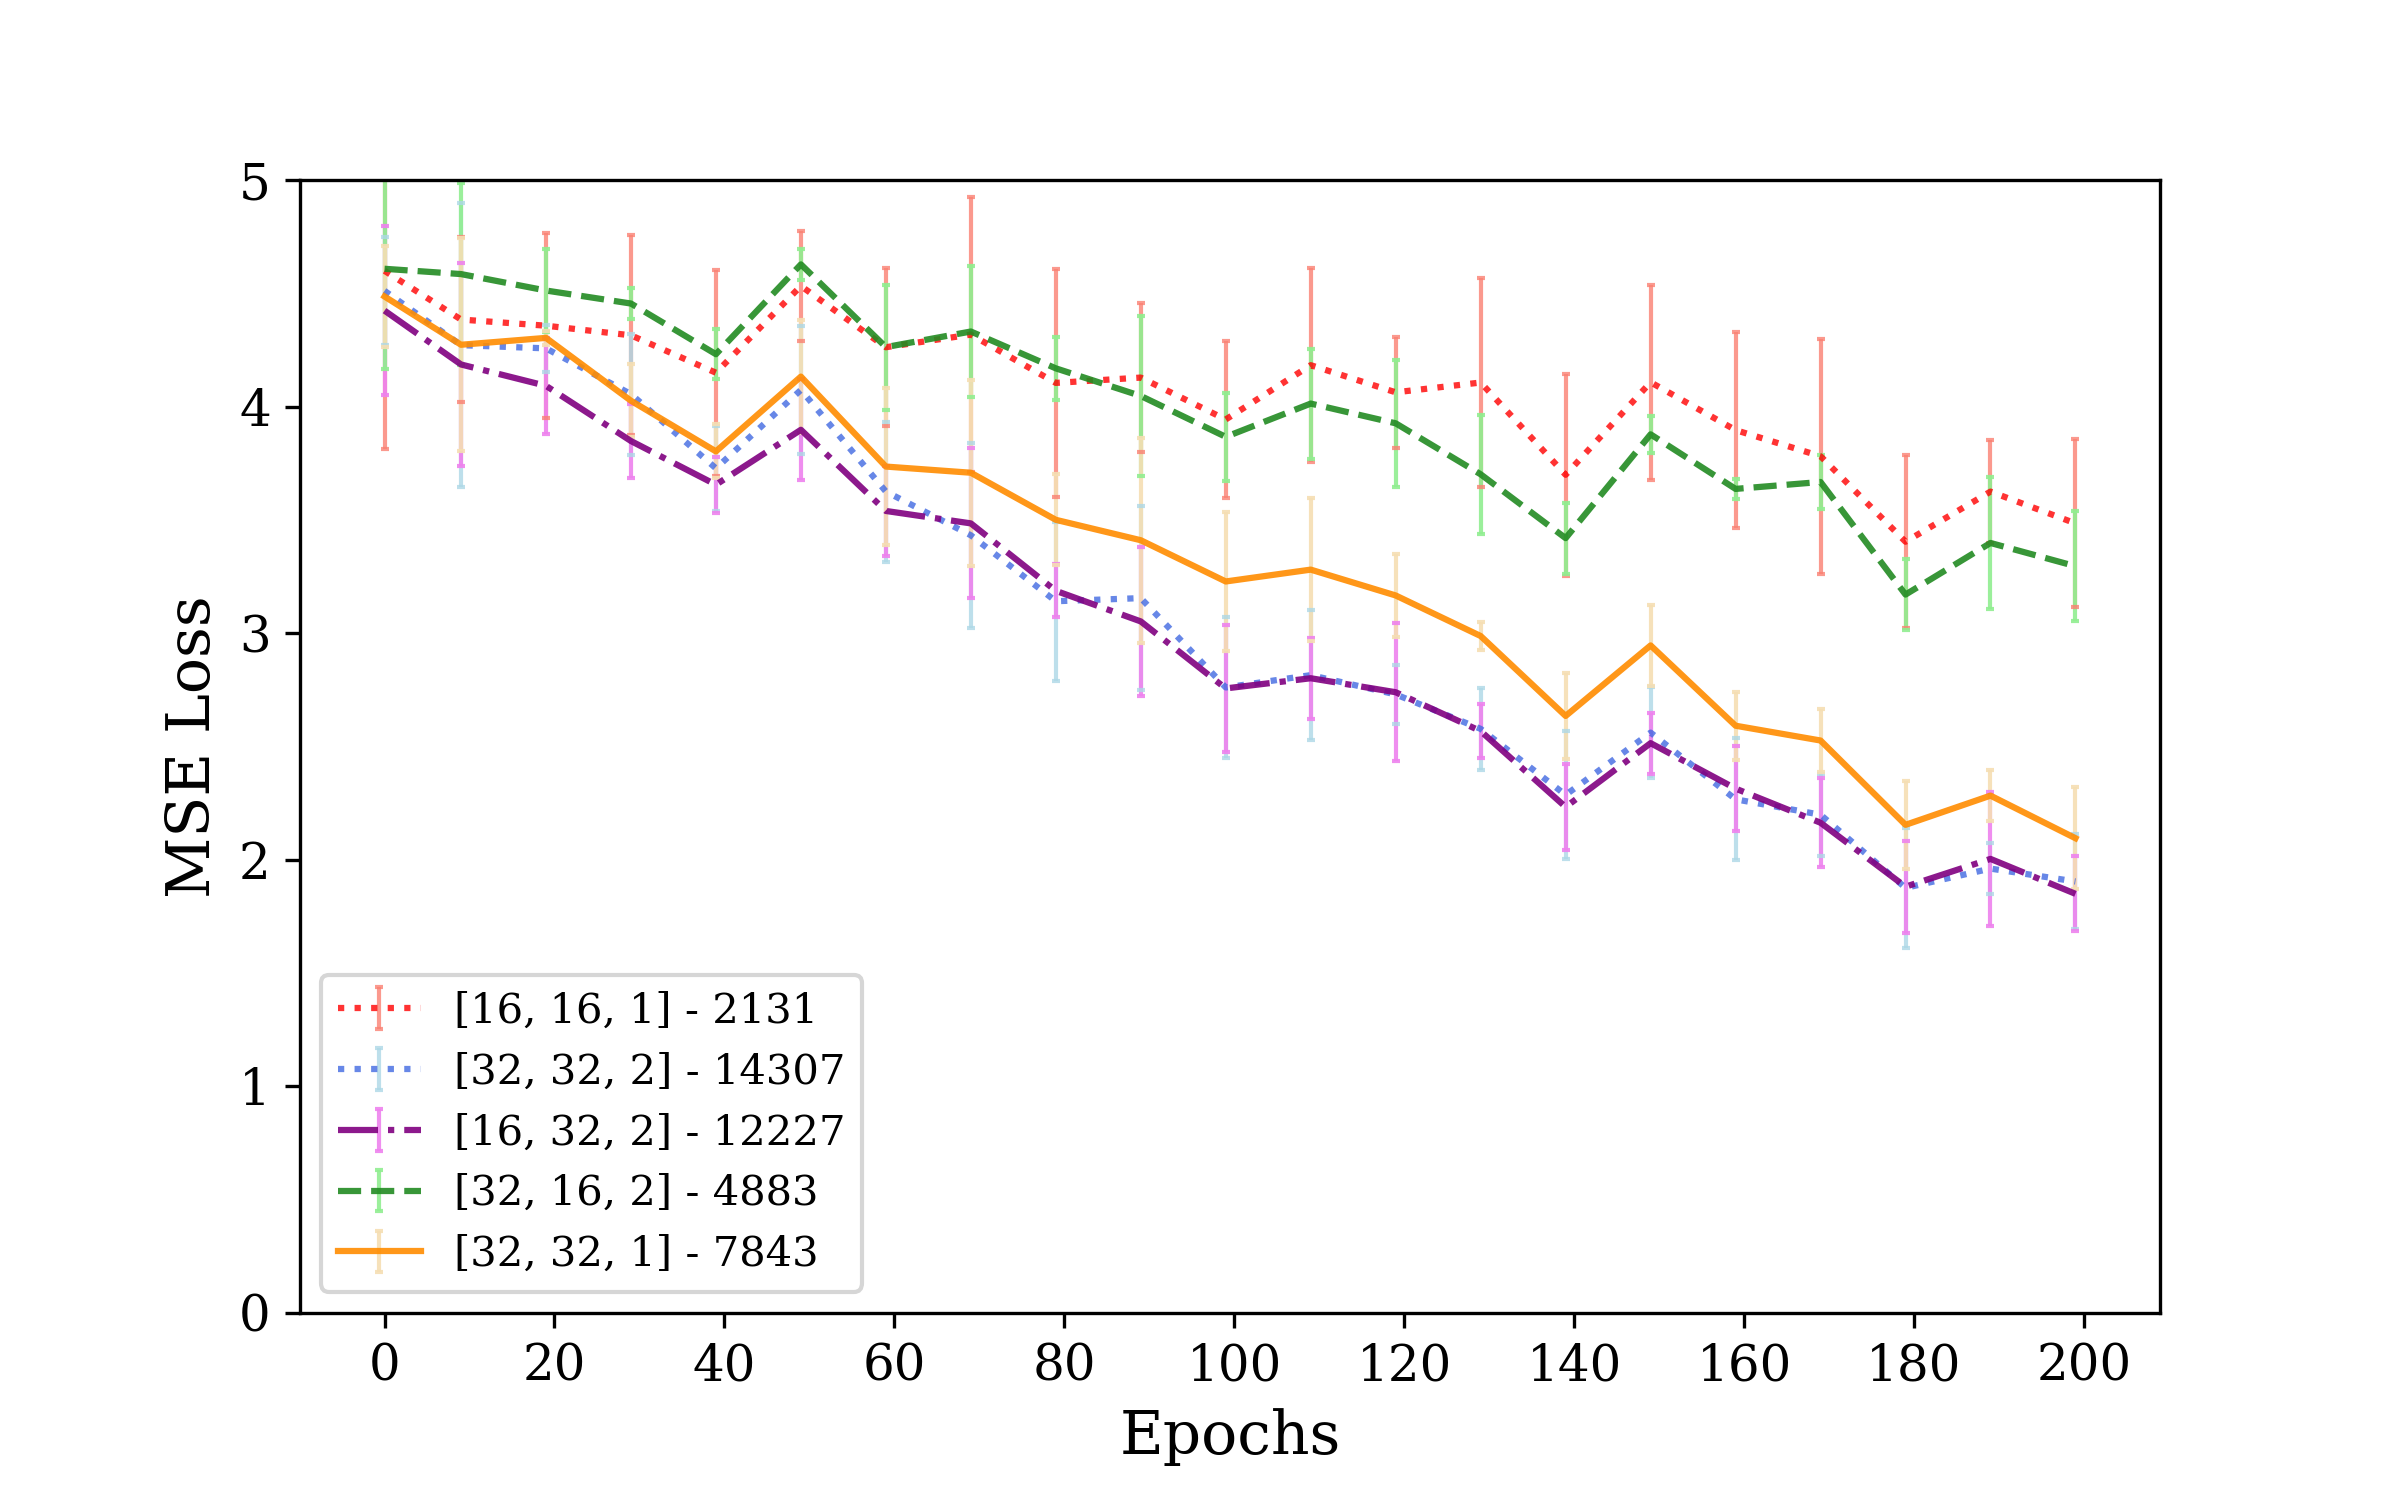
\includegraphics[width=15cm, keepaspectratio]{images/results/module_parametertuning_1.png}
                \caption{MSE Loss Function $L_{pred}$ of the trained modules. The right-hand side number in the legend is the total number of parameter of each module.}
                \label{fig:results_parametertuning_1}
                
                \vspace{1.5cm}
                
                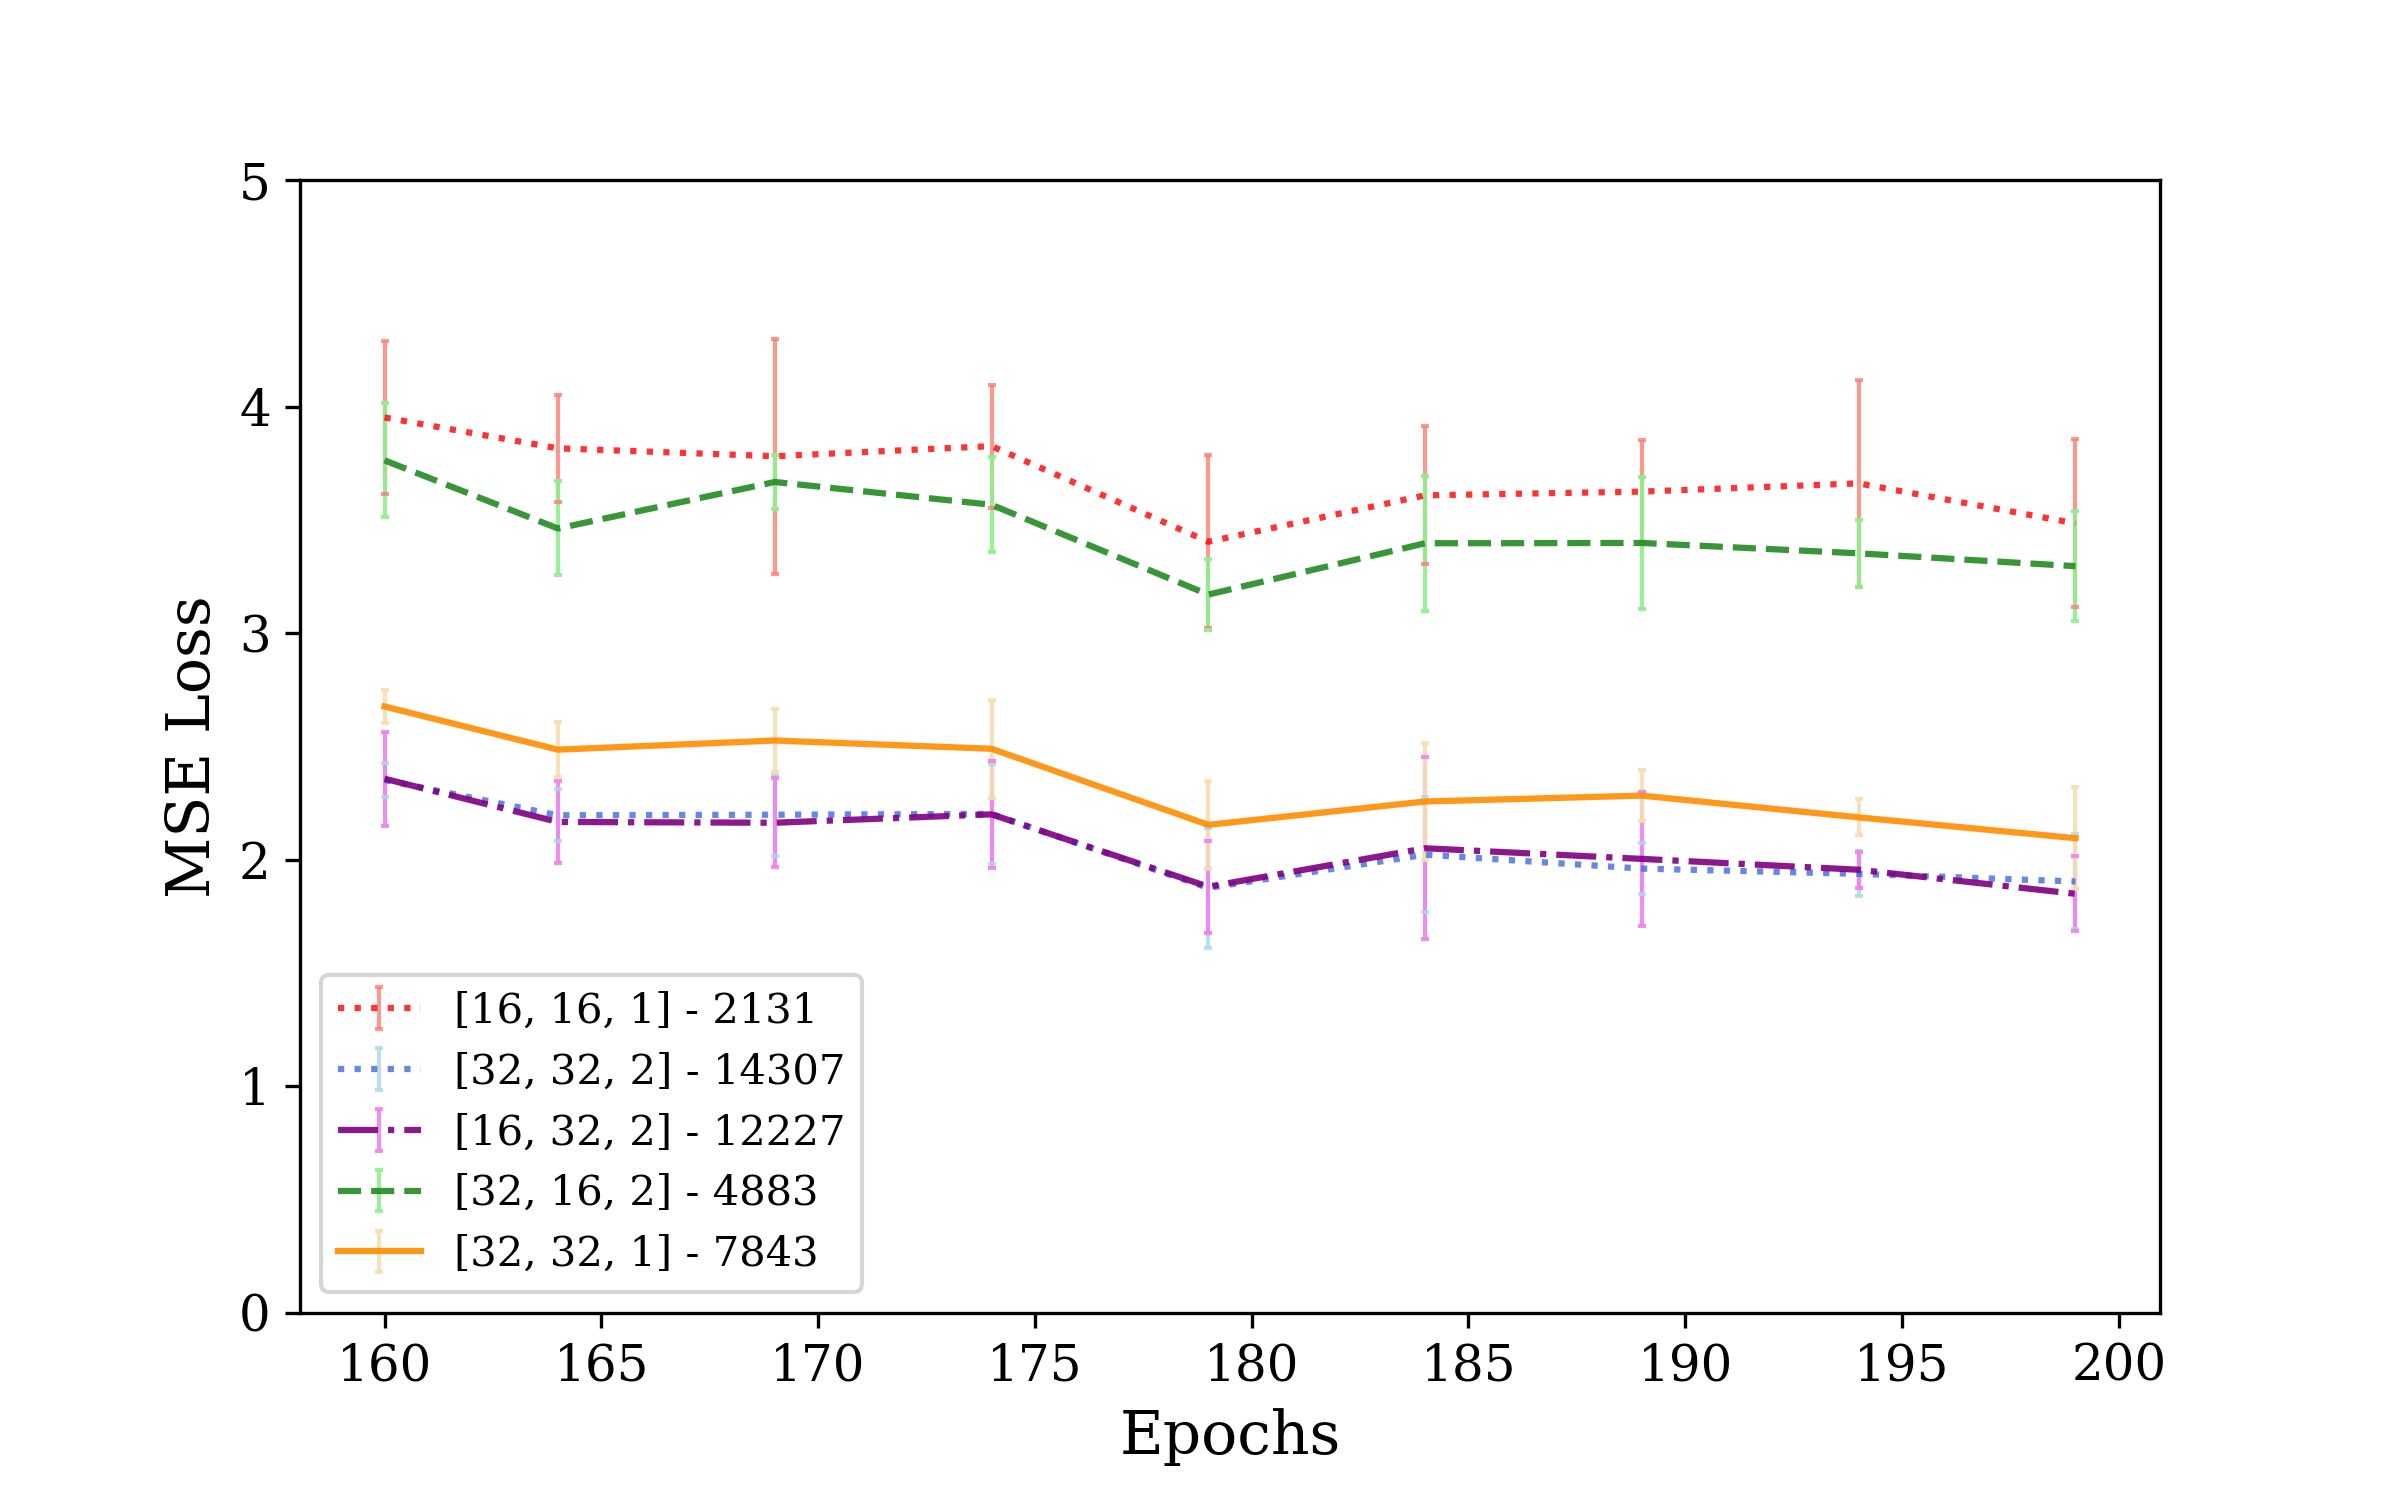
\includegraphics[width=15cm, keepaspectratio]{images/results/module_parametertuning_2.png}
                \caption{MSE Loss Function $L_{pred}$ of the trained modules between Epoch 160 and Epoch 200. The right-hand side number in the legend is the total number of parameter of each module.}
                \label{fig:results_parametertuning_2}
        \end{figure}
        
        \begin{figure}[hbtp]
                \centering
                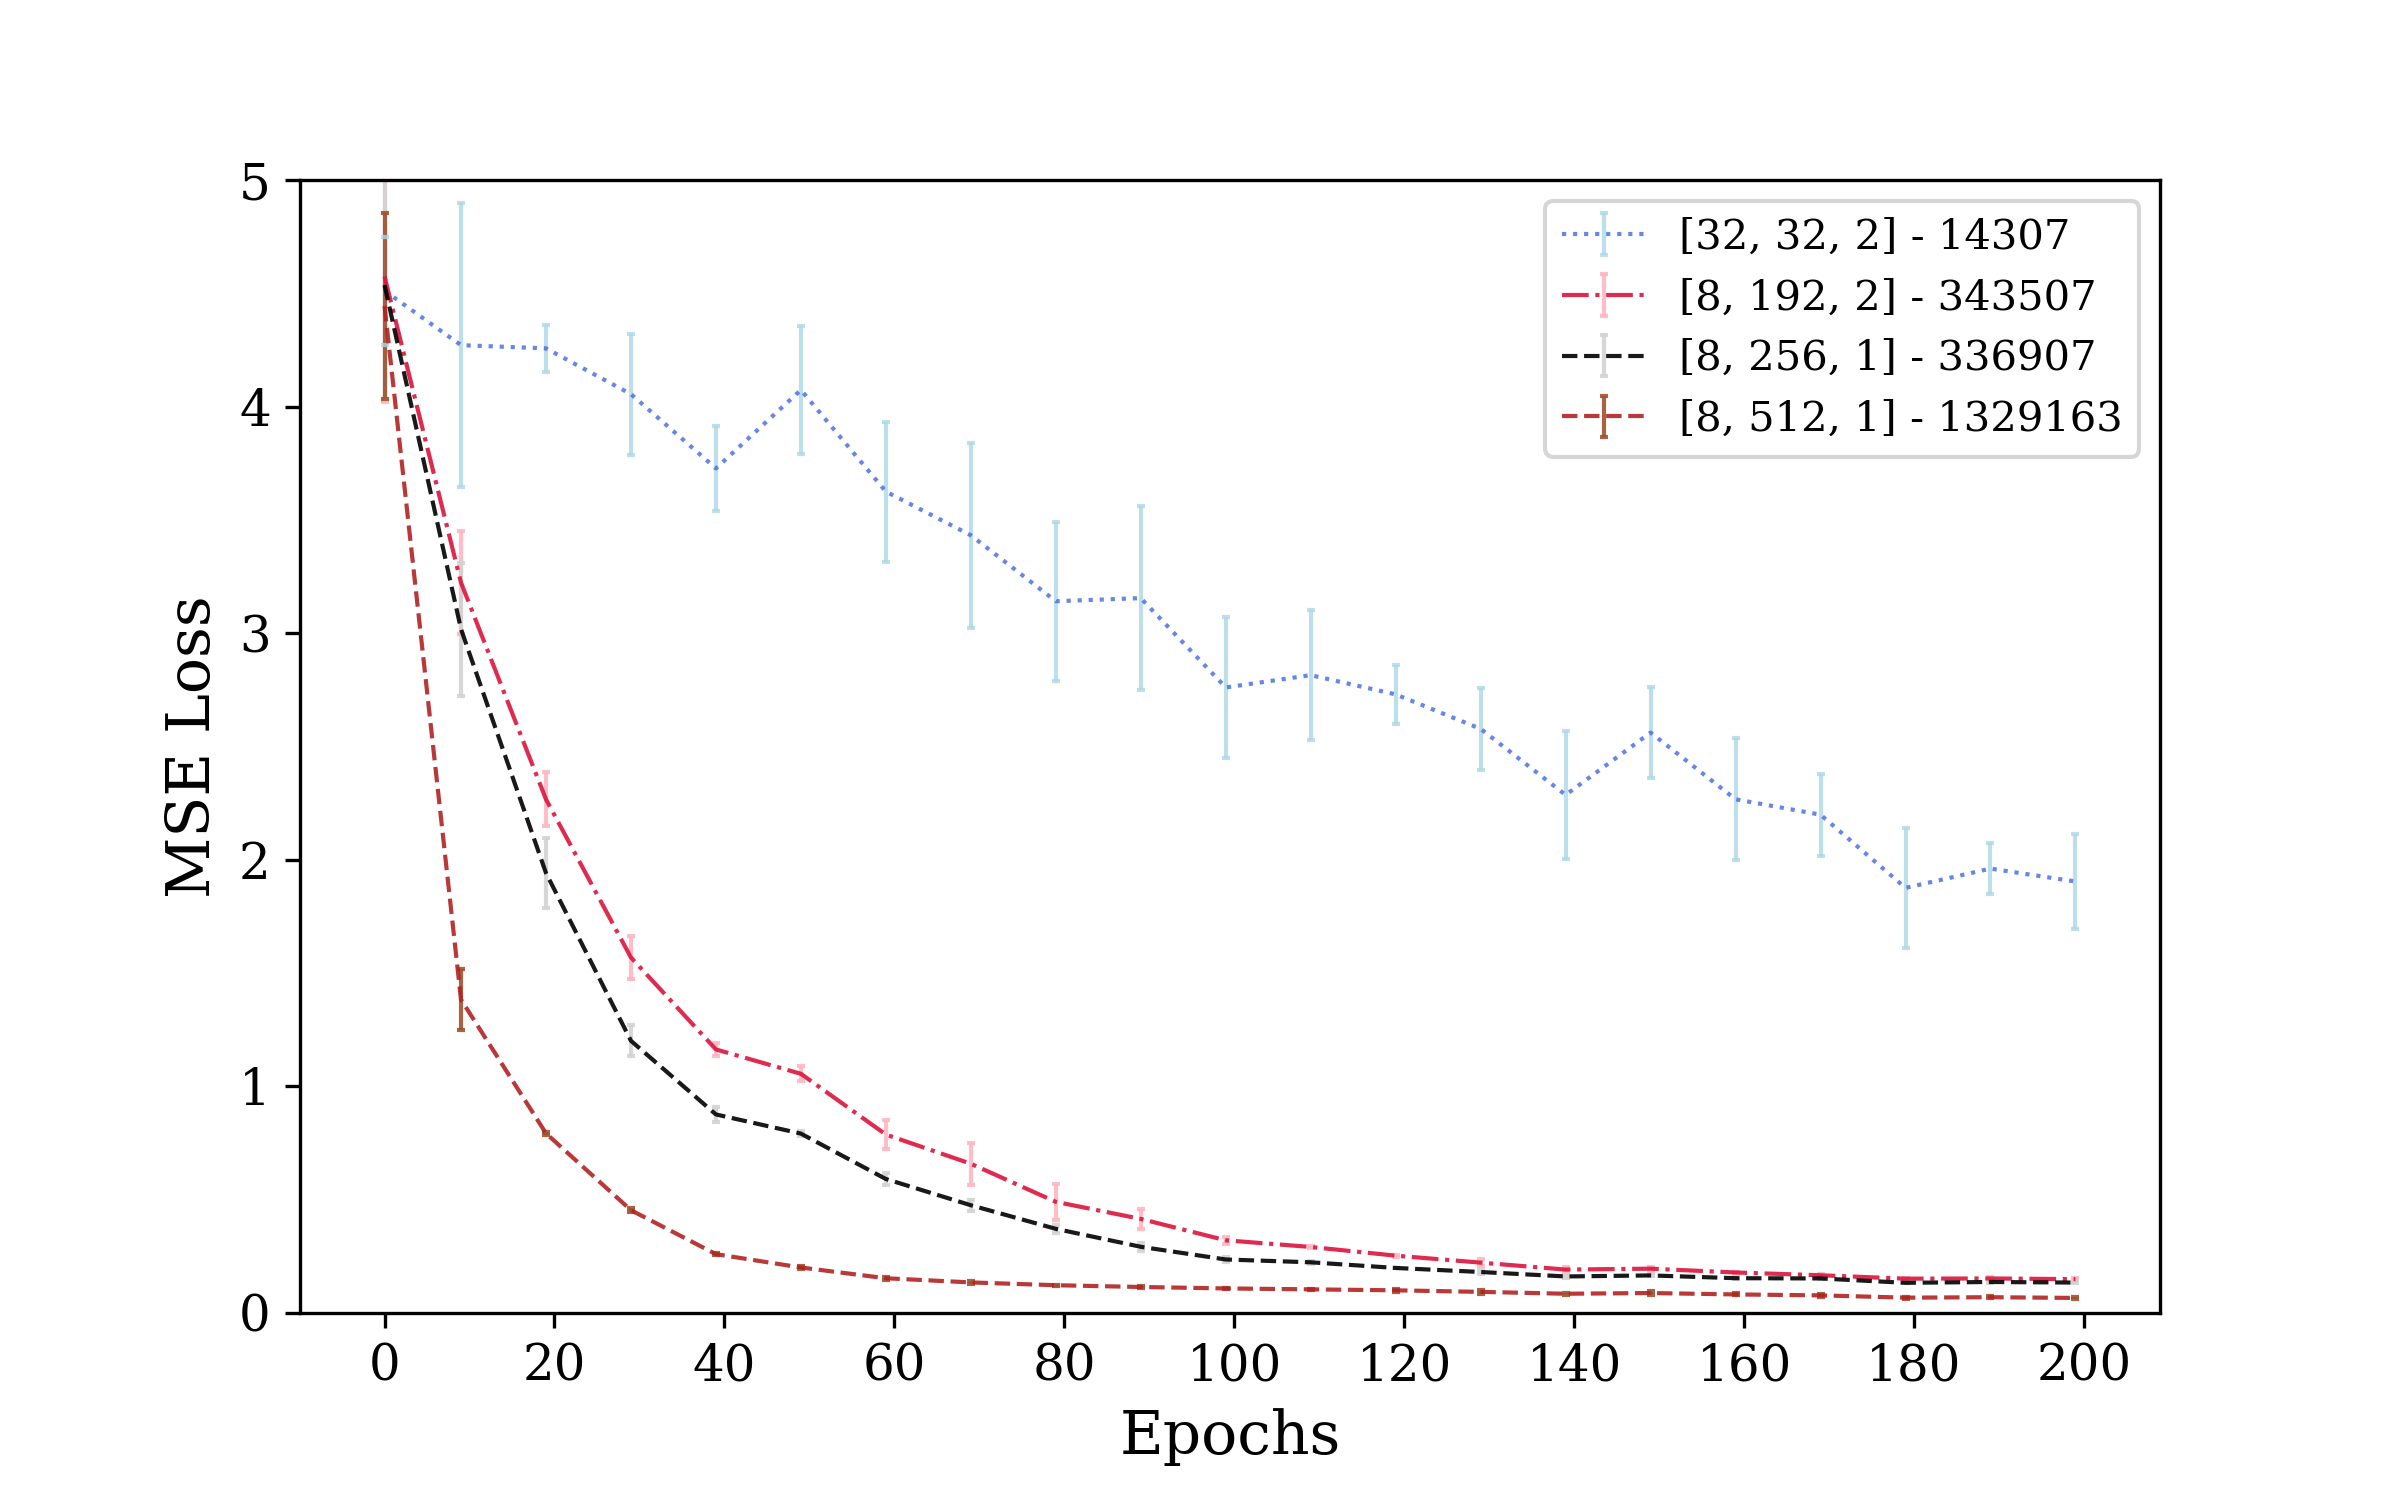
\includegraphics[width=15cm, keepaspectratio]{images/results/module_scalability_1.png}
                \caption{MSE Loss Function $L_{pred}$ of the trained modules. The right-hand side number in the legend is the total number of parameter of each module.}
                \label{fig:results_scalability_1}
                
                \vspace{1.5cm}
                
                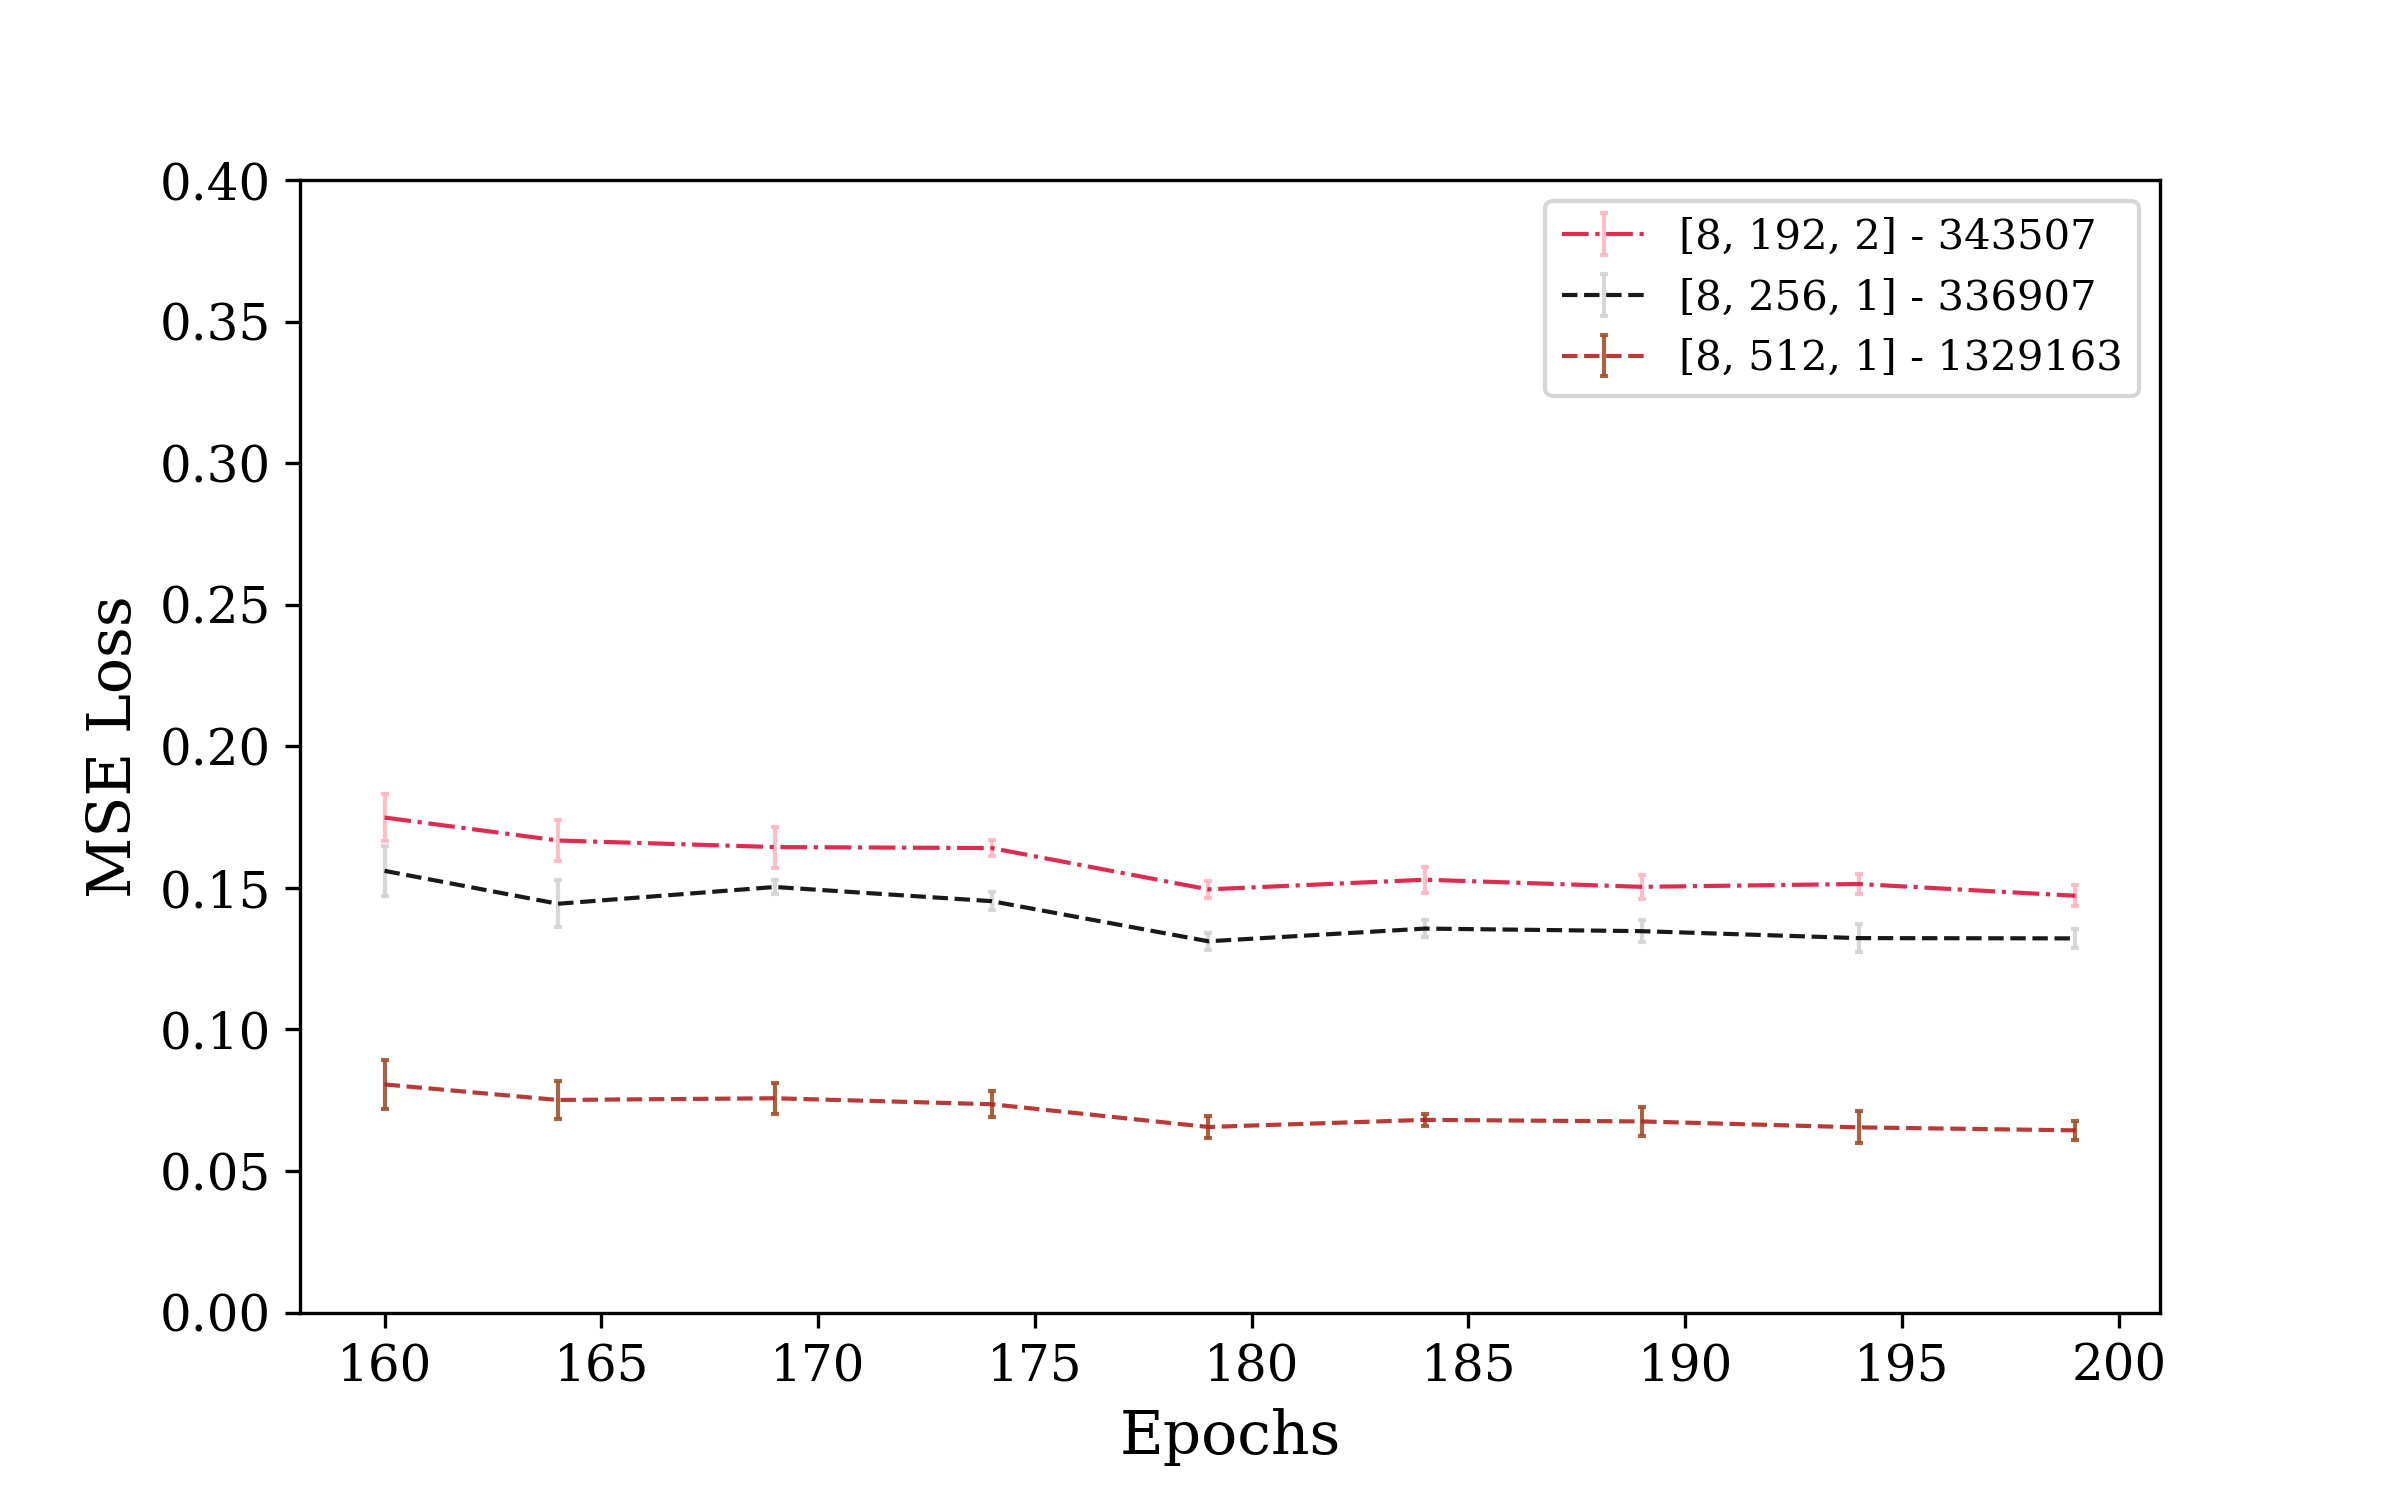
\includegraphics[width=15cm, keepaspectratio]{images/results/module_scalability_2.png}
                \caption{MSE Loss Function $L_{pred}$ of the trained modules between Epoch 160 and Epoch 200 for a better illustration. The right-hand side number in the legend is the total number of parameter of each module.}
                \label{fig:results_scalability_2}
        \end{figure}
        
        \begin{figure}[hbtp]
                \centering
                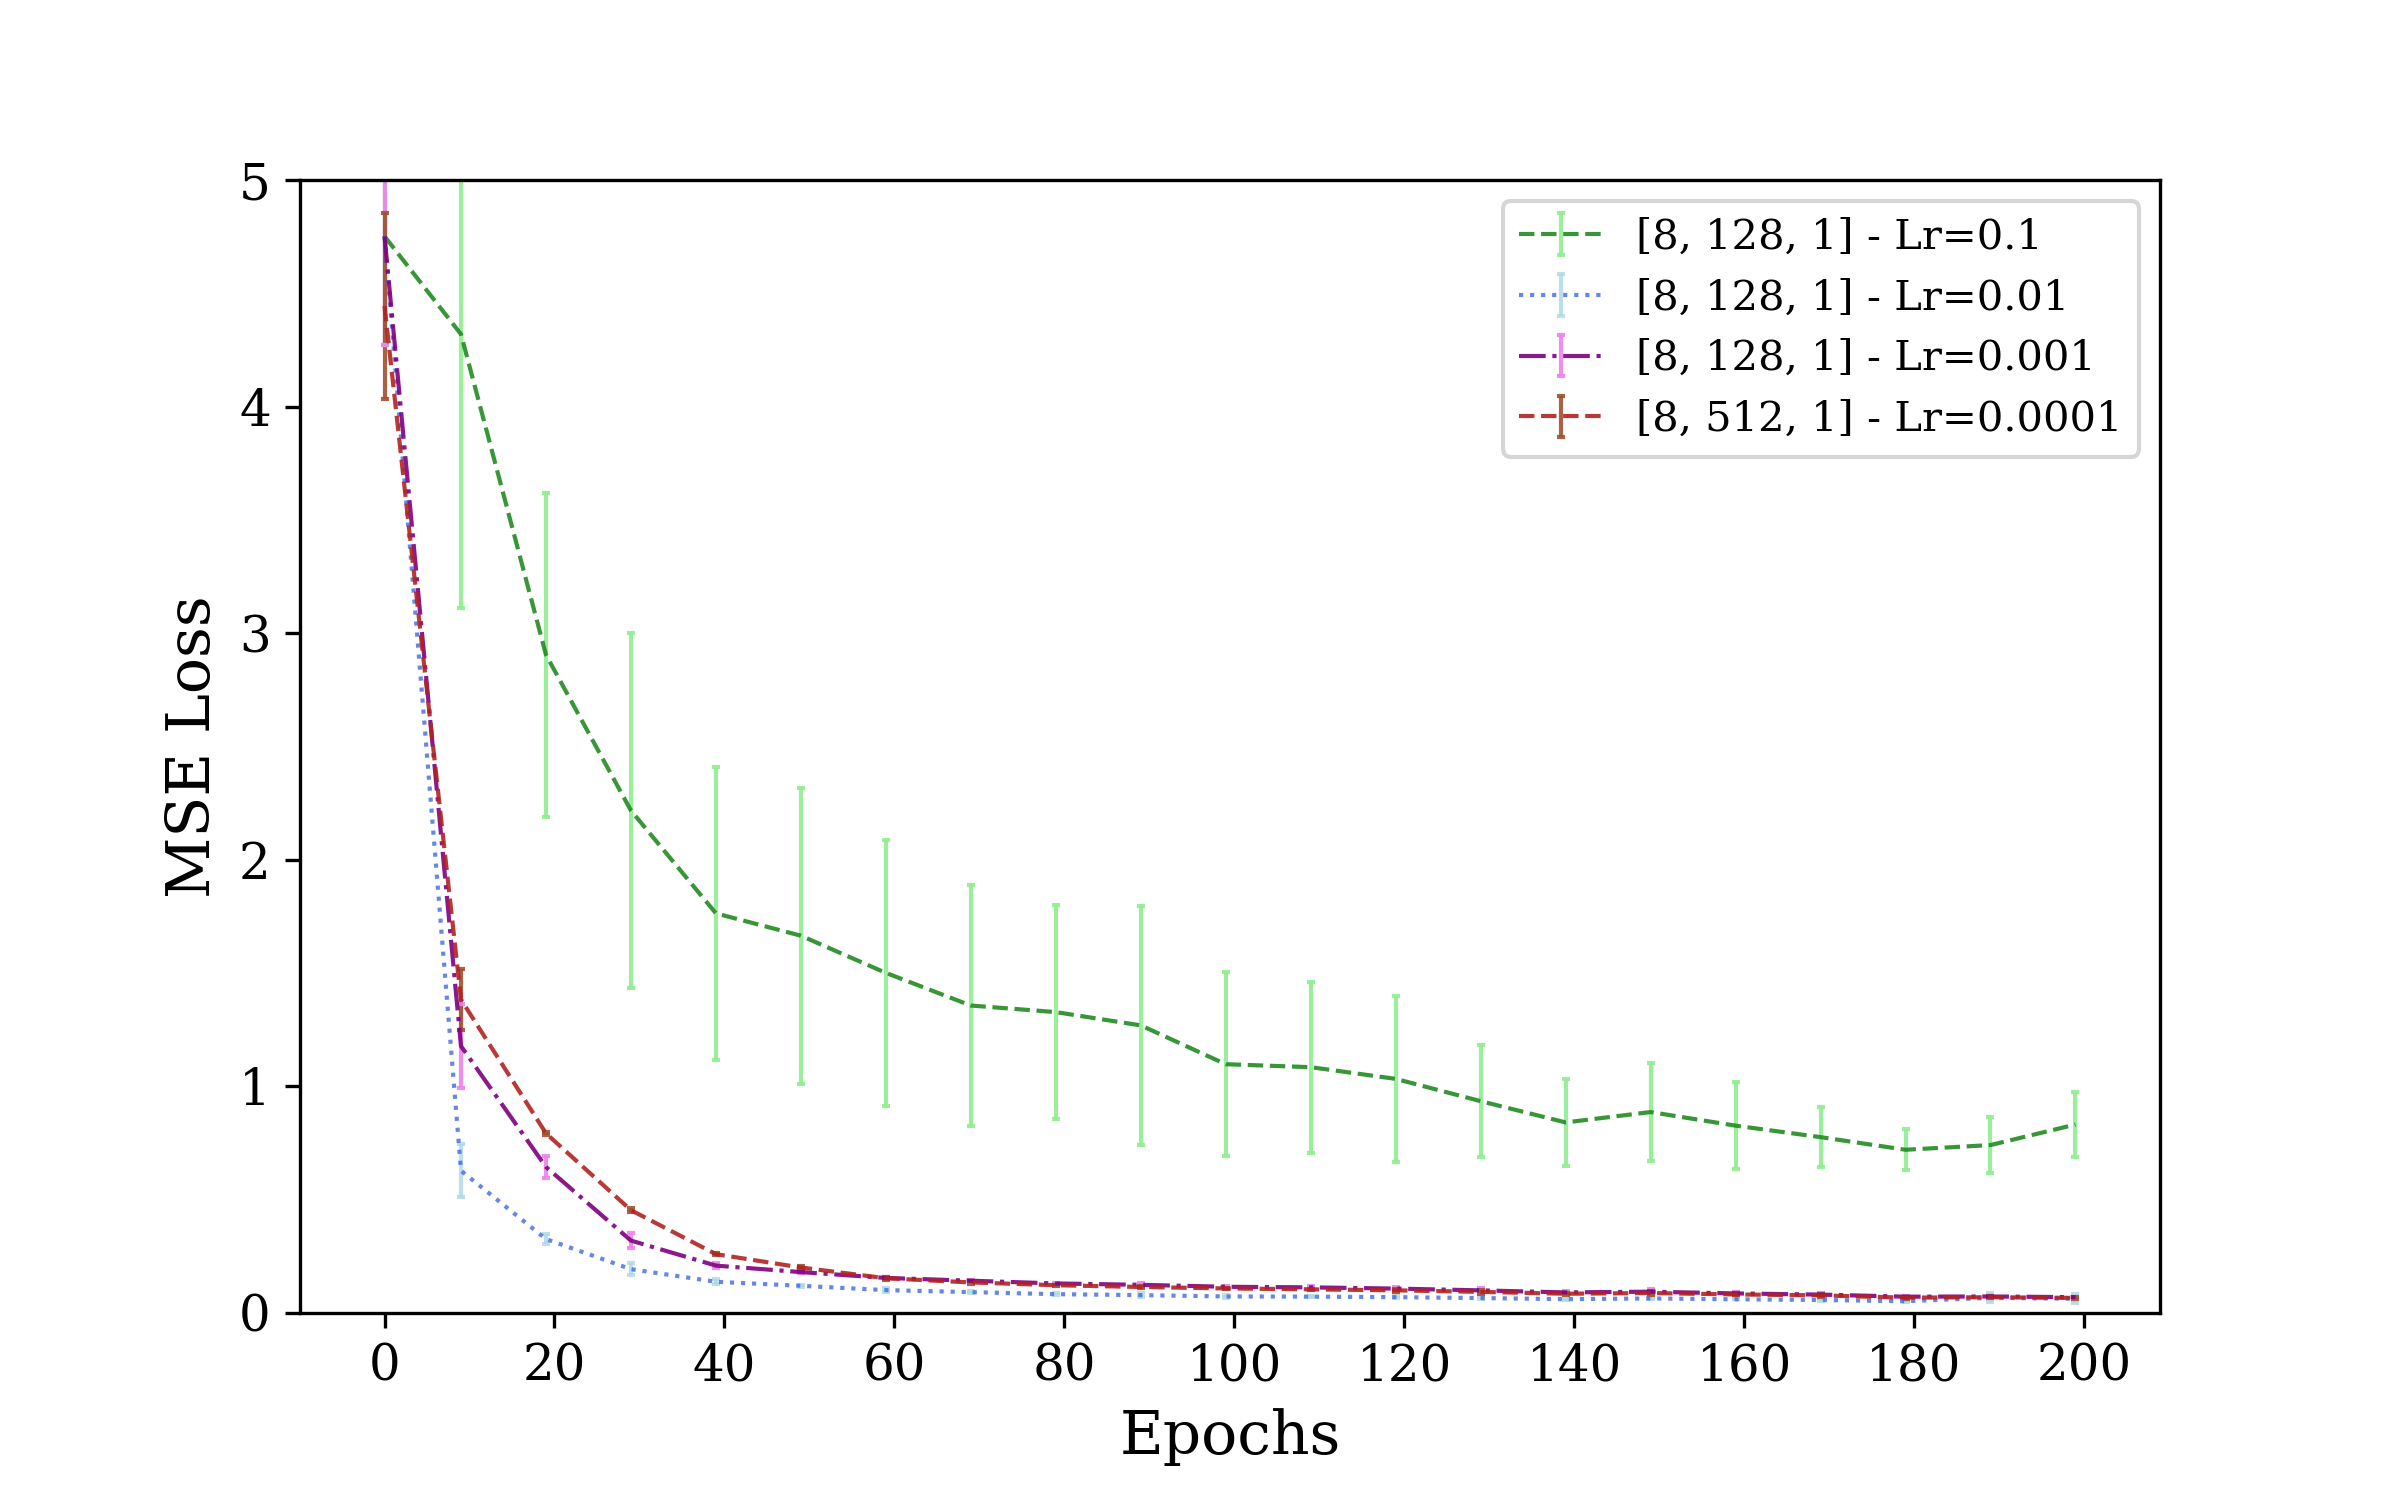
\includegraphics[width=15cm, keepaspectratio]{images/results/module_lr_2.png}
                \caption{MSE Loss Function $L_{pred}$ of the trained modules. The right-hand side number in the legend is the ADAM Learning Rate used for training.}
                \label{fig:results_lr_2}
                
                \vspace{1.5cm}
                
                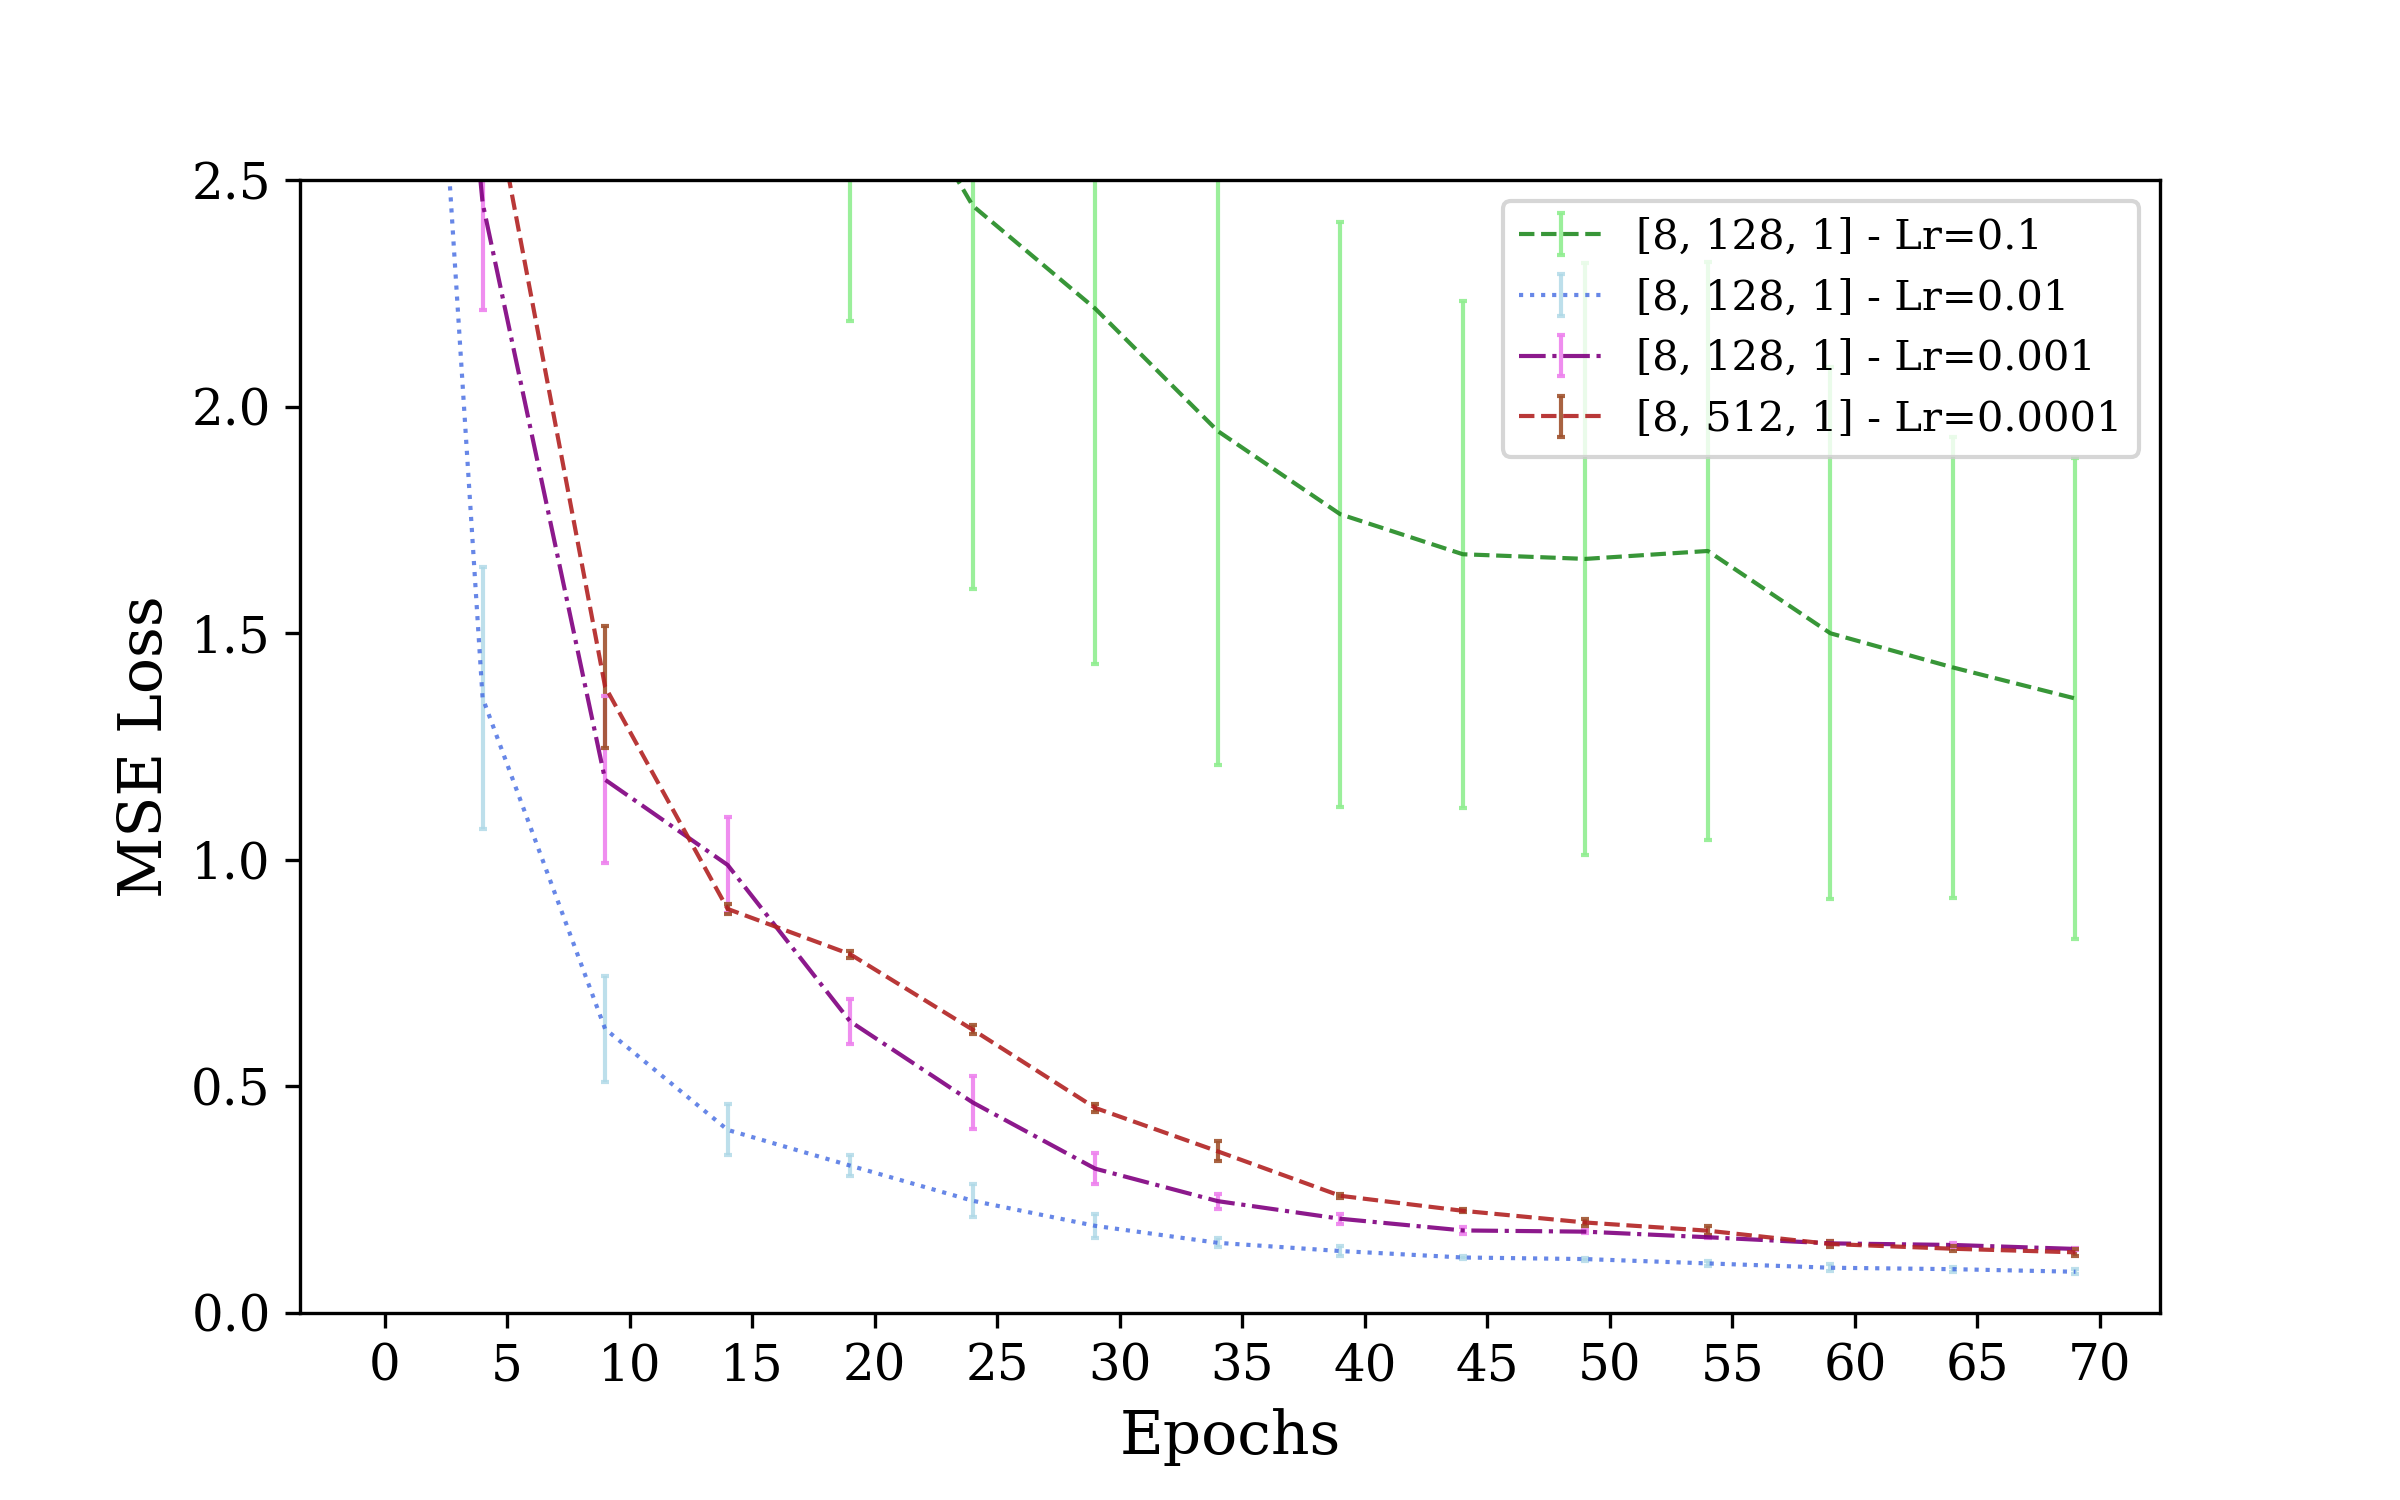
\includegraphics[width=15cm, keepaspectratio]{images/results/module_lr_1.png}
                \caption{MSE Loss Function $L_{pred}$ of the trained modules between Epoch 0 and Epoch 70 for a better illustration. The right-hand side number in the legend is the ADAM Learning Rate used for training.}
                \label{fig:results_lr_1}
        \end{figure}
        
        \begin{figure}[hbtp]
            \centering
            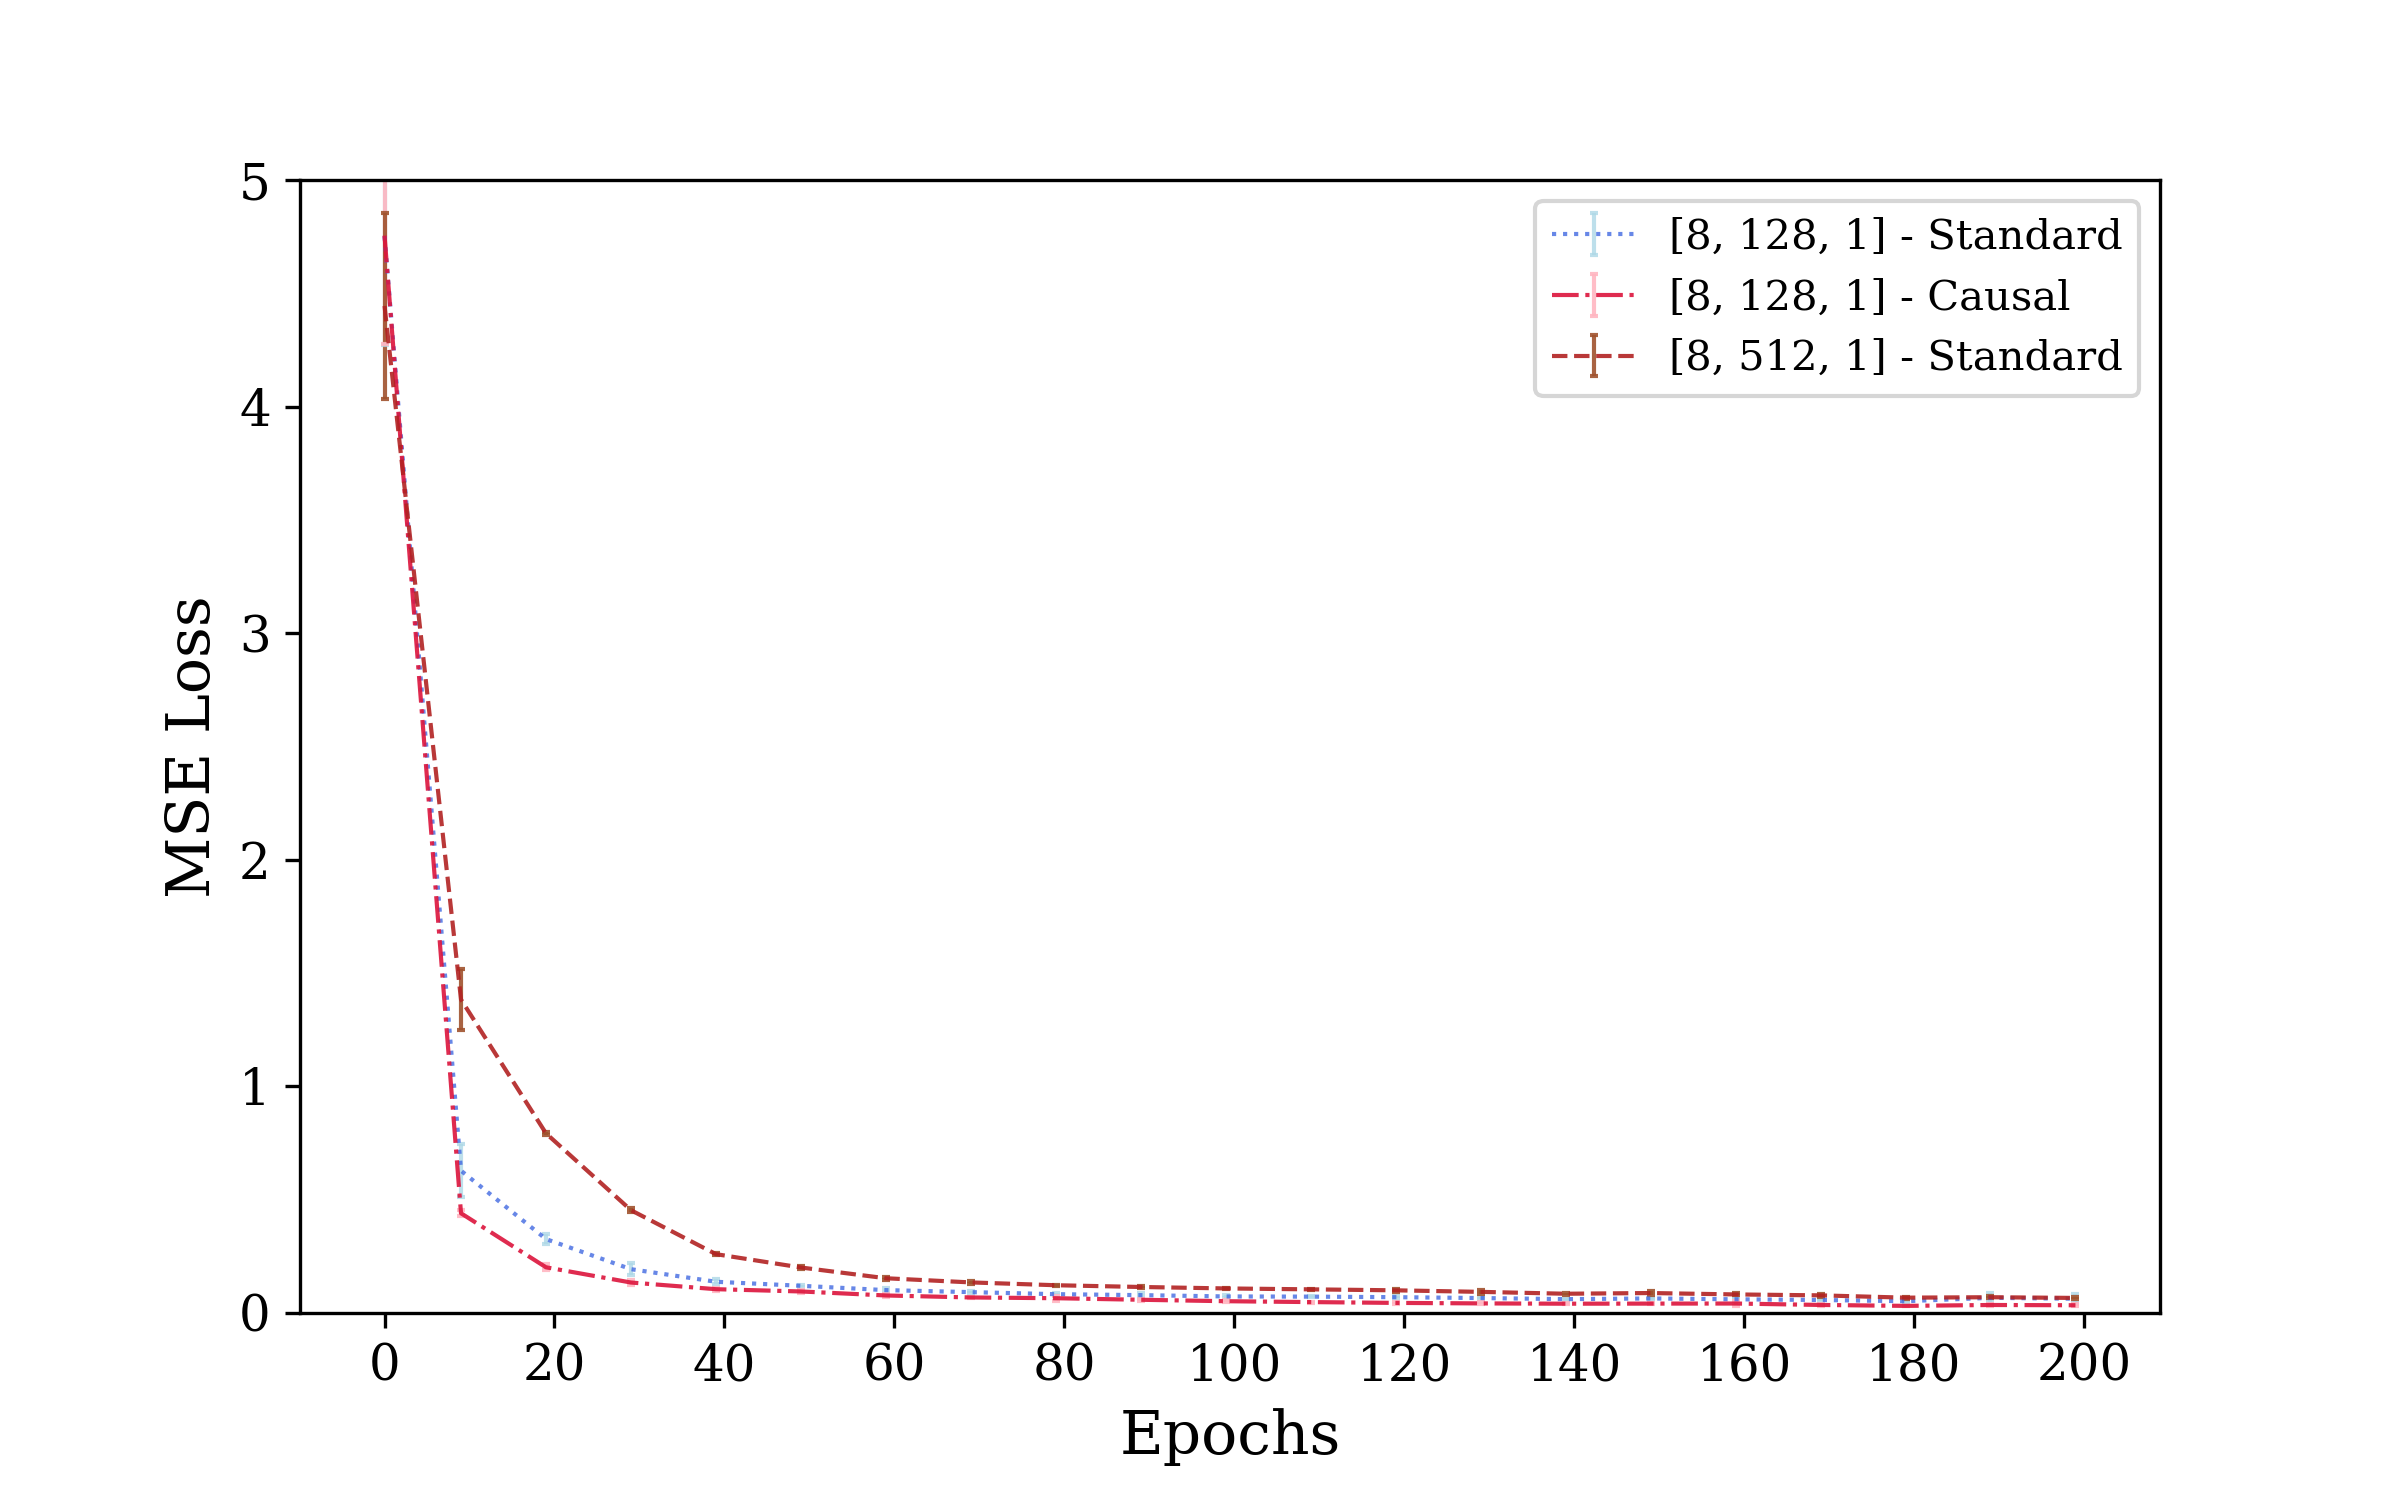
\includegraphics[width=15cm, keepaspectratio]{images/results/module_causal_1.png}
            \caption{MSE Loss Function $L_{pred}$ of the trained modules.}
            \label{fig:results_causal_1}
            
            \vspace{1.5cm}
            
            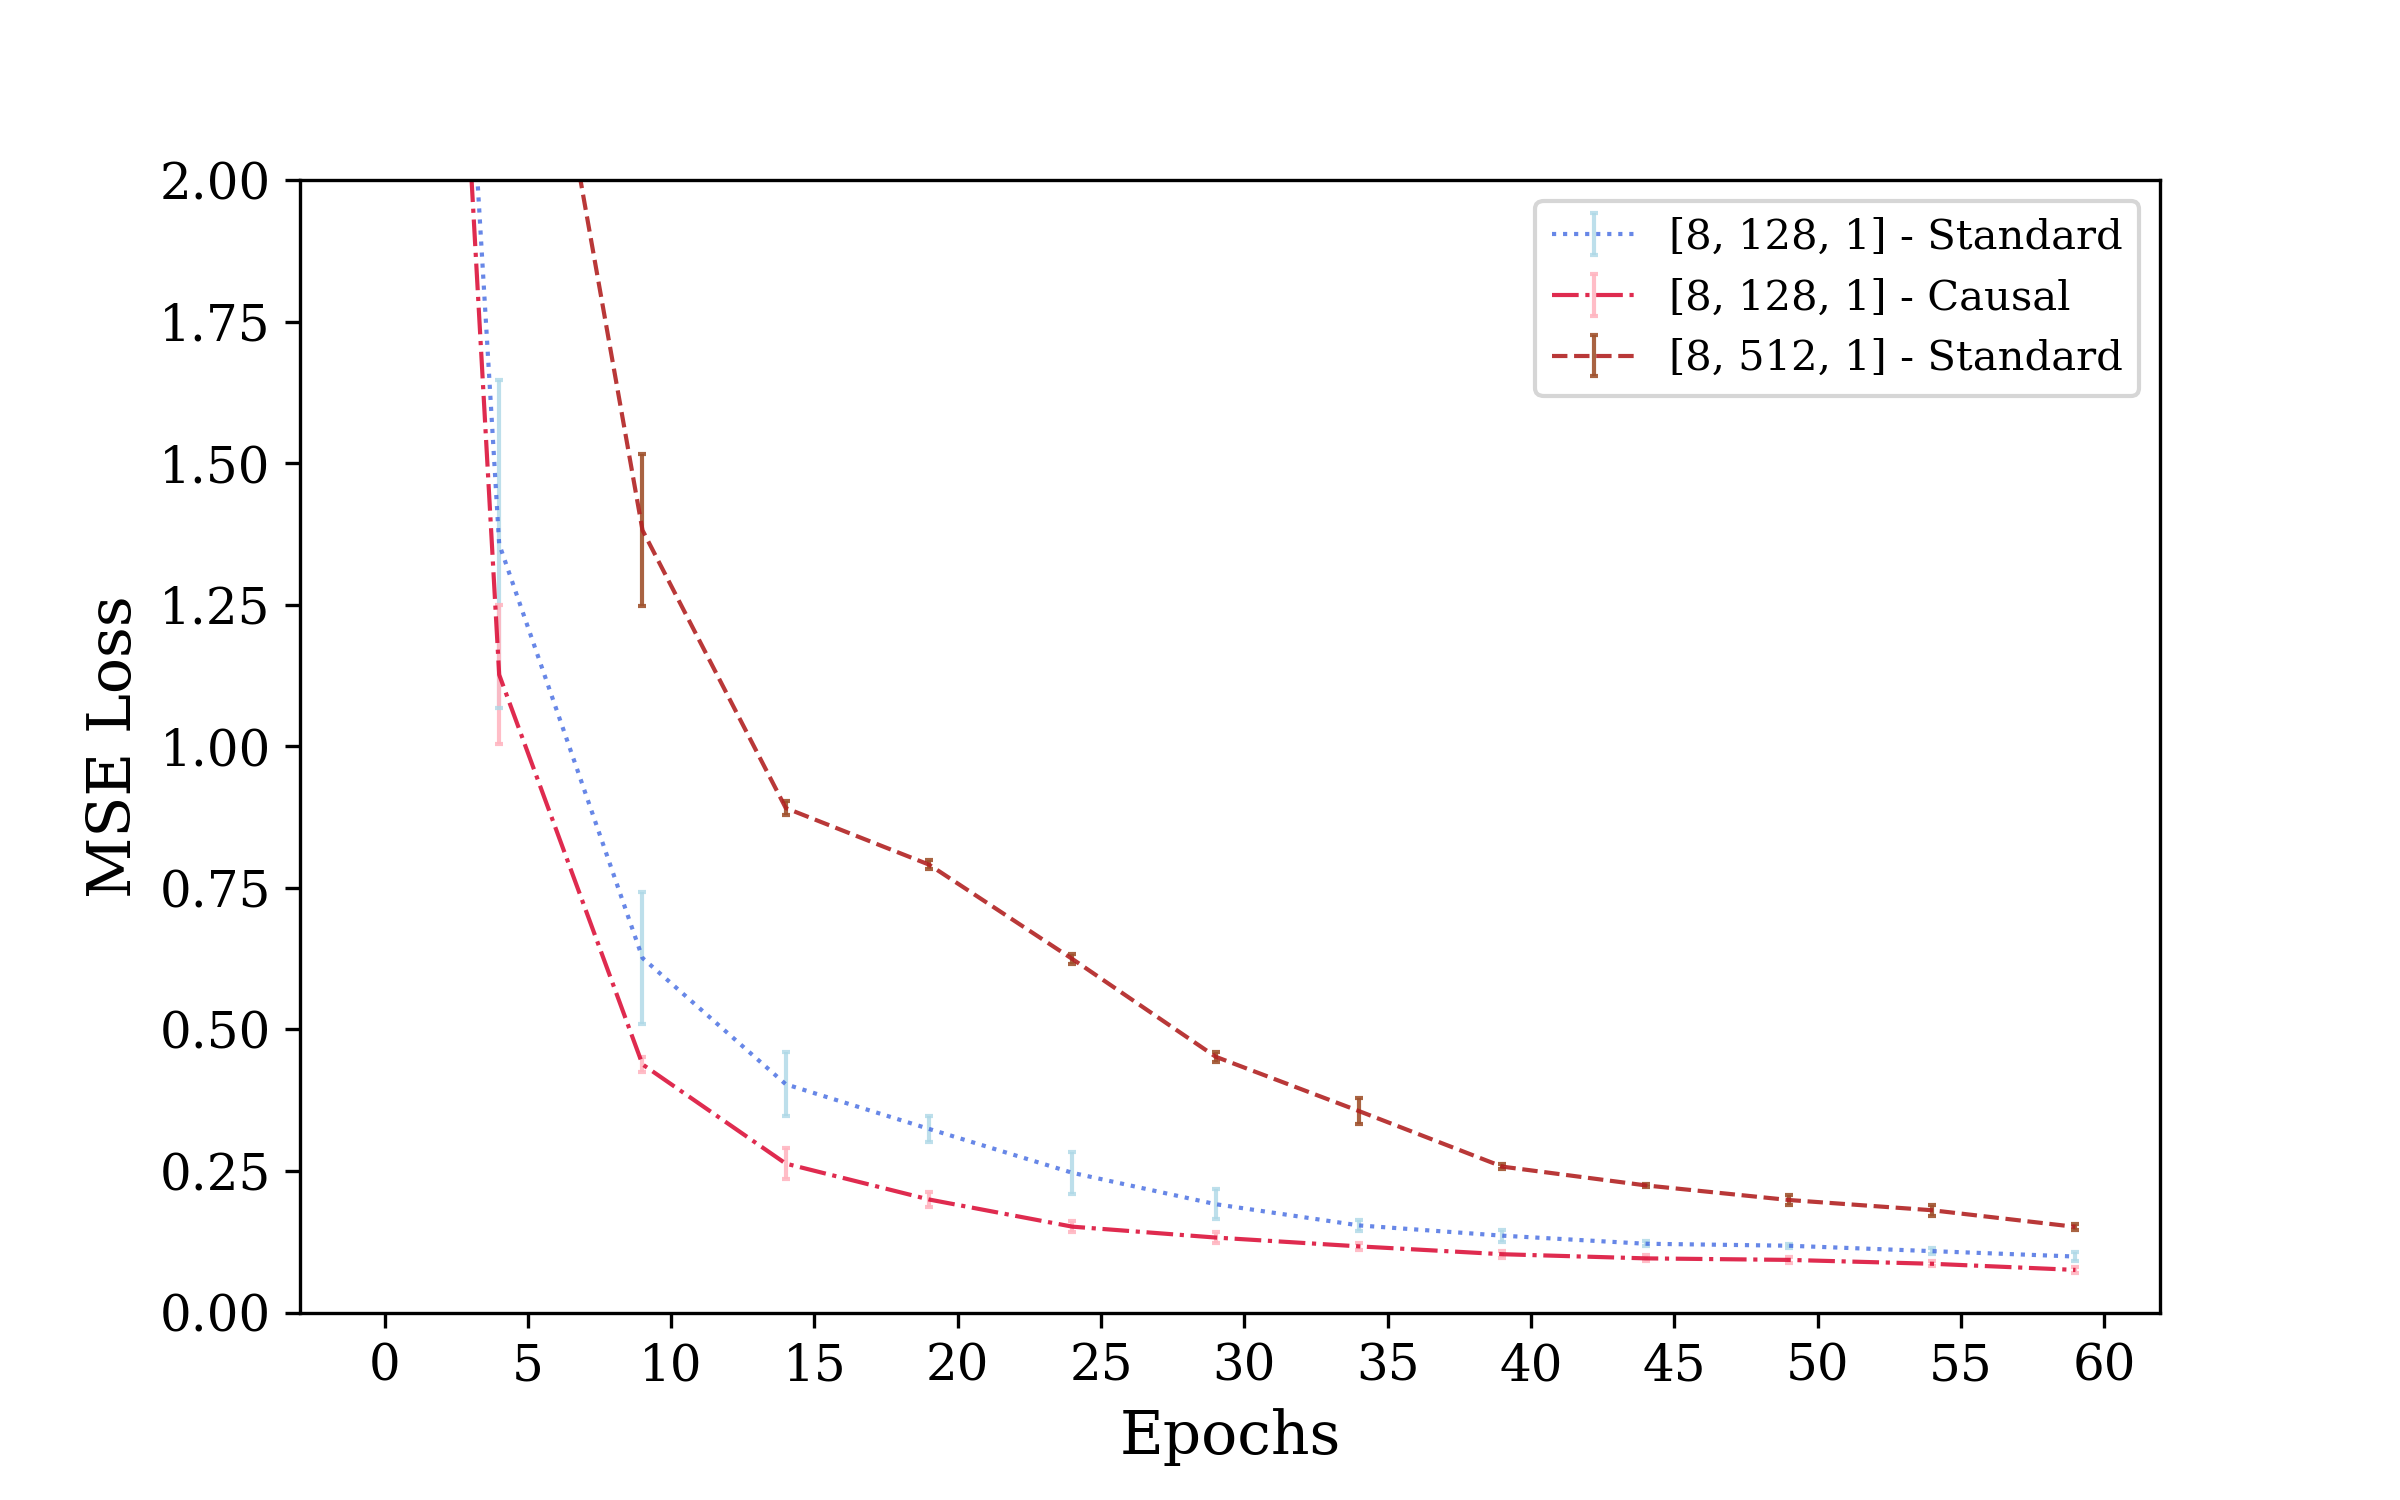
\includegraphics[width=15cm, keepaspectratio]{images/results/module_causal_2.png}
            \caption{MSE Loss Function $L_{pred}$ of the trained modules between Epoch 0 and Epoch 60 for a better illustration.}
            \label{fig:results_causal_2}
        \end{figure}
        
    \newpage
    \section{Deterministic Environment}
    \label{results:deterministic}
    % Inverted Pendulum Results
        This Section is dedicated to results obtained in the deterministic environment Inverted Pendulum. It is divided in two sub-sections: Section \ref{sub:res_det_delays} is concerned with training results obtained by simulated different amount of deterministic and constant delay, while Section \ref{sub:res_stoch_delays} presents training results obtain by simulating the presence of stochastic delays by means of the stochastic process described in Section \ref{sub:simulated_delays}. At the end, the last Section \ref{sub:res_test_delays} discusses the capabilities of the original approach when tested on environments in which the amount of simulated delay is different w.r.t. the one they were trained with. 
        
        \subsection{Deterministic Delays Training Results}
        \label{sub:res_det_delays}
            % SARSA, DSARSA, A-TRPO, M-TRPO, L2-TRPO and D-TRPO Comparison
            All baselines described in Section \ref{sub:baselines}, L2-TRPO and D-TRPO have been trained in the Inverted Pendulum environment. In particular, A-TRPO, M-TRPO and D-TRPO are equipped with policy networks composed of 2 feedforward layers of 64 neurons each and with value function networks composed of 1 feedforward layer of 64 neurons. L2-TRPO has been trained with a policy network composed of 2 feedforward layers of 67 neurons each and with a value function network with 1 feedforward layer of 128 neurons. D-TRPO and L2-TRPO have been deployed respectively with a [8, 64, 1] and a [8, 68, 1] modules, according to the notation presented in Section \ref{results:module_tuning}. L2-TRPO parameters have been slightly enlarged so that the entire network has a similar total number of parameters to D-TRPO, which is also equipped with a MAF network. All algorithms have been trained for 2000 epochs, each composed of 5000 steps for a total of 10 millions steps. Each trajectory in the environment lasts for 250 steps. Each algorithm has been trained with different amounts of deterministic and constant simulated delay, specifically we chose to test 3, 5, 10 and 15 time-steps of delay. At last, TRPO has beed trained on the same context without delays as a reference for the best possible performance it is possible to obtain.
            
            \subsubsection{Results Description}
                We start discussing the results from the 3-steps delay and then increasing delay. As figure \ref{fig:results_delay3_1} shows, D-TRPO, L2-TRPO and M-TRPO are able to cope with 3 steps of delay without particular issues: even if M-TRPO is slightly slower than the other two, all of them are able to reach undelayed TRPO's average reward, albeit slower. Instead, A-TRPO is already greatly affected by the state augmentation and it does not manage to converge towards the optimal behaviour. At the same time, both SARSA and D-SARSA converge to a slightly better performance than A-TRPO, while still being substantially affected by the delay.\newline
                Training with 5 steps of delays shows similar results: as expected, each algorithm is affected by the larger delay with slower convergence and/or slower final average reward. The main observable difference is the loss of performances that M-TRPO shows, without being able to reach the same level of performances of undelayed TRPO.\newline
                A delay of 10 time-step heavily affects even L2-TRPO and D-TRPO, which are still able to outperform the other algorithms, but they no longer match undelayed TRPO performances. At the end, 15 steps of delay proves to be too large for any algorithm to show a significant performance improvement, with M-TRPO reaching the best result overall.
            
            \subsubsection{Result Discussion}
                This set of training procedures shows that the proposed approach is solid and able to produce promising results. Both D-TRPO and L2-TRPO are able to outperform almost any other baselines, regardless the amount of delay present, even matching undelayed TRPO performances for lower delays, effectivaly nullfying the presence of delays. However, it is also interesting to note that M-TRPO is also able to keep up throughout the tests and it proves to be more resilient that other algorithms to large delays, possibly suggesting that it could be the preferred method in some range of delays. 
            
            \begin{figure}[hbtp]
                \centering
                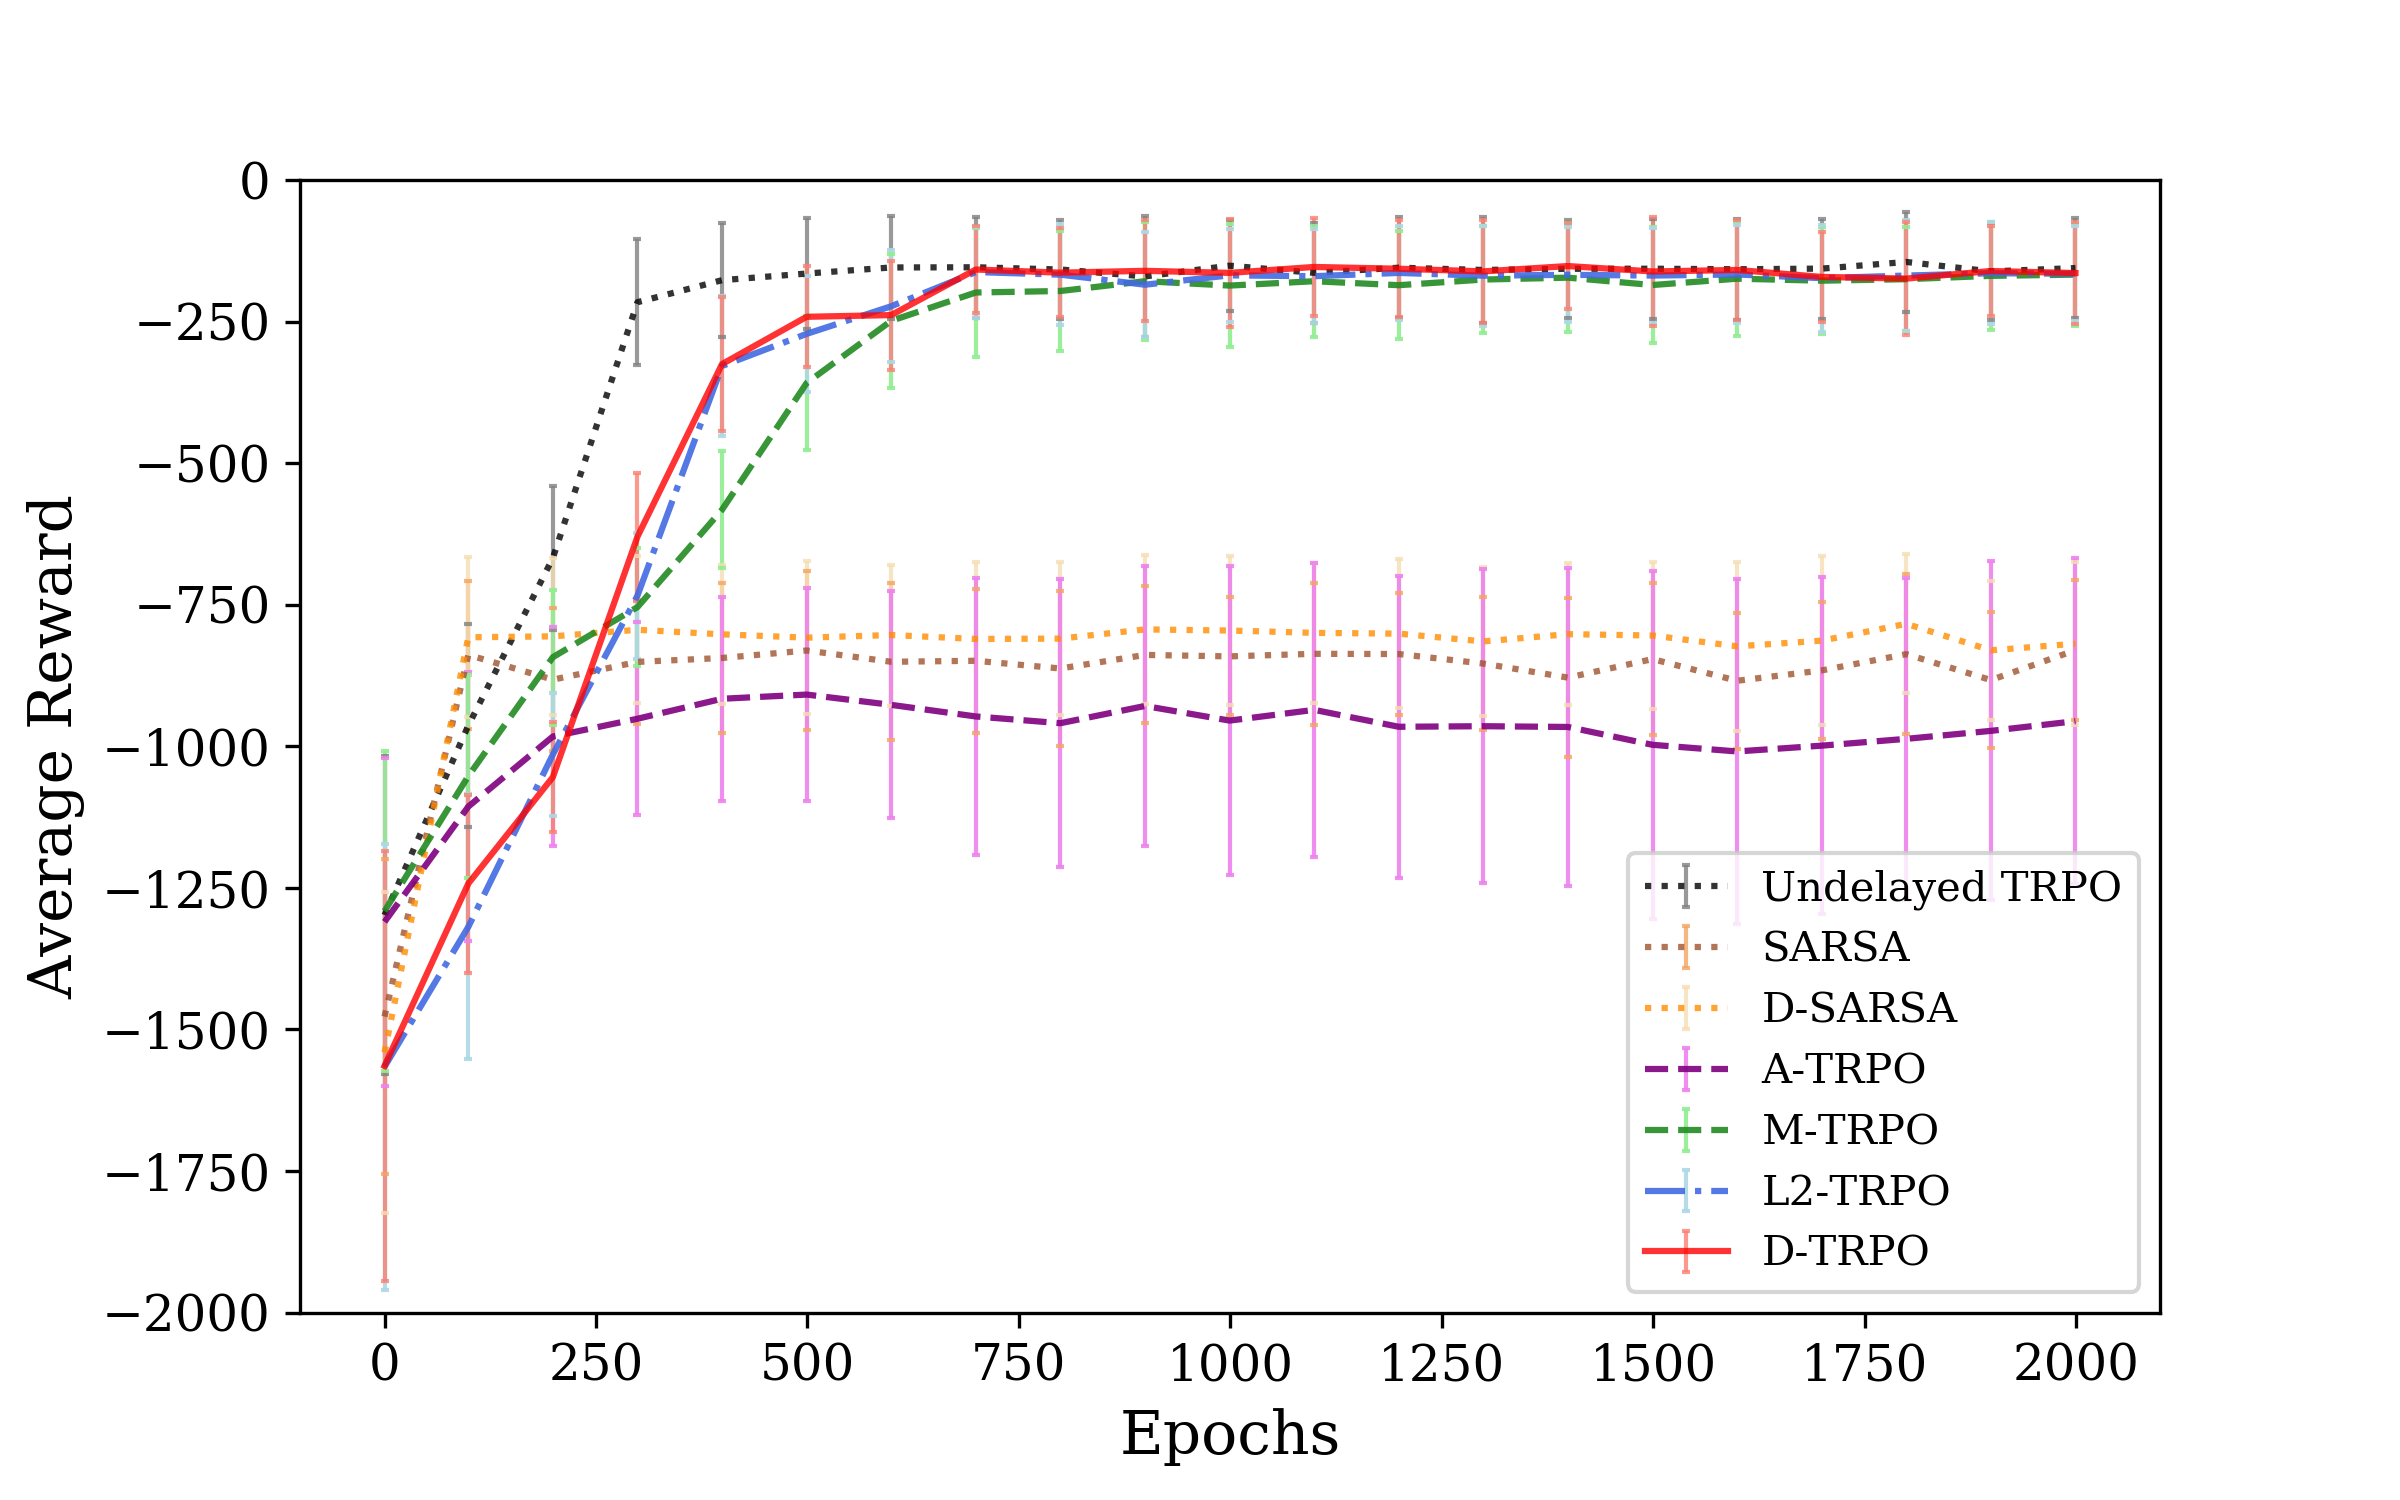
\includegraphics[width=15cm, keepaspectratio]{images/results/delay3_comparisons_1.png}
                \caption{Training results obtained in a 3-steps delay and deterministic environment setting.}
                \label{fig:results_delay3_1}
                
                \vspace{1.5cm}
                
                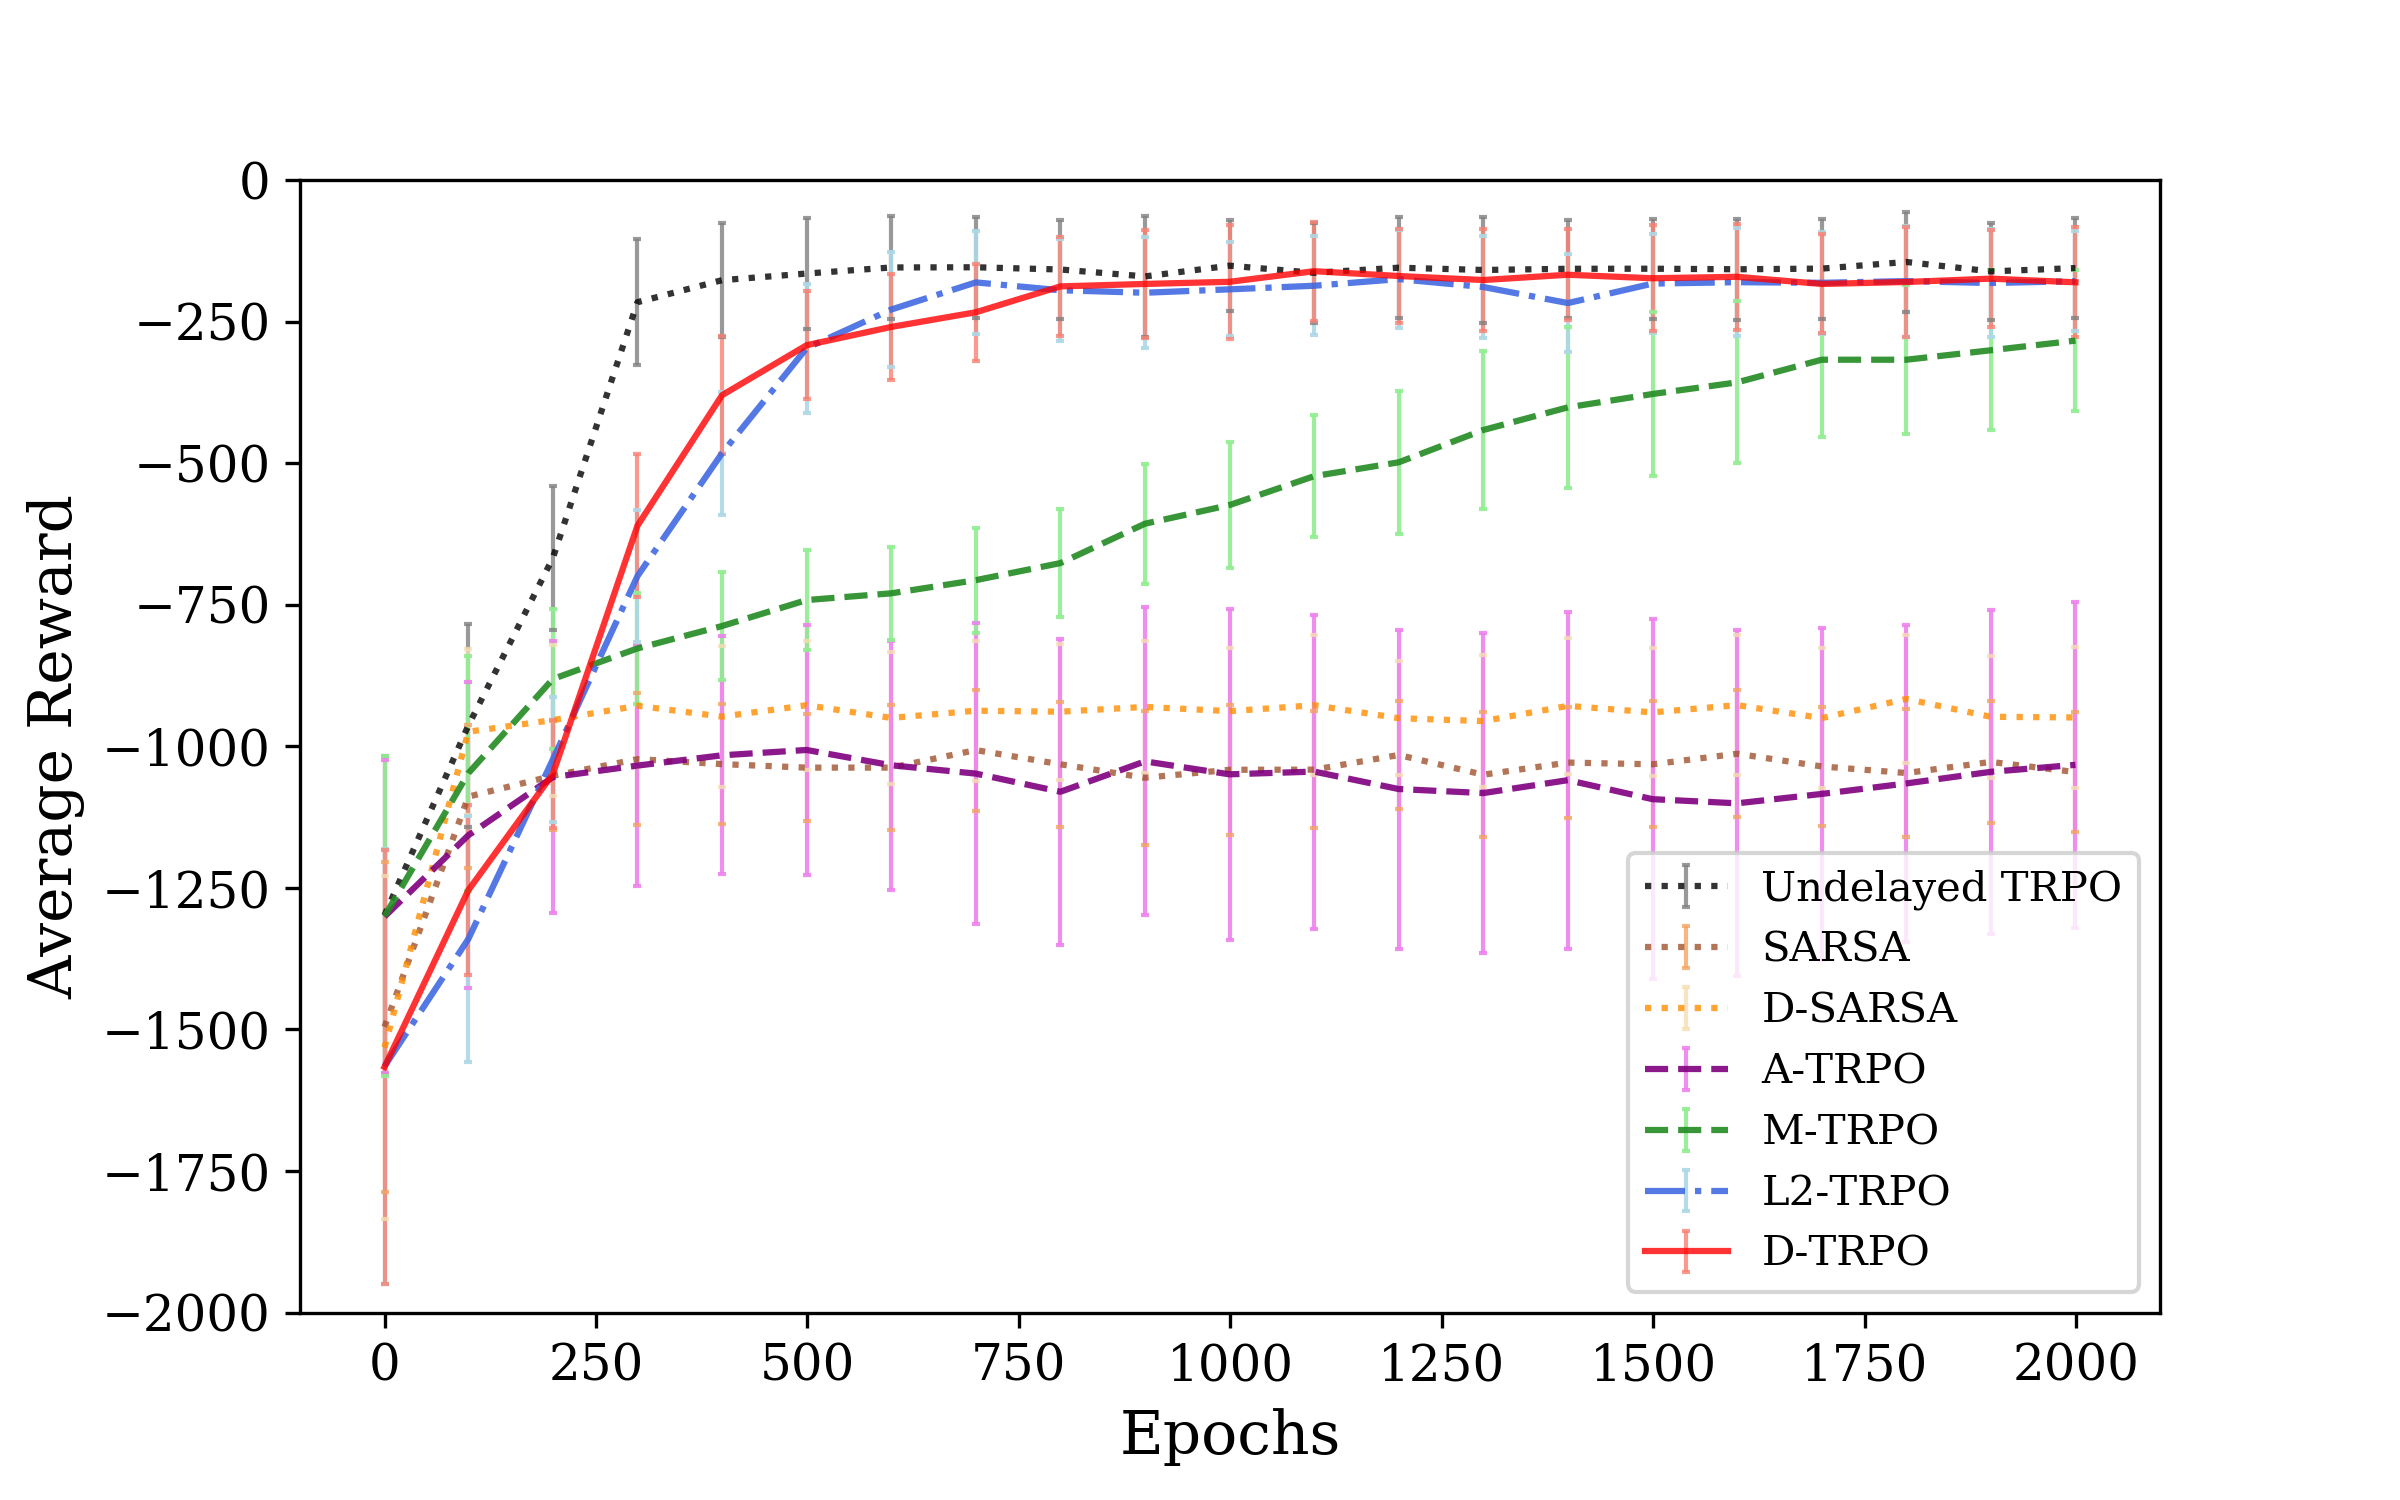
\includegraphics[width=15cm, keepaspectratio]{images/results/delay5_comparisons_1.png}
                \caption{Training results obtained in a 5-steps delay and deterministic environment setting.}
                \label{fig:results_delay5_1}
            \end{figure}
            
            \begin{figure}[hbtp]
                \centering
                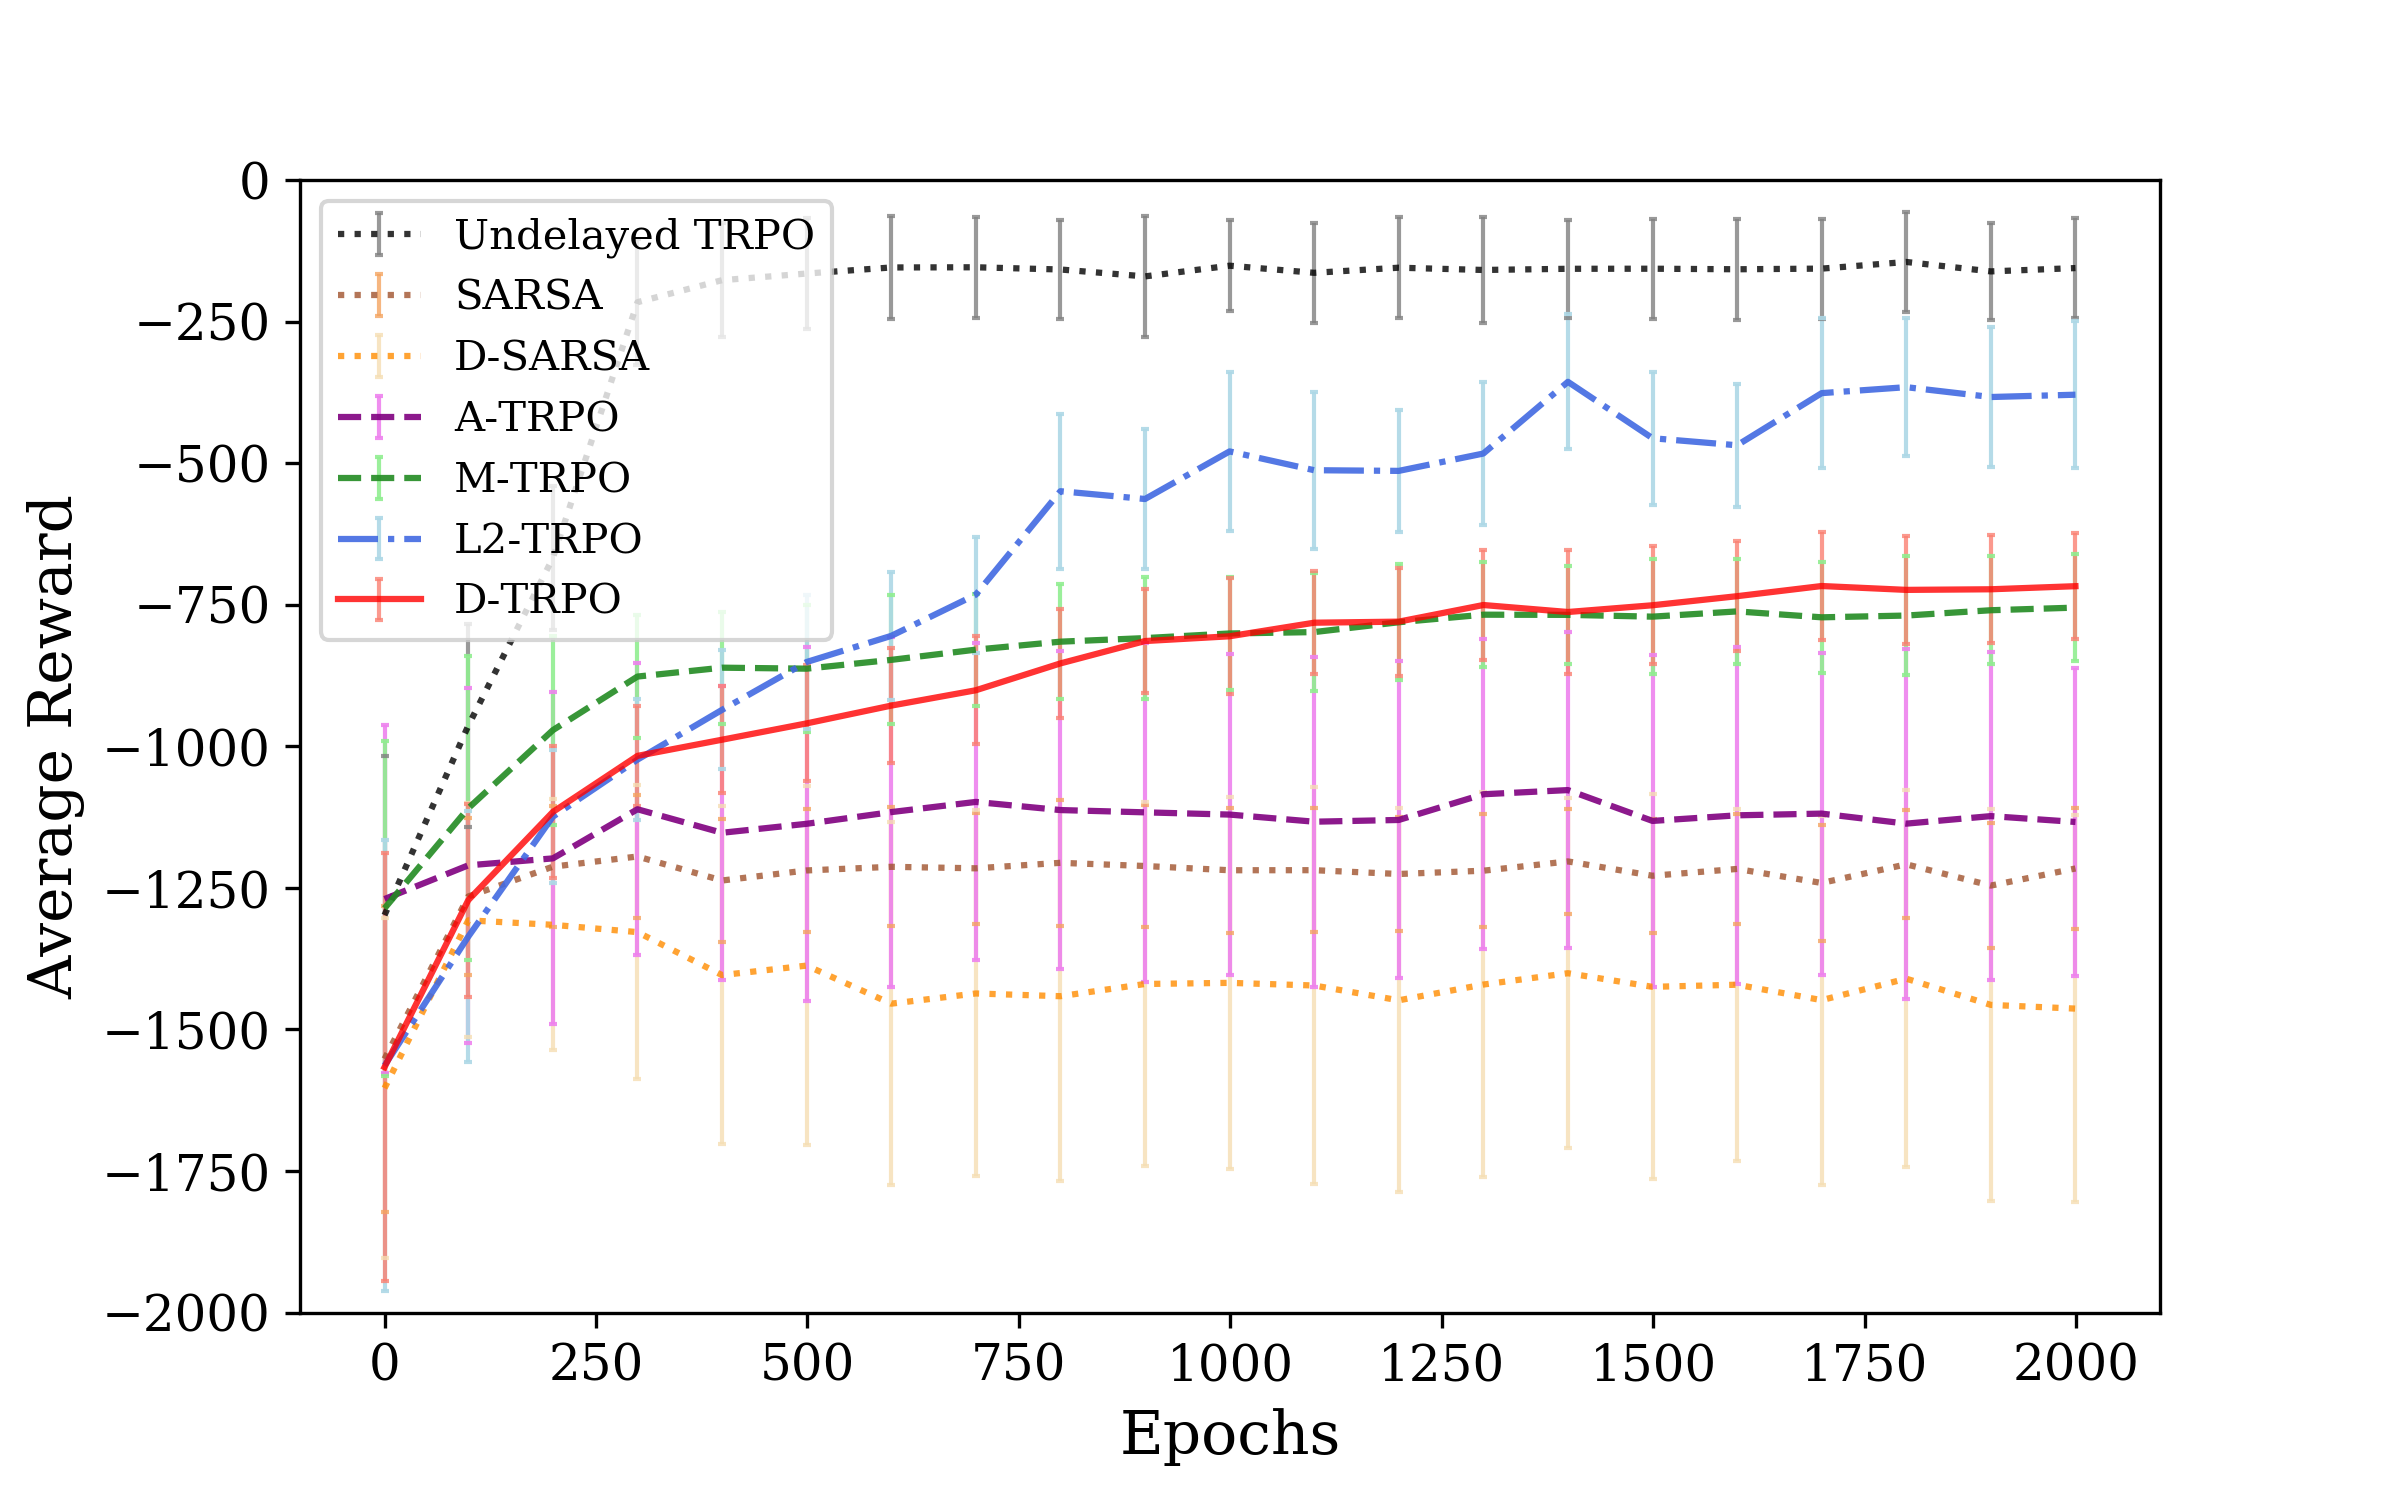
\includegraphics[width=15cm, keepaspectratio]{images/results/delay10_comparisons_1.png}
                \caption{Training results obtained in a 10-steps delay and deterministic environment setting.}
                \label{fig:results_delay10_1}
                
                \vspace{1.5cm}
                
                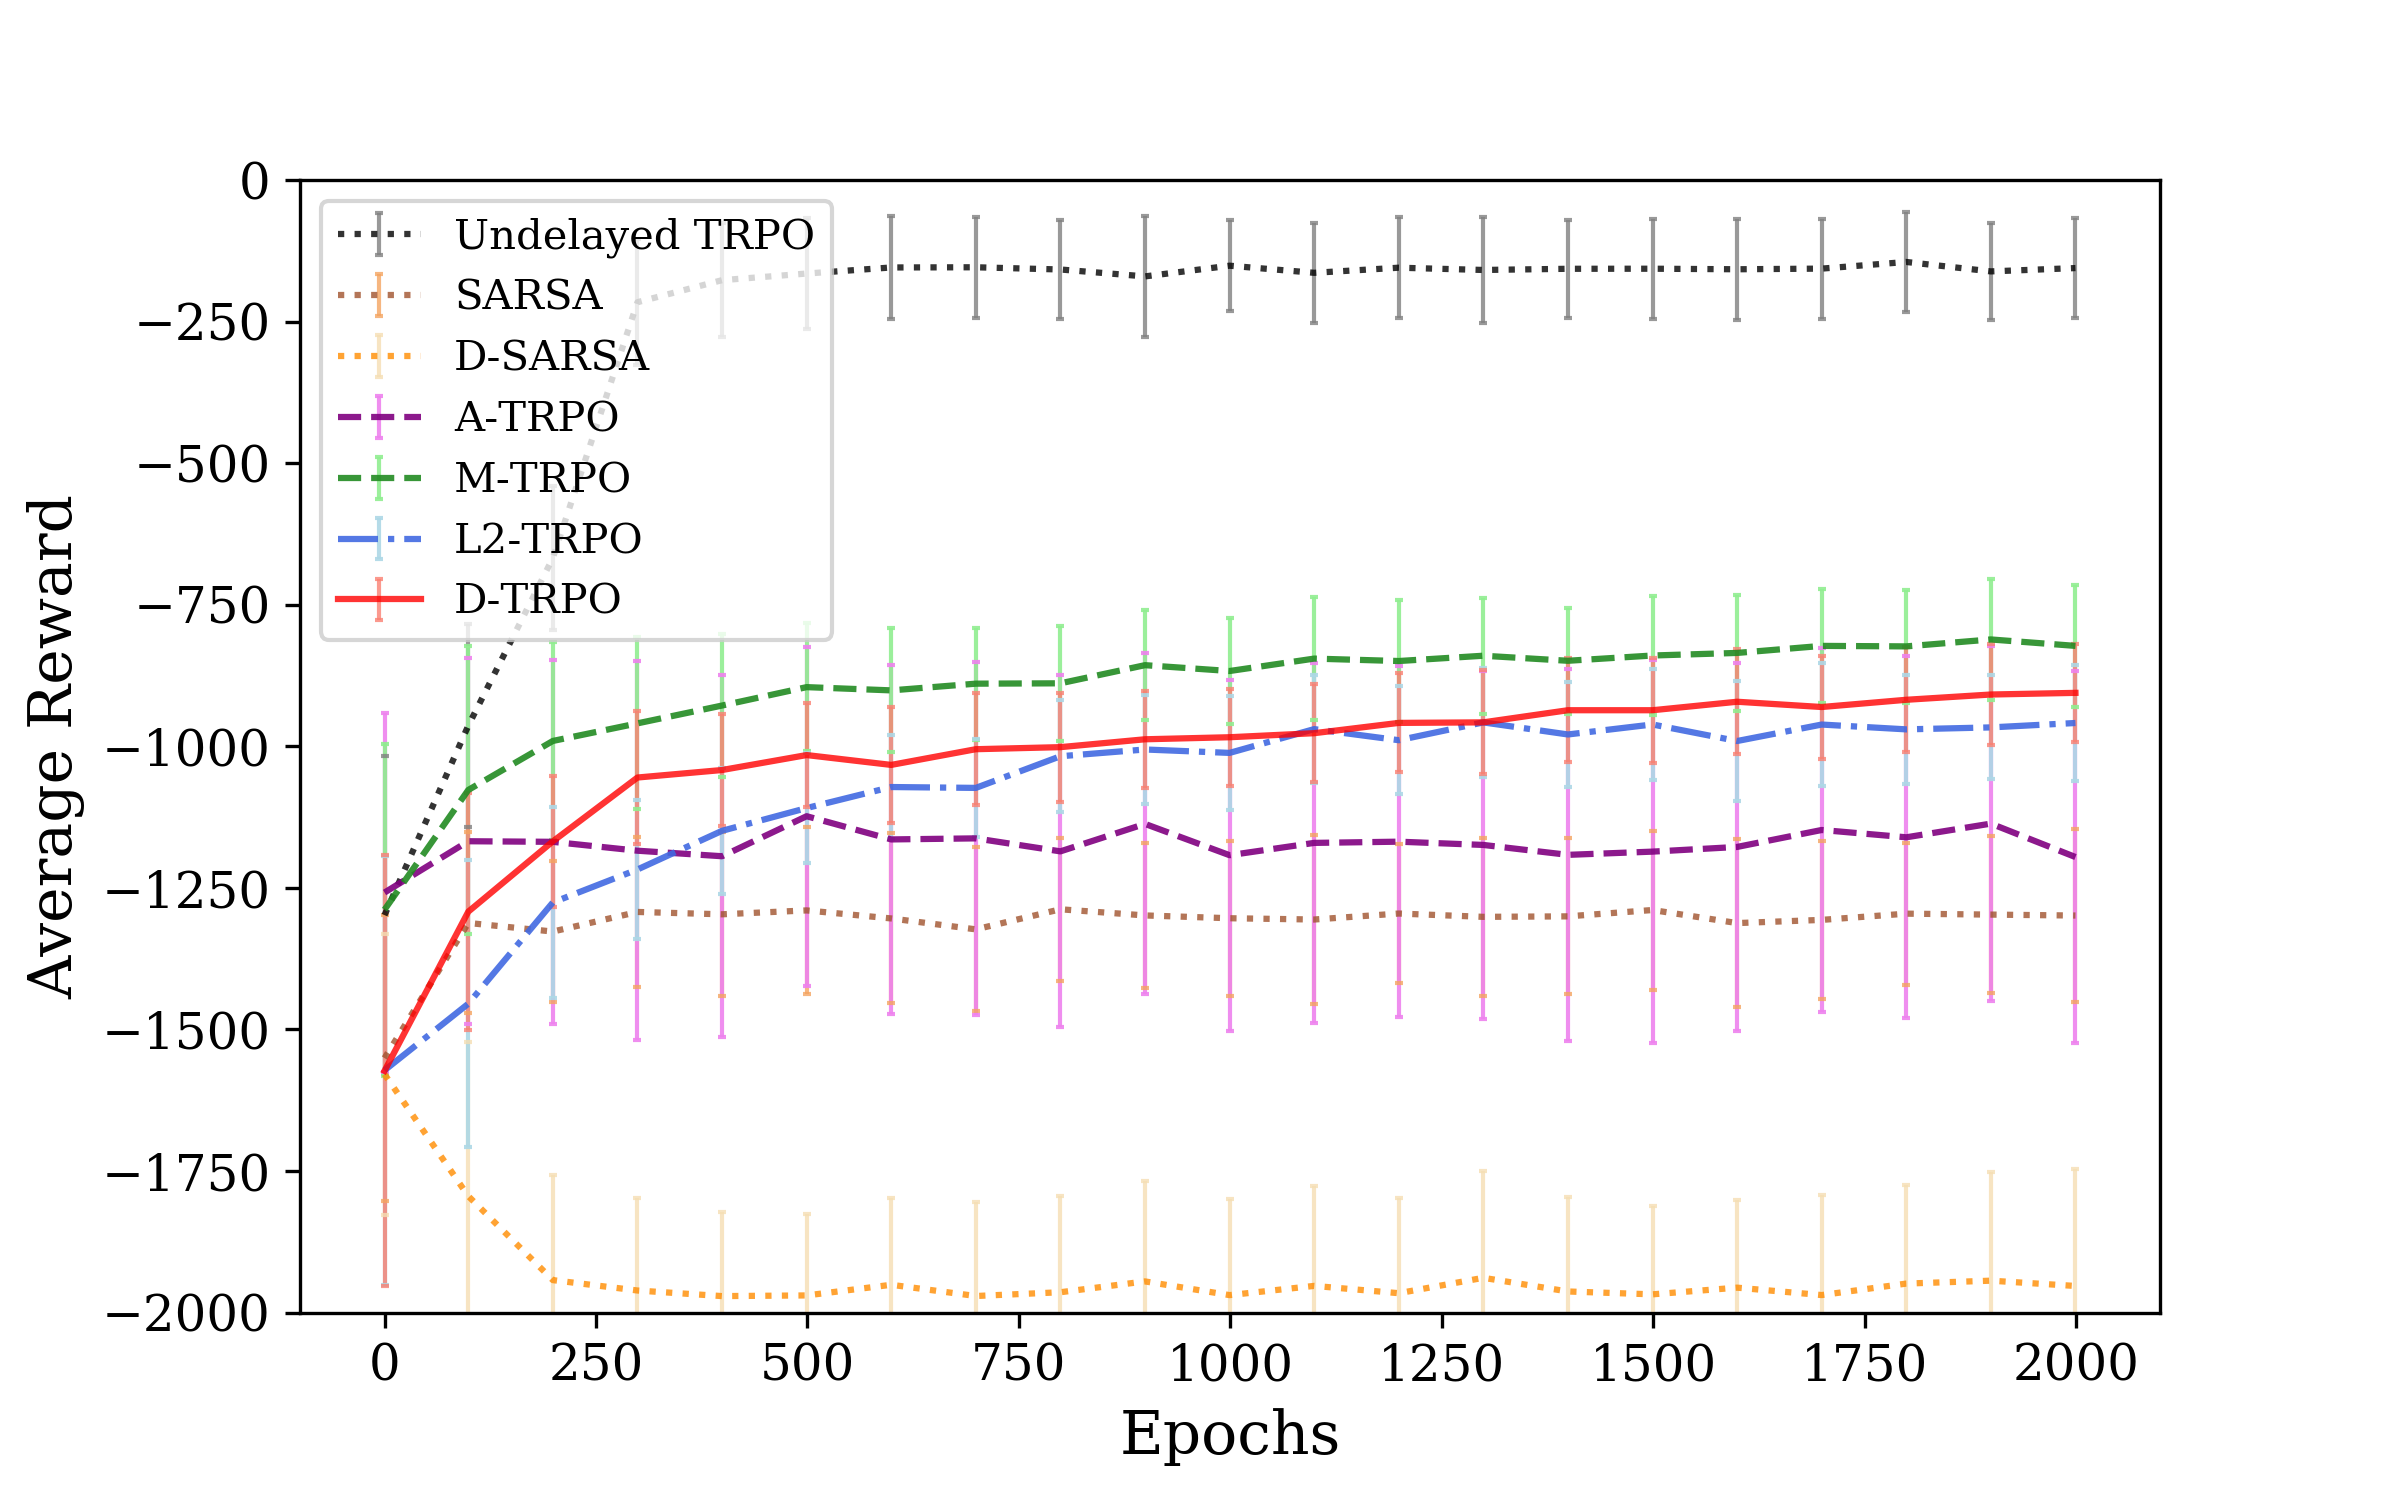
\includegraphics[width=15cm, keepaspectratio]{images/results/delay15_comparisons_1.png}
                \caption{Training results obtained in a 15-steps delay and deterministic environment setting.}
                \label{fig:results_delay15_1}
            \end{figure}
        
        \newpage
        \subsection{Stochastic Delays Training Results}
        \label{sub:res_stoch_delays}
            % Only D-TRPO and L2-TRPO can natively handle them (Attention Network)
            % D-TRPO Tests --> Bad Results, keep training on Deterministic
            % Compare the trained model on Stochastic Delays against the Min/Max Deterministic Delay
            We decided to test D-TRPO in a stochastic delay context, deploying the same settings for the networks as in the previous test. We train D-TRPO for 500 epochs composed of 5000 steps each, while each trajectory in the environment lasts for 250 steps, and simulating three different stochastic delay processes respectively with $p=0.7$, $p=0.6$ and $p=0.55$.
            \\\\
            Figures \ref{fig:results_delayp07_1}, \ref{fig:results_delayp06_1} and \ref{fig:results_delayp05_1} illustrates the resulting training process, comparing them to D-TRPO and L2-TRPO trained with a constant delay closest to the average delay of each stochastic process, also shown in Figures \ref{fig:delayp07_sampledelay}, \ref{fig:delayp06_sampledelay} and \ref{fig:delayp05_sampledelay} respectively. Unfortunately, results are underwhelming compared with similar deterministic delays. Starting from $p=0.7$, which is compared to 3 steps of delays, D-TRPO shows an inconsistent learning process that converges to a lower average reward, even decreasing w.r.t. its peak performances. Stochastic delays with $p=0.6$ is compared to 5 steps of delays and it shows a similar behaviour to $p=0.7$, while $p=0.5$ is compared with 10 steps of delay and shows very kin performances at 500 epochs, nevertheless D-TRPO with stochastic delays has already converged.
            The reason behind inconsistent performances may be related to the higher variance the stochastic delay process induces in the input data, the extended states. While in deterministic delays we expect the extended state to have a fixed size and, consequently, the module to predict the same number of steps at each time-step, stochastic delays disrupt this process: the extended state has different sizes and the same set of parameter must be able to predict for a different number of time steps. Thus, the module needs to be able to deal not only with all possible combinations of states and sequence of actions in the extended state, but also with all possible sizes of the extended state. 
            
            \begin{figure}[!b]
                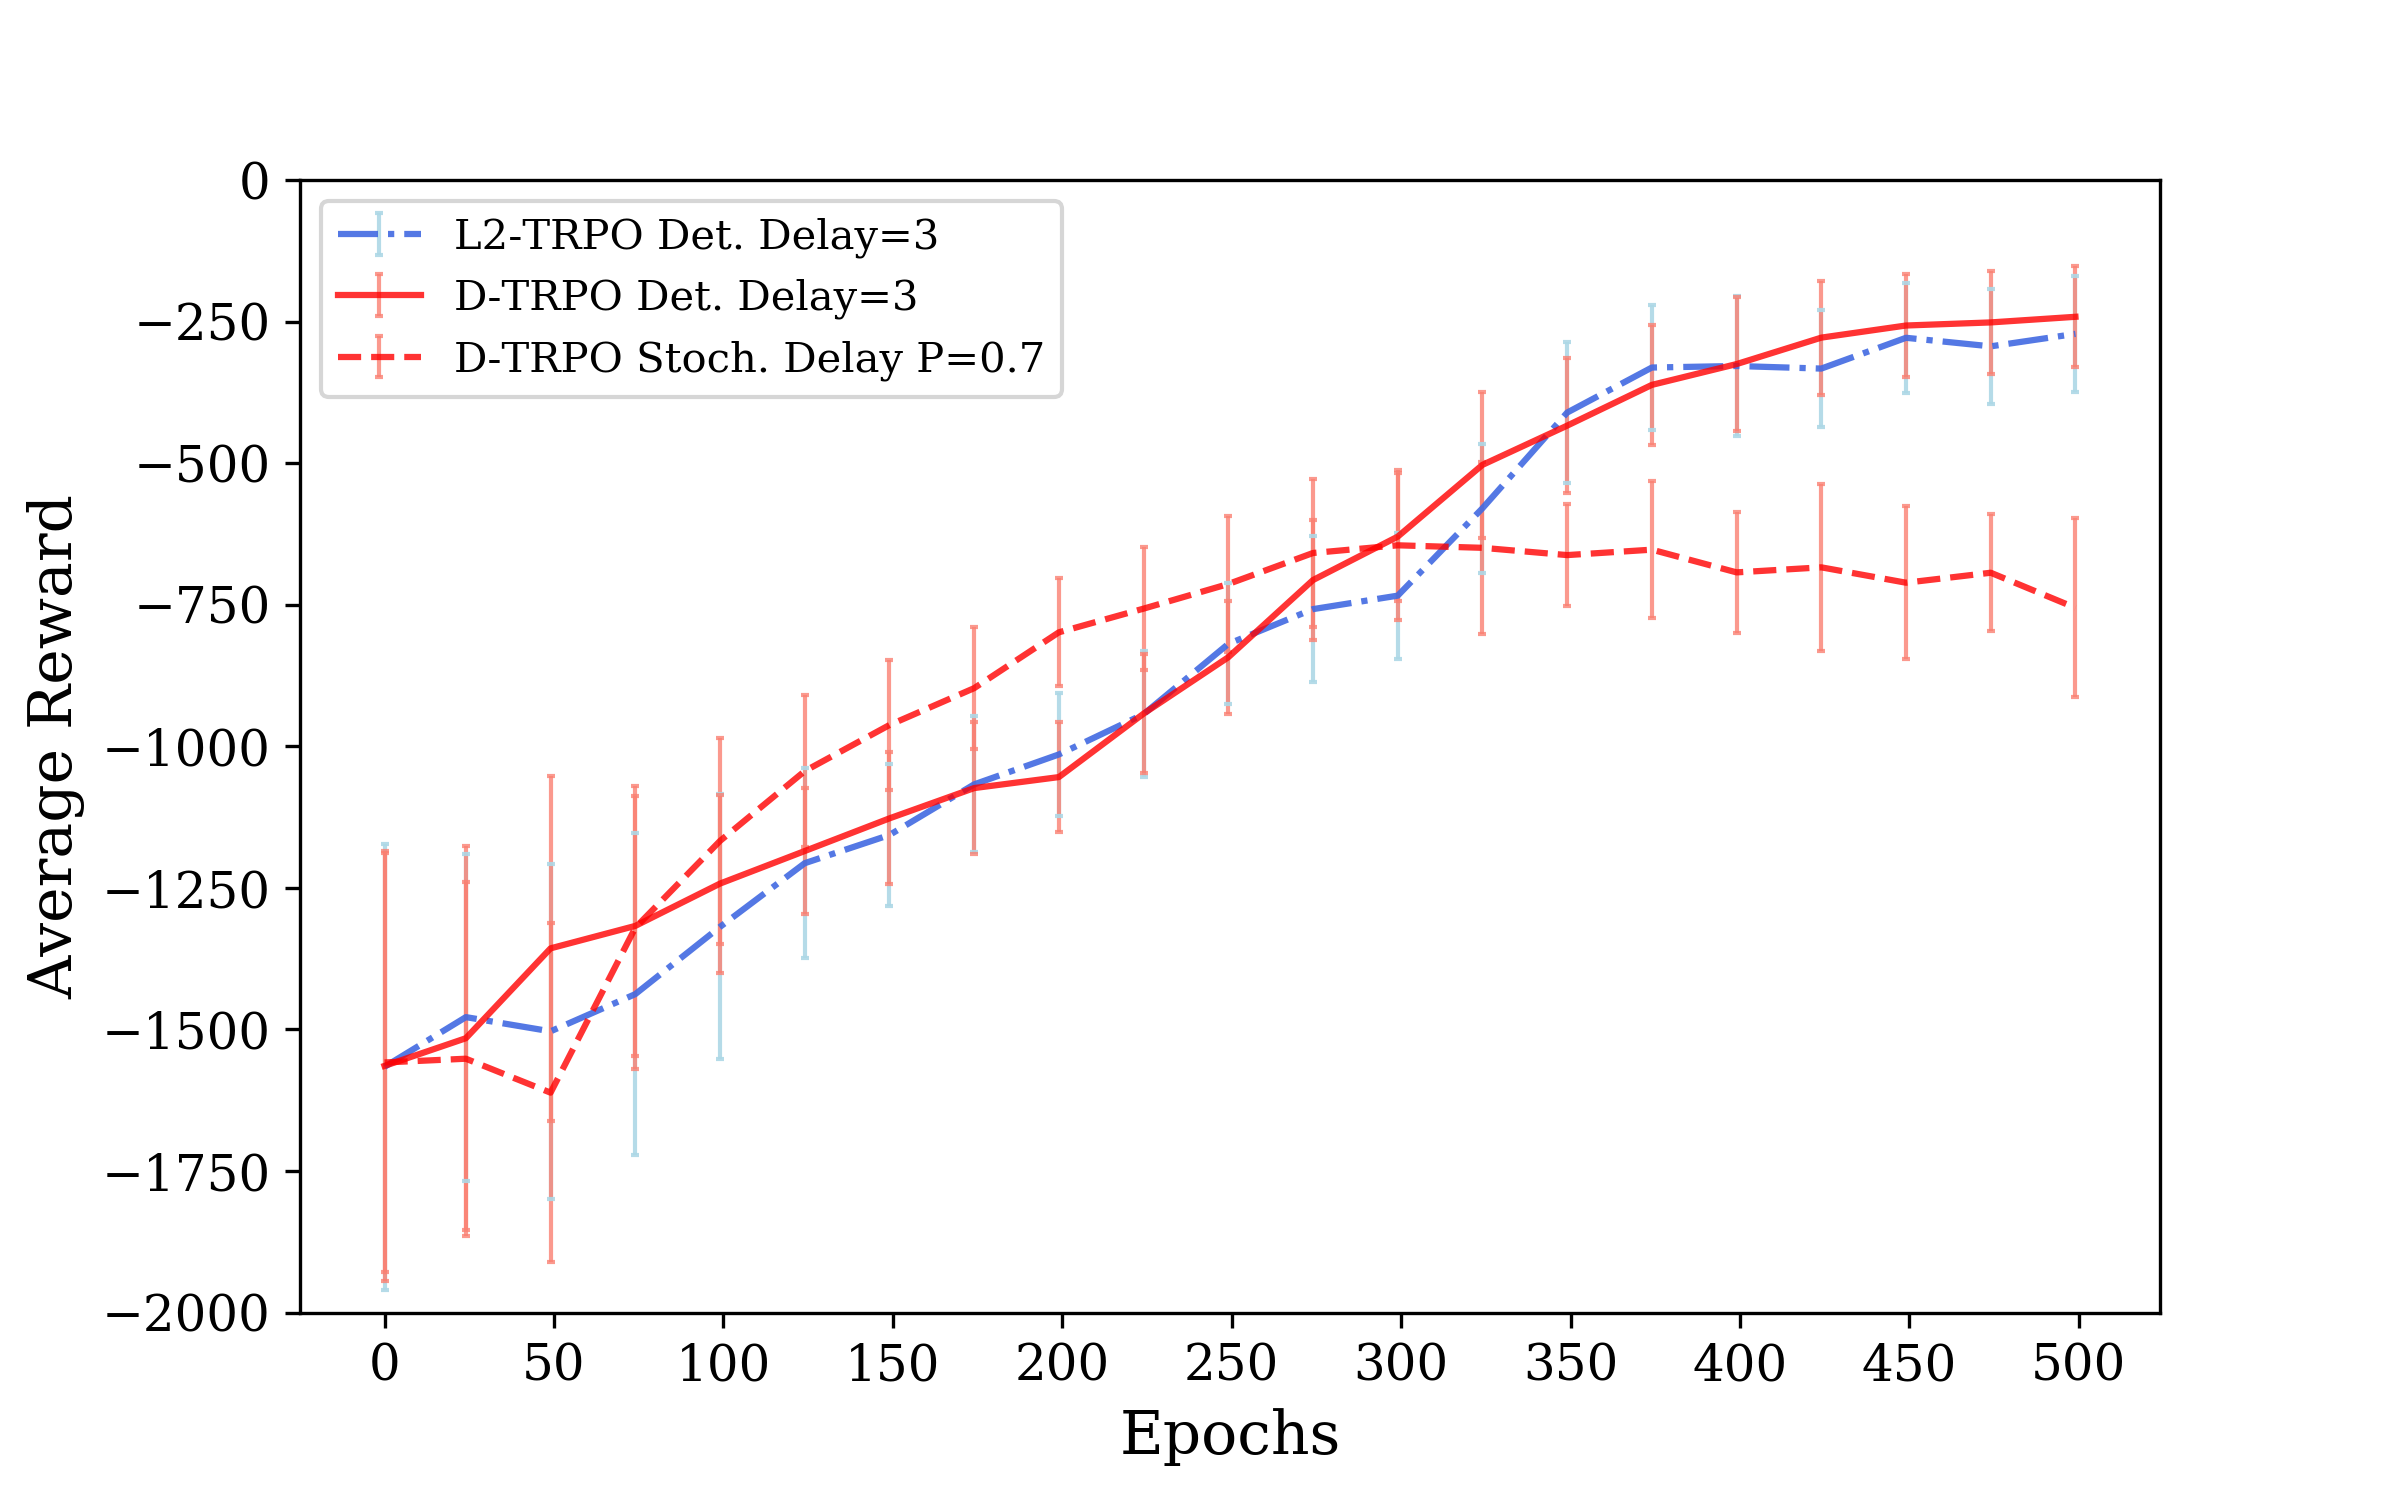
\includegraphics[width=15cm, keepaspectratio]{images/results/delayp07_comparisons_1.png}
                \caption{Training results obtained with a stochastic delay process $p=0.7$ and deterministic environment setting.}
                \label{fig:results_delayp07_1}
            \end{figure}
            
            \begin{figure}[hbtp]
                \centering
                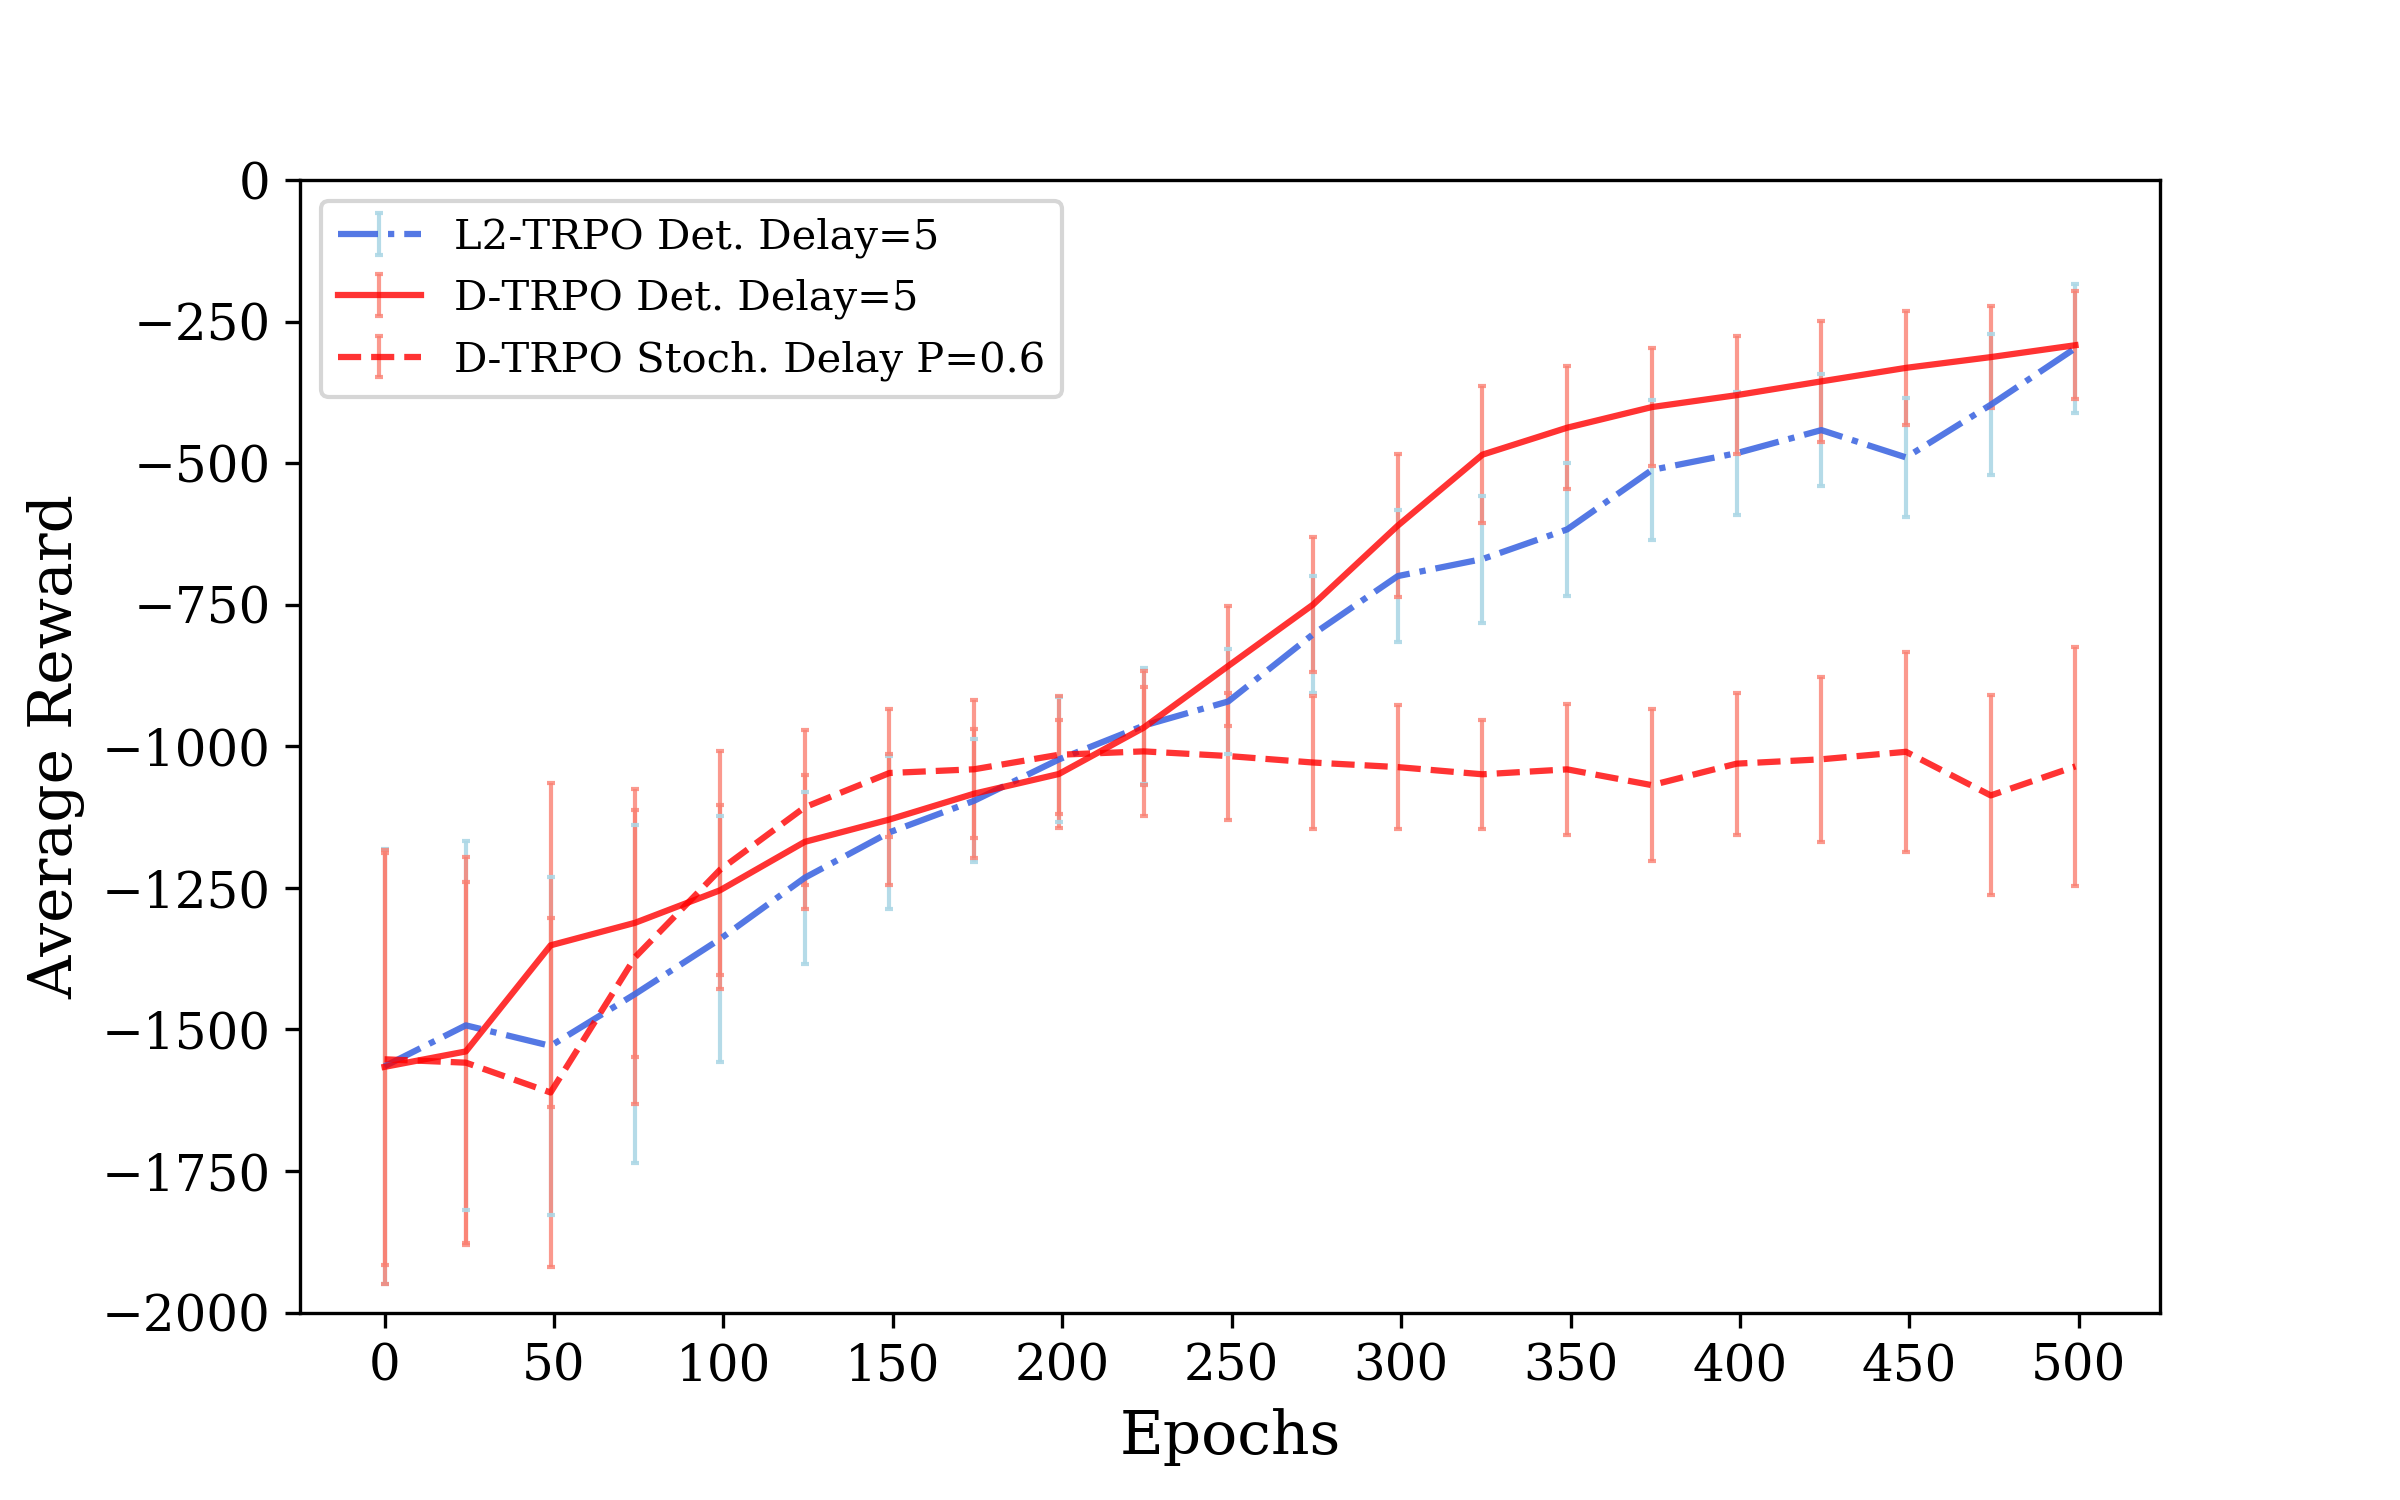
\includegraphics[width=15cm, keepaspectratio]{images/results/delayp06_comparisons_1.png}
                \caption{Training results obtained with a stochastic delay process $p=0.6$ and deterministic environment setting.}
                \label{fig:results_delayp06_1}
                
                \vspace{1.5cm}
                
                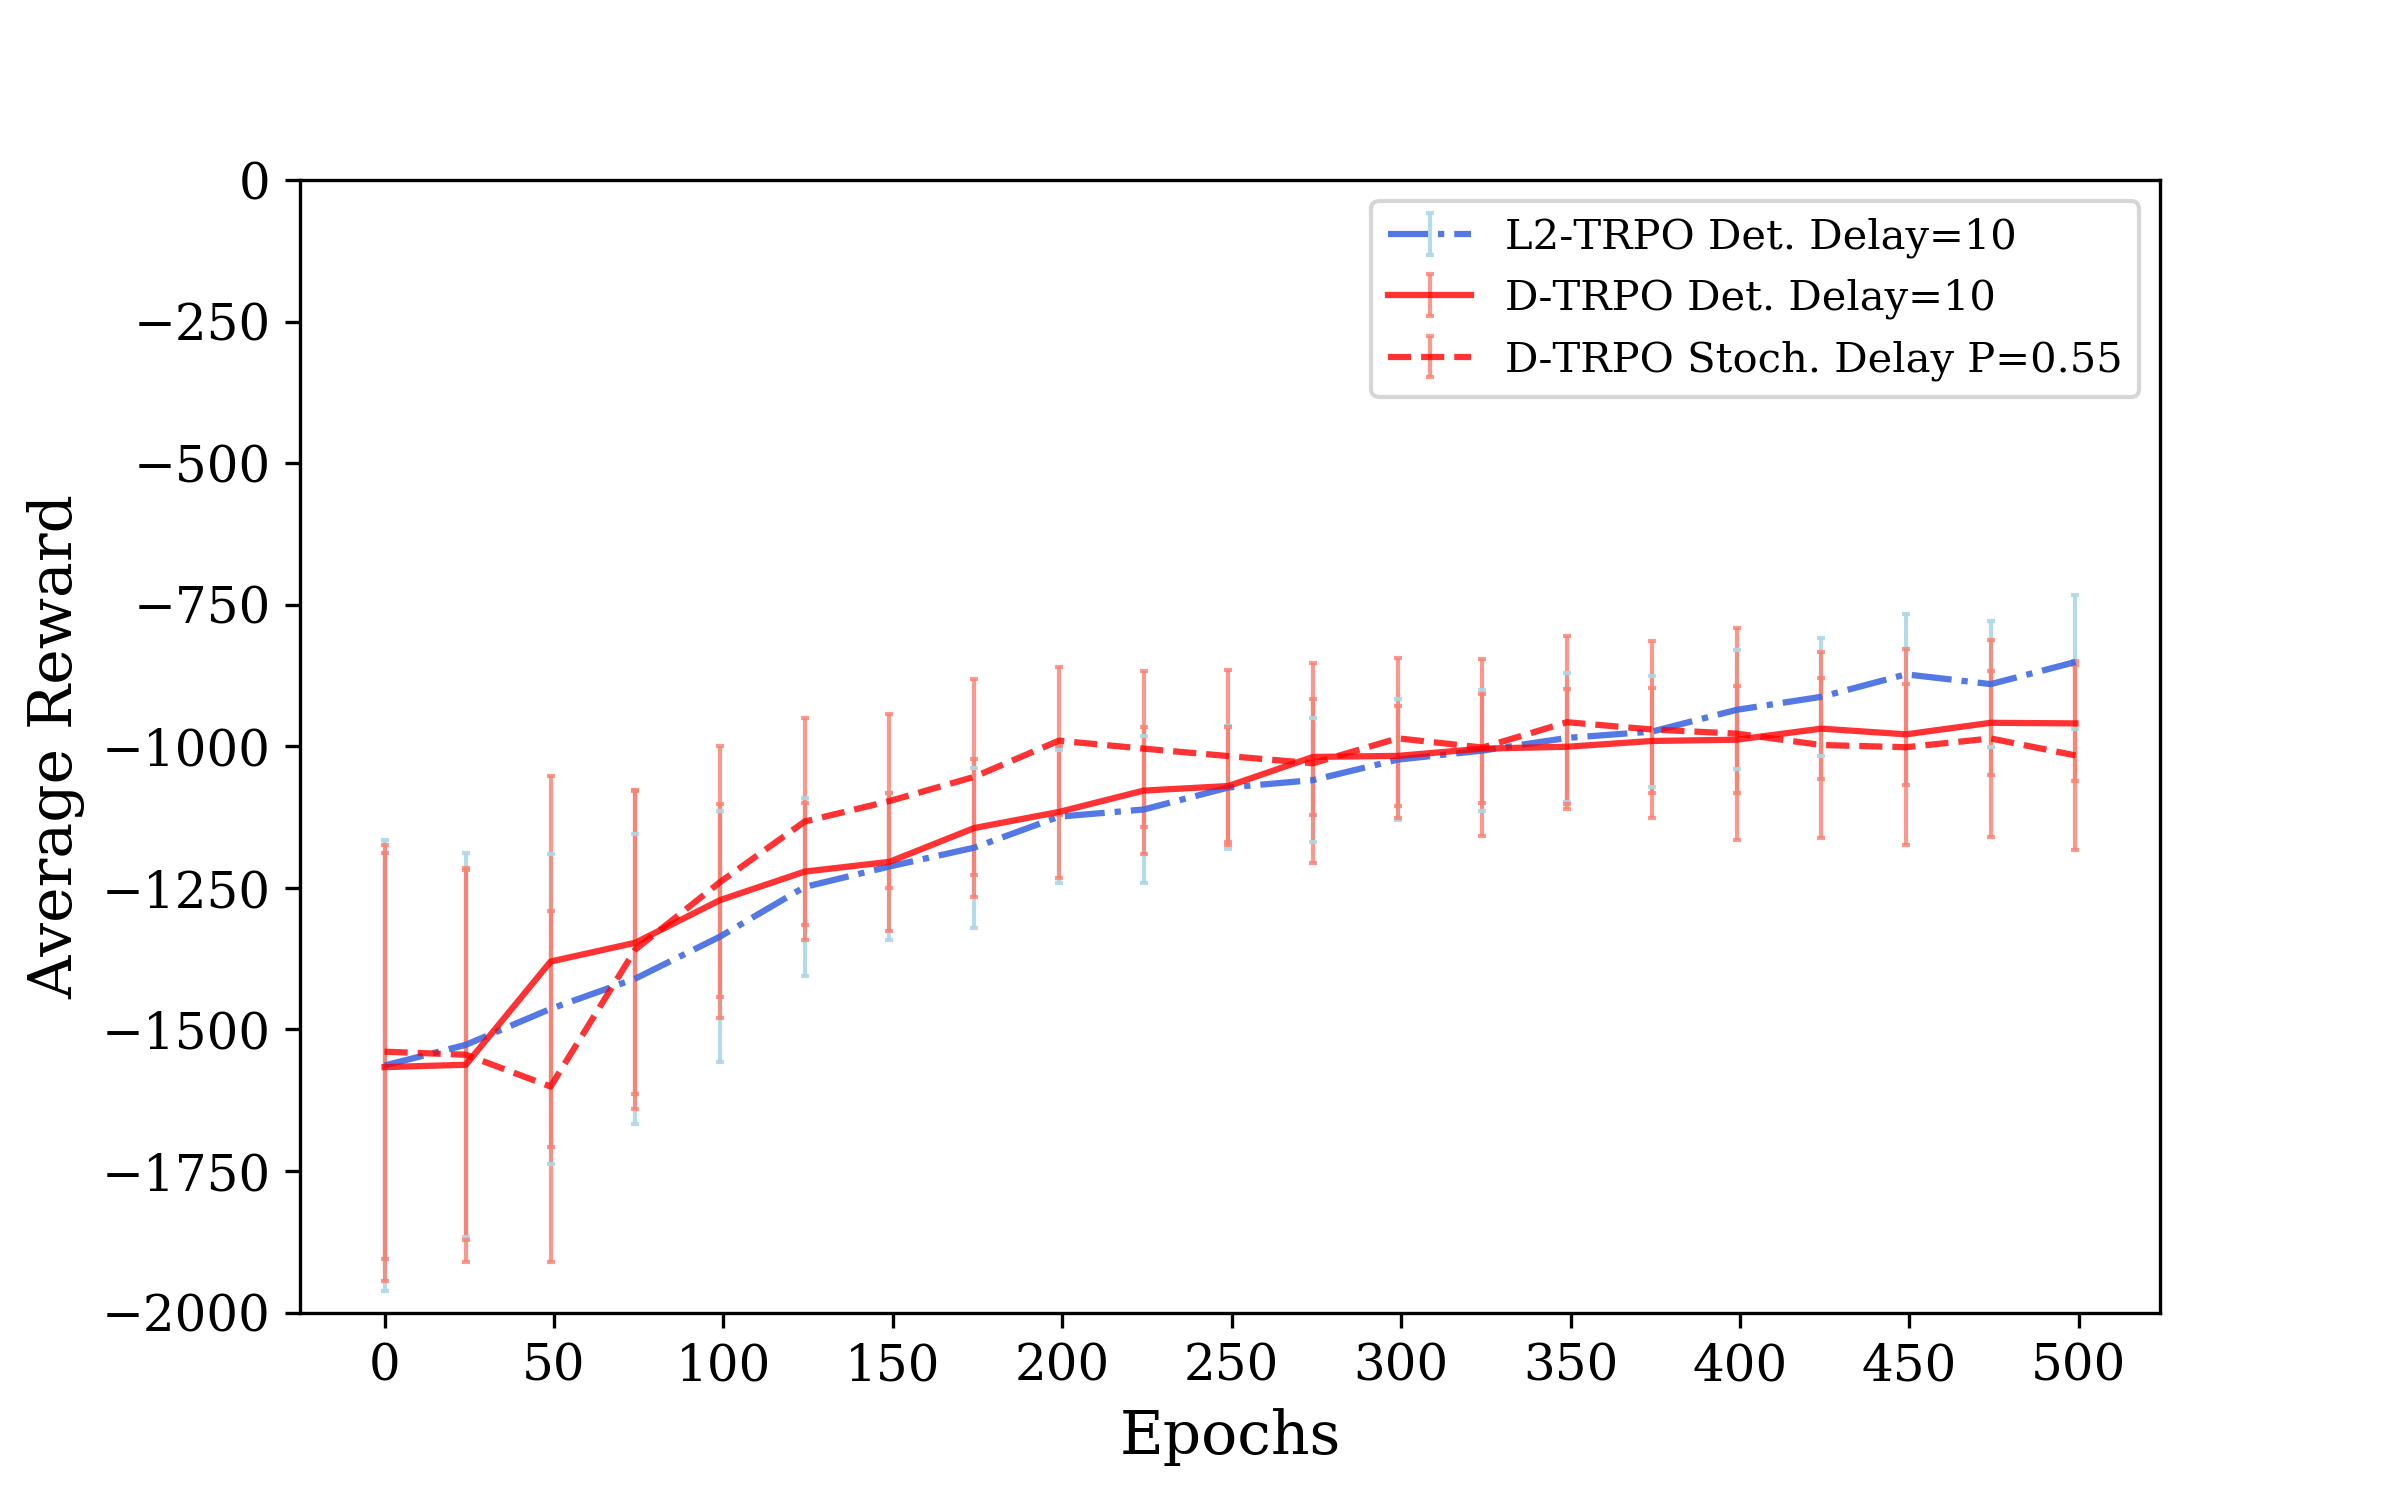
\includegraphics[width=15cm, keepaspectratio]{images/results/delayp05_comparisons_1.png}
                \caption{Training results obtained with a stochastic delay process $p=0.55$ and deterministic environment setting.}
                \label{fig:results_delayp05_1}
            \end{figure}
        
        \newpage
        \subsection{Test Results}
        \label{sub:res_test_delays}
            % Describe the behaviour of the trained models when tested on different delays w.r.t. the one they were trained with, both DTRPO and L2TRPO
            One of the strongest aspects of the proposed module is its compatibility with variable-sized input sequence, which does not only means it is possible to be trained natively with stochastic delays, but that it is also possible to test learnt model with different delay settings. In particular, we are interested in understanding how the models behave in the following two contexts:
            \begin{itemize}
                \setlength\itemsep{0.05em}
                \item The module has been trained with a certain amount of deterministic delay, but it is deployed in a setting with lower or higher deterministic delay. 
                \item The module has been trained with a certain amount of deterministic delay, but it is deployed in a stochastically delayed environment.
            \end{itemize}
            
            \subsubsection{Different Deterministic Delays Tests}
            
                \begin{table}[!b]
                    \makebox[\textwidth][c]{
                        \begin{tabular}{@{}ccccc@{}}
                        \toprule
                        \multicolumn{1}{c}{Test Setup} & 3-Steps Delay         & 5-Steps Delay        & 10-Steps Delay        & 15-Steps Delay        \\ \midrule
                        3-Steps Delay                  & -168.13 $\pm$ 102.28  & -793.21 $\pm$ 160.0  & -1210.73 $\pm$ 83.8   & -1554.17 $\pm$ 96.41  \\
                        5-Steps Delay                  & -171.12 $\pm$ 93.01   & -173.79 $\pm$ 92.2   & -1284.35 $\pm$ 85.96  & -1473.35 $\pm$ 110.78 \\
                        10-Steps Delay                 & -256.76 $\pm$ 110.75  & -246.86 $\pm$ 117.75 & -368.42 $\pm$ 126.98  & -1342.76 $\pm$ 170.88 \\
                        15-Steps Delay                 & -917.9 $\pm$ 87.04    & -902.22 $\pm$ 85.35  & -871.62 $\pm$ 102.85  & -956.13 $\pm$ 104.48  \\ \bottomrule
                        \end{tabular}
                    }
                    \centering
                    \caption{L2-TRPO trained on deterministic delays, denoted in the rows header, and Tested on deterministic delays, denoted in the columns header.}
                    \label{tab:l2trpo_det_det}
                \end{table}
                
                \begin{table}[!b]
                    \makebox[\textwidth][c]{
                        \begin{tabular}{@{}ccccc@{}}
                        \toprule
                        \multicolumn{1}{c}{Test Setup} & 3-Steps Delay         & 5-Steps Delay           & 10-Steps Delay          & 15-Steps Delay        \\ \midrule
                        3-Steps Delay                  & -155.61  $\pm$ 79.02  & -831.79 $\pm$ 127.55    & -1223.33 $\pm$ 71.02    & -1631.23 $\pm$ 77.32  \\
                        5-Steps Delay                  & -544.46  $\pm$ 105.17 & -175.36  $\pm$ 95.01    & -1161.79 $\pm$ 71.96    & -1578.53 $\pm$ 100.6  \\
                        10-Steps Delay                 & -1120.52 $\pm$ 56.54  & -1054.0  $\pm$ 65.79    & -720.49  $\pm$ 93.85    & -1352.81 $\pm$ 105.87 \\
                        15-Steps Delay                 & -1196.11 $\pm$ 66.82  & -1139.92 $\pm$ 83.66    & -1103.9  $\pm$ 76.88    & -912.31  $\pm$ 93.59  \\ \bottomrule
                        \end{tabular}
                    }
                    \centering
                    \caption{D-TRPO trained on deterministic delays, denoted in the rows header, and tested on deterministic delays, denoted in the columns header}
                    \label{tab:dtrpo_det_det}
                \end{table}
                
                Presented in Table \ref{tab:l2trpo_det_det}, L2-TRPO results are straightforward: each model trained with a certain amount of delay is also able to perform as well when tested on smaller delays, but it is not able to perform at all when tested on larger delays. This behaviour results from the definition of L2-TRPO loss function, which optimizes the module towards predictions of each unobserved state $s_{t-d+i}$, with $1 \leq i \leq d$, the Agent has traversed after the last observed state $s_{t-d}$, rather than only predicting the current unobserved state $s_t$. \newline
                D-TRPO shows a similar behaviour but its performances on smaller delays, albeit better than on larger delays, are significantly affected. Results are shown in Table \ref{tab:dtrpo_det_det}. The main reason behind this behavior lies in the interaction between the Belief-Estimation module and the policy/value networks. During training, the module takes as input extended states of the same size at each time-step and the output belief representation handled to policy/value networks reflects this property in its structure. Conceptually speaking, changing the size of the extended states has the same effect on the belief representation as changing language in a translation: for example, if D-TRPO is trained with 10 steps of delay, each of the 10 belief representations learnt by the module is built with its own "language". Policy and value networks learn the belief representations in the "10th-step language" only and they are able to improve the Agent's performances during training. However, this test is specifically targeting this assumption by letting the models interact against environments with a different delays, thus with extended states with different lengths. The results is that the module is outputting a belief representation that may be correct, but it's in a different "language" than policy and value networks expect and the Agent is not able to act accordingly. \newline
                At last, it is also possible to observe that, for both D-TRPO and L2-TRPO, in order to obtain the best possible performance we need to train the model with the same exact number of delay steps, thus confirming results from \pcite{delay:ssbm}, presented in Section \ref{subs:modelbasedapproach}.
                
            \subsubsection{Stochastic Delays Tests}
            
                \begin{table}[!b]
                    \centering
                    \begin{tabular}{@{}cccc@{}}
                    \toprule
                    \multicolumn{1}{c}{Test Setup} & Delay P=0.7           & Delay P=0.6          & Delay P=0.55         \\ \midrule
                    3-Steps Delay                  & -341.51 $\pm$ 131.67  & -609.37 $\pm$ 197.77 & -855.96 $\pm$ 238.89 \\
                    5-Steps Delay                  & -222.01 $\pm$ 118.2   & -430.42 $\pm$ 195.56 & -715.21 $\pm$ 262.44 \\
                    10-Steps Delay                 & -254.52 $\pm$ 147.07  & -306.1  $\pm$ 159.17 & -464.1  $\pm$ 235.38 \\
                    15-Steps Delay                 & -896.88 $\pm$ 78.9    & -903.66 $\pm$ 83.73  & -913.02 $\pm$ 109.81 \\ \bottomrule
                    \end{tabular}
                    \centering
                    \caption{L2-TRPO trained on deterministic delays, denoted in the rows header, and tested on stochastic delays, denoted in the columns header.}
                    \label{tab:l2trpo_det_stoch}
                \end{table}
                
                \begin{table}[!b]
                    \centering
                    \begin{tabular}{@{}cccc@{}}
                    \toprule
                    \multicolumn{1}{c}{Test Setup} & Delay P=0.7           & Delay P=0.6            & Delay P=0.55          \\ \midrule
                    3-Steps Delay                  & -344.15 $\pm$ 149.93  & -610.1 $\pm$ 196.71    & -883.26 $\pm$ 226.18  \\
                    5-Steps Delay                  & -605.38 $\pm$ 112.22  & -659.11 $\pm$ 147.38   & -800.12 $\pm$ 186.03  \\
                    10-Steps Delay                 & -1100.71 $\pm$ 68.2   & -1055.5 $\pm$ 83.53    & -1045.56 $\pm$ 104.81 \\
                    15-Steps Delay                 & -1196.4 $\pm$ 72.23   & -1158.42 $\pm$ 81.97   & -1131.19 $\pm$ 96.66  \\ \bottomrule
                    \end{tabular}
                    \centering
                    \caption{D-TRPO trained on deterministic delays, denoted in the rows header, and tested on stochastic delays, denoted in the columns header.}
                    \label{tab:dtrpo_det_stoch}
                \end{table}
                
                L2-TRPO confirms results obtained in the previous test in Table \ref{tab:l2trpo_det_stoch}. When a L2-TRPO model is tested with a stochastic delay process whose samples are generally less than or equal to the training constant delay, the module is able to build precise state predictions and the model is able to perform well, in some cases even close to the performances obtained when tested on deterministic delays. Lower performances across the tests are expected: the stochastic delay process is able to sample delays that are higher than the constant delay the model is trained with, thus the module is not able to provide a precise prediction at each time-step. \newline
                As expected, Table \ref{tab:dtrpo_det_stoch} shows that D-TRPO is suffering from the same issues discovered in the previous test. Performances are higher when the stochastic delay processes samples delays that are closer to the one the model has been trained with. While the 3-steps delay model is performing as well as the L2-TRPO counterpart, performances quickly decrease with both larger training delays and more difficult stochastic delay processes.
            
    \newpage
    \section{Stochastic Environment}
    \label{results:stochastic}
        % DTRPO vs L2TRPO
        This last Section is dedicated to experiments in a stochastic environment. It is divided into two sub-section: while Section \ref{sub:stoch_noise_impl} is concerned with explaining the stochastic environment implementation, Section \ref{sub:stoch_env_res} discusses the obtained results. We tested D-TRPO and L2-TRPO, both with the same hyperparameters explained in Section \ref{results:deterministic} in an environment affected by 5 steps of delay. Models are trained for 1000 epochs, each of them composed by 5000 steps for a total of 5 million steps. Single trajectories last for 250 steps. 
        
        \subsection{Stochastic Noise Implementation}
        \label{sub:stoch_noise_impl}
        % Explain each noise
            Stochastic environment implementation is reached by adding a stochastic perturbation to the sequence of actions chosen by the Agent while interacting in the Inverted Pendulum environment. In practice, at each time-step $t$, the Agent selects an action $a_t$, then a perturbation $\epsilon_t$ is sampled from a probability distribution and the action executed in the environment is $a_t + \epsilon_t$. We implemented perturbations sampled from the following probability distributions: Beta distribution with $\alpha=2$ and $\beta=2$, referred to as Quadratic; Beta distribution with $\alpha=0.5$ and $\beta=0.5$, referred to as U-Shaped; Beta distribution with $\alpha=8$ and $\beta=2$; LogNormal distribution with zero mean and both 0.1 and 1 standard deviation and a Triangular distribution in [-2, 2] with mode at 1. The shape of each distributions is shown in Figure \ref{fig:noises_all}.
        
            \begin{figure}
                \vspace{4.0cm}
                \centering
                \begin{subfigure}[b]{0.45\textwidth}
                    \centering
                    \includegraphics[width=\textwidth]{images/results/noises_beta_dist.png}
                    \caption{Shape of a Beta distribution with $\alpha=8$ and $\beta=2$.}
                    \label{fig:noises_beta_dist}
                \end{subfigure}
                \hfill
                \begin{subfigure}[b]{0.45\textwidth}
                    \centering
                    \includegraphics[width=\textwidth]{images/results/noises_quad_dist.png}
                    \caption{Shape of a Quadratic distribution (Beta with $\alpha=2$ and $\beta=2$).}
                    \label{fig:noises_quad_dist}
                \end{subfigure}
                \hfill
                \begin{subfigure}[b]{0.45\textwidth}
                    \centering
                    \includegraphics[width=\textwidth]{images/results/noises_ush_dist.png}
                    \caption{Shape of an U-Shaped distribution (Beta with $\alpha=0.5$ and $\beta=0.5$).}
                    \label{fig:noises_ush_dist}
                \end{subfigure}
                \hfill
                \begin{subfigure}[b]{0.45\textwidth}
                    \centering
                    \includegraphics[width=\textwidth]{images/results/noises_logns_dist.png}
                    \caption{Shape of a LogNormal distribution with STD=0.1.}
                    \label{fig:noises_logns_dist}
                \end{subfigure}
                \hfill
                \begin{subfigure}[b]{0.45\textwidth}
                    \centering
                    \includegraphics[width=\textwidth]{images/results/noises_logn_dist.png}
                    \caption{Shape of a LogNormal distribution with STD=1.0.}
                    \label{fig:noises_logn_dist}
                \end{subfigure}
                \hfill
                \begin{subfigure}[b]{0.45\textwidth}
                    \centering
                    \includegraphics[width=\textwidth]{images/results/noises_tri_dist.png}
                    \caption{Shape of a Triangular distribution, with mode at 1.}
                    \label{fig:noises_tri_dist}
                \end{subfigure}
                \caption{Shape of each Perturbation distribution. }
                \label{fig:noises_all}
            \end{figure}
            
        \subsection{Results}
        \label{sub:stoch_env_res}
        % Comment results
            From Figure \ref{fig:results_beta_1} to Figure \ref{fig:results_tri_1} training results are shown along with a comparison against D-TRPO and L2-TRPO trained with the same delay in the deterministic environment, in order to observe the impact of each stochastic perturbation. Across all the stochastic perturbations, it is possible to observe a great impact in the overall performance of both D-TRPO and L2-TRPO when compared to their deterministic environment counterpart. However, it is possible to identify two different behaviour across all tests:
            \begin{itemize}
                \setlength\itemsep{0.05em}
                \item Both D-TRPO and L2-TRPO heavily suffers from the presence of the stochastic perturbation, as in the case of LogNormal with STD=1.0, U-Shaped and Triangular perturbations, and their performances are aligned;
                \item Even if the decrease of performances is evident for both algorithms, D-TRPO shows a systematic improvement w.r.t. L2-TRPO, such in the cases of Beta(8,2), Quadratic and LogNormal with STD=0.1 perturbations.
            \end{itemize}
            The latter behaviour is promising, since it reveals that D-TRPO is able to significantly outperform L2-TRPO in several tests, which in turn means that the MAF network approach reveals to be beneficial w.r.t. the more standard approach of state prediction in the case of stochastic environments. 
            
            \begin{figure}[hbtp]
                \centering
                \includegraphics[width=11cm, keepaspectratio]{images/results/noises_beta_comparison_1.png}
                \caption{Training results obtained with deterministic delay of 5 steps and a Beta(8,2) perturbation.}
                \label{fig:results_beta_1}
                
                \includegraphics[width=11cm, keepaspectratio]{images/results/noises_quad_comparison_1.png}
                \caption{Training results obtained with deterministic delay of 5 steps and a Quadratic perturbation.}
                \label{fig:results_quad_1}
                
                \includegraphics[width=11cm, keepaspectratio]{images/results/noises_ush_comparison_1.png}
                \caption{Training results obtained with deterministic delay of 5 steps and a U-Shaped perturbation.}
                \label{fig:results_ush_1}
            \end{figure}
            
            \begin{figure}[hbtp]
                \centering
                \includegraphics[width=11cm, keepaspectratio]{images/results/noises_logns_comparison_1.png}
                \caption{Training results obtained with deterministic delay of 5 steps and a LogNormal perturbation with STD=0.1.}
                \label{fig:results_logns_1}
                
                \includegraphics[width=11cm, keepaspectratio]{images/results/noises_logn_comparison_1.png}
                \caption{Training results obtained with deterministic delay of 5 steps and a LogNormal perturbation with STD=1.0.}
                \label{fig:results_logn_1}
                
                \includegraphics[width=11cm, keepaspectratio]{images/results/noises_tri_comparison_1.png}
                \caption{Training results obtained with deterministic delay of 5 steps and a Triangular perturbation.}
                \label{fig:results_tri_1}
            \end{figure}
    \chapter{Conclusions and Future Research Directions}
    %   - Implement a solution that updates both Policy and Belief Module at the same time
    %       such as PSD and RPSP do. 
    %   - Test of different environments type to show strengths/weaknesses of the approach
    %   - Using the entire Transformer other than only the Encoder
    %   - Anonymous Delays applications
    
    %-------------------- BIBLIOGRAPHY ---------------------%
    \printbibliography[heading=bibintoc]
\end{document}
